% Options for packages loaded elsewhere
\PassOptionsToPackage{unicode}{hyperref}
\PassOptionsToPackage{hyphens}{url}
%
\documentclass[
]{article}
\usepackage{amsmath,amssymb}
\usepackage{lmodern}
\usepackage{iftex}
\ifPDFTeX
  \usepackage[T1]{fontenc}
  \usepackage[utf8]{inputenc}
  \usepackage{textcomp} % provide euro and other symbols
\else % if luatex or xetex
  \usepackage{unicode-math}
  \defaultfontfeatures{Scale=MatchLowercase}
  \defaultfontfeatures[\rmfamily]{Ligatures=TeX,Scale=1}
\fi
% Use upquote if available, for straight quotes in verbatim environments
\IfFileExists{upquote.sty}{\usepackage{upquote}}{}
\IfFileExists{microtype.sty}{% use microtype if available
  \usepackage[]{microtype}
  \UseMicrotypeSet[protrusion]{basicmath} % disable protrusion for tt fonts
}{}
\makeatletter
\@ifundefined{KOMAClassName}{% if non-KOMA class
  \IfFileExists{parskip.sty}{%
    \usepackage{parskip}
  }{% else
    \setlength{\parindent}{0pt}
    \setlength{\parskip}{6pt plus 2pt minus 1pt}}
}{% if KOMA class
  \KOMAoptions{parskip=half}}
\makeatother
\usepackage{xcolor}
\IfFileExists{xurl.sty}{\usepackage{xurl}}{} % add URL line breaks if available
\IfFileExists{bookmark.sty}{\usepackage{bookmark}}{\usepackage{hyperref}}
\hypersetup{
  hidelinks,
  pdfcreator={LaTeX via pandoc}}
\urlstyle{same} % disable monospaced font for URLs
\usepackage{color}
\usepackage{fancyvrb}
\newcommand{\VerbBar}{|}
\newcommand{\VERB}{\Verb[commandchars=\\\{\}]}
\DefineVerbatimEnvironment{Highlighting}{Verbatim}{commandchars=\\\{\}}
% Add ',fontsize=\small' for more characters per line
\newenvironment{Shaded}{}{}
\newcommand{\AlertTok}[1]{\textcolor[rgb]{1.00,0.00,0.00}{\textbf{#1}}}
\newcommand{\AnnotationTok}[1]{\textcolor[rgb]{0.38,0.63,0.69}{\textbf{\textit{#1}}}}
\newcommand{\AttributeTok}[1]{\textcolor[rgb]{0.49,0.56,0.16}{#1}}
\newcommand{\BaseNTok}[1]{\textcolor[rgb]{0.25,0.63,0.44}{#1}}
\newcommand{\BuiltInTok}[1]{\textcolor[rgb]{0.00,0.50,0.00}{#1}}
\newcommand{\CharTok}[1]{\textcolor[rgb]{0.25,0.44,0.63}{#1}}
\newcommand{\CommentTok}[1]{\textcolor[rgb]{0.38,0.63,0.69}{\textit{#1}}}
\newcommand{\CommentVarTok}[1]{\textcolor[rgb]{0.38,0.63,0.69}{\textbf{\textit{#1}}}}
\newcommand{\ConstantTok}[1]{\textcolor[rgb]{0.53,0.00,0.00}{#1}}
\newcommand{\ControlFlowTok}[1]{\textcolor[rgb]{0.00,0.44,0.13}{\textbf{#1}}}
\newcommand{\DataTypeTok}[1]{\textcolor[rgb]{0.56,0.13,0.00}{#1}}
\newcommand{\DecValTok}[1]{\textcolor[rgb]{0.25,0.63,0.44}{#1}}
\newcommand{\DocumentationTok}[1]{\textcolor[rgb]{0.73,0.13,0.13}{\textit{#1}}}
\newcommand{\ErrorTok}[1]{\textcolor[rgb]{1.00,0.00,0.00}{\textbf{#1}}}
\newcommand{\ExtensionTok}[1]{#1}
\newcommand{\FloatTok}[1]{\textcolor[rgb]{0.25,0.63,0.44}{#1}}
\newcommand{\FunctionTok}[1]{\textcolor[rgb]{0.02,0.16,0.49}{#1}}
\newcommand{\ImportTok}[1]{\textcolor[rgb]{0.00,0.50,0.00}{\textbf{#1}}}
\newcommand{\InformationTok}[1]{\textcolor[rgb]{0.38,0.63,0.69}{\textbf{\textit{#1}}}}
\newcommand{\KeywordTok}[1]{\textcolor[rgb]{0.00,0.44,0.13}{\textbf{#1}}}
\newcommand{\NormalTok}[1]{#1}
\newcommand{\OperatorTok}[1]{\textcolor[rgb]{0.40,0.40,0.40}{#1}}
\newcommand{\OtherTok}[1]{\textcolor[rgb]{0.00,0.44,0.13}{#1}}
\newcommand{\PreprocessorTok}[1]{\textcolor[rgb]{0.74,0.48,0.00}{#1}}
\newcommand{\RegionMarkerTok}[1]{#1}
\newcommand{\SpecialCharTok}[1]{\textcolor[rgb]{0.25,0.44,0.63}{#1}}
\newcommand{\SpecialStringTok}[1]{\textcolor[rgb]{0.73,0.40,0.53}{#1}}
\newcommand{\StringTok}[1]{\textcolor[rgb]{0.25,0.44,0.63}{#1}}
\newcommand{\VariableTok}[1]{\textcolor[rgb]{0.10,0.09,0.49}{#1}}
\newcommand{\VerbatimStringTok}[1]{\textcolor[rgb]{0.25,0.44,0.63}{#1}}
\newcommand{\WarningTok}[1]{\textcolor[rgb]{0.38,0.63,0.69}{\textbf{\textit{#1}}}}
\usepackage{longtable,booktabs,array}
\usepackage{calc} % for calculating minipage widths
% Correct order of tables after \paragraph or \subparagraph
\usepackage{etoolbox}
\makeatletter
\patchcmd\longtable{\par}{\if@noskipsec\mbox{}\fi\par}{}{}
\makeatother
% Allow footnotes in longtable head/foot
\IfFileExists{footnotehyper.sty}{\usepackage{footnotehyper}}{\usepackage{footnote}}
\makesavenoteenv{longtable}
\usepackage{graphicx}
\makeatletter
\def\maxwidth{\ifdim\Gin@nat@width>\linewidth\linewidth\else\Gin@nat@width\fi}
\def\maxheight{\ifdim\Gin@nat@height>\textheight\textheight\else\Gin@nat@height\fi}
\makeatother
% Scale images if necessary, so that they will not overflow the page
% margins by default, and it is still possible to overwrite the defaults
% using explicit options in \includegraphics[width, height, ...]{}
\setkeys{Gin}{width=\maxwidth,height=\maxheight,keepaspectratio}
% Set default figure placement to htbp
\makeatletter
\def\fps@figure{htbp}
\makeatother
\setlength{\emergencystretch}{3em} % prevent overfull lines
\providecommand{\tightlist}{%
  \setlength{\itemsep}{0pt}\setlength{\parskip}{0pt}}
\setcounter{secnumdepth}{-\maxdimen} % remove section numbering
\ifLuaTeX
  \usepackage{selnolig}  % disable illegal ligatures
\fi

\author{}
\date{}

\begin{document}

\begin{itemize}
\item
  \protect\hyperlink{1-unit-i-introduction-to-microprocessor}{1. Unit I:
  Introduction to Microprocessor}

  \begin{itemize}
  \item
    \protect\hyperlink{11-definition-and-history-of-microprocessors}{1.1.
    Definition and History of Microprocessors}
  \item
    \protect\hyperlink{12-basic-components-of-a-digital-computer}{1.2.
    Basic Components of a Digital Computer}
  \item
    \protect\hyperlink{13-basic-components-of-a-microprocessor}{1.3.
    Basic Components of a Microprocessor}
  \item
    \protect\hyperlink{14-architectures}{1.4. Architectures}

    \begin{itemize}
    \item
      \protect\hyperlink{141-von-neumann-architecture}{1.4.1. Von
      Neumann Architecture}
    \item
      \protect\hyperlink{142-harvard-architecture}{1.4.2. Harvard
      Architecture}
    \item
      \protect\hyperlink{143-von-neumann-vs-harvard-architecture}{1.4.3.
      Von Neumann vs Harvard Architecture}
    \end{itemize}
  \item
    \protect\hyperlink{15-instruction-formats--related-terms}{1.5.
    Instruction Formats \& Related Terms}

    \begin{itemize}
    \item
      \protect\hyperlink{151-instruction-format}{1.5.1. Instruction
      Format}

      \begin{itemize}
      \item
        \protect\hyperlink{1511-opcode-operation-code}{1.5.1.1. Opcode
        (Operation Code)}
      \item
        \protect\hyperlink{1512-operand}{1.5.1.2. Operand}
      \item
        \protect\hyperlink{1513-example}{1.5.1.3. Example}
      \end{itemize}
    \item
      \protect\hyperlink{152-instruction-cycle}{1.5.2. Instruction
      Cycle}
    \item
      \protect\hyperlink{153-machine-cycle}{1.5.3. Machine Cycle}
    \item
      \protect\hyperlink{154-t-state-clock-cycle}{1.5.4. T-State (Clock
      Cycle)}
    \end{itemize}
  \item
    \protect\hyperlink{16-risc-vs-cisc}{1.6. RISC vs. CISC}
  \end{itemize}
\item
  \protect\hyperlink{2-unit-ii-working-of-8085-microprocessor}{2. Unit
  II: Working of 8085 Microprocessor}

  \begin{itemize}
  \item
    \protect\hyperlink{21-pin-diagram-of-8085}{2.1. Pin Diagram of 8085}

    \begin{itemize}
    \item
      \protect\hyperlink{211-power-supply-clock--reset-pins}{2.1.1.
      Power Supply, Clock \& Reset Pins}
    \item
      \protect\hyperlink{212-control-and-status-signal-pins}{2.1.2.
      Control and Status Signal Pins}

      \begin{itemize}
      \item
        \protect\hyperlink{2121-role-of-ale-signal-in-demultiplexing}{2.1.2.1.
        Role of ALE signal in Demultiplexing}
      \end{itemize}
    \item
      \protect\hyperlink{213-interrupt-pins}{2.1.3. Interrupt Pins}
    \item
      \protect\hyperlink{214-serial-communication-pins}{2.1.4. Serial
      Communication Pins}
    \item
      \protect\hyperlink{215-dma-pins}{2.1.5. DMA Pins}
    \end{itemize}
  \item
    \protect\hyperlink{22-block-diagram-of-8085}{2.2. Block Diagram of
    8085}

    \begin{itemize}
    \item
      \protect\hyperlink{221-arithmetic--logic-unit-alu-and-timing--control-unit-cu}{2.2.1.
      Arithmetic \& Logic Unit (ALU) and Timing \& Control Unit (CU)}
    \item
      \protect\hyperlink{222-registers}{2.2.2. Registers}
    \item
      \protect\hyperlink{223-instruction-register-instruction-decoder-and-machine-cycle-encoder}{2.2.3.
      Instruction Register, Instruction Decoder, and Machine Cycle
      Encoder}
    \item
      \protect\hyperlink{224-the-flag-register}{2.2.4. The Flag
      Register}
    \item
      \protect\hyperlink{225-bus-organization}{2.2.5. Bus Organization}
    \end{itemize}
  \item
    \protect\hyperlink{23-working-of-the-8085}{2.3. Working of the 8085}

    \begin{itemize}
    \item
      \protect\hyperlink{231-memory-interfacing}{2.3.1. Memory
      Interfacing}
    \item
      \protect\hyperlink{232-demultiplexing-of-lower-order-address-bus--data-bus}{2.3.2.
      Demultiplexing of Lower Order Address Bus \& Data Bus}
    \item
      \protect\hyperlink{233-instruction-fetching-decoding-and-execution}{2.3.3.
      Instruction Fetching, Decoding and Execution}

      \begin{itemize}
      \item
        \protect\hyperlink{2331-instruction-fetching}{2.3.3.1.
        Instruction Fetching}
      \item
        \protect\hyperlink{2332-instruction-decoding}{2.3.3.2.
        Instruction Decoding}
      \item
        \protect\hyperlink{2333-instruction-execution}{2.3.3.3.
        Instruction Execution}
      \item
        \protect\hyperlink{2334-example-add-b-instruction}{2.3.3.4.
        Example: ADD B Instruction}
      \end{itemize}
    \end{itemize}
  \item
    \protect\hyperlink{24-microprocessor-vs-microcontroller}{2.4.
    Microprocessor vs. Microcontroller}
  \end{itemize}
\item
  \protect\hyperlink{3-unit-iii-microcontroller-architecture}{3. Unit
  III: Microcontroller Architecture}

  \begin{itemize}
  \item
    \protect\hyperlink{31-general-block-diagram-of-a-microcontroller}{3.1.
    General Block Diagram of a Microcontroller}
  \item
    \protect\hyperlink{32-pin-diagram-of-8051}{3.2. Pin Diagram of 8051}
  \item
    \protect\hyperlink{33-8051-microcontroller-block-diagram}{3.3. 8051
    Microcontroller Block Diagram}

    \begin{itemize}
    \item
      \protect\hyperlink{331-alu-arithmetic-logic-unit--timing-and-control-unit}{3.3.1.
      ALU (Arithmetic Logic Unit) \& Timing and Control Unit}
    \item
      \protect\hyperlink{332-instruction-register-and-instruction-decoder}{3.3.2.
      Instruction Register and Instruction Decoder}
    \item
      \protect\hyperlink{333-accumulator-a}{3.3.3. Accumulator (A)}
    \item
      \protect\hyperlink{334-register-b}{3.3.4. Register B}
    \item
      \protect\hyperlink{335-pc-program-counter}{3.3.5. PC (Program
      Counter)}
    \item
      \protect\hyperlink{336-sp-stack-pointer}{3.3.6. SP (Stack
      Pointer)}
    \item
      \protect\hyperlink{337-dptr-data-pointer}{3.3.7. DPTR (Data
      Pointer)}
    \item
      \protect\hyperlink{338-special-function-registers-sfrs}{3.3.8.
      Special Function Registers (SFRs)}
    \item
      \protect\hyperlink{339-psw-program-status-word-address-0d0h-bit-addressable}{3.3.9.
      PSW: Program Status Word (Address: 0D0H, Bit addressable)}
    \item
      \protect\hyperlink{3310-clock--reset-circuit}{3.3.10. Clock \&
      Reset Circuit}
    \item
      \protect\hyperlink{3311-io-ports}{3.3.11. I/O Ports}

      \begin{itemize}
      \item
        \protect\hyperlink{33111-port-0-pin-structure}{3.3.11.1. Port-0
        Pin Structure}
      \item
        \protect\hyperlink{33112-port-1-pin-structure}{3.3.11.2. Port 1
        Pin Structure}
      \item
        \protect\hyperlink{33113-port-2-pin-structure}{3.3.11.3. Port 2
        Pin Structure}
      \item
        \protect\hyperlink{33114-port-3-pin-structure}{3.3.11.4. Port 3
        Pin Structure}
      \end{itemize}
    \end{itemize}
  \item
    \protect\hyperlink{34-memory-organization}{3.4. Memory Organization}

    \begin{itemize}
    \item
      \protect\hyperlink{341-program-memory-rom}{3.4.1. Program Memory
      (ROM)}
    \item
      \protect\hyperlink{342-data-memory-ram}{3.4.2. Data Memory (RAM)}
    \item
      \protect\hyperlink{343-external-memory-interfacing-and-decoding-logic}{3.4.3.
      External Memory Interfacing and Decoding Logic}
    \end{itemize}
  \item
    \protect\hyperlink{35-stack-stack-pointer-and-stack-operations}{3.5.
    Stack, Stack Pointer, and Stack Operations}
  \item
    \protect\hyperlink{36-timerscounters}{3.6. Timers/Counters}

    \begin{itemize}
    \item
      \protect\hyperlink{361-tcon-register}{3.6.1. TCON Register}
    \item
      \protect\hyperlink{362-tmod-register}{3.6.2. TMOD Register}
    \item
      \protect\hyperlink{363-modes-of-operation}{3.6.3. Modes of
      Operation}

      \begin{itemize}
      \item
        \protect\hyperlink{3631-timer-mode-0-13-bit-timer-mode}{3.6.3.1.
        Timer Mode 0 (13-bit Timer Mode)}
      \item
        \protect\hyperlink{3632-timer-mode-1-16-bit-timer-mode}{3.6.3.2.
        Timer Mode 1 (16-bit Timer Mode)}
      \item
        \protect\hyperlink{3633-timer-mode-2-8-bit-auto-reload-timer-mode}{3.6.3.3.
        Timer Mode 2 (8-bit Auto-Reload Timer Mode)}
      \item
        \protect\hyperlink{3634-timer-mode-3-split-timer-mode}{3.6.3.4.
        Timer Mode 3 (Split Timer Mode)}
      \end{itemize}
    \end{itemize}
  \item
    \protect\hyperlink{37-serial-communication}{3.7. Serial
    Communication}

    \begin{itemize}
    \item
      \protect\hyperlink{371-scon-register}{3.7.1. SCON Register}
    \item
      \protect\hyperlink{372-modes}{3.7.2. Modes}

      \begin{itemize}
      \item
        \protect\hyperlink{3721-mode-0-serial-communication-synchronous-shift-register-mode}{3.7.2.1.
        Mode 0 Serial Communication (Synchronous Shift Register Mode)}
      \item
        \protect\hyperlink{3722-mode-1-serial-communication-10-bit-uart-mode}{3.7.2.2.
        Mode 1 Serial Communication (10-bit UART Mode)}
      \item
        \protect\hyperlink{3723-mode-2-serial-communication-11-bit-uart-mode}{3.7.2.3.
        Mode 2 Serial Communication (11-bit UART Mode)}
      \item
        \protect\hyperlink{3724-mode-3-serial-communication-9-bit-uart-mode}{3.7.2.4.
        Mode 3 Serial Communication (9-bit UART Mode)}
      \end{itemize}
    \item
      \protect\hyperlink{373-pcon-register}{3.7.3. PCON Register}
    \end{itemize}
  \item
    \protect\hyperlink{38-interrupts}{3.8. Interrupts}

    \begin{itemize}
    \item
      \protect\hyperlink{381-ie-register}{3.8.1. IE Register}
    \item
      \protect\hyperlink{382-ip-register}{3.8.2. IP Register}
    \end{itemize}
  \end{itemize}
\item
  \protect\hyperlink{4-unit-iv-8051-programming}{4. Unit IV: 8051
  Programming}

  \begin{itemize}
  \item
    \protect\hyperlink{41-addressing-modes}{4.1. Addressing Modes}

    \begin{itemize}
    \item
      \protect\hyperlink{411-immediate-addressing-mode}{4.1.1. Immediate
      addressing mode}
    \item
      \protect\hyperlink{412-register-addressing-mode}{4.1.2. Register
      addressing mode}
    \item
      \protect\hyperlink{413-direct-addressing-mode}{4.1.3. Direct
      addressing mode}
    \item
      \protect\hyperlink{414-indirect-addressing-mode}{4.1.4. Indirect
      addressing mode}
    \item
      \protect\hyperlink{415-indexed-addressing-mode}{4.1.5. Indexed
      addressing mode}
    \item
      \protect\hyperlink{416-relative-addressing-mode}{4.1.6. Relative
      addressing mode}
    \item
      \protect\hyperlink{417-bit-addressing-mode}{4.1.7. Bit addressing
      mode}
    \end{itemize}
  \item
    \protect\hyperlink{42-8051-instruction-set}{4.2. 8051 Instruction
    Set}

    \begin{itemize}
    \item
      \protect\hyperlink{421-data-transfer-instructions}{4.2.1. Data
      Transfer Instructions}
    \item
      \protect\hyperlink{422-arithmetic-instructions}{4.2.2. Arithmetic
      Instructions}
    \item
      \protect\hyperlink{423-logical-instructions}{4.2.3. Logical
      Instructions}
    \item
      \protect\hyperlink{424-program-branching-instructions}{4.2.4.
      Program Branching Instructions}
    \item
      \protect\hyperlink{425-boolean-or-bit-manipulation-instructions}{4.2.5.
      Boolean or Bit-manipulation Instructions}
    \item
      \protect\hyperlink{426-machine-control}{4.2.6. Machine Control}
    \end{itemize}
  \item
    \protect\hyperlink{43-assembly-language-programming-examples}{4.3.
    Assembly Language Programming Examples}

    \begin{itemize}
    \item
      \protect\hyperlink{431-refer-dedicated-notes-for-programming-examples}{4.3.1.
      Refer Dedicated Notes for Programming Examples}
    \end{itemize}
  \end{itemize}
\item
  \protect\hyperlink{5-unit-v-interfacing--applications-of-microcontroller}{5.
  Unit V: Interfacing \& Applications of Microcontroller}

  \begin{itemize}
  \item
    \protect\hyperlink{51-interfacing-input-devices-or-sensors}{5.1.
    Interfacing Input Devices or Sensors}

    \begin{itemize}
    \item
      \protect\hyperlink{511-push-button-switches}{5.1.1. Push Button
      Switches}
    \item
      \protect\hyperlink{512-dip-switch}{5.1.2. DIP Switch}
    \item
      \protect\hyperlink{513-keypad-interfacing}{5.1.3. Keypad
      Interfacing}
    \item
      \protect\hyperlink{514-potentiometer-interfacing}{5.1.4.
      Potentiometer Interfacing}
    \item
      \protect\hyperlink{515-lm35-temperature-sensor}{5.1.5. LM35
      Temperature Sensor}
    \end{itemize}
  \item
    \protect\hyperlink{52-interfacing-output-devices-or-actuators}{5.2.
    Interfacing Output Devices or Actuators}

    \begin{itemize}
    \item
      \protect\hyperlink{521-leds}{5.2.1. LEDs}

      \begin{itemize}
      \item
        \protect\hyperlink{5211-blink-8-leds}{5.2.1.1. Blink 8 LEDs}
      \item
        \protect\hyperlink{5212-led-fading-using-pwm}{5.2.1.2. LED
        Fading using PWM}
      \end{itemize}
    \item
      \protect\hyperlink{522-7-segment-displays}{5.2.2. 7-Segment
      Displays}
    \item
      \protect\hyperlink{523-lcd-interfacing}{5.2.3. LCD Interfacing}
    \item
      \protect\hyperlink{524-relays}{5.2.4. Relays}
    \item
      \protect\hyperlink{525-dc-motors}{5.2.5. DC Motors}

      \begin{itemize}
      \item
        \protect\hyperlink{5251-l293d-ic}{5.2.5.1. L293D IC}
      \item
        \protect\hyperlink{5252-dc-motor-interfacing-with-8051}{5.2.5.2.
        DC Motor Interfacing with 8051}
      \end{itemize}
    \item
      \protect\hyperlink{526-stepper-motors}{5.2.6. Stepper Motors}

      \begin{itemize}
      \item
        \protect\hyperlink{5261-basics-of-stepper-motors}{5.2.6.1.
        Basics of Stepper Motors}
      \item
        \protect\hyperlink{5262-stepper-motor-interfacing-with-8051}{5.2.6.2.
        Stepper Motor Interfacing with 8051}
      \end{itemize}
    \end{itemize}
  \item
    \protect\hyperlink{53-adc-analog-to-digital-converter}{5.3. ADC
    (Analog-to-Digital Converter)}

    \begin{itemize}
    \item
      \protect\hyperlink{531-adc0804-interfacing}{5.3.1. ADC0804
      Interfacing}
    \end{itemize}
  \item
    \protect\hyperlink{54-dac-digital-to-analog-converter}{5.4. DAC
    (Digital-to-Analog Converter)}

    \begin{itemize}
    \item
      \protect\hyperlink{541-dac0808-interfacing}{5.4.1. DAC0808
      Interfacing}
    \item
      \protect\hyperlink{542-generate-ramp-signal-using-dac}{5.4.2.
      Generate Ramp Signal using DAC}
    \item
      \protect\hyperlink{543-generate-triangular-wave-using-dac}{5.4.3.
      Generate Triangular wave using DAC}
    \end{itemize}
  \item
    \protect\hyperlink{55-real-world-applications}{5.5. Real-World
    Applications}

    \begin{itemize}
    \item
      \protect\hyperlink{551-temperature-control-system-using-an-lm35-sensor}{5.5.1.
      Temperature control system using an LM35 sensor}
    \item
      \protect\hyperlink{552-gsm-based-security-system}{5.5.2. GSM based
      Security System}
    \item
      \protect\hyperlink{553-rpm-meter}{5.5.3. RPM meter}
    \end{itemize}
  \end{itemize}
\end{itemize}

\hypertarget{1-unit-i-introduction-to-microprocessor}{%
\section{1. Unit I: Introduction to
Microprocessor}\label{1-unit-i-introduction-to-microprocessor}}

\hypertarget{11-definition-and-history-of-microprocessors}{%
\subsection{1.1. Definition and History of
Microprocessors}\label{11-definition-and-history-of-microprocessors}}

\textbf{Definition of a Microprocessor}

A microprocessor is a single integrated circuit (IC) that incorporates
the core functions of a computer's central processing unit (CPU).

\begin{itemize}
\item
  \textbf{The "Brain" of a Computer:} It executes instructions, performs
  calculations, and manages the flow of data within a computer system.
\item
  \textbf{Small and Powerful:} Microprocessors pack millions or even
  billions of transistors into a tiny chip, enabling complex processing
  in compact devices.
\item
  \textbf{Essential for Modern Devices:} They power a vast range of
  devices from smartphones and laptops to cars, appliances, and
  industrial equipment.
\item
  \textbf{Components:} Typical components of a microprocessor include:

  \begin{itemize}
  \item
    Arithmetic Logic Unit (ALU) - Performs arithmetic and logical
    operations
  \item
    Control Unit (CU) - Decodes instructions and coordinates the
    operations of other units
  \item
    Registers - Small, high-speed memory locations for temporary data
    storage
  \end{itemize}
\item
  \textbf{Responsible for:}

  \begin{itemize}
  \item
    \textbf{Fetching instructions:} Retrieving instructions from the
    computer's memory.
  \item
    \textbf{Decoding instructions:} Translating instructions into a form
    the microprocessor understands.
  \item
    \textbf{Executing instructions:} Performing calculations and logical
    operations based on the instructions.
  \item
    \textbf{Controlling data flow:} Managing the movement of data
    between memory, input devices, output devices, and the
    microprocessor itself.
  \end{itemize}
\end{itemize}

\textbf{History}

The evolution of microprocessors is a fascinating story of technological
advancement:

\begin{itemize}
\item
  \textbf{Early Computers (1940s-1950s):} The first computers were
  massive, filling entire rooms. They used vacuum tubes for processing,
  which were bulky, power-hungry, and prone to failure.
\item
  \textbf{Transistors (1950s-1960s):} The invention of the transistor
  revolutionized electronics. Transistors were smaller, faster, and more
  reliable than vacuum tubes, leading to smaller and more powerful
  computers.
\item
  \textbf{Integrated Circuits (1960s):} Integrated circuits (ICs)
  combined multiple transistors, resistors, and other components onto a
  single chip. This enabled further miniaturization of computers.
\item
  \textbf{The First Microprocessor (1971):} Intel released the Intel
  4004, the first commercially available microprocessor on a single
  chip. While limited in power by today's standards, it paved the way
  for the computing revolution.
\item
  \textbf{Rapid Advancement (1970s-1980s):} This period saw exponential
  growth in microprocessor performance with the introduction of iconic
  processors like the Intel 8080, Zilog Z80, and Motorola 6800. These
  processors found their way into the first personal computers.
\item
  \textbf{Modern Era (1990s-Present):} Microprocessors have become
  incredibly powerful, with billions of transistors on a single chip.
  They power not only our computers but also smartphones, tablets, smart
  devices, cars, and countless other technologies.
\end{itemize}

\textbf{Key milestones in microprocessor history:}

\begin{itemize}
\item
  \textbf{1971:} Intel 4004 (4-bit)
\item
  \textbf{1974:} Intel 8080 (8-bit)
\item
  \textbf{1978:} Intel 8086 (16-bit) - foundation of the x86
  architecture used in many PCs today.
\item
  \textbf{1993:} Intel Pentium (32-bit) -- brought significant
  performance gains
\item
  \textbf{2000s:} Introduction of multi-core processors
\item
  \textbf{Present:} Continued focus on performance, power efficiency,
  and specialized microprocessors for tasks like AI and machine
  learning.
\end{itemize}

\hypertarget{12-basic-components-of-a-digital-computer}{%
\subsection{1.2. Basic Components of a Digital
Computer}\label{12-basic-components-of-a-digital-computer}}

\begin{figure}
\centering
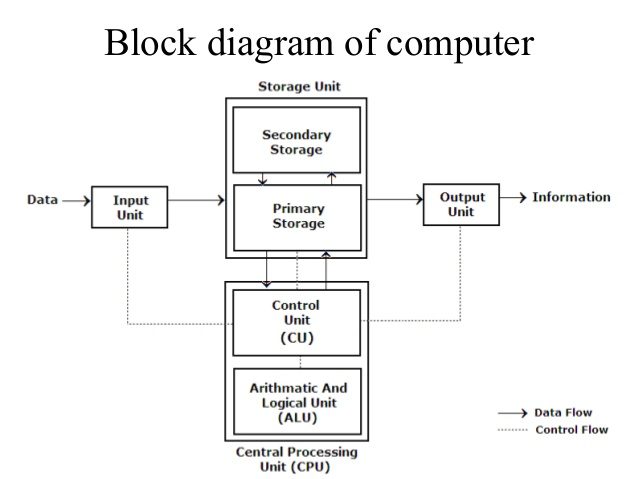
\includegraphics{/home/milav/Codes/MPMC/assets/imgs/181001_MCU_Question_Bank_Solved_html_871c3be60335b53b.jpg}
\caption{}
\end{figure}

A digital computer is a versatile device capable of performing
calculations and logical operations at incredible speeds. To achieve
this, a computer relies on several fundamental components working
together:

\begin{itemize}
\item
  \textbf{Input Unit:} This unit bridges the gap between the user and
  the computer. It allows data and instructions to be entered into the
  system. Some common input devices include:

  \begin{itemize}
  \item
    Keyboard
  \item
    Mouse
  \item
    Touchscreen
  \item
    Scanner
  \item
    Microphone
  \end{itemize}
\item
  \textbf{Storage Unit:} The storage unit preserves data, instructions,
  and results for short-term and long-term use. It's divided into two
  main categories:

  \begin{itemize}
  \item
    \textbf{Primary Storage (Main Memory):} This fast, but relatively
    expensive memory temporarily holds the currently running programs,
    input data, and intermediate calculations. Since primary storage is
    volatile, data is lost when the computer powers down. RAM (Random
    Access Memory) is the most common type of primary storage.
  \item
    \textbf{Secondary Storage (Auxiliary Memory):}

    This type of storage acts as a permanent repository for programs,
    data, and the operating system. It's slower than primary storage but
    offers larger capacity at a lower cost. Examples include:

    \begin{itemize}
    \item
      Hard Disk Drives (HDD)
    \item
      Solid-State Drives (SSD)
    \item
      Optical Disks (CDs, DVDs)
    \end{itemize}
  \end{itemize}
\item
  \textbf{Central Processing Unit (CPU):} The CPU is the "brain" of the
  computer responsible for controlling and executing instructions. It
  contains two primary parts:

  \begin{itemize}
  \item
    \textbf{Control Unit (CU):} The orchestrator of the CPU. It fetches
    instructions from memory, decodes them, and generates signals to
    coordinate the activities of the other components within the system.
  \item
    \textbf{Arithmetic Logic Unit (ALU):} The heart of calculations. The
    ALU performs arithmetic operations (addition, subtraction, etc.) and
    logical operations (AND, OR, NOT, etc.).
  \end{itemize}
\item
  \textbf{Output Unit:} The output unit presents the results of
  processing to the user in a human-readable form. Examples include:

  \begin{itemize}
  \item
    Monitor (display)
  \item
    Printer
  \item
    Speakers
  \end{itemize}
\end{itemize}

\textbf{How These Components Work Together}

\begin{enumerate}
\def\labelenumi{\arabic{enumi}.}
\item
  \textbf{Input:} A user enters data or instructions through an input
  device like a keyboard or mouse.
\item
  \textbf{Storage:} Data and instructions are temporarily stored in the
  main memory (RAM) for quick access by the CPU.
\item
  \textbf{Processing:}

  \begin{itemize}
  \item
    The Control Unit fetches an instruction from memory and decodes it.
  \item
    The ALU executes the instruction, potentially involving calculations
    or logical comparisons.
  \item
    Results might be stored back into memory (RAM or secondary storage).
  \end{itemize}
\item
  \textbf{Output:} The processed results are presented to the user
  through an output device, such as a monitor or printer.
\end{enumerate}

\hypertarget{13-basic-components-of-a-microprocessor}{%
\subsection{1.3. Basic Components of a
Microprocessor}\label{13-basic-components-of-a-microprocessor}}

\textbf{CPU (Central Processing Unit)}

\begin{itemize}
\item
  \textbf{The Brain:} The CPU is the heart of a microprocessor,
  responsible for interpreting and executing instructions. Think of it
  as the decision-maker and coordinator of the entire system.
\item
  Key Components:

  \begin{itemize}
  \item
    \textbf{Control Unit (CU):} The manager that fetches instructions
    from memory, decodes them, and controls the flow of data and
    operations throughout the processor.
  \item
    \textbf{Arithmetic Logic Unit (ALU):} The "calculator" within the
    CPU that performs all arithmetic (addition, subtraction, etc.) and
    logical (AND, OR, NOT, etc.) operations.
  \end{itemize}
\end{itemize}

\textbf{ALU (Arithmetic and Logic Unit)}

\begin{itemize}
\item
  \textbf{The Calculator:} The ALU is a core part of the CPU, dedicated
  to carrying out the calculations and logic comparisons that drive
  computations within the microprocessor.
\item
  Operations:

  \begin{itemize}
  \item
    Arithmetic: Addition, subtraction, multiplication, division, etc.
  \item
    Logical: AND, OR, XOR, NOT, comparisons, etc.
  \end{itemize}
\end{itemize}

\textbf{Control Unit}

\begin{itemize}
\item
  \textbf{The Orchestrator:} The control unit is another essential part
  of the CPU. It directs all operations within the microprocessor.
\item
  Responsibilities:

  \begin{itemize}
  \item
    \textbf{Instruction Fetching:} Retrieves instructions from memory.
  \item
    \textbf{Instruction Decoding:} Interprets instructions to determine
    what needs to be done.
  \item
    \textbf{Control Signals:} Generates signals to coordinate the ALU,
    memory, and other components, ensuring everything works in sync.
  \end{itemize}
\end{itemize}

\textbf{Memory Unit (RAM, ROM)}

\begin{itemize}
\item
  \textbf{Data and Code Storage:} The memory unit is where the
  microprocessor stores important data and instructions.
\item
  Types:

  \begin{itemize}
  \item
    \textbf{RAM (Random Access Memory):} Temporary, fast storage used
    for currently running programs and data. It's volatile, meaning data
    disappears when the power goes off.
  \item
    \textbf{ROM (Read-Only Memory):} Permanent storage that typically
    holds the computer's startup instructions (BIOS) and other essential
    data that shouldn't change.
  \end{itemize}
\end{itemize}

\textbf{Input/Output (I/O) Units}

\begin{itemize}
\item
  \textbf{Communication Bridge:} These units facilitate communication
  between the microprocessor and the outside world.
\item
  Input Devices:

  \begin{itemize}
  \item
    Keyboard
  \item
    Mouse
  \item
    Scanner
  \item
    Microphone
  \item
    Network interface card
  \end{itemize}
\item
  Output Devices:

  \begin{itemize}
  \item
    Monitor
  \item
    Printer
  \item
    Speakers
  \item
    Network interface card
  \end{itemize}
\end{itemize}

\textbf{How It All Works Together}

\begin{enumerate}
\def\labelenumi{\arabic{enumi}.}
\item
  \textbf{Fetch:} The Control Unit fetches an instruction from memory
  (RAM).
\item
  \textbf{Decode:} The Control Unit decodes the instruction to figure
  out the required operation.
\item
  \textbf{Execute:}

  \begin{itemize}
  \item
    If it's a calculation or logical operation, the ALU gets involved.
  \item
    Data may be moved between memory, the ALU, and internal registers
    (tiny, super-fast memory within the CPU).
  \end{itemize}
\item
  \textbf{Store:} Results might be written back to memory or sent to an
  output device.
\end{enumerate}

\hypertarget{14-architectures}{%
\subsection{1.4. Architectures}\label{14-architectures}}

\hypertarget{141-von-neumann-architecture}{%
\subsubsection{1.4.1. Von Neumann
Architecture}\label{141-von-neumann-architecture}}

\begin{itemize}
\item
  \textbf{Key Features:}

  \begin{itemize}
  \item
    \textbf{Single Unified Memory:} Both instructions and data reside in
    the same memory space.
  \item
    \textbf{Single Bus:} A shared bus is used for transferring both data
    and instructions.
  \item
    \textbf{Sequential Execution:} Instructions are fetched and executed
    one at a time.
  \end{itemize}
\item
  \textbf{Components:}

  \begin{itemize}
  \item
    Central Processing Unit (CPU) with Control Unit (CU) \& Arithmetic
    Logic Unit (ALU)
  \item
    Unified Memory
  \item
    Input/Output (I/O) devices
  \item
    Bus
  \end{itemize}
\item
  \textbf{Advantages:}

  \begin{itemize}
  \item
    \textbf{Simplicity:} Easier to design and implement.
  \item
    \textbf{Flexibility:} Programs can modify their own code, enabling
    dynamic behavior.
  \end{itemize}
\item
  \textbf{Limitations:}

  \begin{itemize}
  \item
    \textbf{The von Neumann Bottleneck:} Limited bandwidth due to the
    shared data and instruction bus, potentially slowing down
    processing.
  \item
    \textbf{Security Concerns:} Less separation between code and data
    can increase vulnerability to some types of cyber-attacks.
  \end{itemize}
\end{itemize}

\hypertarget{142-harvard-architecture}{%
\subsubsection{1.4.2. Harvard
Architecture}\label{142-harvard-architecture}}

\begin{itemize}
\item
  \textbf{Key Features:}

  \begin{itemize}
  \item
    \textbf{Separate Memories:} Distinct memory units for instructions
    and data.
  \item
    \textbf{Dedicated Buses:} Separate buses for fetching instructions
    and accessing data.
  \item
    \textbf{Parallel Execution:} The CPU can access instructions and
    data simultaneously.
  \end{itemize}
\item
  \textbf{Components:}

  \begin{itemize}
  \item
    Central Processing Unit (CPU) with Control Unit (CU) \& Arithmetic
    Logic Unit (ALU)
  \item
    Separate instruction and data memory
  \item
    Dedicated buses for each memory
  \item
    Input/Output (I/O) devices
  \end{itemize}
\item
  \textbf{Advantages:}

  \begin{itemize}
  \item
    \textbf{Speed and Efficiency:} Parallel access offers faster
    execution and eliminates the bottleneck present in Von Neumann
    architectures.
  \item
    \textbf{Enhanced Security:} Improved isolation between code and data
    can aid security measures.
  \item
    \textbf{Deterministic Behavior:} Reliable timing and performance
    make it ideal for real-time systems.
  \end{itemize}
\item
  \textbf{Limitations:}

  \begin{itemize}
  \item
    \textbf{Increased Complexity:} More complex to design due to
    additional memory units and buses.
  \item
    \textbf{Less Flexible for Self-Modifying Code:} Separating code and
    data makes it more difficult for programs to modify their
    instructions on the fly.
  \end{itemize}
\end{itemize}

\hypertarget{143-von-neumann-vs-harvard-architecture}{%
\subsubsection{1.4.3. Von Neumann vs Harvard
Architecture}\label{143-von-neumann-vs-harvard-architecture}}

\textbf{Similarities}

\begin{itemize}
\item
  \textbf{Fundamental Components:} Both architectures include a CPU
  (with CU and ALU), memory, and I/O devices.
\item
  \textbf{Stored-Program Concept:} Both can store programs in memory and
  execute them.
\end{itemize}

\textbf{Differences Summary Table}

\begin{longtable}[]{@{}lll@{}}
\toprule
Feature & Von Neumann Architecture & Harvard Architecture \\
\midrule
\endhead
Memory Structure & Single unified memory for instructions and data &
Separate memory spaces for instructions and data \\
Buses & Single bus for instructions and data & Separate, dedicated buses
for instructions and data \\
Instruction Processing & Sequential & Potential for parallel instruction
fetch and data access \\
Performance & Potential bottleneck due to shared bus & Faster,
eliminates the bottleneck \\
Complexity & Simpler to design and implement & Increased hardware
complexity \\
Flexibility & Programs can self-modify code & Less flexible for
self-modifying code \\
Security & Less isolation between code and data & Improved isolation \\
Applications & General-purpose computers, laptops, servers. & Embedded
systems, microcontrollers, digital signal processors (DSPs). \\
Diagram &
\href{http://www.polytechnichub.com/wp-content/uploads/2017/04/Harvard-architecture.jpg}{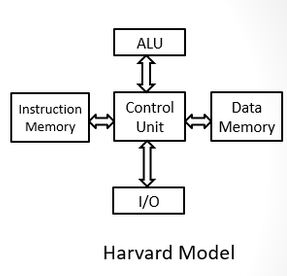
\includegraphics{/home/milav/Codes/MPMC/assets/imgs/181001_MCU_Question_Bank_Solved_html_aa3957193cea79df.jpg}}
&
\href{http://www.polytechnichub.com/wp-content/uploads/2017/04/Von-Neumann-architecture.jpg}{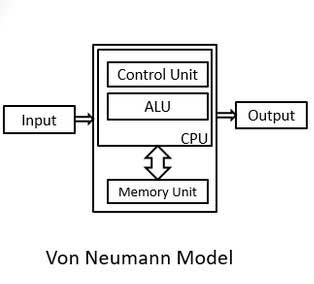
\includegraphics{/home/milav/Codes/MPMC/assets/imgs/181001_MCU_Question_Bank_Solved_html_29b2dc6bc518dc80.jpg}} \\
\bottomrule
\end{longtable}

\hypertarget{15-instruction-formats--related-terms}{%
\subsection{1.5. Instruction Formats \& Related
Terms}\label{15-instruction-formats--related-terms}}

\hypertarget{151-instruction-format}{%
\subsubsection{1.5.1. Instruction Format}\label{151-instruction-format}}

A microprocessor instruction is a fundamental command encoded in binary
that tells the microprocessor to perform a specific operation.
Instructions generally have two core parts:

\hypertarget{1511-opcode-operation-code}{%
\paragraph{1.5.1.1. Opcode (Operation
Code)}\label{1511-opcode-operation-code}}

Specifies the operation the microprocessor should perform (e.g., add,
subtract, move data, compare). The opcode is a unique binary pattern
assigned to a particular action.

\hypertarget{1512-operand}{%
\paragraph{1.5.1.2. Operand}\label{1512-operand}}

Data the operation acts upon. An operand could be:

\begin{itemize}
\item
  \textbf{Immediate Value:} Data directly included in the instruction
  itself.
\item
  \textbf{Register:} A small, fast memory location inside the processor.
\item
  \textbf{Memory Address:} A location in the main memory.
\end{itemize}

\hypertarget{1513-example}{%
\paragraph{1.5.1.3. Example}\label{1513-example}}

Consider a simple 'ADD' instruction in a hypothetical microprocessor:

\begin{Shaded}
\begin{Highlighting}[]
\NormalTok{ADD  R1,  \#5}
\end{Highlighting}
\end{Shaded}

\begin{itemize}
\item
  \textbf{Opcode:} 'ADD' tells the processor to perform an addition
  operation.
\item
  \textbf{Operands}:

  \begin{itemize}
  \item
    'R1' is a register, indicating one value for the addition is stored
    in register R1.
  \item
    '\#5' is an immediate value, specifying the second value for the
    addition.
  \end{itemize}
\end{itemize}

\hypertarget{152-instruction-cycle}{%
\subsubsection{1.5.2. Instruction Cycle}\label{152-instruction-cycle}}

The instruction cycle is the complete sequence of steps a microprocessor
takes to process a single instruction. It involves:

\begin{enumerate}
\def\labelenumi{\arabic{enumi}.}
\item
  \textbf{Fetch:} The Control Unit retrieves the instruction's opcode
  from memory.
\item
  \textbf{Decode:} The Control Unit decodes the opcode to understand the
  required operation.
\item
  \textbf{Execute}:

  The instruction is carried out. This may involve:

  \begin{itemize}
  \item
    Reading data from memory or registers.
  \item
    Performing calculations or logical operations in the ALU.
  \item
    Writing results back to memory or registers.
  \end{itemize}
\end{enumerate}

\hypertarget{153-machine-cycle}{%
\subsubsection{1.5.3. Machine Cycle}\label{153-machine-cycle}}

A machine cycle represents a single, indivisible action performed by the
microprocessor necessary to carry out part of an instruction's
operation. Some examples of machine cycles include:

\begin{itemize}
\item
  \textbf{Memory Read:} Fetching data from memory.
\item
  \textbf{Memory Write:} Storing data into memory.
\item
  \textbf{I/O Read:} Reading data from an input device.
\item
  \textbf{I/O Write:} Sending data to an output device.
\end{itemize}

An instruction cycle often comprises multiple machine cycles.

\hypertarget{154-t-state-clock-cycle}{%
\subsubsection{1.5.4. T-State (Clock
Cycle)}\label{154-t-state-clock-cycle}}

A T-state is the fundamental unit of time in a microprocessor, measured
by a single period of the processor's internal clock. Each machine cycle
typically takes one or more T-states. Faster clocks mean more T-states
per second, facilitating faster processing.

\textbf{Relationship}

\begin{itemize}
\item
  \textbf{Instructions} are built from opcodes and operands.
\item
  An \textbf{instruction cycle} consists of the steps to execute one
  complete instruction.
\item
  A \textbf{machine cycle} is a smaller unit of action within an
  instruction cycle.
\item
  \textbf{T-States} are the fundamental timing unit, with a machine
  cycle usually encompassing multiple T-states.
\end{itemize}

Instructions in the 8085 microprocessor can be 1, 2, or 3 bytes long.
The structure varies depending on the specific instruction and the
addressing modes used.

\hypertarget{16-risc-vs-cisc}{%
\subsection{1.6. RISC vs. CISC}\label{16-risc-vs-cisc}}

\begin{longtable}[]{@{}lll@{}}
\toprule
Feature & RISC (Reduced Instruction Set Computer) & CISC (Complex
Instruction Set Computer) \\
\midrule
\endhead
Instruction Set & Smaller, simpler instructions. Focus on individual
operations. & Larger, more complex instructions capable of multiple
operations within a single command. \\
Addressing Modes & Limited addressing modes. & Extensive addressing
modes for flexible data access. \\
Execution & Emphasizes hardware optimization. Instructions often execute
in one clock cycle. & Utilizes microcode to implement complex
instructions, potentially requiring multiple clock cycles per
instruction. \\
Compiler Design & Relies on simpler instructions, shifting complexity to
the compiler. & Simplifies compiler design by offloading complexity to
processor hardware. \\
Memory Access & Load/Store architecture: Data must be explicitly moved
between registers and memory for operations. & Instructions can operate
directly on memory. \\
Pipelining & Highly efficient pipelining. & Pipelining can be less
efficient due to variable-length instructions. \\
Register Usage & Large number of general-purpose registers for fast
operand access. & Fewer registers, often with specialized purposes. \\
Speed & Simplicity enables faster instruction execution, higher overall
throughput. & Compact code due to complex instructions can optimize
memory usage. \\
Power Efficiency & Efficient due to simpler design and execution. &
Reduced instruction count can lower power consumption in some cases. \\
Design Cost & Fewer transistors and simpler design can reduce
development time and cost. & More transistors and complex design can
increase development time and cost. \\
Code Size & Simpler instructions may require longer sequences to achieve
the same task, increasing program size. & Complex instructions can
increase complexity and potential for errors, impacting performance. \\
Compiler & Burden placed on the compiler to generate efficient code. &
Can hide hardware complexity, simplifying software development. \\
Applications & High-performance computing, smartphones, embedded
systems, devices where speed and power efficiency are crucial. & Legacy
systems, applications prioritizing code density (smaller program
size). \\
\bottomrule
\end{longtable}

\hypertarget{2-unit-ii-working-of-8085-microprocessor}{%
\section{2. Unit II: Working of 8085
Microprocessor}\label{2-unit-ii-working-of-8085-microprocessor}}

\hypertarget{21-pin-diagram-of-8085}{%
\subsection{2.1. Pin Diagram of 8085}\label{21-pin-diagram-of-8085}}

\begin{figure}
\centering
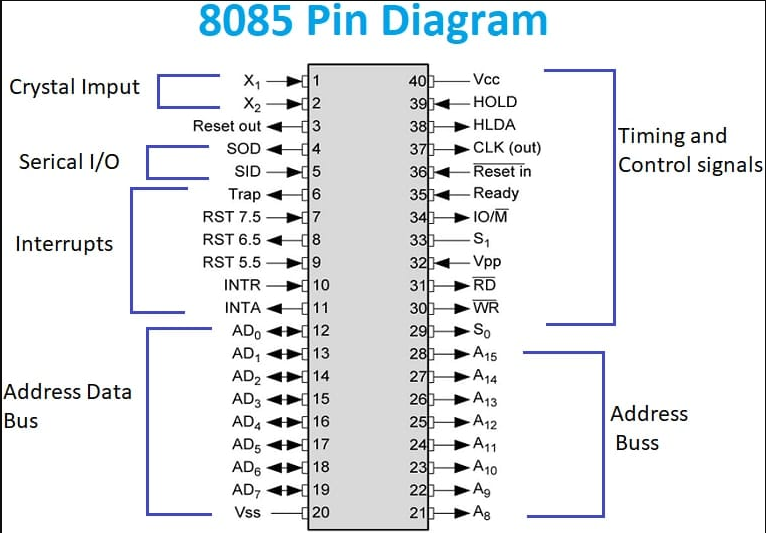
\includegraphics{https://usemynotes.com/wp-content/uploads/2022/10/8085-pin-diagram.jpg}
\caption{}
\end{figure}

\textbf{Explanation of Pin Groups}

\begin{enumerate}
\def\labelenumi{\arabic{enumi}.}
\item
  \textbf{Address Bus (A8-A15):} The upper 8-bits of the 16-bit address
  bus used for addressing memory and I/O devices.
\item
  \textbf{Multiplexed Address/Data Bus (AD0-AD7):} These pins serve two
  functions:

  \begin{itemize}
  \item
    During the first clock state (T1), they carry the lower 8-bits of
    the address.
  \item
    During subsequent clock states, they serve as the data bus for data
    transfer.
  \end{itemize}
\item
  \textbf{Control and Status Signals}

  \begin{itemize}
  \item
    \textbf{ALE (Address Latch Enable):} Indicates that the AD0-AD7
    lines contain a valid address.
  \item
    \textbf{RD (Read):} Indicates a read operation from memory or I/O.
  \item
    \textbf{WR (Write):} Indicates a write operation to memory or I/O.
  \item
    \textbf{IO/M (IO/Memory Select):} Distinguishes between memory (IO/M
    = 0) and I/O (IO/M = 1) operations.
  \item
    \textbf{S0, S1 (Status signals):} These, along with IO/M, indicate
    the type of machine cycle (opcode fetch, memory read, I/O write,
    etc.).
  \end{itemize}
\item
  \textbf{Power Supply and Clock}

  \begin{itemize}
  \item
    \textbf{VCC:} +5V power supply.
  \item
    \textbf{VSS:} Ground (0V).
  \item
    \textbf{X1, X2:} Connections for a crystal or external clock source
    to drive the internal clock generator.
  \item
    \textbf{CLK (OUT):} Clock output signal for synchronizing external
    devices.
  \end{itemize}
\item
  \textbf{Interrupts}

  \begin{itemize}
  \item
    \textbf{TRAP:} Highest priority non-maskable interrupt.
  \item
    \textbf{RST 7.5, RST 6.5, RST 5.5:} Maskable interrupts with
    decreasing priority.
  \item
    \textbf{INTR:} General maskable interrupt.
  \item
    \textbf{INTA:} Interrupt acknowledge signal sent by the 8085.
  \end{itemize}
\item
  \textbf{Serial I/O}

  \begin{itemize}
  \item
    \textbf{SID (Serial Input Data):} Input line for serial data.
  \item
    \textbf{SOD (Serial Output Data):} Output line for serial data.
  \end{itemize}
\item
  \textbf{Reset}

  \begin{itemize}
  \item
    \textbf{RESET IN:} When low, resets the microprocessor, clearing the
    program counter and registers.
  \item
    \textbf{RESET OUT:} Indicates that the microprocessor is being
    reset.
  \end{itemize}
\item
  \textbf{DMA (Direct Memory Access)}

  \begin{itemize}
  \item
    \textbf{HOLD:} Input from a DMA device to request control of buses.
  \item
    \textbf{HLDA:} Acknowledge signal, indicating the 8085 has
    relinquished control of buses.
  \end{itemize}
\end{enumerate}

\hypertarget{211-power-supply-clock--reset-pins}{%
\subsubsection{2.1.1. Power Supply, Clock \& Reset
Pins}\label{211-power-supply-clock--reset-pins}}

Let's delve into the power supply, clock, and reset aspects of the 8085
microprocessor, along with a discussion on common 8085 modules:

\textbf{Power Supply}

\begin{itemize}
\item
  \textbf{Vcc:} The 8085 requires a +5V DC power supply. It is crucial
  to supply a regulated, stable 5V for reliable operation.
\item
  \textbf{Vss:} This is the ground reference (0V) for the power supply.
\item
  \textbf{Current Requirements:} Make sure the power supply can handle
  the current draw of the 8085 as well as other components in your
  system.
\end{itemize}

\textbf{Clock}

\begin{itemize}
\item
  \textbf{X1, X2:} These pins connect to an external crystal oscillator
  circuit. The crystal's resonant frequency determines the fundamental
  clock speed of the 8085.
\item
  \textbf{Frequency:} The 8085 supports frequencies up to 3 MHz or 6 MHz
  (depending on the specific version). You need to choose a crystal with
  double the desired operating frequency due to the internal clock
  divider.
\item
  \textbf{CLK (OUT):} This signal is an output from the 8085 with the
  same frequency as its internal clock. It can serve as a system clock
  for synchronizing other devices.
\end{itemize}

\textbf{Reset}

\begin{itemize}
\item
  \textbf{RESET IN:} This active-low signal is used to reset the 8085.
  When asserted:

  \begin{itemize}
  \item
    The program counter is set to 0000H.
  \item
    Interrupts are disabled.
  \item
    Registers are cleared.
  \end{itemize}
\item
  \textbf{RESET OUT:} This active-high output signal can be used to
  reset other devices in the system during a microprocessor reset.
\end{itemize}

\hypertarget{212-control-and-status-signal-pins}{%
\subsubsection{2.1.2. Control and Status Signal
Pins}\label{212-control-and-status-signal-pins}}

\textbf{Control Signals}

These are signals generated by the 8085 microprocessor to direct and
synchronize operations with memory and I/O devices. Key control signals
include:

\begin{itemize}
\item
  \textbf{RD (Read):}

  \begin{itemize}
  \item
    \textbf{Active Low} (asserted when the signal is low)
  \item
    Issued by the 8085 to indicate that data should be placed on the
    data bus by the selected memory or I/O device.
  \item
    Signals that the microprocessor is reading data.
  \end{itemize}
\item
  \textbf{WR (Write):}

  \begin{itemize}
  \item
    \textbf{Active Low}
  \item
    Issued by the 8085 to indicate that data on the data bus should be
    stored into the selected memory location or I/O port.
  \item
    Signals that the microprocessor is writing data.
  \end{itemize}
\item
  \textbf{IO/M (Input/Output or Memory):}

  \begin{itemize}
  \item
    Used to distinguish between memory and I/O operations.
  \item
    \textbf{IO/M = 1:} Indicates the address bus holds an I/O device
    address.
  \item
    \textbf{IO/M = 0:} Indicates the address bus holds a memory address.
  \end{itemize}
\item
  \textbf{ALE (Address Latch Enable):}

  \begin{itemize}
  \item
    Active high pulse generated at the beginning of a machine cycle.
  \item
    Used to signal external devices to latch the lower 8-bits of the
    address (AD0-AD7) which are multiplexed with the data bus. This
    allows the address to remain stable for use by memory and I/O
    devices.
  \end{itemize}
\end{itemize}

\textbf{Status Signals}

These signals are provided by the 8085 to reflect its current
operational state. Here are the main status signals:

\begin{itemize}
\item
  \textbf{S0, S1:}

  \begin{itemize}
  \item
    These signals indicate the type of operation the 8085 is currently
    performing:

    \begin{longtable}[]{@{}lll@{}}
    \toprule
    S1 & S0 & Operation \\
    \midrule
    \endhead
    0 & 0 & HALT \\
    0 & 1 & Write \\
    1 & 0 & Read \\
    1 & 1 & Opcode Fetch \\
    \bottomrule
    \end{longtable}
  \end{itemize}
\end{itemize}

\textbf{How Control and Status Signals Work Together}

A simplified interaction using these signals would look like this:

\begin{enumerate}
\def\labelenumi{\arabic{enumi}.}
\item
  \textbf{Address Output:} The 8085 places a 16-bit address on the
  address bus and sends a pulse on ALE to latch the lower order address
  bits.
\item
  \textbf{IO/M Signal:} The 8085 sets the IO/M line to indicate whether
  it's a memory or I/O operation.
\item
  \textbf{Read or Write:}

  \begin{itemize}
  \item
    \textbf{Read:} The 8085 asserts the RD line (sets it low). The
    addressed device places data on the data bus for the microprocessor
    to read.
  \item
    \textbf{Write:} The 8085 asserts the WR line (sets it low). Data on
    the data bus is written to the addressed location.
  \end{itemize}
\item
  \textbf{Status:} The 8085 updates S0 and S1 to indicate the type of
  operation that was just performed.
\end{enumerate}

\hypertarget{2121-role-of-ale-signal-in-demultiplexing}{%
\paragraph{2.1.2.1. Role of ALE signal in
Demultiplexing}\label{2121-role-of-ale-signal-in-demultiplexing}}

\textbf{What is the ALE Signal?}

\begin{itemize}
\item
  The ALE signal is a control signal generated by the 8085
  microprocessor.
\item
  It is a positive-going pulse that occurs during the first clock cycle
  (T1 state) of each machine cycle.
\end{itemize}

\textbf{Purpose of the ALE Signal}

The primary function of the ALE signal is to demultiplex the lower-order
address/data bus (AD0-AD7). This bus is shared (multiplexed) to carry
both:

\begin{enumerate}
\def\labelenumi{\arabic{enumi}.}
\item
  \textbf{Lower 8-bits of the Address (during T1 state):} The 8085 needs
  to send out the 16-bit address of a memory location or I/O port. The
  lower 8 bits of the address are carried on lines AD0-AD7.
\item
  \textbf{Data (during subsequent states):} The same lines are used to
  transmit or receive actual data to/from the memory or I/O device.
\end{enumerate}

\textbf{How ALE Demultiplexes the Bus}

\begin{enumerate}
\def\labelenumi{\arabic{enumi}.}
\item
  \textbf{T1 State:}

  \begin{itemize}
  \item
    The ALE signal goes high.
  \item
    The 8085 places the lower 8 bits of the address on lines AD0-AD7.
  \item
    An external latch (usually an 8282 or 8283 octal latch) connected to
    these lines "latches" or captures this address information.
  \end{itemize}
\item
  \textbf{Subsequent States (T2, T3, ...):}

  \begin{itemize}
  \item
    ALE goes low.
  \item
    The lower-order address lines (AD0-AD7) are now free to be used as a
    data bus for transferring data.
  \end{itemize}
\end{enumerate}

\textbf{Diagram}

A simple timing diagram can help visualize this:

\begin{Shaded}
\begin{Highlighting}[]
\NormalTok{          \_\_\_\_\_\_         \_\_\_\_\_\_}
\NormalTok{ALE      |      |\_\_\_\_\_\_\_|      |\_\_\_\_\_\_}
\NormalTok{          \_\_\_\_\_           \_\_\_\_\_}
\NormalTok{AD0{-}AD7  |Addr |\_\_\_\_\_\_\_| Data |\_\_\_\_\_\_\_\_}
\NormalTok{         (T1)      (T2, T3, ...)}
\end{Highlighting}
\end{Shaded}

\textbf{Key Points:}

\begin{itemize}
\item
  The ALE signal is crucial for the 8085 to correctly interface with
  memory and I/O devices.
\item
  The external latch holds the lower order address bits, freeing the
  8085 to continue its fetch or write operation.
\end{itemize}

\hypertarget{213-interrupt-pins}{%
\subsubsection{2.1.3. Interrupt Pins}\label{213-interrupt-pins}}

\textbf{What are Interrupts?}

Interrupts are mechanisms that allow an external device or an internal
event to temporarily halt the currently running program and transfer
control to a special routine called the Interrupt Service Routine (ISR).
ISRs are designed to handle specific events, providing a way to respond
to situations without continuously polling for them.

\textbf{Types of Interrupts in 8085}

The 8085 supports two classes of interrupts:

\begin{enumerate}
\def\labelenumi{\arabic{enumi}.}
\item
  \textbf{Hardware Interrupts:}

  \begin{itemize}
  \item
    Initiated by signals on dedicated interrupt pins of the 8085.
  \item
    Maskable: Can be selectively enabled or disabled using software
    instructions.
  \item
    The 8085 has five hardware interrupts:

    \begin{itemize}
    \item
      \textbf{TRAP (RST 4.5):} Highest priority, non-maskable (cannot be
      disabled). Typically used for critical events like power failures.
    \item
      \textbf{RST 7.5:} Edge-triggered (responds to a signal
      transition). Maskable.
    \item
      \textbf{RST 6.5, RST 5.5:} Level-triggered (responds to a high or
      low level on the pin). Maskable.
    \item
      \textbf{INTR:} General-purpose interrupt. Non-vectored, which
      means the requesting device needs to provide the ISR address.
      Maskable.
    \end{itemize}
  \end{itemize}
\item
  \textbf{Software Interrupts:}

  \begin{itemize}
  \item
    Embedded directly into the program using the RST instructions (RST 0
    through RST 7).
  \item
    These are essentially subroutine calls triggered by software instead
    of hardware.
  \item
    Non-maskable (always execute).
  \end{itemize}
\end{enumerate}

\textbf{Interrupt Handling Process}

Here's a general outline of how the 8085 handles interrupts:

\begin{enumerate}
\def\labelenumi{\arabic{enumi}.}
\item
  \textbf{Interrupt Request:} A device asserts its interrupt pin (or an
  RST instruction is executed).
\item
  \textbf{Acknowledgement:} If interrupts are enabled (using the EI
  instruction), the 8085 finishes its current instruction and sends an
  interrupt acknowledge signal (INTA).
\item
  \textbf{ISR Execution:}

  \begin{itemize}
  \item
    \textbf{Vectored Interrupts (TRAP, RST 7.5, 6.5, 5.5):} The 8085
    automatically jumps to a predefined memory location (vector address)
    associated with the interrupt.
  \item
    \textbf{Non-Vectored Interrupt (INTR):} The interrupting device must
    provide the starting address of its ISR.
  \end{itemize}
\item
  \textbf{Saving State:} The 8085 pushes the current Program Counter
  (PC) onto the stack to preserve the return address.
\item
  \textbf{Executing ISR:} The ISR code is executed to handle the
  specific event.
\item
  \textbf{Return:} Upon completion of the ISR, the RET instruction is
  used to pop the saved PC from the stack, resuming the main program.
\end{enumerate}

\textbf{Key Points}

\begin{itemize}
\item
  \textbf{Interrupt Masking:} The SIM instruction allows you to
  selectively enable or disable maskable interrupts (RST 7.5, 6.5, 5.5).
\item
  \textbf{Interrupt Priority:} If multiple interrupts occur
  simultaneously, they are handled according to fixed priority (TRAP has
  the highest priority).
\item
  \textbf{ISR Placement:} You must carefully place the ISRs in memory,
  especially for vectored interrupts.
\end{itemize}

\hypertarget{214-serial-communication-pins}{%
\subsubsection{2.1.4. Serial Communication
Pins}\label{214-serial-communication-pins}}

The 8085 microprocessor doesn't have a dedicated built-in UART for
serial communication. However, its software can be used to implement
serial communication through its regular input/output pins. Let's
explore this in detail:

\textbf{Serial I/O on the 8085}

The 8085 has two pins dedicated to software-implemented serial
communication:

\begin{itemize}
\item
  \textbf{SID (Serial Input Data):} Used to receive serial data into the
  microprocessor.
\item
  \textbf{SOD (Serial Output Data):} Used to transmit serial data from
  the microprocessor.
\end{itemize}

\textbf{How Serial Communication Works}

Serial communication involves sending or receiving one bit of data at a
time over a single wire. Here's how the 8085 can achieve this:

\begin{enumerate}
\def\labelenumi{\arabic{enumi}.}
\item
  \textbf{Bit Manipulation:} Software instructions are used to set or
  read the voltage level of the SID and SOD pins individually, allowing
  you to transmit and receive bits.
\item
  \textbf{Timing:} Precise timing is crucial in serial communication to
  ensure the receiver correctly interprets transmitted bits. This
  usually involves using delay loops or timers in your 8085 code to
  generate specific intervals.
\item
  \textbf{Protocol:} Serial communication follows standards such as
  RS-232. This means adhering to:

  \begin{itemize}
  \item
    \textbf{Baud Rate:} The speed of transmission (bits per second).
    Sender and receiver must agree on a common baud rate.
  \item
    \textbf{Start/Stop bits:} Special bits to signal the beginning and
    end of a byte transmission.
  \item
    \textbf{Parity (optional):} An error-checking bit.
  \end{itemize}
\end{enumerate}

\textbf{RIM and SIM Instructions}

The 8085 has two special instructions to help in serial communication:

\begin{itemize}
\item
  \textbf{RIM (Read Interrupt Mask):}

  \begin{itemize}
  \item
    Allows checking the status of various interrupt flags including
    status bits for serial data.
  \item
    The Serial Input Data (SID) pin's status can be read using this
    instruction.
  \end{itemize}
\item
  \textbf{SIM (Set Interrupt Mask):}

  \begin{itemize}
  \item
    Used to enable/disable interrupts and also sets the SOD pin's
    status.
  \item
    Setting the SOD bit allows you to transmit data using the SOD pin.
  \end{itemize}
\end{itemize}

\textbf{Example}

A common use case is to implement a simple serial communication program
to send and receive characters to or from a computer terminal. Your code
would typically involve:

\begin{itemize}
\item
  \textbf{Initialization:} Setting up baud rate, parity, etc., using SIM
  and RIM.
\item
  \textbf{Sending Data:}

  \begin{enumerate}
  \def\labelenumi{\arabic{enumi}.}
  \item
    Using SIM to set the SOD bit corresponding to the bit you want to
    send.
  \item
    Introducing an appropriate delay for the required baud rate.
  \item
    Repeat for all bits of the character including start/stop bits.
  \end{enumerate}
\item
  \textbf{Receiving Data:}

  \begin{enumerate}
  \def\labelenumi{\arabic{enumi}.}
  \item
    Sampling the SID pin using RIM at regular intervals matching the
    baud rate.
  \item
    Assembling bits into a byte.
  \end{enumerate}
\end{itemize}

\textbf{Limitations}

\begin{itemize}
\item
  \textbf{Speed:} Software-based serial communication on the 8085 is
  relatively slow and limited by your timing precision.
\item
  \textbf{CPU Overhead:} Handling serial communication through software
  uses up a significant amount of the 8085's processing time.
\end{itemize}

\hypertarget{215-dma-pins}{%
\subsubsection{2.1.5. DMA Pins}\label{215-dma-pins}}

The 8085 microprocessor has the HOLD and HLDA pins, and these signals
are essential for facilitating a limited form of DMA-like behavior.
Here's how it works:

\textbf{How the 8085 Can Mimic DMA Operations}

\begin{enumerate}
\def\labelenumi{\arabic{enumi}.}
\item
  \textbf{DMA Request:} An external peripheral or device (acting as a
  DMA controller of sorts) asserts the HOLD signal, signaling to the
  8085 that it wants to take control of the address and data bus.
\item
  \textbf{CPU Acknowledgement} At the end of its current machine cycle,
  the 8085 will respond by:

  \begin{itemize}
  \item
    Completing any outstanding bus operations.
  \item
    Placing its buses in a high-impedance (tri-stated) mode, effectively
    disconnecting itself from those buses.
  \item
    Asserting the HLDA (Hold Acknowledge) signal, indicating it has
    relinquished control.
  \end{itemize}
\item
  \textbf{Peripheral Takes Over:} The requesting peripheral takes
  control of the address and data buses. It can now perform memory read
  or write operations directly, transferring data without further
  involvement of the 8085 CPU.
\item
  \textbf{Releasing Control:} Once the peripheral is done with the data
  transfer, it releases the HOLD signal.
\item
  \textbf{CPU Regains Control:} The 8085 detects that HOLD is
  de-asserted and subsequently takes back control of the buses, resuming
  its previous operations.
\end{enumerate}

\textbf{Important Considerations}

\begin{itemize}
\item
  \textbf{Not True DMA:} This isn't true DMA in the strictest sense
  since it lacks a fully dedicated DMA controller with its own registers
  and transfer logic. The 8085 CPU is still somewhat involved in the
  process.
\item
  \textbf{Limited Speed:} The CPU needs to actively respond to HOLD and
  HLDA signals, adding some latency and limiting how efficiently large
  blocks of data can be transferred compared to a system with a
  full-fledged DMA controller.
\item
  \textbf{Synchronization:} You need careful synchronization between the
  8085 and the peripheral to ensure they don't clash while attempting to
  access the buses.
\end{itemize}

\textbf{Use Cases}

Even with its limitations, this technique can be useful for devices that
need to transfer data in bursts, like disk drives or high-speed I/O
devices.

\textbf{Example}

Imagine an external device that needs to quickly transfer a block of
data into the 8085's memory. Using the HOLD/HLDA mechanism, this device
can efficiently transfer the data without the CPU needing to actively
read in each individual byte.

\hypertarget{22-block-diagram-of-8085}{%
\subsection{2.2. Block Diagram of 8085}\label{22-block-diagram-of-8085}}

\begin{figure}
\centering
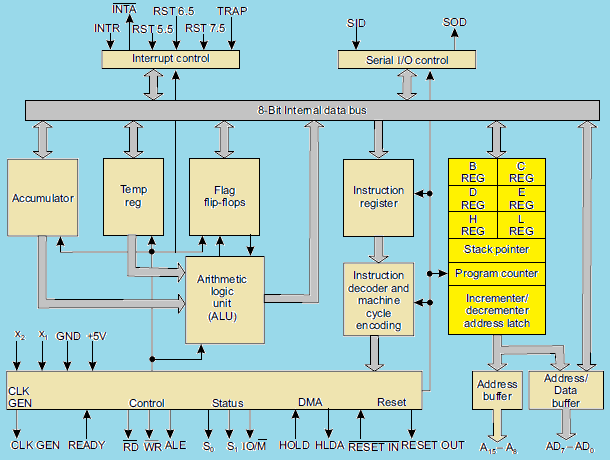
\includegraphics{https://www.electronicsengineering.nbcafe.in/wp-content/uploads/2017/02/8085_architeccher.png}
\caption{}
\end{figure}

\textbf{Key Components and their Functions}

\begin{enumerate}
\def\labelenumi{\arabic{enumi}.}
\item
  \textbf{Accumulator:} An 8-bit register that's central to arithmetic
  and logical operations performed by the ALU.
\item
  \textbf{Arithmetic and Logic Unit (ALU):} Performs arithmetic
  operations (addition, subtraction, etc.) and logical operations (AND,
  OR, NOT, etc.). It sets flags (Carry, Zero, Sign, etc.) based on the
  results.
\item
  \textbf{Temporary Register:} A temporary holding location for data
  used during instruction execution.
\item
  \textbf{Instruction Register:} Holds the currently fetched
  instruction.
\item
  \textbf{Instruction Decoder and Machine Cycle Encoder:} Decodes the
  instruction in the instruction register and generates control signals
  to coordinate the microprocessor's actions during a machine cycle.
\item
  \textbf{Register Array:} Contains six general purpose 8-bit registers
  (B, C, D, E, H, and L), which can be used individually or in pairs
  (BC, DE, HL) for 16-bit operations.
\item
  \textbf{Program Counter (PC):} A 16-bit register that holds the memory
  address of the next instruction to be fetched.
\item
  \textbf{Stack Pointer (SP):} A 16-bit register pointing to the top of
  the stack in memory. The stack is used for storing return addresses of
  subroutines and temporarily storing data.
\item
  \textbf{Timing and Control Unit:} Generates timing and control signals
  for all operations within the microprocessor and synchronizes with
  external devices.
\item
  \textbf{Interrupt Control:} Handles incoming interrupt requests (if
  any), acknowledging them and allowing them to temporarily disrupt the
  current program execution.
\item
  \textbf{Serial I/O Control:} Facilitates serial input and output,
  useful for slower communication with certain types of peripherals.
\item
  \textbf{Address Bus (A8 - A15):} The upper 8-bits of the 16-bit
  address bus, used to send the most significant portion of an address.
\item
  \textbf{Address/Data Bus (AD0 - AD7):} A multiplexed bus. It carries
  the lower 8 bits of an address during the beginning of a machine cycle
  and data during data transfer operations.
\end{enumerate}

\textbf{How it Works (Simplified)}

\begin{enumerate}
\def\labelenumi{\arabic{enumi}.}
\item
  \textbf{Fetch:} The PC provides an address; the instruction is fetched
  from memory and placed into the Instruction Register.
\item
  \textbf{Decode:} The Instruction Decoder decodes the instruction to
  understand what needs to be done.
\item
  \textbf{Execute:} The Control Unit generates signals to coordinate the
  ALU, registers, and other components as they perform the necessary
  operations.
\item
  \textbf{Repeat:} The process continues, fetching and executing
  instructions sequentially.
\end{enumerate}

\hypertarget{221-arithmetic--logic-unit-alu-and-timing--control-unit-cu}{%
\subsubsection{2.2.1. Arithmetic \& Logic Unit (ALU) and Timing \&
Control Unit
(CU)}\label{221-arithmetic--logic-unit-alu-and-timing--control-unit-cu}}

\textbf{Arithmetic and Logic Unit (ALU)}

\begin{itemize}
\item
  \textbf{The Heart of Calculations:} The ALU is responsible for
  performing all the arithmetic and logical operations within the 8085.
\item
  \textbf{Operations:} The 8085's ALU supports the following:

  \begin{itemize}
  \item
    \textbf{Arithmetic:} Addition, subtraction, increment, decrement
  \item
    \textbf{Logical:} AND, OR, XOR, NOT, comparison
  \item
    \textbf{Rotate/Shift:} For bit manipulation.
  \end{itemize}
\item
  \textbf{Inputs and Outputs:}

  \begin{itemize}
  \item
    \textbf{Inputs:} The ALU typically takes two 8-bit operands as
    inputs. One operand usually comes from a temporary register, while
    the other comes from the Accumulator (a special register) or
    directly from the instruction itself.
  \item
    \textbf{Output:} The result of the operation is stored back into the
    Accumulator.
  \end{itemize}
\item
  \textbf{Flags:} The ALU sets or clears various flags in the Flag
  Register based on the result of the operation:

  \begin{itemize}
  \item
    Carry Flag (CY)
  \item
    Zero Flag (Z)
  \item
    Sign Flag (S)
  \item
    Parity Flag (P)
  \item
    Auxiliary Carry Flag (AC)
  \end{itemize}
\end{itemize}

\textbf{Timing and Control Unit}

\begin{itemize}
\item
  \textbf{Conductor of the Orchestra:} The Timing and Control Unit is
  responsible for synchronizing all the operations within the 8085. It
  ensures the correct sequencing of steps for instruction execution and
  communication with other system elements.
\item
  \textbf{Key Functions:}

  \begin{itemize}
  \item
    \textbf{Control signal generation:} Generates control signals (like
    RD, WR, IO/M) for internal components, memory, and I/O devices.
    These signals dictate the direction and timing of data flow.
  \item
    \textbf{Timing Signals:} Creates clock and timing signals for the
    synchronization of the entire system.
  \item
    \textbf{Instruction Execution Coordination:} Governs the fetch,
    decode, and execution stages of instruction processing.
  \item
    \textbf{Interrupt Handling:} Acknowledges and manages the priority
    of interrupts.
  \end{itemize}
\item
  \textbf{Internal Components:}

  \begin{itemize}
  \item
    \textbf{Oscillator:} Generates the fundamental clock signal used as
    a timing reference.
  \item
    \textbf{Control Sequencer:} Logic responsible for producing the
    correct sequence of control signals based on the instructions being
    executed.
  \end{itemize}
\end{itemize}

\textbf{Relationship Between ALU and Timing and Control Unit}

The Timing and Control Unit is the mastermind behind the entire
operation of the 8085. It issues control signals that direct the ALU to
perform specific operations at the appropriate time during instruction
execution. The ALU executes the operations, and its resulting flags
provide information to the Timing and Control Unit, influencing the flow
and decision-making during instruction processing.

\hypertarget{222-registers}{%
\subsubsection{2.2.2. Registers}\label{222-registers}}

\textbf{1. Accumulator (A)}

\begin{itemize}
\item
  \textbf{The Workhorse:} The 8-bit Accumulator is the most heavily used
  register in the 8085. It's involved in a vast majority of arithmetic,
  logical, and I/O operations.
\item
  \textbf{Arithmetic and Logic:} One of the input operands for the ALU
  typically comes from the Accumulator, and the result of operations is
  also stored back into it.
\item
  \textbf{I/O:} Data transferred during input and output operations
  passes through the Accumulator.
\end{itemize}

\textbf{2. Temporary Register (T)}

\begin{itemize}
\item
  \textbf{Hidden Helper:} The Temporary Register is also an 8-bit
  register, but it's not directly accessible to the programmer through
  instructions.
\item
  \textbf{ALU Support:} It serves as a temporary holding space for the
  second operand during some ALU operations.
\item
  \textbf{Indirect Addressing:} The Temporary Register is sometimes
  involved in memory operations where the memory address is specified by
  a register pair (like HL).
\end{itemize}

\textbf{3. Program Counter (PC)}

\begin{itemize}
\item
  \textbf{Keeps Track of Execution:} The PC is a 16-bit register that
  holds the memory address of the next instruction to be fetched and
  executed by the 8085.
\item
  \textbf{Automatic Incrementing:} After fetching an instruction, the PC
  automatically increments to point to the next sequential instruction
  in memory.
\item
  \textbf{Control Flow Changes:} Instructions like JUMP and CALL modify
  the Program Counter to change the execution flow of your program.
\end{itemize}

\textbf{4. Stack Pointer (SP)}

\begin{itemize}
\item
  \textbf{LIFO Structure:} The Stack Pointer is a 16-bit register that
  points to the current top of the stack in memory. The stack is a
  Last-In, First-Out data structure.
\item
  \textbf{PUSH and POP:} Instructions like PUSH and POP add data to or
  remove data from the top of the stack respectively, with the SP
  automatically adjusting.
\item
  \textbf{Subroutine Calls and Interrupts:} The stack is used to
  temporarily store the return address during subroutine calls (CALL)
  and during interrupt handling. This ensures the program can return to
  the correct place when the subroutine or interrupt service routine
  finishes.
\end{itemize}

\textbf{5. Register Array (B, C, D, E, H, L)}

\begin{itemize}
\item
  \textbf{General Purpose Registers:} These are six 8-bit registers that
  can be used individually or in pairs:

  \begin{itemize}
  \item
    BC (16-bit)
  \item
    DE (16-bit)
  \item
    HL (16-bit)
  \end{itemize}
\item
  \textbf{Data Storage:} Used to temporarily hold data during program
  execution.
\item
  \textbf{Memory Addressing:} The HL register pair, in particular, is
  often used to hold 16-bit memory addresses for addressing data in
  memory.
\end{itemize}

\textbf{Key Points}

\begin{itemize}
\item
  \textbf{Limited Registers:} The 8085 has a limited set of registers,
  so programmers need to manage register use efficiently.
\item
  \textbf{Special Roles:} Registers like the Accumulator, Stack Pointer,
  and Program Counter have very specific roles, while the other
  general-purpose registers provide more flexibility.
\end{itemize}

\hypertarget{223-instruction-register-instruction-decoder-and-machine-cycle-encoder}{%
\subsubsection{2.2.3. Instruction Register, Instruction Decoder, and
Machine Cycle
Encoder}\label{223-instruction-register-instruction-decoder-and-machine-cycle-encoder}}

\textbf{1. Instruction Register (IR)}

\begin{itemize}
\item
  \textbf{Purpose:} The Instruction Register serves as a temporary
  holding area for the current instruction being executed by the 8085.
\item
  \textbf{Operation:} When an instruction is fetched from memory, it is
  placed into the Instruction Register.
\item
  \textbf{Connection:} The IR is directly connected to the internal data
  bus of the 8085.
\end{itemize}

\textbf{2. Instruction Decoder}

\begin{itemize}
\item
  \textbf{Purpose:} The Instruction Decoder is a complex combinatorial
  circuit that analyzes the instruction currently in the Instruction
  Register. Its main function is to determine the nature of the
  instruction and figure out what actions the 8085 needs to take to
  execute it.
\item
  \textbf{Decoding Process:}

  \begin{itemize}
  \item
    Breaks down the instruction's opcode (the part that specifies the
    operation).
  \item
    Identifies any operands or addressing modes involved.
  \item
    Generates internal control signals to orchestrate the various steps
    required to execute the specific instruction.
  \end{itemize}
\end{itemize}

\textbf{3. Machine Cycle Encoder}

\begin{itemize}
\item
  \textbf{Purpose:} The Machine Cycle Encoder is responsible for
  generating the timing and control signals necessary to carry out the
  steps required for instruction execution.
\item
  \textbf{Machine Cycles:} Instructions in the 8085 consist of one or
  more machine cycles. Examples include:

  \begin{itemize}
  \item
    Opcode Fetch cycle: To retrieve the instruction from memory.
  \item
    Memory Read cycle: To read data from memory
  \item
    Memory Write cycle: To write data to memory
  \item
    I/O Read/Write cycles: To communicate with input/output devices
  \end{itemize}
\item
  \textbf{Control Signals:} The Machine Cycle Encoder produces control
  signals to direct the flow of data, activate specific registers or the
  ALU, and interface with the memory and I/O systems.
\end{itemize}

\textbf{How They Work Together}

\begin{enumerate}
\def\labelenumi{\arabic{enumi}.}
\item
  \textbf{Fetch:} The opcode of an instruction is fetched from memory
  and placed into the Instruction Register.
\item
  \textbf{Decode:} The Instruction Decoder analyzes the opcode, figuring
  out what operation needs to be performed and any data locations
  involved.
\item
  \textbf{Execute:} The Machine Cycle Encoder generates the necessary
  sequence of control signals to carry out the instruction, potentially
  over multiple machine cycles. These signals direct the actions of the
  8085's internal components.
\end{enumerate}

\hypertarget{224-the-flag-register}{%
\subsubsection{2.2.4. The Flag Register}\label{224-the-flag-register}}

The Flag register in the 8085 is an 8-bit register, with only 5 bits
actively used as flags. These flags act as individual flip-flops that
are set (1) or reset (0) to reflect specific conditions arising from
arithmetic, logical, and other operations performed by the ALU
(Arithmetic and Logic Unit).

\textbf{The 5 Flags:}

\begin{enumerate}
\def\labelenumi{\arabic{enumi}.}
\item
  \textbf{Sign Flag (S):}

  \begin{itemize}
  \item
    Set (1) if the result of an operation is negative (the Most
    Significant Bit, or MSB, of the result is 1).
  \item
    Reset (0) if the result is positive.
  \end{itemize}
\item
  \textbf{Zero Flag (Z):}

  \begin{itemize}
  \item
    Set (1) if the result of an operation is zero.
  \item
    Reset (0) if the result is not zero.
  \end{itemize}
\item
  \textbf{Auxiliary Carry Flag (AC):}

  \begin{itemize}
  \item
    Set (1) if there is a carry-out from the lower nibble (lower 4 bits)
    into the upper nibble (upper 4 bits) of a result.
  \item
    Used primarily in instructions that perform decimal arithmetic.
  \end{itemize}
\item
  \textbf{Parity Flag (P):}

  \begin{itemize}
  \item
    Set (1) if the result has even parity (contains an even number of
    1s).
  \item
    Reset (0) if the result has odd parity.
  \end{itemize}
\item
  \textbf{Carry Flag (CY):}

  \begin{itemize}
  \item
    Set (1) if there is a carry-out from the most significant bit (MSB)
    of a result during addition, or a borrow during subtraction.
  \item
    Reset (0) otherwise.
  \end{itemize}
\end{enumerate}

\textbf{How the Flags are Used:}

\begin{itemize}
\item
  \textbf{Conditional Jumps:} Instructions like JZ (Jump if Zero), JNZ
  (Jump if Not Zero), JC (Jump if Carry), etc. use the status of these
  flags to determine whether to branch to different parts of the
  program.
\item
  \textbf{Decision Making:} The processor can examine flag states to
  modify calculations or behaviors based on previous operations.
\end{itemize}

\textbf{Example:}

\begin{Shaded}
\begin{Highlighting}[]
\NormalTok{; Assume the accumulator (A) holds the value 50}
\NormalTok{SUB B  ; Subtract the value in register B from the accumulator}
\NormalTok{JZ LABEL  ; If the result is zero, jump to the code section marked as LABEL}
\end{Highlighting}
\end{Shaded}

\hypertarget{225-bus-organization}{%
\subsubsection{2.2.5. Bus Organization}\label{225-bus-organization}}

A bus, in a microprocessor system, is a collection of signal lines used
to transfer data between the CPU and other components (memory, I/O
devices). The 8085 microprocessor has a well-defined bus organization
consisting of three main buses:

\begin{itemize}
\item
  \textbf{Address Bus}

  \begin{itemize}
  \item
    \textbf{Unidirectional} (data flows from the microprocessor
    outwards)
  \item
    \textbf{16-bit wide} (Can address up to 64KB of memory)
  \item
    Carries the memory address of the location the microprocessor wants
    to access.
  \end{itemize}
\item
  \textbf{Data Bus}

  \begin{itemize}
  \item
    \textbf{Bidirectional} (data can flow in both directions)
  \item
    \textbf{8-bit wide} (carries 8 bits of data at a time)
  \item
    Used to transfer both data and instructions between the
    microprocessor and memory/IO.
  \end{itemize}
\item
  \textbf{Control Bus}

  \begin{itemize}
  \item
    \textbf{Mixture of unidirectional and bidirectional lines}
  \item
    Consists of various control signals like:

    \begin{itemize}
    \item
      \textbf{RD (Read):} Indicates the CPU wants to read data from
      memory or an I/O port.
    \item
      \textbf{WR (Write):} Indicates the CPU wants to write data to
      memory or an I/O port.
    \item
      \textbf{IO/M:} Distinguishes between a memory operation (IO/M = 0)
      or I/O operation (IO/M = 1).
    \end{itemize}
  \end{itemize}
\end{itemize}

\textbf{Simplified Diagram}

\begin{Shaded}
\begin{Highlighting}[]
\NormalTok{        +{-}{-}{-}{-}{-}{-}{-}{-}{-}{-}{-}{-}{-}{-}{-}{-}{-}{-}{-}{-}+}
\NormalTok{        |    Microprocessor  |}
\NormalTok{        |       8085         |}
\NormalTok{        +{-}{-}{-}{-}{-}{-}{-}{-}{-}{-}{-}{-}{-}{-}{-}{-}{-}{-}{-}{-}+}
\NormalTok{               |       |}
\NormalTok{               | (Address Bus)}
\NormalTok{               |       |}
\NormalTok{   +{-}{-}{-}{-}{-}{-}{-}{-}{-}{-}{-}+{-}{-}{-}{-}{-}{-}{-}{-}{-}{-}{-}+{-}{-}{-}{-}{-}{-}{-}{-}{-}{-}{-}+}
\NormalTok{   | Memory    | I/O Ports | Other     |}
\NormalTok{   |           |           | Devices   |}
\NormalTok{   +{-}{-}{-}{-}{-}{-}{-}{-}{-}{-}{-}+{-}{-}{-}{-}{-}{-}{-}{-}{-}{-}{-}+{-}{-}{-}{-}{-}{-}{-}{-}{-}{-}{-}+}
\NormalTok{               |       |}
\NormalTok{               | (Data Bus)}
\NormalTok{               |       |}
\NormalTok{      \textless{}{-}{-}{-}{-}{-}{-}{-}{-}+{-}{-}{-}{-}{-}{-}{-}{-}{-}\textgreater{}}
\NormalTok{               | (Control Bus)}
\end{Highlighting}
\end{Shaded}

\textbf{Explanation}

\begin{enumerate}
\def\labelenumi{\arabic{enumi}.}
\item
  \textbf{Microprocessor:} The 8085 is the heart of the system,
  initiating and controlling data transfers.
\item
  \textbf{Address Bus} : Used by the microprocessor to specify the
  location in memory or I/O it wants to communicate with.
\item
  \textbf{Data Bus:} The actual data or instructions are transferred
  over the data bus.
\item
  \textbf{Control Bus:} The microprocessor uses the control bus to send
  signals that coordinate the timing and direction of data transfers.
\end{enumerate}

\textbf{Key Points}

\begin{itemize}
\item
  \textbf{Multiplexing:} The 8085 multiplexes the lower 8-bits of the
  address bus (AD0-AD7) with the data bus (D0-D7) to reduce pin count.
  This means the same set of lines carries both address bits (at the
  beginning of a cycle) and data.
\item
  \textbf{Interfacing:} The bus organization dictates how you connect
  and control memory chips and I/O devices within an 8085-based system.
\end{itemize}

\hypertarget{23-working-of-the-8085}{%
\subsection{2.3. Working of the 8085}\label{23-working-of-the-8085}}

\hypertarget{231-memory-interfacing}{%
\subsubsection{2.3.1. Memory Interfacing}\label{231-memory-interfacing}}

\textbf{Key Concepts}

\begin{itemize}
\item
  \textbf{Address Bus:} The 8085 has a 16-bit address bus (A0-A15),
  allowing it to address up to 64KB of memory.
\item
  \textbf{Data Bus:} The 8085 has an 8-bit data bus (D0-D7) for
  transferring data between the microprocessor and memory.
\item
  \textbf{Control Signals:} Control signals (like RD, WR, IO/M) are
  crucial for indicating the direction of data flow and the type of
  operation.
\end{itemize}

\textbf{Memory Organization}

\begin{itemize}
\item
  \textbf{Memory Map:} The 64KB address space of the 8085 is often
  divided into portions for specific purposes:

  \begin{itemize}
  \item
    \textbf{ROM (Read-Only Memory):} Used to store the program
    instructions, which usually reside at the lower end of the address
    space.
  \item
    \textbf{RAM (Random Access Memory):} Used for storing variables,
    temporary data, and the stack, which often starts at the higher end
    of the address space.
  \end{itemize}
\item
  \textbf{I/O Mapped I/O:} Some address space can be reserved for
  interfacing with input/output devices.
\end{itemize}

\begin{figure}
\centering
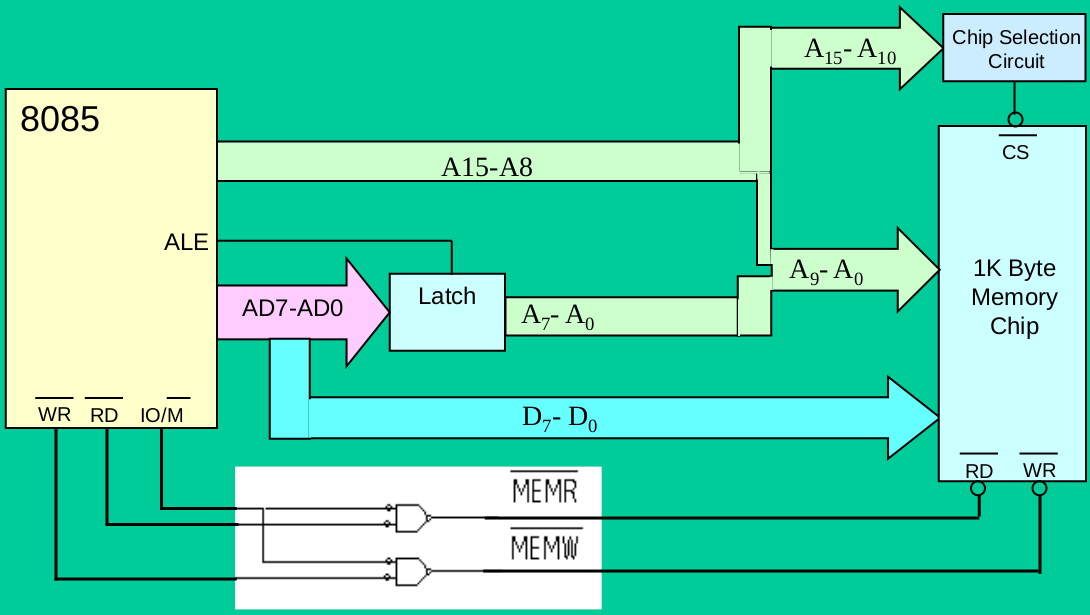
\includegraphics{/home/milav/Codes/MPMC/assets/imgs/8085_Memory_Interfacing.png}
\caption{}
\end{figure}

\textbf{Memory Read Cycle}

\begin{enumerate}
\def\labelenumi{\arabic{enumi}.}
\item
  \textbf{Address Output:} The 8085 places the 16-bit address of the
  memory location it wants to read on the address bus.
\item
  \textbf{Control Signals:}

  \begin{itemize}
  \item
    The IO/M signal is set low (IO/M = 0), indicating a memory
    operation.
  \item
    The RD (Read) signal is asserted (set low) to signal a read
    operation.
  \end{itemize}
\item
  \textbf{Data Transfer:} The addressed memory chip places the data from
  the specified location onto the data bus.
\item
  \textbf{Data Latch:} The 8085 microprocessor reads the data from the
  data bus and stores it internally (likely in a register).
\end{enumerate}

\textbf{Memory Write Cycle}

\begin{enumerate}
\def\labelenumi{\arabic{enumi}.}
\item
  \textbf{Address Output:} Similar to a read cycle, the 8085 places the
  16-bit memory address on the address bus.
\item
  \textbf{Data Output:} The 8085 places the data it intends to write
  onto the data bus.
\item
  \textbf{Control Signals:}

  \begin{itemize}
  \item
    IO/M is set low (IO/M = 0) to indicate a memory operation.
  \item
    The WR (Write) signal is asserted (set low) to signal a write
    operation.
  \end{itemize}
\item
  \textbf{Data Storage:} The addressed memory location stores the data
  from the data bus.
\end{enumerate}

\textbf{Memory Interfacing Techniques}

\begin{itemize}
\item
  \textbf{Address Decoding:} To interface multiple memory (and I/O)
  devices, you'll need address decoding logic. Using gates and logic
  circuits, you can ensure that the correct memory chip or I/O device is
  activated based on the address on the address bus.
\item
  \textbf{Multiplexing:} The lower 8-bits of the address bus (A0-A7) are
  multiplexed with the data bus (D0-D7). The ALE signal is used to latch
  the address and demultiplex it.
\end{itemize}

\hypertarget{232-demultiplexing-of-lower-order-address-bus--data-bus}{%
\subsubsection{2.3.2. Demultiplexing of Lower Order Address Bus \& Data
Bus}\label{232-demultiplexing-of-lower-order-address-bus--data-bus}}

\textbf{Why Demultiplexing is Needed}

The Intel 8085 utilizes a multiplexed address/data bus to reduce the
number of pins required. The lower 8 lines (AD0-AD7) carry two types of
information:

\begin{enumerate}
\def\labelenumi{\arabic{enumi}.}
\item
  \textbf{Address (during T1 state):} During the first clock cycle of a
  machine cycle, these lines hold the lower 8 bits of a 16-bit memory or
  I/O address.
\item
  \textbf{Data (during subsequent states):} In the remaining clock
  cycles, those same lines transmit or receive the actual data being
  sent to or from a memory location or I/O device.
\end{enumerate}

\textbf{Demultiplexing Process}

Demultiplexing is the process of separating the address and data
information so the 8085 and external devices can operate correctly.
Here's how it's achieved:

\begin{enumerate}
\def\labelenumi{\arabic{enumi}.}
\item
  \textbf{The ALE Signal:} During the first clock cycle (T1), the 8085
  asserts the ALE (Address Latch Enable) control signal. This signal
  goes high.
\item
  \textbf{External Latch:} An external latch circuit (e.g., 8282 or
  74LS373 octal latch) is connected to the AD0-AD7 lines. When the ALE
  signal goes high, this latch captures and holds the lower 8 bits of
  the address.
\item
  \textbf{Address Decoded:} The latched lower-order address bits, along
  with the higher-order address bits (A8-A15), provide the complete
  16-bit address for memory or I/O devices.
\item
  \textbf{Data Bus Freed:} After the T1 state, the ALE signal goes low.
  The AD0-AD7 lines are now free to be used as a data bus for the
  remainder of the machine cycle.
\end{enumerate}

\textbf{Diagram}

\begin{figure}
\centering
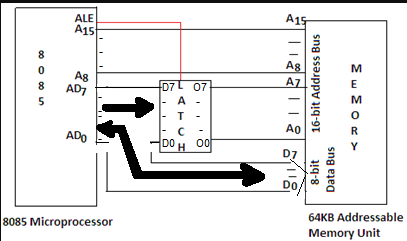
\includegraphics{https://care4you.in/wp-content/uploads/2022/02/de-multiplexing.png}
\caption{}
\end{figure}

\textbf{Key Points}

\begin{itemize}
\item
  Demultiplexing enables the 8085 to interface with memory and I/O
  devices correctly by separating the address and data functions of the
  same physical bus lines.
\item
  The ALE signal plays a crucial role in timing the latching of address
  information.
\end{itemize}

\hypertarget{233-instruction-fetching-decoding-and-execution}{%
\subsubsection{2.3.3. Instruction Fetching, Decoding and
Execution}\label{233-instruction-fetching-decoding-and-execution}}

\textbf{Instruction Fetching}

\begin{enumerate}
\def\labelenumi{\arabic{enumi}.}
\item
  \textbf{Program Counter (PC):} The PC, a 16-bit register, holds the
  memory address of the next instruction to be fetched.
\item
  \textbf{Memory Address Register (MAR):} The contents of the PC are
  copied into the MAR.
\item
  \textbf{Memory Read:} The 8085's control unit sends a read signal to
  the memory, and the instruction code at the address specified by the
  MAR is placed on the data bus.
\item
  \textbf{Instruction Register (IR):} The instruction code is
  transferred from the data bus to the Instruction Register.
\item
  \textbf{PC Increment:} The PC is incremented to point to the next
  instruction in memory.
\end{enumerate}

\textbf{Instruction Decoding}

\begin{enumerate}
\def\labelenumi{\arabic{enumi}.}
\item
  \textbf{Instruction Decoder:} The instruction code in the IR is
  interpreted by the 8085's instruction decoder circuitry. It identifies
  the specific operation to be performed (opcode) and the operands
  involved.
\item
  \textbf{Control Signals:} The instruction decoder generates
  appropriate control signals to coordinate the upcoming execution.
  These signals control the flow of data within the 8085, directing the
  ALU, registers, and the timing of operations.
\end{enumerate}

\textbf{Instruction Execution}

The execution phase varies significantly depending on the specific
instruction. Here's a general breakdown of the kinds of steps involved:

\begin{itemize}
\item
  \textbf{Operand Fetching:} If the instruction uses operands (data),
  additional machine cycles may be involved in fetching these from
  either:

  \begin{itemize}
  \item
    \textbf{Registers:} Accessed directly within the microprocessor.
  \item
    \textbf{Memory:} The MAR is loaded with the memory address of the
    operand, and another memory read operation is performed.
  \end{itemize}
\item
  \textbf{ALU Operations:} For arithmetic or logical instructions, the
  ALU is engaged to perform the required calculation or comparison.
\item
  \textbf{Result Storage:} The results of an operation may be stored in:

  \begin{itemize}
  \item
    \textbf{Accumulator:} A special register within the 8085.
  \item
    \textbf{Other General-Purpose Registers}
  \item
    \textbf{Memory:} Another memory write operation might be needed.
  \end{itemize}
\item
  \textbf{Update Status Flags:} The ALU sets flags (Zero, Carry, Sign,
  etc.) to reflect the results of its operations, which can be used for
  conditional branching later.
\end{itemize}

\textbf{Example: ADD B Instruction}

Let's assume the instruction "ADD B" (add the value in register B to the
accumulator) is being executed:

\begin{enumerate}
\def\labelenumi{\arabic{enumi}.}
\item
  \textbf{Fetch:} The opcode for ADD B is fetched from memory and placed
  in the IR.
\item
  \textbf{Decode:} The instruction decoder determines that this is an
  addition operation and that the operand is in register B.
\item
  \textbf{Execute:}

  \begin{itemize}
  \item
    The contents of register B are fetched.
  \item
    The ALU performs the addition between the accumulator's current
    value and the value from register B.
  \item
    The result is stored back into the accumulator.
  \end{itemize}
\end{enumerate}

\hypertarget{2331-instruction-fetching}{%
\paragraph{2.3.3.1. Instruction
Fetching}\label{2331-instruction-fetching}}

\begin{enumerate}
\def\labelenumi{\arabic{enumi}.}
\item
  \textbf{Program Counter (PC):} The PC, a 16-bit register, holds the
  memory address of the next instruction to be fetched.
\item
  \textbf{Memory Address Register (MAR):} The contents of the PC are
  copied into the MAR.
\item
  \textbf{Memory Read:} The 8085's control unit sends a read signal to
  the memory, and the instruction code at the address specified by the
  MAR is placed on the data bus.
\item
  \textbf{Instruction Register (IR):} The instruction code is
  transferred from the data bus to the Instruction Register.
\item
  \textbf{PC Increment:} The PC is incremented to point to the next
  instruction in memory.
\end{enumerate}

\hypertarget{2332-instruction-decoding}{%
\paragraph{2.3.3.2. Instruction
Decoding}\label{2332-instruction-decoding}}

\begin{enumerate}
\def\labelenumi{\arabic{enumi}.}
\item
  \textbf{Instruction Decoder:} The instruction code in the IR is
  interpreted by the 8085's instruction decoder circuitry. It identifies
  the specific operation to be performed (opcode) and the operands
  involved.
\item
  \textbf{Control Signals:} The instruction decoder generates
  appropriate control signals to coordinate the upcoming execution.
  These signals control the flow of data within the 8085, directing the
  ALU, registers, and the timing of operations.
\end{enumerate}

\hypertarget{2333-instruction-execution}{%
\paragraph{2.3.3.3. Instruction
Execution}\label{2333-instruction-execution}}

The execution phase varies significantly depending on the specific
instruction. Here's a general breakdown of the kinds of steps involved:

\begin{itemize}
\item
  \textbf{Operand Fetching:} If the instruction uses operands (data),
  additional machine cycles may be involved in fetching these from
  either:

  \begin{itemize}
  \item
    \textbf{Registers:} Accessed directly within the microprocessor.
  \item
    \textbf{Memory:} The MAR is loaded with the memory address of the
    operand, and another memory read operation is performed.
  \end{itemize}
\item
  \textbf{ALU Operations:} For arithmetic or logical instructions, the
  ALU is engaged to perform the required calculation or comparison.
\item
  \textbf{Result Storage:} The results of an operation may be stored in:

  \begin{itemize}
  \item
    \textbf{Accumulator:} A special register within the 8085.
  \item
    \textbf{Other General-Purpose Registers}
  \item
    \textbf{Memory:} Another memory write operation might be needed.
  \end{itemize}
\item
  \textbf{Update Status Flags:} The ALU sets flags (Zero, Carry, Sign,
  etc.) to reflect the results of its operations, which can be used for
  conditional branching later.
\end{itemize}

\hypertarget{2334-example-add-b-instruction}{%
\paragraph{2.3.3.4. Example: ADD B
Instruction}\label{2334-example-add-b-instruction}}

Let's assume the instruction "ADD B" (add the value in register B to the
accumulator) is being executed:

\begin{enumerate}
\def\labelenumi{\arabic{enumi}.}
\item
  \textbf{Fetch:} The opcode for ADD B is fetched from memory and placed
  in the IR.
\item
  \textbf{Decode:} The instruction decoder determines that this is an
  addition operation and that the operand is in register B.
\item
  \textbf{Execute:}

  \begin{itemize}
  \item
    The contents of register B are fetched.
  \item
    The ALU performs the addition between the accumulator's current
    value and the value from register B.
  \item
    The result is stored back into the accumulator.
  \end{itemize}
\end{enumerate}

\hypertarget{24-microprocessor-vs-microcontroller}{%
\subsection{2.4. Microprocessor vs.
Microcontroller}\label{24-microprocessor-vs-microcontroller}}

\textbf{Core Distinction}

\begin{itemize}
\item
  \textbf{Microprocessor:} A Central Processing Unit (CPU) on a chip.
  It's the "brain" of a computer system, designed for general-purpose
  computing and requires external components to form a functional
  system.
\item
  \textbf{Microcontroller:} A self-contained "computer-on-a-chip." It
  integrates a CPU, memory, and peripherals, optimized for embedded
  control applications.
\end{itemize}

\textbf{Key Features}

\begin{longtable}[]{@{}lll@{}}
\toprule
Feature & Microprocessor & Microcontroller \\
\midrule
\endhead
\textbf{System Design} & Core of a complex system & Often the entire
system \\
\textbf{Complexity} & Less complex internally & More complex internally
due to integrated components \\
\textbf{Instruction Set} & Larger, versatile instruction set for diverse
operations & Smaller, tailored instruction set for specific
applications \\
\textbf{Memory} & External RAM, ROM, flash required & On-chip RAM, ROM,
often with flash memory \\
\textbf{Peripherals} & Requires external interfacing & Built-in
peripherals (timers, ADCs, DACs, communication ports) \\
\textbf{Power Consumption} & Generally higher power consumption &
Optimized for low power operation \\
\textbf{Cost} & Generally lower cost & Can be higher due to integrated
components \\
\textbf{Flexibility} & Highly flexible for various tasks & More
specialized, less adaptable to diverse use cases \\
\textbf{Applications} & Desktop computers, laptops, servers, complex
systems & Embedded systems, appliances, medical devices, IoT devices \\
\textbf{Examples} & Intel Core Series, AMD Ryzen, IBM Power & Atmel AVR,
PIC, ARM Cortex-M, Texas Instruments MSP430 \\
\bottomrule
\end{longtable}

\textbf{Additional Considerations}

\begin{itemize}
\item
  \textbf{Programming:} Microcontrollers often require more low-level
  knowledge of hardware for efficient programming.
\item
  \textbf{Performance:} Microprocessors generally excel in raw
  computational performance, while microcontrollers prioritize power
  efficiency and responsiveness.
\item
  \textbf{Bit Handling:} Microcontrollers frequently offer better
  support for bit-level operations on I/O pins.
\end{itemize}

\textbf{Illustrative Analogy}

Imagine building a custom robot:

\begin{itemize}
\item
  \textbf{Microprocessor:} Like buying the high-performance brain for
  your robot. You'd still need to buy sensors, motors, a power supply,
  and design the entire body.
\item
  \textbf{Microcontroller:} Like buying a pre-assembled robot kit with a
  basic brain, sensors, and motors. You focus on programming behavior,
  potentially adding some external components if needed.
\end{itemize}

\textbf{When to Choose Which}

\begin{itemize}
\item
  \textbf{Microprocessor:} Need high computational power, flexibility
  for a variety of tasks, or working with large amounts of data.
\item
  \textbf{Microcontroller:} Self-contained solution, low-power,
  real-time control, or cost-sensitive applications are priorities.
\end{itemize}

\hypertarget{3-unit-iii-microcontroller-architecture}{%
\section{3. Unit III: Microcontroller
Architecture}\label{3-unit-iii-microcontroller-architecture}}

\hypertarget{31-general-block-diagram-of-a-microcontroller}{%
\subsection{3.1. General Block Diagram of a
Microcontroller}\label{31-general-block-diagram-of-a-microcontroller}}

\begin{figure}
\centering
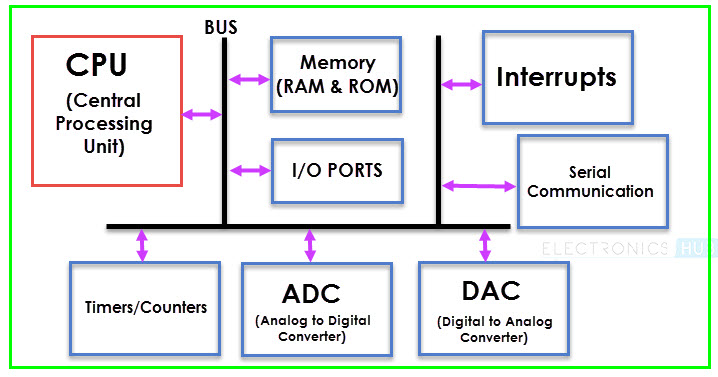
\includegraphics{/home/milav/Codes/MPMC/assets/imgs/181001_MCU_Question_Bank_Solved_html_87f3259625e90fef.png}
\caption{}
\end{figure}

\textbf{Understanding the Core Components and Their Interconnections}

\begin{itemize}
\item
  \textbf{CPU (Central Processing Unit)}

  \begin{itemize}
  \item
    \textbf{ALU (Arithmetic Logic Unit):} The heart of calculations and
    logic operations. Performs arithmetic (addition, subtraction, etc.),
    logical (AND, OR, NOT) comparisons, and data manipulation.
  \item
    \textbf{Control Unit (CU):} The manager that fetches instructions
    from memory, decodes them, and generates control signals to
    orchestrate the actions of all components within the
    microcontroller.
  \item
    \textbf{Registers:} Small, incredibly fast memory units built into
    the CPU for temporarily storing data, instructions, and intermediate
    results.
  \end{itemize}
\item
  \textbf{Memory}

  \begin{itemize}
  \item
    \textbf{ROM (Read-Only Memory):} Non-volatile memory used to
    permanently store the microcontroller's firmware (program code) and
    essential data.
  \item
    \textbf{RAM (Random Access Memory):} Volatile memory for storing
    temporary data and variables used while the microcontroller is
    running a program.
  \item
    \textbf{Flash Memory:} In modern microcontrollers, flash memory
    often replaces traditional ROM for its flexibility, offering
    reprogrammable program memory.
  \end{itemize}
\item
  \textbf{I/O Ports (Input/Output Ports):} Versatile pins that can be
  configured as either inputs or outputs.

  \begin{itemize}
  \item
    \textbf{Inputs:} Connect to external sensors, switches, keypads, and
    other input devices that provide information to the microcontroller.
  \item
    \textbf{Outputs:} Drive LEDs, displays, motors, actuators and other
    devices for interacting with the external world.
  \end{itemize}
\item
  \textbf{Bus System:} A communication network of wires connecting the
  CPU, memory, I/O ports, and other components.

  \begin{itemize}
  \item
    \textbf{Address Bus:} Carries memory addresses to specify locations
    for data transfer.
  \item
    \textbf{Data Bus:} Transfers data between the various components.
  \item
    \textbf{Control Bus:} Transmits control signals (read/write, timing,
    etc.) to synchronize operations.
  \end{itemize}
\item
  \textbf{Timers/Counters:} Specialized modules for:

  \begin{itemize}
  \item
    \textbf{Generating Accurate Time Delays:} Essential for controlling
    the timing of operations.
  \item
    \textbf{Counting External Events:} Measuring frequencies, pulse
    widths, and more.
  \item
    \textbf{Output Waveform Generation:} Like Pulse Width Modulation
    (PWM) for motor control, dimming LEDs, etc.
  \end{itemize}
\item
  \textbf{Serial Port:} Facilitates communication with other devices
  using standard protocols like:

  \begin{itemize}
  \item
    \textbf{UART:} Universal Asynchronous Receiver/Transmitter (common
    for simple serial communication).
  \item
    \textbf{SPI, I2C:} For interfacing with various sensors and
    peripherals.
  \end{itemize}
\item
  \textbf{Interrupts:} Signals that allow the microcontroller to respond
  to high-priority events immediately

  \begin{itemize}
  \item
    \textbf{External Interrupts:} Triggered by changes on input pins
    (e.g., button presses).
  \item
    \textbf{Internal Interrupts:} Generated by timers, ADCs, or other
    peripherals.
  \end{itemize}
\item
  \textbf{ADC (Analog to Digital Converter):} Converts incoming analog
  signals (e.g., from temperature sensors) into digital values that the
  CPU can process.
\item
  \textbf{DAC (Digital to Analog Converter):} Transforms digital data
  from the CPU into analog signals useful for driving devices like
  speakers or creating smooth control voltages.
\item
  \textbf{On-Chip Oscillator:} Provides the internal clock signal that
  drives the microcontroller's timing.
\item
  \textbf{Special Function Registers (SFRs):} Registers dedicated to
  controlling the configuration and operation of the microcontroller's
  peripherals.
\end{itemize}

\hypertarget{32-pin-diagram-of-8051}{%
\subsection{3.2. Pin Diagram of 8051}\label{32-pin-diagram-of-8051}}

The following image shows the 8051 Microcontroller Pin Diagram with
respect to a 40 -- pin Dual In-line Package (DIP).

\textbf{Pins 1 -- 8 (PORT 1):}

\begin{itemize}
\item
  Pins 1 to 8 are the PORT 1 Pins of 8051. PORT 1 Pins consists of 8 --
  bit bidirectional Input / Output Port with internal pull -- up
  resistors. In older 8051 Microcontrollers, PORT 1 doesn't serve any
  additional purpose but just 8 -- bit I/O PORT.
\item
  In some of the newer 8051 Microcontrollers, few PORT 1 Pins have dual
  functions. P1.0 and P1.1 act as Timer 2 and Timer 2 Trigger Input
  respectively.
\item
  P1.5, P1.6 and P1.7 act as In-System Programming Pins i.e. MOSI, MISO
  and SCK respectively.
\end{itemize}

\textbf{Pin 9 (RST):} Pin 9 is the Reset Input Pin. It is an active HIGH
Pin i.e. if the RST Pin is HIGH for a minimum of two machine cycles, the
microcontroller will be reset. During this time, the oscillator must be
running.

\begin{figure}
\centering
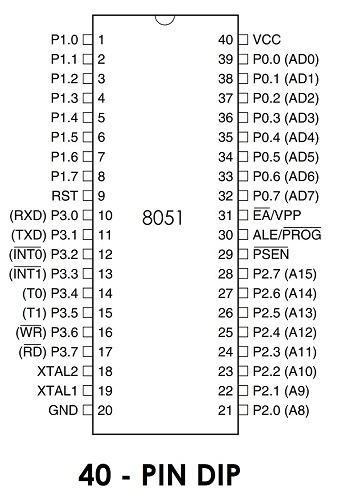
\includegraphics{/home/milav/Codes/MPMC/assets/imgs/181001_MCU_Question_Bank_Solved_html_f9cfed602ece3d54.png}
\caption{}
\end{figure}

\textbf{Pins 10 -- 17 (PORT 3):} Pins 10 to 17 form the PORT 3 pins of
the 8051 Microcontroller. PORT 3 also acts as a bidirectional Input /
Output PORT with internal pull-ups. Additionally, all the PORT 3 Pins
have special functions. The following table gives the details of the
additional functions of PORT 3 Pins.

\begin{longtable}[]{@{}lll@{}}
\toprule
PORT 3 Pin & Function & Description \\
\midrule
\endhead
P3.0 & RXD & Serial Input \\
P3.1 & TXD & Serial Output \\
P3.2 & INT0 & External Interrupt 0 \\
P3.3 & INT1 & External Interrupt 1 \\
P3.4 & T0 & Timer 0 \\
P3.5 & T1 & Timer 1 \\
P3.6 & WR & External Memory Write \\
P3.7 & RD & External Memory Read \\
\bottomrule
\end{longtable}

\textbf{Pins 18 \& 19:} Pins 18 and 19 i.e. XTAL 2 and XTAL 1 are the
pins for connecting external oscillator. Generally, a Quartz Crystal
Oscillator is connected here.

\textbf{Pin 20 (GND):} Pin 20 is the Ground Pin of the 8051
Microcontroller. It represents 0V and is connected to the negative
terminal (0V) of the Power Supply.

\textbf{Pins 21 -- 28 (PORT 2):} These are the PORT 2 Pins of the 8051
Microcontroller. PORT 2 is also a Bidirectional Port i.e. all the PORT 2
pins act as Input or Output. Additionally, when external memory is
interfaced, PORT 2 pins act as the higher order address byte. PORT 2
Pins have internal pull-ups.

\textbf{Pin 29 (PSEN):} Pin 29 is the Program Store Enable Pin (PSEN).
Using this pins, external Program Memory can be read.

\textbf{Pin 30 (ALE/PROG):} Pin 30 is the Address Latch Enable Pin.
Using this Pins, external address can be separated from data (as they
are multiplexed by 8051). During Flash Programming, this pin acts as
program pulse input (PROG).

\textbf{Pin 31 (EA/VPP):} Pin 31 is the External Access Enable Pin i.e.
allows external Program Memory. Code from external program memory can be
fetched only if this pin is LOW. For normal operations, this pins is
pulled HIGH. During Flash Programming, this Pin receives 12V Programming
Enable Voltage (VPP).

\textbf{Pins 32 -- 39 (PORT 0):} Pins 32 to 39 are PORT 0 Pins. They are
also bidirectional Input / Output Pins but without any internal
pull-ups. Hence, we need external pull-ups in order to use PORT 0 pins
as I/O PORT. In addition to acting as I/O PORT, PORT 0 also acts as
lower order address/data bus when external memory is accessed.

\textbf{Pin 40 (VCC):} Pin 40 is the power supply pin to which the
supply voltage is given (+5V).

\hypertarget{33-8051-microcontroller-block-diagram}{%
\subsection{3.3. 8051 Microcontroller Block
Diagram}\label{33-8051-microcontroller-block-diagram}}

\begin{figure}
\centering
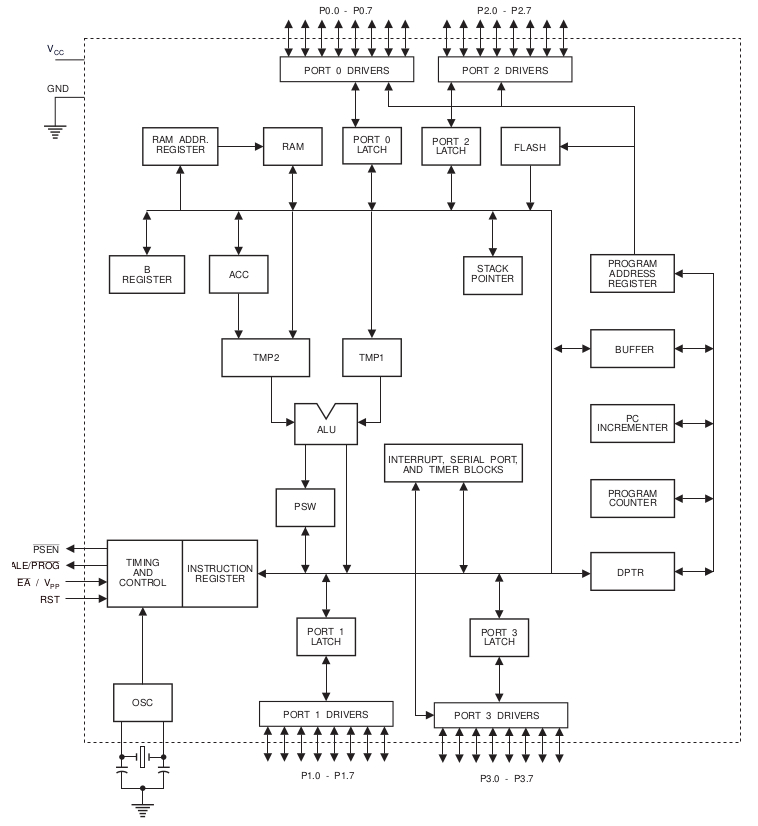
\includegraphics{/home/milav/Codes/MPMC/assets/imgs/181001_MCU_Question_Bank_Solved_html_9273ed43a6a941f5.jpg}
\caption{}
\end{figure}

\textbf{Central Processing Unit (CPU)}

\begin{itemize}
\item
  \textbf{ALU (Arithmetic Logic Unit):} The heart of calculations and
  logic operations. Performs arithmetic (addition, subtraction, etc.),
  logical (AND, OR, NOT) comparisons, and data manipulation.
\item
  \textbf{Instruction Decoder:} Decodes the instruction and generates
  control signals for other parts of the CPU.
\item
  \textbf{Timing and Control Unit:} Manages the fetch-decode-execute
  cycle of the CPU and synchronizes actions with other blocks.
\end{itemize}

\textbf{Registers}

\begin{itemize}
\item
  \textbf{Accumulator (A):} An 8-bit register used for most arithmetic
  and logical operations.
\item
  \textbf{B Register:} An 8-bit temporary register used for
  multiplication, division, and other data manipulation.
\item
  \textbf{Program Status Word (PSW):} Holds status flags like carry,
  overflow, parity, and register bank selection.
\item
  \textbf{Stack Pointer (SP):} Points to the top of the stack in RAM,
  used for subroutine calls and data storage.
\item
  \textbf{Program Counter (PC):} Keeps track of the memory address of
  the next instruction to be fetched.
\item
  \textbf{DPTR:} This is 16 bit register made up of two 8 bit registers
  -- DPH \& DPL. This register is used to point to Internal or External
  memory location.
\item
  \textbf{SFR:} Special Function Registers (SFRs) are special registers
  that contains control and status bits for Timer/Counter (TCON, TMOD),
  Interrupts (IE, IP), Serial Communication (SCON) and Power Control
  (PCON).
\item
  \textbf{Instruction Register:} Holds the currently fetched
  instruction.
\end{itemize}

\begin{figure}
\centering
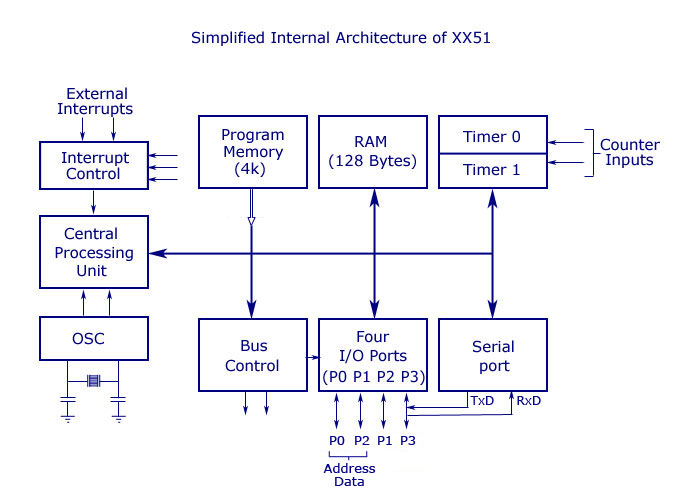
\includegraphics{/home/milav/Codes/MPMC/assets/imgs/181001_MCU_Question_Bank_Solved_html_a9f6d83e89bf83f5.jpg}
\caption{}
\end{figure}

\textbf{Memory}

\begin{itemize}
\item
  \textbf{Internal RAM (128 bytes):} Stores temporary data and variables
  during program execution.

  \begin{itemize}
  \item
    \textbf{Register Banks 0-3:} Four sets of eight 8-bit
    general-purpose registers.
  \item
    \textbf{Bit-addressable area (20h-2Fh):} 16 bytes with individually
    addressable bits.
  \item
    \textbf{General-purpose area (30h-7Fh):} Remaining 80 bytes for data
    and variables.
  \end{itemize}
\item
  \textbf{Internal ROM (typically 4KB):} Stores the program code of the
  microcontroller.
\end{itemize}

\textbf{Input/Output (I/O)}

\begin{itemize}
\item
  \textbf{Ports 0-3 (P0-P3):} Four 8-bit I/O ports that can be
  individually configured as input or output pins.
\end{itemize}

\textbf{Timers/Counters}

\begin{itemize}
\item
  \textbf{Timers/Counters 0 and 1 (T0, T1):} 16-bit timers/counters that
  can be used for various purposes like measuring time intervals,
  counting external events, and generating waveforms.
\end{itemize}

\textbf{Serial Port (UART)}

\begin{itemize}
\item
  \textbf{TXD (Transmit Data):} Transmits serial data out of the
  microcontroller.
\item
  \textbf{RXD (Receive Data):} Receives serial data into the
  microcontroller.
\item
  \textbf{SBUF (Serial Buffer):} Temporarily stores data during serial
  transmission or reception.
\end{itemize}

\textbf{Interrupts}

\begin{itemize}
\item
  \textbf{External Interrupts (INT0, INT1):} Triggered by signals on
  external pins.
\item
  \textbf{Timer Interrupts (TF0, TF1):} Triggered when timers overflow
  or reach a specific value.
\item
  \textbf{Serial Interrupts (RI, TI):} Triggered by events related to
  serial communication.
\item
  \textbf{Interrupt Control Logic:} Manages the enabling/disabling,
  prioritizing, and handling of interrupts.
\end{itemize}

\textbf{Additional Notes}

\begin{itemize}
\item
  \textbf{Bus Structure:} The 8051 uses an internal data bus to connect
  the CPU, memory, and I/O blocks. Instructions and data flow along this
  bus under the control of the CPU.
\item
  \textbf{Reset:} The RESET input initializes the 8051, setting
  registers and the Program Counter to their starting states.
\item
  \textbf{Oscillator:} The XTAL1 and XTAL2 inputs connect to the crystal
  and other components that generate the clock signal for the
  microcontroller.
\end{itemize}

\hypertarget{331-alu-arithmetic-logic-unit--timing-and-control-unit}{%
\subsubsection{3.3.1. ALU (Arithmetic Logic Unit) \& Timing and Control
Unit}\label{331-alu-arithmetic-logic-unit--timing-and-control-unit}}

\textbf{8051 ALU (Arithmetic Logic Unit)}

\begin{itemize}
\item
  \textbf{The Computational Heart:} The ALU is responsible for executing
  the core calculations and logical manipulations within the 8051
  microcontroller. As its name suggests, it handles two primary types of
  operations:
\item
  \textbf{Arithmetic Operations}

  \begin{itemize}
  \item
    Addition (\texttt{ADD})
  \item
    Subtraction (\texttt{SUBB})
  \item
    Multiplication (\texttt{MUL})
  \item
    Division (\texttt{DIV})
  \item
    Incrementing (\texttt{INC})
  \item
    Decrementing (\texttt{DEC})
  \end{itemize}
\item
  \textbf{Logical Operations}

  \begin{itemize}
  \item
    AND (\texttt{ANL})
  \item
    OR (\texttt{ORL})
  \item
    Exclusive-OR (\texttt{XRL})
  \item
    NOT (\texttt{CLR}, \texttt{CPL})
  \item
    Comparisons (for setting flags in the PSW register)
  \end{itemize}
\item
  \textbf{Key Components:}

  \begin{itemize}
  \item
    \textbf{Accumulator:} Data typically flows in and out of the
    Accumulator (A Register) during ALU operations.
  \item
    \textbf{Temporary Register:} Holds the second operand during
    calculations.
  \item
    \textbf{Arithmetic/Logic Circuits:} The actual hardware circuitry
    that performs the computations and manipulations.
  \end{itemize}
\item
  \textbf{Relationship to PSW:} The ALU interacts closely with the PSW
  register. ALU operations set flags like Carry (CY), Auxiliary Carry
  (AC), Overflow (OV), and Parity (P) in the PSW, which then become
  decision points for control flow in the program.
\end{itemize}

\textbf{8051 Timing and Control Unit}

\begin{itemize}
\item
  \textbf{Conductor of the Orchestra:} The Timing and Control Unit is
  the mastermind that synchronizes all the actions within the 8051
  microcontroller. It ensures everything happens at the right time and
  in the correct sequence.
\item
  \textbf{Key Functions:}

  \begin{itemize}
  \item
    \textbf{Instruction Fetching and Decoding:} Fetches instructions
    from memory and interprets their meaning, figuring out what actions
    need to be performed.
  \item
    \textbf{Machine Cycle and State Control:} Divides instructions into
    smaller steps (machine cycles) and generates timing signals that
    tell each part of the microcontroller when to do what.
  \item
    \textbf{Signal Generation:} Produces the precise electrical pulses
    that activate registers, the ALU, data buses, and other components
    within the microcontroller.
  \item
    \textbf{Interrupt Handling:} Coordinates what happens when an
    external event (like a timer overflow or a button press) interrupts
    the currently executing program.
  \end{itemize}
\item
  \textbf{Crystal Oscillator's Role:} The Timing and Control Unit relies
  on a crystal oscillator, generating a steady clock signal. This clock
  signal determines the fundamental speed at which the microcontroller
  operates.
\end{itemize}

\hypertarget{332-instruction-register-and-instruction-decoder}{%
\subsubsection{3.3.2. Instruction Register and Instruction
Decoder}\label{332-instruction-register-and-instruction-decoder}}

\textbf{Instruction Register (IR)}

\begin{itemize}
\item
  \textbf{Temporary Holding Area:} The Instruction Register is a
  special, temporary holding space within the microcontroller where the
  currently fetched instruction resides. It's closely connected to the
  Instruction Decoder.
\item
  \textbf{Size:} The size of the Instruction Register typically matches
  the width of instructions for the microcontroller. In the case of the
  8051, instructions can be 1, 2, or 3 bytes long, so the Instruction
  Register has to accommodate that.
\item
  \textbf{Two Main Parts (often):} In some architectures, the
  Instruction Register is divided into:

  \begin{itemize}
  \item
    \textbf{Shift Register:} Shifts in the instruction, bit by bit, as
    it's retrieved from memory. This process is synchronized with the
    microcontroller's clock.
  \item
    \textbf{Hold Register:} Holds the fully fetched instruction once the
    shifting is complete, making it available to the Instruction
    Decoder.
  \end{itemize}
\end{itemize}

\textbf{Instruction Decoder}

\begin{itemize}
\item
  \textbf{The Translator:} The Instruction Decoder is the circuit that
  analyzes the instruction currently residing in the Instruction
  Register. It breaks the instruction down into its meaningful
  components:
\item
  \textbf{Opcode:} The opcode (operation code) is the part of the
  instruction that tells the microcontroller what fundamental operation
  to perform (ADD, MOV, JUMP, etc.).
\item
  \textbf{Operands:} Operands are the pieces of data the instruction
  acts upon. This could be register names, immediate data (values
  hard-coded into the instruction), or memory addresses.
\item
  \textbf{Decoding Process:} The Instruction Decoder possesses
  'knowledge' of all valid instructions in the microcontroller's
  instruction set. It compares the opcode to this knowledge base to
  determine:

  \begin{itemize}
  \item
    What the operation is
  \item
    What type of operands are involved
  \item
    How many machine cycles are likely needed for execution
  \end{itemize}
\item
  \textbf{Control Signal Generation:} The Instruction Decoder produces
  control signals that activate different parts of the microcontroller,
  ensuring the correct actions are taken for the specified instruction.
  These signals will direct things like:

  \begin{itemize}
  \item
    Data transfers from registers to the ALU
  \item
    ALU operation selection (add, subtract, etc.)
  \item
    Setting of flags in the PSW register
  \item
    Flow of data to and from memory
  \end{itemize}
\end{itemize}

\textbf{The Dance of Fetching, Decoding, and Execution}

\begin{enumerate}
\def\labelenumi{\arabic{enumi}.}
\item
  \textbf{Fetch:} An instruction is retrieved from program memory, often
  with the help of the Program Counter.
\item
  \textbf{Load:} The instruction is shifted into the Instruction
  Register.
\item
  \textbf{Decode:} The Instruction Decoder analyzes the instruction and
  generates the appropriate control signals.
\item
  \textbf{Execute:} The microcontroller, directed by the control
  signals, carries out the steps required by the instruction.
\end{enumerate}

\hypertarget{333-accumulator-a}{%
\subsubsection{3.3.3. Accumulator (A)}\label{333-accumulator-a}}

\begin{itemize}
\item
  \textbf{The Workhorse:} The Accumulator is the central hub for most
  arithmetic, logical, and data transfer operations within the
  microcontroller. If you think of the microcontroller as a tiny
  calculator, the Accumulator is where you see the numbers being entered
  and the results being displayed.
\item
  \textbf{Key Operations:}

  \begin{itemize}
  \item
    \textbf{Arithmetic:} Addition, subtraction, incrementing,
    decrementing.
  \item
    \textbf{Logical:} AND, OR, XOR, NOT (complements), bit rotations,
    shifts.
  \item
    \textbf{Data Movement:} Transfers data to and from internal RAM or
    external memory.
  \end{itemize}
\item
  \textbf{Special Role in Instructions:} Many instructions in the
  microcontroller's instruction set implicitly use the Accumulator as
  either the source of data, the destination for the result, or both.
\end{itemize}

\hypertarget{334-register-b}{%
\subsubsection{3.3.4. Register B}\label{334-register-b}}

\begin{itemize}
\item
  \textbf{Versatile Assistant:} The B Register serves as a secondary
  register, often used to temporarily hold values to assist in
  calculations or data manipulation.
\item
  \textbf{Specialized Tasks:}

  \begin{itemize}
  \item
    \textbf{Multiplication and Division:} The B Register is essential
    for the \texttt{MUL\ AB} (multiply) and \texttt{DIV\ AB} (divide)
    instructions. It holds one of the operands and, in the case of
    division, stores the remainder of the operation.
  \item
    \textbf{Data Manipulation:} It can be used as a temporary holding
    space for values during complex operations that might involve
    multiple steps.
  \end{itemize}
\end{itemize}

\textbf{Key Points}

\begin{itemize}
\item
  \textbf{Size:} Both the Accumulator and B Register are usually 8-bit
  registers. This means they can each store a single byte of data (a
  value from 0 to 255).
\item
  \textbf{Not General Purpose:} Unlike general-purpose registers (like
  R0, R1, etc. in the 8051), the Accumulator and B Register have more
  defined roles due to their connection to specific instructions.
\end{itemize}

\hypertarget{335-pc-program-counter}{%
\subsubsection{3.3.5. PC (Program
Counter)}\label{335-pc-program-counter}}

\begin{itemize}
\item
  \textbf{The Program's Navigator:} The Program Counter holds the
  address of the next instruction to be executed by the microcontroller.
  It's like the microcontroller's bookmark within the program.
\item
  \textbf{How it Works:}

  \begin{enumerate}
  \def\labelenumi{\arabic{enumi}.}
  \item
    \textbf{Fetch:} The PC sends its current address to fetch the next
    instruction from program memory.
  \item
    \textbf{Increment:} By default, the PC is automatically incremented
    after fetching, preparing it for the following instruction.
  \item
    \textbf{Control Flow Changes:} Instructions like jumps
    (\texttt{JMP}) and calls (\texttt{CALL}) can change the PC's value,
    altering the program's execution order.
  \end{enumerate}
\item
  \textbf{Size:} The PC is 16 bits wide in the 8051, allowing it to
  address up to 64KB of program memory.
\end{itemize}

\hypertarget{336-sp-stack-pointer}{%
\subsubsection{3.3.6. SP (Stack Pointer)}\label{336-sp-stack-pointer}}

\begin{itemize}
\item
  \textbf{LIFO Storage:} The Stack Pointer points to the current 'top'
  of the stack. The stack is a last-in, first-out (LIFO) data structure
  within the 8051's internal RAM.
\item
  \textbf{Key Operations:}

  \begin{itemize}
  \item
    \textbf{PUSH:} Adds data to the top of the stack. The SP is then
    decremented to point to the new top.
  \item
    \textbf{POP:} Removes data from the top of the stack. The SP is
    incremented as data is removed.
  \end{itemize}
\item
  \textbf{Essential for:}

  \begin{itemize}
  \item
    \textbf{Subroutines (CALL and RET):} Stores the return address when
    a subroutine is called so the program knows where to resume after
    the subroutine finishes.
  \item
    \textbf{Interrupt Handling:} Stores register values when an
    interrupt occurs, preserving the state before the interrupt routine
    is executed.
  \end{itemize}
\item
  \textbf{Size:} The SP is 8 bits wide in the 8051.
\end{itemize}

\hypertarget{337-dptr-data-pointer}{%
\subsubsection{3.3.7. DPTR (Data Pointer)}\label{337-dptr-data-pointer}}

\begin{itemize}
\item
  \textbf{Accessing External Data:} The DPTR is a special 16-bit
  register used for addressing external memory (data memory outside the
  8051's internal space).
\item
  \textbf{Key Functions:}

  \begin{itemize}
  \item
    \textbf{Indirect Addressing:} The value in DPTR acts as a pointer.
    Instructions like \texttt{MOVX} (move external data) use DPTR to
    specify the source or destination address in external memory.
  \item
    \textbf{Lookup Tables:} DPTR is useful for storing the starting
    address of tables or data structures located in external memory.
  \end{itemize}
\end{itemize}

\hypertarget{338-special-function-registers-sfrs}{%
\subsubsection{3.3.8. Special Function Registers
(SFRs)}\label{338-special-function-registers-sfrs}}

\textbf{What is an SFR?}

\begin{itemize}
\item
  \textbf{Special Function Registers (SFRs)} are unique memory locations
  within the 8051 microcontroller's architecture. Unlike general-purpose
  RAM, SFRs directly control and configure various hardware peripherals
  and functions of the microcontroller.
\item
  \textbf{Location:} They occupy the address space from 80H to FFH
  within the internal RAM.
\end{itemize}

\textbf{Important 8051 SFRs}

\begin{longtable}[]{@{}lll@{}}
\toprule
Address (hex) & Register Name & Description \\
\midrule
\endhead
80 & P0 & Port 0 (Input/Output) \\
90 & P1 & Port 1 (Input/Output) \\
A0 & P2 & Port 2 (Input/Output) \\
B0 & P3 & Port 3 (Input/Output) \\
81 & SP & Stack Pointer \\
82 & DPL & Data Pointer Low Byte \\
83 & DPH & Data Pointer High Byte \\
87 & PCON & Power Control Register \\
88 & TCON & Timer/Counter 0 Control Register \\
89 & TMOD & Timer/Counter 0/1 Mode Register \\
8A & TL0 & Timer/Counter 0 Low Byte \\
8B & TL1 & Timer/Counter 1 Low Byte \\
8C & TH0 & Timer/Counter 0 High Byte \\
8D & TH1 & Timer/Counter 1 High Byte \\
98 & SCON & Serial Control Register \\
99 & SBUF & Serial Data Buffer \\
A8 & IE & Interrupt Enable Register \\
B8 & IP & Interrupt Priority Register \\
D0 & PSW & Program Status Word (contains flags) \\
E0 & ACC & Accumulator \\
F0 & B & B Register (auxiliary) \\
\bottomrule
\end{longtable}

Here's a breakdown of the most common 8051 SFRs, along with their roles:

\textbf{1. Accumulator (A)}

\begin{itemize}
\item
  \textbf{Address:} E0H
\item
  \textbf{Function:} The heart of most arithmetic and logical operations
  in the 8051. It acts as a source or destination for data.
\end{itemize}

\textbf{2. Program Status Word (PSW)}

\begin{itemize}
\item
  \textbf{Address:} D0H
\item
  \textbf{Function:} Contains critical flags indicating the status of
  the microcontroller, including:

  \begin{itemize}
  \item
    CY (Carry Flag)
  \item
    AC (Auxiliary Carry Flag)
  \item
    F0 (User-definable flag)
  \item
    RS1, RS0 (Register Bank select bits)
  \item
    OV (Overflow Flag)
  \item
    P (Parity Flag)
  \end{itemize}
\end{itemize}

\textbf{3. B Register (B)}

\begin{itemize}
\item
  \textbf{Address:} F0H
\item
  \textbf{Function:} Often used in conjunction with the Accumulator:

  \begin{itemize}
  \item
    Multiplication and division operations
  \item
    Temporary storage of data
  \end{itemize}
\end{itemize}

\textbf{4. Timer Registers}

\begin{itemize}
\item
  \textbf{TH0, TL0 (Timer 0):} 98H, 99H
\item
  \textbf{TH1, TL1 (Timer 1):} 8AH, 8BH
\item
  \textbf{Function:} Generate time delays, count external events, and
  form the basis of baud rate generation for serial communication.
\end{itemize}

\textbf{5. Serial Port Registers}

\begin{itemize}
\item
  \textbf{SBUF:} 99H

  \begin{itemize}
  \item
    Holds the data to be transmitted (write) or received data (read)
    during serial communication.
  \end{itemize}
\item
  \textbf{SCON:} 98H

  \begin{itemize}
  \item
    Controls the mode of serial communication (framing, baud rate,
    etc.).
  \end{itemize}
\end{itemize}

\textbf{6. Interrupt Registers}

\begin{itemize}
\item
  \textbf{IE (Interrupt Enable):} A0H

  \begin{itemize}
  \item
    Enables or disables specific interrupts.
  \end{itemize}
\item
  \textbf{IP (Interrupt Priority):} B0H

  \begin{itemize}
  \item
    Determines the priority level of different interrupt sources.
  \end{itemize}
\end{itemize}

\textbf{7. Port Registers (P0, P1, P2, P3)}

\begin{itemize}
\item
  \textbf{P0:} 80H
\item
  \textbf{P1:} 90H
\item
  \textbf{P2:} A0H
\item
  \textbf{P3:} B0H
\item
  \textbf{Function:} Control input and output operations on the 8051's
  I/O pins.
\end{itemize}

\textbf{8. Power Control Register (PCON)}

\begin{itemize}
\item
  \textbf{Address:} 87H
\item
  \textbf{Function:} Manages power-saving modes of the 8051 (idle mode,
  power-down mode).
\end{itemize}

\textbf{Note:} The exact set of SFRs can vary slightly depending on the
specific 8051 microcontroller variant you are using.

\textbf{How SFRs Work}

You can interact with SFRs in your programs just like regular memory
locations, using assembly language instructions or C extensions (like
\texttt{sfr}, \texttt{sfr16}, and \texttt{sbit}). By manipulating the
values in SFRs, you effectively configure the operation of the 8051.

\hypertarget{339-psw-program-status-word-address-0d0h-bit-addressable}{%
\subsubsection{3.3.9. PSW: Program Status Word (Address: 0D0H, Bit
addressable)}\label{339-psw-program-status-word-address-0d0h-bit-addressable}}

\begin{longtable}[]{@{}llllllll@{}}
\toprule
PSW.7 & PSW.6 & PSW.5 & PSW.4 & PSW.3 & PSW.2 & PSW.1 & PSW.0 \\
\midrule
\endhead
CY & AC & F0 & RS1 & RS0 & OV & - & P \\
\bottomrule
\end{longtable}

The PSW register is a vital SFR (Special Function Register) in the
functioning of a microcontroller. It reflects the status of the
operation that is being carried out in the processor. The PSW register
is bit and byte addressable. The physical address of PSW starts from
D0H. The individual bits are then accessed using D1, D2 \ldots{} D7.

\begin{longtable}[]{@{}ll@{}}
\toprule
Bit & Description \\
\midrule
\endhead
CY & Carry - Is set if data is coming out of bit 7 of Acc during an
Arithmetic operation. \\
AC & Auxiliary carry - This bit is set if data is coming out from bit 3
to bit 4 of Acc during an Arithmetic operation. \\
F0 & Flag 0 - User defined flag \\
RS1, RS0 & Register Bank select bits \\
OV & Overflow - OV flag is set if there is a carry from bit 6 but not
from bit 7 of an Arithmetic operation. It's also set if there is a carry
from bit 7 (but not from bit 6) of Acc. \\
P & Parity - This bit will be set if ACC has odd number of 1's after an
operation. If not, bit will remain cleared. \\
\bottomrule
\end{longtable}

\textbf{Register Bank Selection:}

\begin{longtable}[]{@{}lll@{}}
\toprule
RS1 (PSW.4) & RS0(PSW.3) & Register Bank Selected \\
\midrule
\endhead
0 & 0 & RB0 \\
0 & 1 & RB1 \\
1 & 0 & RB2 \\
1 & 1 & RB3 \\
\bottomrule
\end{longtable}

\hypertarget{3310-clock--reset-circuit}{%
\subsubsection{3.3.10. Clock \& Reset
Circuit}\label{3310-clock--reset-circuit}}

\textbf{Clock Circuit}

\begin{itemize}
\item
  \textbf{Crystal Oscillator:} The foundation of the timing for the 8051
  is a crystal oscillator connected to the XTAL1 and XTAL2 pins of the
  microcontroller.

  \begin{itemize}
  \item
    The crystal, along with small capacitors (usually in the 20-30pF
    range), provides a stable and precise clock frequency.
  \item
    Common crystal frequencies for 8051 systems are 11.0592 MHz or 12
    MHz.
  \end{itemize}
\item
  \textbf{Internal Clock Generation:} The 8051 has an internal clock
  generator that takes the external crystal oscillator's signal and
  divides it down. This ensures that the microcontroller and its various
  components operate at the correct internal clock speed.
\end{itemize}

\textbf{Diagram}

\begin{figure}
\centering
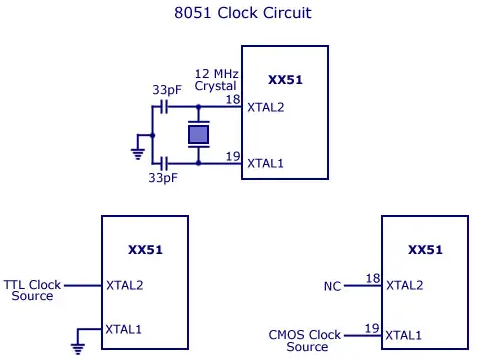
\includegraphics{https://www.circuitstoday.com/wp-content/uploads/2011/12/8051-Clock-Circuit.jpg}
\caption{}
\end{figure}

\textbf{Reset Circuit}

\begin{itemize}
\item
  \textbf{RC Network:} A simple resistor-capacitor (RC) network is often
  used for the reset circuit.

  \begin{itemize}
  \item
    When power is first applied, the capacitor begins to charge. This
    holds the RESET pin low for a short period, guaranteeing the 8051
    starts in a known state.
  \item
    Once the capacitor voltage reaches a threshold, the RESET pin goes
    high, allowing the microcontroller to begin executing code.
  \end{itemize}
\item
  \textbf{Supervisory Circuit (Optional):} For more robust reset
  control, a dedicated supervisory circuit/IC provides more precise
  monitoring of the power supply voltage. This ensures reliable resets
  if the power supply fluctuates or becomes unstable.
\end{itemize}

\textbf{Diagram}

\begin{figure}
\centering
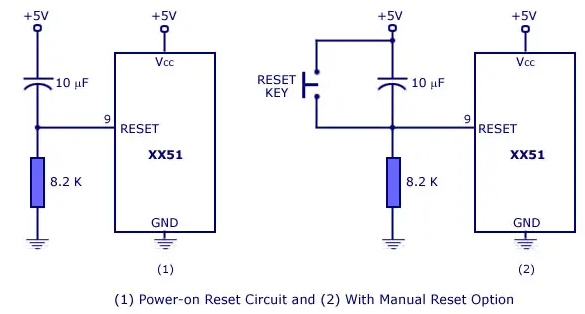
\includegraphics{https://www.circuitstoday.com/wp-content/uploads/2011/12/8051-reset-circuit.jpg}
\caption{}
\end{figure}

\textbf{Explanation}

\begin{enumerate}
\def\labelenumi{\arabic{enumi}.}
\item
  \textbf{Power On:} When the system powers on, the capacitor of the
  reset circuit is initially discharged, holding the RESET pin low.
\item
  \textbf{Reset:} This low level on the RESET pin forces the 8051
  microcontroller into a reset state. Internal registers are cleared,
  and the Program Counter begins at address 0000H.
\item
  \textbf{Capacitor Charging:} The capacitor in the reset circuit starts
  charging through the resistor.
\item
  \textbf{Reset Released:} Once the capacitor charges beyond the RESET
  pin's threshold voltage, the pin goes high. The 8051 starts executing
  code from the beginning of its program memory.
\item
  \textbf{Clock Stabilization:} While the reset circuit is active, the
  crystal oscillator begins to oscillate and the clock stabilizes. The
  8051's internal clock generator uses this signal to provide the
  necessary timing for the microcontroller's operation.
\end{enumerate}

\textbf{Key Points}

\begin{itemize}
\item
  The clock and reset circuits are essential for the correct
  initialization and operation of an 8051 microcontroller system.
\item
  Simple and inexpensive reset circuits can be designed using just a
  capacitor and resistor.
\item
  Supervisory circuits offer improved power monitoring and enhanced
  reset reliability.
\end{itemize}

\hypertarget{3311-io-ports}{%
\subsubsection{3.3.11. I/O Ports}\label{3311-io-ports}}

\textbf{General I/O Port Features}

\begin{itemize}
\item
  \textbf{Bidirectional:} All four I/O ports (Port 0, Port 1, Port 2,
  and Port 3) are bidirectional. Each pin can be configured as either an
  input or an output.
\item
  \textbf{Latches:} Each port has an associated latch that holds the
  output data. When a value is written to a port, it is stored in this
  latch, driving the output pins.
\item
  \textbf{Internal Pull-ups (Except Port 0):} Ports 1, 2, and 3 have
  built-in pull-up resistors. When configured as inputs, these resistors
  weakly pull the pins high. If you need a strong pull-down for a '0'
  input, you'll need to add external resistors.
\item
  \textbf{Dual Functionality:} Some port pins serve additional purposes,
  as explained below.
\end{itemize}

\textbf{Port 0 (P0)}

\begin{itemize}
\item
  \textbf{Address/Data Bus Duties:} Port 0 shares its pins to serve as:

  \begin{itemize}
  \item
    \textbf{The lower 8-bits of the address bus (AD0-AD7)} when
    connecting to external memory.
  \item
    \textbf{An 8-bit data bus (D0-D7)} for external memory read/write
    operations.
  \end{itemize}
\item
  \textbf{Open Drain:} Port 0's output drivers have an open-drain
  configuration. This means they can actively drive a pin low (logic
  '0'), but for high outputs (logic '1'), an external pull-up resistor
  is required.
\item
  \textbf{Needs Pull-Ups:} When used as general-purpose I/O, Port 0
  needs external pull-up resistors.
\end{itemize}

\textbf{Port 1 (P1)}

\begin{itemize}
\item
  \textbf{Standard I/O:} Primarily used as a general-purpose I/O port.
\item
  \textbf{No Additional Functions:} Pins of Port 1 don't have other
  roles like addressing.
\end{itemize}

\textbf{Port 2 (P2)}

\begin{itemize}
\item
  \textbf{Address Bus Duties:} When external memory is used, Port 2
  provides the upper 8-bits of the 16-bit address (A8-A15).
\item
  \textbf{Limited I/O Availability:} In systems with external memory,
  Port 2 loses its ability to be used for general-purpose input/output.
\end{itemize}

\textbf{Port 3 (P3)}

\begin{itemize}
\item
  \textbf{Diverse Roles:} Pins on Port 3 have multiple alternate
  functions, making it quite versatile:

  \begin{itemize}
  \item
    Serial Communication (RXD, TXD)
  \item
    Timer/Counter External Inputs
  \item
    Control Signals for External Memory (RD, WR)
  \item
    Interrupts
  \end{itemize}
\end{itemize}

\textbf{Important Notes:}

\begin{itemize}
\item
  \textbf{Initial State:} Upon reset, all I/O ports are configured as
  inputs.
\item
  \textbf{Configuring as Outputs:} To use a port pin as an output, you
  need to write a '1' to the corresponding bit in the port's SFR.
\item
  \textbf{Configuring as Inputs:} To use a port pin as an input, you
  must write a '1' to the corresponding bit in the port's SFR, ensuring
  the internal pull-ups are working as intended.
\end{itemize}

\textbf{Example (C code):}

\begin{Shaded}
\begin{Highlighting}[]
\PreprocessorTok{\#include }\ImportTok{\textless{}reg51.h\textgreater{}}\PreprocessorTok{ }\CommentTok{// Header file for 8051 SFRs}

\CommentTok{// Configure P1.0 as output, the rest of Port 1 as input}
\NormalTok{P1 }\OperatorTok{=} \BaseNTok{0x01}\OperatorTok{;}

\CommentTok{// Write a logic 1 (high) to P1.0}
\NormalTok{P1\_0 }\OperatorTok{=} \DecValTok{1}\OperatorTok{;}

\CommentTok{// Read the value from P1.5}
\DataTypeTok{unsigned} \DataTypeTok{char}\NormalTok{ input\_value }\OperatorTok{=}\NormalTok{ P1\_5}\OperatorTok{;}
\end{Highlighting}
\end{Shaded}

\hypertarget{33111-port-0-pin-structure}{%
\paragraph{3.3.11.1. Port-0 Pin
Structure}\label{33111-port-0-pin-structure}}

\begin{itemize}
\item
  \textbf{Dual Purpose:}

  \begin{itemize}
  \item
    \textbf{General Purpose I/O:} Can be configured as a standard 8-bit
    bidirectional input/output port.
  \item
    \textbf{Address/Data Bus:} Serves as the lower 8-bits of the address
    bus (AD0-AD7) and the data bus (D0-D7) when interfacing with
    external memory.
  \end{itemize}
\item
  \textbf{Open-Drain Outputs:} Port 0 pins use an open-drain
  configuration for outputs. This means they can actively drive a pin
  low (logic '0'), but require an external pull-up resistor to achieve a
  high output (logic '1').
\item
  \textbf{Latch:} Each Port 0 pin is connected to a latch. Data written
  to the P0 SFR (Special Function Register) is held in this latch.
\item
  \textbf{Internal Diagram (Simplified):}
\end{itemize}

\begin{figure}
\centering
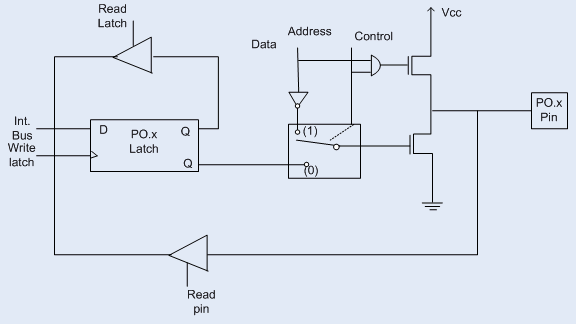
\includegraphics{/home/milav/Codes/MPMC/assets/imgs/181001_MCU_Question_Bank_Solved_html_3411f9b9256cfcd0.png}
\caption{}
\end{figure}

\textbf{Operation}

\begin{itemize}
\item
  \textbf{Input Mode:}

  \begin{enumerate}
  \def\labelenumi{\arabic{enumi}.}
  \item
    To configure as input, write a '1' to the corresponding latch bit.
  \item
    Both output MOSFETs are turned off, resulting in a high-impedance
    state.
  \item
    External devices or pull-up resistors determine the pin's voltage
    level.
  \end{enumerate}
\item
  \textbf{Output Mode:}

  \begin{enumerate}
  \def\labelenumi{\arabic{enumi}.}
  \item
    \textbf{Writing '0':} The lower MOSFET turns on, pulling the pin to
    ground (logic '0').
  \item
    \textbf{Writing '1':}

    \begin{itemize}
    \item
      Both MOSFETs turn off, resulting in a high-impedance state.
    \item
      An external pull-up resistor is \textbf{required} to achieve a
      high output (logic '1').
    \end{itemize}
  \end{enumerate}
\item
  \textbf{External Memory Interfacing:}

  \begin{enumerate}
  \def\labelenumi{\arabic{enumi}.}
  \item
    A control signal (likely ALE) determines if Port 0 functions in
    address/data mode.
  \item
    When acting as the address/data bus:

    \begin{itemize}
    \item
      \textbf{'0' Output:} Lower MOSFET on, upper MOSFET off.
    \item
      \textbf{'1' Output:} Lower MOSFET off, upper MOSFET on (the bus
      itself will pull the line high).
    \end{itemize}
  \end{enumerate}
\end{itemize}

\textbf{Key Points}

\begin{itemize}
\item
  \textbf{Pull-up Resistors:} Port 0 absolutely requires external
  pull-up resistors when used as general-purpose I/O in situations where
  you need to output a logic '1'.
\item
  \textbf{Versatility with Tradeoffs:} The dual-functionality of Port 0
  offers flexibility, but adds a layer of complexity when interfacing
  external memory.
\end{itemize}

\hypertarget{33112-port-1-pin-structure}{%
\paragraph{3.3.11.2. Port 1 Pin
Structure}\label{33112-port-1-pin-structure}}

\begin{itemize}
\item
  \textbf{Dedicated I/O:} Port 1 is a simple 8-bit bidirectional I/O
  port. Its pins do not have any additional alternate functionality like
  serving as address lines or special control signals.
\item
  \textbf{Internal Pull-up Resistors:} A crucial feature of Port 1 is
  that each pin is connected to a weak internal pull-up resistor. These
  resistors are automatically enabled when the port pin is configured as
  an input.
\item
  \textbf{Internal Diagram (Simplified):}
\end{itemize}

\begin{figure}
\centering
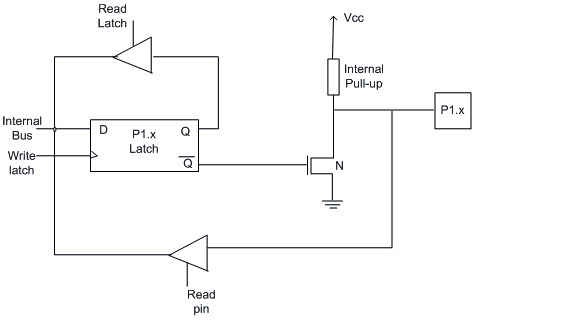
\includegraphics{/home/milav/Codes/MPMC/assets/imgs/181001_MCU_Question_Bank_Solved_html_1bbcd9539232851b.png}
\caption{}
\end{figure}

\textbf{Operation}

\begin{itemize}
\item
  \textbf{Input Mode:}

  \begin{enumerate}
  \def\labelenumi{\arabic{enumi}.}
  \item
    To configure as input, write a '1' to the corresponding latch bit.
  \item
    The internal pull-up resistor weakly pulls the pin towards a high
    voltage level (logic '1').
  \item
    To read a logic '0', an external device must be strong enough to
    overcome the internal pull-up and pull the pin to ground.
  \end{enumerate}
\item
  \textbf{Output Mode:}

  \begin{enumerate}
  \def\labelenumi{\arabic{enumi}.}
  \item
    To configure as output, write a '0' or '1' to the corresponding
    latch bit.
  \item
    The internal pull-up resistor is effectively overridden.
  \item
    \textbf{Writing '0':} The output driver actively pulls the pin low.
  \item
    \textbf{Writing '1':} The output becomes high-impedance, but the
    internal pull-up resistor weakly pulls the pin towards a high state.
  \end{enumerate}
\end{itemize}

\textbf{Important Considerations}

\begin{itemize}
\item
  \textbf{Weak Pull-ups:} The internal pull-up resistors on Port 1 are
  relatively weak. If a connected external device attempts to strongly
  drive a pin low, it might not be able to fully bring the voltage to a
  valid logic '0' level.
\item
  \textbf{Sinking Current:} When a Port 1 pin is configured as an input
  and an external device drives it low, the external circuitry needs to
  be able to sink the current flowing through the internal pull-up
  resistor.
\item
  \textbf{Potential for Incorrect Readings:} If an external device is
  not strong enough or is configured incorrectly, the input may not
  register a true '0' even when the external device intends to drive it
  low.
\end{itemize}

\textbf{Recommendations}

\begin{itemize}
\item
  \textbf{Input Considerations:} If using Port 1 for inputs where strong
  logic '0' signals are needed, consider either:

  \begin{itemize}
  \item
    Disabling the internal pull-ups (if software/hardware allows it) and
    using external pull-down resistors.
  \item
    Using a different port without built-in pull-ups.
  \end{itemize}
\item
  \textbf{Output Considerations:} Port 1 can drive outputs effectively,
  but keep in mind that writing a '1' relies on the internal pull-up or
  an external pull-up to achieve the high state.
\end{itemize}

\hypertarget{33113-port-2-pin-structure}{%
\paragraph{3.3.11.3. Port 2 Pin
Structure}\label{33113-port-2-pin-structure}}

\begin{itemize}
\item
  \textbf{Dual Roles:}

  \begin{enumerate}
  \def\labelenumi{\arabic{enumi}.}
  \item
    \textbf{Higher Order Address Bus:} When the 8051 is interfaced with
    external memory, Port 2 provides the upper 8-bits of the 16-bit
    address (A8-A15).
  \item
    \textbf{General Purpose I/O:} If external memory is not in use, Port
    2 can function as a standard 8-bit bidirectional I/O port.
  \end{enumerate}
\item
  \textbf{Internal Pull-up Resistors:} Similar to Port 1, each pin of
  Port 2 has an internal pull-up resistor that is active when the pin is
  configured as an input.
\item
  \textbf{Internal Diagram (Simplified):}
\end{itemize}

\begin{figure}
\centering
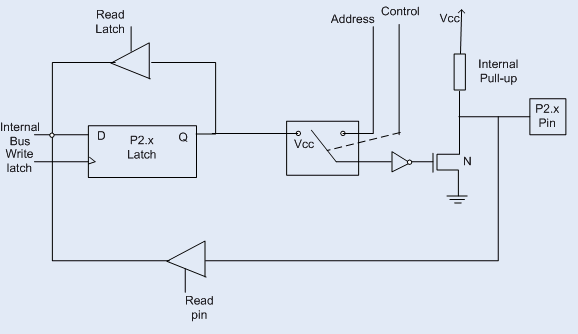
\includegraphics{/home/milav/Codes/MPMC/assets/imgs/181001_MCU_Question_Bank_Solved_html_ff86744d95f884c6.png}
\caption{}
\end{figure}

\textbf{Operation}

\begin{itemize}
\item
  \textbf{Input Mode:}

  \begin{enumerate}
  \def\labelenumi{\arabic{enumi}.}
  \item
    To configure as input, write a '1' to the corresponding latch bit.
  \item
    The internal pull-up weakly pulls the pin high (logic '1').
  \item
    External devices must be strong enough to overcome the pull-up
    resistor to drive a logic '0'.
  \end{enumerate}
\item
  \textbf{Output Mode:}

  \begin{enumerate}
  \def\labelenumi{\arabic{enumi}.}
  \item
    To configure as output, write a '0' or '1' to the corresponding
    latch bit.
  \item
    The output driver actively drives the pin high or low, overriding
    the internal pull-up.
  \end{enumerate}
\item
  \textbf{External Memory Interfacing:}

  \begin{enumerate}
  \def\labelenumi{\arabic{enumi}.}
  \item
    When used as the higher address byte, the Port 2 latch holds the
    address information.
  \item
    Latch values remain stable during external memory operations.
  \end{enumerate}
\end{itemize}

\textbf{Important Considerations}

\begin{itemize}
\item
  \textbf{Limited Current Capacity:} As with Port 1, the internal
  pull-ups on Port 2 mean it's not ideal for driving heavy loads or
  sinking significant current, especially in input mode.
\item
  \textbf{Conflict with External Memory:} When using external memory,
  Port 2's general-purpose I/O functionality is effectively unavailable.
\item
  \textbf{Design Trade-offs:} The dual-role capability of Port 2 adds
  flexibility, but requires careful consideration of its function in
  relation to other system requirements.
\end{itemize}

\textbf{Recommendations}

\begin{itemize}
\item
  \textbf{Input Considerations:} The same recommendations for Port 1
  apply to Port 2. Consider external pull-down resistors or disabling
  the internal pull-ups if reliable '0' inputs are crucial and your
  external devices are weak drivers.
\item
  \textbf{External Memory Considerations:} If using external memory,
  avoid relying on Port 2 for general-purpose inputs.
\end{itemize}

\hypertarget{33114-port-3-pin-structure}{%
\paragraph{3.3.11.4. Port 3 Pin
Structure}\label{33114-port-3-pin-structure}}

\begin{itemize}
\item
  \textbf{Multifunctional:} Port 3, unlike Ports 1 and 2, is the most
  versatile port on the 8051. Each of its 8 pins (P3.0-P3.7) can serve
  either as a general-purpose I/O pin or take on a specialized alternate
  function.
\item
  \textbf{Internal Pull-ups:} Each pin on Port 3 has a weak internal
  pull-up resistor, similar to Ports 1 and 2. This pull-up is active
  when the pin is configured as an input.
\item
  \textbf{Alternate Function Control:}

  \begin{itemize}
  \item
    \textbf{Latch:} Each Port 3 bit has a corresponding latch bit.
    Writing a '1' to the latch allows the alternate function to be used.
  \item
    \textbf{Priority:} If multiple alternate functions compete for the
    same pin, a priority system exists to determine which function takes
    precedence.
  \end{itemize}
\item
  \textbf{Internal Diagram (Simplified):}
\end{itemize}

\begin{figure}
\centering
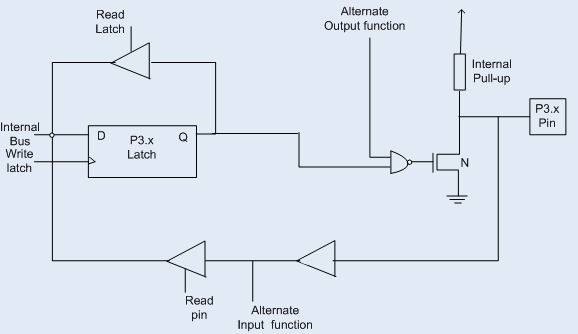
\includegraphics{/home/milav/Codes/MPMC/assets/imgs/181001_MCU_Question_Bank_Solved_html_1523265967e3e07f.png}
\caption{}
\end{figure}

\textbf{Alternate Functions of Port 3}

\begin{longtable}[]{@{}lll@{}}
\toprule
PORT 3 Pin & Function & Description \\
\midrule
\endhead
P3.0 & RXD & Serial Data Receive for UART communication. \\
P3.1 & TXD & Serial Data Transmit for UART communication. \\
P3.2 & INT0 & External Interrupt 0 input. \\
P3.3 & INT1 & External Interrupt 1 input. \\
P3.4 & T0 & Timer/Counter 0 external input. \\
P3.5 & T1 & Timer/Counter 1 external input. \\
P3.6 & WR & Write strobe for external memory. \\
P3.7 & RD & Read strobe for external memory. \\
\bottomrule
\end{longtable}

\textbf{Operation}

\begin{itemize}
\item
  \textbf{Input Mode:}

  \begin{enumerate}
  \def\labelenumi{\arabic{enumi}.}
  \item
    Write a '1' to the pin's latch bit.
  \item
    The internal pull-up pulls the pin high.
  \item
    External devices must overcome the pull-up to drive a strong logic
    '0'.
  \end{enumerate}
\item
  \textbf{Output Mode:}

  \begin{enumerate}
  \def\labelenumi{\arabic{enumi}.}
  \item
    Write a '0' or '1' to the pin's latch bit.
  \item
    Output drivers actively drive the pin high or low.
  \end{enumerate}
\item
  \textbf{Alternate Function Mode:}

  \begin{enumerate}
  \def\labelenumi{\arabic{enumi}.}
  \item
    Write a '1' to the corresponding latch bit to enable the alternate
    function.
  \item
    The pin is now dedicated to its special role (serial communication,
    interrupt, etc.).
  \end{enumerate}
\end{itemize}

\textbf{Important Notes}

\begin{itemize}
\item
  \textbf{Flexibility and Tradeoffs:} Port 3's versatility comes at the
  cost of reduced I/O capability if many alternate functions are in use.
\item
  \textbf{Configuration:} Careful software configuration is essential to
  determine whether a Port 3 pin acts as general-purpose I/O or in its
  alternate function role.
\end{itemize}

\hypertarget{34-memory-organization}{%
\subsection{3.4. Memory Organization}\label{34-memory-organization}}

\hypertarget{341-program-memory-rom}{%
\subsubsection{3.4.1. Program Memory
(ROM)}\label{341-program-memory-rom}}

\begin{itemize}
\item
  \textbf{Purpose:} The program memory is where the 8051 stores the
  instructions that make up the program it's executing. Think of it as
  the microcontroller's 'recipe book' of code.
\item
  \textbf{Types:}

  \begin{itemize}
  \item
    \textbf{Internal ROM:} Most 8051 derivatives have some amount of
    built-in program memory (often around 4KB).
  \item
    \textbf{External ROM:} If a program is too large to fit in the
    internal ROM, the 8051 can interface with external memory chips to
    expand its program storage.
  \end{itemize}
\item
  \textbf{Non-volatile:} This means that the program code remains stored
  even when the 8051 loses power.
\item
  \textbf{Access Control:} The external memory is accessed through the
  External Access (EA) pin. By default, the EA pin is connected to VCC,
  so the microcontroller fetches instructions from internal memory
  first. If the program size exceeds 4KB, the microcontroller will
  automatically switch to external memory. To force the microcontroller
  to use external memory only, connect the EA pin to GND.
\end{itemize}

\textbf{Diagram (Program Memory)}

\begin{figure}
\centering
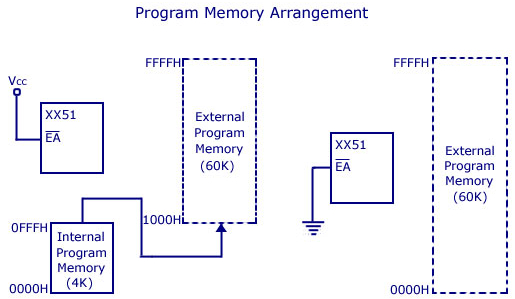
\includegraphics{/home/milav/Codes/MPMC/assets/imgs/181001_MCU_Question_Bank_Solved_html_9e16af640b46000c.jpg}
\caption{}
\end{figure}

A simplified visual representation of program memory might look like
this:

\begin{Shaded}
\begin{Highlighting}[]
\NormalTok{+{-}{-}{-}{-}{-}{-}{-}{-}{-}{-}{-}{-}{-}{-}{-}{-}{-}{-}{-}{-}+}
\NormalTok{| Program Memory (ROM)|}
\NormalTok{+{-}{-}{-}{-}{-}{-}{-}{-}{-}{-}{-}{-}{-}{-}{-}{-}{-}{-}{-}{-}+}
\NormalTok{|  Instruction 1      |}
\NormalTok{|  Instruction 2      |}
\NormalTok{|        ...          |}
\NormalTok{|  Instruction N      |}
\NormalTok{+{-}{-}{-}{-}{-}{-}{-}{-}{-}{-}{-}{-}{-}{-}{-}{-}{-}{-}{-}{-}+}
\end{Highlighting}
\end{Shaded}

\hypertarget{342-data-memory-ram}{%
\subsubsection{3.4.2. Data Memory (RAM)}\label{342-data-memory-ram}}

\begin{itemize}
\item
  \textbf{Purpose:} The data memory acts as the 8051's workspace. It
  holds temporary variables, intermediate calculations, and other data
  the program needs while running.
\item
  \textbf{Types}

  \begin{itemize}
  \item
    \textbf{Internal RAM:} The 8051 has a limited amount of internal RAM
    (usually 128 bytes).
  \item
    \textbf{External RAM:} Like with program memory, the 8051 can
    utilize external RAM for additional data storage.
  \end{itemize}
\item
  \textbf{Volatile:} Data in RAM is lost when the 8051 loses power.
\end{itemize}

\textbf{Structure of Internal Data Memory}

\begin{figure}
\centering
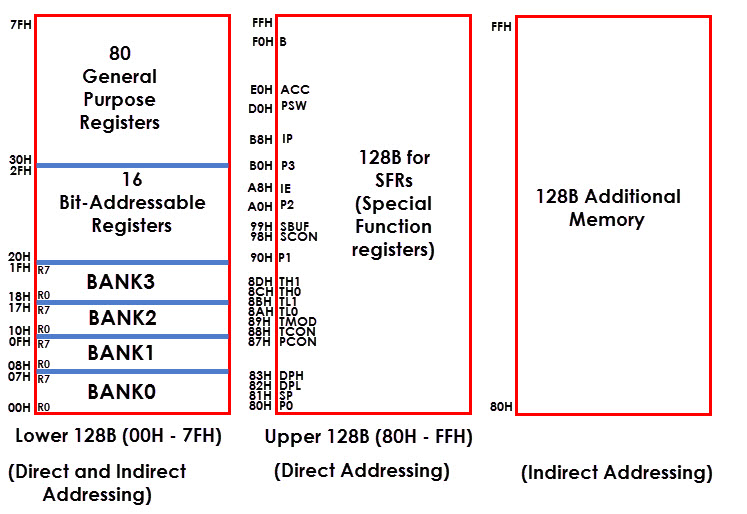
\includegraphics{/home/milav/Codes/MPMC/assets/imgs/181001_MCU_Question_Bank_Solved_html_c061f3a98a4f76b6.png}
\caption{}
\end{figure}

Most modern 8051 variants provide 256 bytes of internal RAM, which is
organized into the following distinct areas:

\textbf{1. Working Registers (00H - 1FH)}

\begin{itemize}
\item
  \textbf{Register Banks:} The first 32 bytes of RAM are divided into
  four register banks (Bank 0, Bank 1, Bank 2, Bank 3). Each bank
  contains eight general-purpose registers (R0-R7).
\item
  \textbf{Addressing:}

  \begin{itemize}
  \item
    \textbf{By Name:} Access registers by name (R0, R1, etc.) after
    selecting the appropriate bank using the RS0 and RS1 bits in the
    Program Status Word (PSW) register.
  \item
    \textbf{By Address} Access registers directly by their address
    (e.g., 12H for R2 in Bank 2), regardless of the currently selected
    bank.
  \end{itemize}
\end{itemize}

\textbf{2. Bit-Addressable Memory (20H - 2FH)}

\begin{itemize}
\item
  \textbf{Individual Bit Control:} This area contains 128 individually
  addressable bits (00H - 7FH within the byte range 20H-2FH). This is
  efficient for storing single-bit values like flags or control signals.
\end{itemize}

\textbf{3. General Purpose RAM (Scratchpad) (30H - 7FH)}

\begin{itemize}
\item
  \textbf{Flexible Storage:} This 80-byte area provides general-purpose
  data storage for variables and temporary data.
\item
  \textbf{Stack:} The stack, used for storing function call return
  addresses and temporary storage during interrupts, also resides within
  this area.
\end{itemize}

\textbf{4. Special Function Registers (SFRs) (80H - FFH)}

\begin{longtable}[]{@{}lll@{}}
\toprule
Address (hex) & Register Name & Description \\
\midrule
\endhead
80 & P0 & Port 0 (Input/Output) \\
90 & P1 & Port 1 (Input/Output) \\
A0 & P2 & Port 2 (Input/Output) \\
B0 & P3 & Port 3 (Input/Output) \\
81 & SP & Stack Pointer \\
82 & DPL & Data Pointer Low Byte \\
83 & DPH & Data Pointer High Byte \\
87 & PCON & Power Control Register \\
88 & TCON & Timer/Counter 0 Control Register \\
89 & TMOD & Timer/Counter 0/1 Mode Register \\
8A & TL0 & Timer/Counter 0 Low Byte \\
8B & TL1 & Timer/Counter 1 Low Byte \\
8C & TH0 & Timer/Counter 0 High Byte \\
8D & TH1 & Timer/Counter 1 High Byte \\
98 & SCON & Serial Control Register \\
99 & SBUF & Serial Data Buffer \\
A8 & IE & Interrupt Enable Register \\
B8 & IP & Interrupt Priority Register \\
D0 & PSW & Program Status Word (contains flags) \\
E0 & ACC & Accumulator \\
F0 & B & B Register (auxiliary) \\
\bottomrule
\end{longtable}

\begin{itemize}
\item
  \textbf{Hardware Control:} SFRs occupy the upper 128 bytes of RAM and
  directly control various hardware functions of the 8051, such as:

  \begin{itemize}
  \item
    I/O Ports (P0, P1, P2, P3)
  \item
    Program Status Word (PSW)
  \item
    Accumulator (A)
  \item
    Interrupt Control (IE, IP)
  \item
    Power Management (PCON)
  \end{itemize}
\item
  \textbf{Direct Addressing Only:} SFRs can only be accessed using their
  specific addresses. Unused addresses within this range are reserved
  and cannot be used for general-purpose data storage.
\end{itemize}

\textbf{Key Points}

\begin{itemize}
\item
  \textbf{Indirect Addressing:} The lower 128 bytes of RAM (working
  registers, bit-addressable area, and scratchpad) can be addressed both
  directly (by their address) and indirectly (using a register to hold
  the address).
\item
  \textbf{Limited RAM Capacity:} The 8051's internal RAM is relatively
  small. Many applications require interfacing external RAM to support
  larger datasets.
\item
  \textbf{Variant Differences:} Some 8051 variants may have an
  additional 128 bytes of RAM sharing the same address space as SFRs.
  This extra RAM is usually only accessible via indirect addressing.
\item
  \textbf{Speed:} Internal RAM is extremely fast to access compared to
  external RAM, as it's located directly on the microcontroller chip.
\item
  \textbf{Flexibility:} The bit-addressable area provides fine-grained
  control over individual bits, ideal for control and status flags.
\end{itemize}

\textbf{How Internal RAM Is Used}

\begin{itemize}
\item
  \textbf{Arithmetic and Logical Operations}: The register banks are
  heavily used by the ALU for arithmetic and logical operations.
\item
  \textbf{Temporary Storage:} All sections of the internal RAM can be
  used for temporarily storing data during calculation or program
  execution.
\item
  \textbf{Stack:} Although the 8051 has a dedicated hardware stack, the
  general-purpose RAM can also be used as a stack area in constrained
  situations.
\item
  \textbf{Flags and Control:} The bit-addressable area often houses
  individual control flags and status bits for the 8051 or its
  peripherals.
\end{itemize}

\textbf{Example}

\begin{Shaded}
\begin{Highlighting}[]
\NormalTok{MOV R1, \#50H  ; Move the value 50H into register R1}
\NormalTok{ADD A, R1     ; Add the value in R1 to the accumulator}
\NormalTok{MOV 35H, A    ; Store the result in general{-}purpose RAM location 35H}
\NormalTok{SETB PSW.2    ; Set bit 2 (Carry flag) in the Program Status Word}
\end{Highlighting}
\end{Shaded}

\hypertarget{343-external-memory-interfacing-and-decoding-logic}{%
\subsubsection{3.4.3. External Memory Interfacing and Decoding
Logic}\label{343-external-memory-interfacing-and-decoding-logic}}

\textbf{External Memory Interfacing in the 8051}

The 8051 microcontroller offers limited internal program and data
memory, which might not be sufficient for complex applications. To
expand its memory capacity, the 8051 can be interfaced with external
memory devices like ROM and RAM. This capability allows you to store
larger programs and work with more data.

\textbf{Key Components Involved:}

\begin{itemize}
\item
  \textbf{Microcontroller:} The 8051 itself, responsible for controlling
  data flow and program execution.
\item
  \textbf{External Memory:} ROM chips for program storage and RAM chips
  for data storage. Both can be up to 64KB in size.
\item
  \textbf{Address Decoding Logic:} Circuitry that translates the
  microcontroller's memory addresses into specific chip select signals
  for each external memory device.
\item
  \textbf{Control Signals:} Signals like PSEN (Program Store Enable), RD
  (Read), and WR (Write) from the microcontroller to control external
  memory operations.
\item
  \textbf{Data Bus:} A bidirectional bus that carries data between the
  microcontroller and external memory.
\end{itemize}

\textbf{Addressing and Decoding Process:}

\begin{enumerate}
\def\labelenumi{\arabic{enumi}.}
\item
  \textbf{Memory Access Initiation:} The microcontroller initiates a
  memory access operation, specifying an address and indicating whether
  it's a read or write operation.
\item
  \textbf{Address Bus Decoding:} The address decoding logic receives the
  address from the microcontroller.
\item
  \textbf{Chip Select Generation:} Based on the decoded address and the
  memory map, the decoding logic generates individual chip select
  signals for the appropriate ROM or RAM chip(s).
\item
  \textbf{Control Signal Assertion:} The microcontroller asserts control
  signals like PSEN, RD, or WR along with the data (for write
  operations) onto the control and data buses.
\item
  \textbf{Data Transfer:} The selected memory chip(s) perform the read
  or write operation based on the control signals and data provided.
\item
  \textbf{Data Bus Interaction:} The data is transferred between the
  microcontroller and the selected memory chip(s) on the data bus.
\end{enumerate}

\textbf{Example:}

Imagine the microcontroller wants to read data from byte address 40000
(64KB ROM, 0-31KB for ROM, 32KB-63KB for RAM) in external memory.

\begin{enumerate}
\def\labelenumi{\arabic{enumi}.}
\item
  The address 40000 is sent to the address decoding logic.
\item
  The logic recognizes it's within the ROM address range (0-31KB) and
  generates a chip select for the ROM chip.
\item
  The microcontroller asserts the RD (read) signal and places the
  address 40000 on the address bus.
\item
  The selected ROM chip reads the data at byte address 40000 and places
  it on the data bus.
\item
  The microcontroller reads the data from the data bus and stores it
  internally.
\end{enumerate}

The below image shows a simplified block diagram of interfacing 64KB ROM
and 64KB RAM with the 8051:

\begin{figure}
\centering
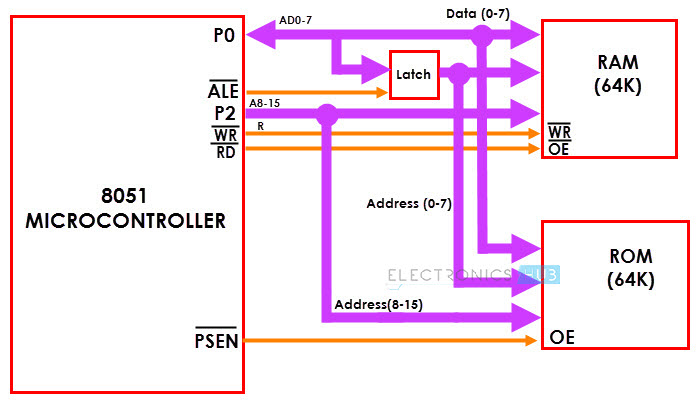
\includegraphics{/home/milav/Codes/MPMC/assets/imgs/181001_MCU_Question_Bank_Solved_html_80c7f2d8ec8c6f6f.png}
\caption{}
\end{figure}

\begin{itemize}
\item
  \textbf{Microcontroller:} Represented by the 8051 block.
\item
  \textbf{External Memory:} ROM and RAM blocks labeled as "64K ROM" and
  "64K RAM".
\item
  \textbf{Address Decoding Logic:} Not explicitly shown but implied by
  the connections between the address bus and chip select signals.
\item
  \textbf{Control Signals:} PSEN, RD, and WR signals are shown from the
  microcontroller.
\item
  \textbf{Data Bus:} Represented by the bidirectional "Data (0-7)"
  lines.
\end{itemize}

\hypertarget{35-stack-stack-pointer-and-stack-operations}{%
\subsection{3.5. Stack, Stack Pointer, and Stack
Operations}\label{35-stack-stack-pointer-and-stack-operations}}

\textbf{What is the Stack?}

\begin{itemize}
\item
  \textbf{LIFO Structure:} The stack is a section of the 8051's internal
  RAM that follows a Last-In, First-Out (LIFO) principle. Imagine it
  like a stack of plates; you always add and remove from the top.
\item
  \textbf{Purpose:}

  \begin{itemize}
  \item
    \textbf{Temporary Storage:} The stack stores data temporarily during
    program execution.
  \item
    \textbf{Function Calls:} It saves the return address when a function
    (subroutine) is called, allowing the program to return to the
    correct point after the function completes.
  \item
    \textbf{Interrupts:} When an interrupt occurs, the 8051 temporarily
    pushes the current program counter (PC) onto the stack, allowing it
    to later resume execution where it was interrupted.
  \end{itemize}
\end{itemize}

\textbf{Stack Pointer (SP)}

\begin{itemize}
\item
  \textbf{Address Tracker:} The Stack Pointer (SP) is an 8-bit register
  that holds the address of the top of the stack (the last item added).
\item
  \textbf{Initialization:} Upon reset, the SP is usually initialized to
  07H within the 8051's internal RAM.
\item
  \textbf{Dynamic:} The SP changes automatically during stack operations
  (push and pop).
\end{itemize}

\begin{figure}
\centering
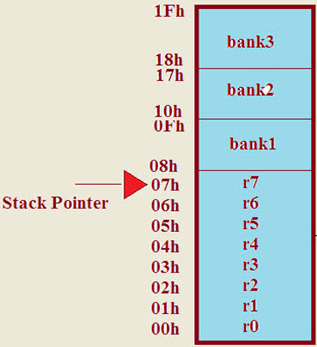
\includegraphics{/home/milav/Codes/MPMC/assets/imgs/181001_MCU_Question_Bank_Solved_html_d922510a8750c6be.jpg}
\caption{}
\end{figure}

\textbf{Stack Operations}

\begin{enumerate}
\def\labelenumi{\arabic{enumi}.}
\item
  \textbf{PUSH Instruction:}

  \begin{itemize}
  \item
    \textbf{Stores Data:} The PUSH instruction puts a byte of data onto
    the top of the stack.
  \item
    \textbf{SP Modification:}

    \begin{enumerate}
    \def\labelenumii{\arabic{enumii}.}
    \item
      The SP is incremented.
    \item
      The data is then stored at the memory location now pointed to by
      the SP.
    \end{enumerate}
  \end{itemize}
\end{enumerate}

\textbf{PUSH Example:}

\begin{Shaded}
\begin{Highlighting}[]
\NormalTok{MOV R6, \#25H}
\NormalTok{MOV R1, \#12H}
\NormalTok{MOV R4, \#0F3H}
\NormalTok{PUSH R6}
\NormalTok{PUSH R1}
\NormalTok{PUSH R4}
\end{Highlighting}
\end{Shaded}

\begin{figure}
\centering
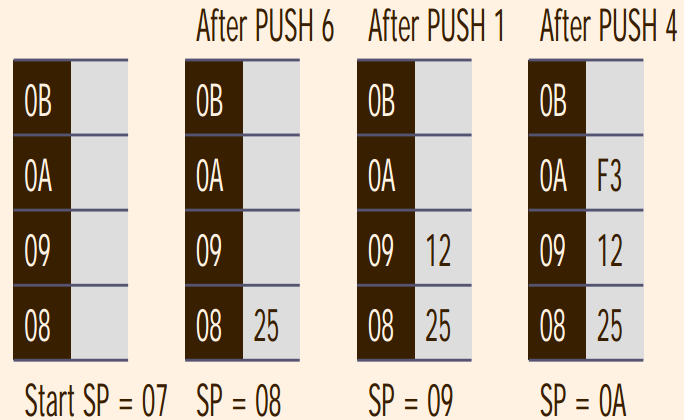
\includegraphics{/home/milav/Codes/MPMC/assets/imgs/181001_MCU_Question_Bank_Solved_html_354d90835c983729.png}
\caption{}
\end{figure}

\begin{enumerate}
\def\labelenumi{\arabic{enumi}.}
\item
  \textbf{POP Instruction:}

  \begin{itemize}
  \item
    \textbf{Retrieves Data:} The POP instruction removes a byte of data
    from the top of the stack.
  \item
    \textbf{SP Modification:}

    \begin{enumerate}
    \def\labelenumii{\arabic{enumii}.}
    \item
      The data at the location pointed to by the SP is retrieved.
    \item
      The SP is then decremented.
    \end{enumerate}
  \end{itemize}
\end{enumerate}

\textbf{POP Example:}

\begin{Shaded}
\begin{Highlighting}[]
\NormalTok{POP R3 ; POP stack into R3}
\NormalTok{POP R5 ; POP stack into R5}
\NormalTok{POP R2 ; POP stack into R2}
\end{Highlighting}
\end{Shaded}

\begin{figure}
\centering
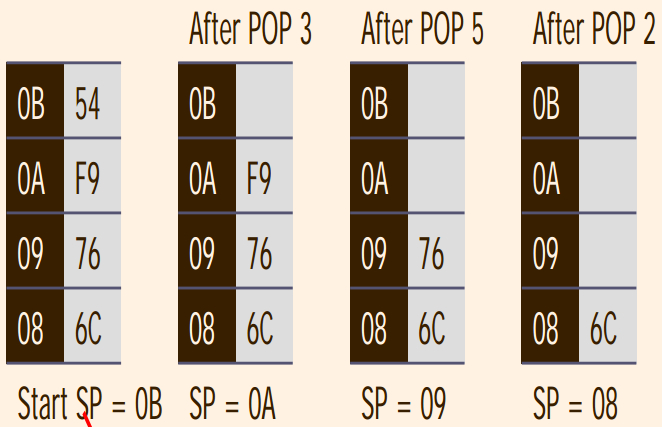
\includegraphics{/home/milav/Codes/MPMC/assets/imgs/181001_MCU_Question_Bank_Solved_html_94d65ad39a469b39.jpg}
\caption{}
\end{figure}

\textbf{Common Uses of the Stack}

\begin{itemize}
\item
  \textbf{Temporary Storage:} Storing the contents of registers during
  calculations when there aren't enough registers available.
\item
  \textbf{Subroutine Calls:} When a subroutine (function) is called
  using the 'CALL' instruction, the return address (next instruction
  after the call) is automatically pushed onto the stack. The 'RET'
  instruction pops this return address, so execution continues
  correctly.
\item
  \textbf{Interrupt Handling:} When an interrupt occurs, the 8051
  automatically pushes the Program Counter (PC) onto the stack, allowing
  seamless return to the interrupted code after the interrupt service
  routine.
\end{itemize}

\textbf{Important Considerations}

\begin{itemize}
\item
  \textbf{Limited Stack Size:} The 8051's internal RAM is small, which
  limits the size of the stack. Be mindful of stack usage to avoid
  overflow conditions.
\item
  \textbf{Stack Overflow:} This occurs if you try to PUSH data when the
  stack is full. This can lead to unpredictable behavior.
\item
  \textbf{Stack Underflow:} This occurs if you try to POP data when the
  stack is empty. This can also result in errors.
\end{itemize}

\begin{itemize}
\item
  \textbf{Stack Size:} The 8051's internal RAM for the stack is limited;
  it's crucial to prevent stack overflow.
\item
  \textbf{Initialization:} The SP is initialized to 07H when the 8051
  resets; your code often needs to set it to a custom location.
\end{itemize}

\textbf{Example: Swapping Two Numbers}

\begin{Shaded}
\begin{Highlighting}[]
\NormalTok{MOV SP, \#70H   ; Initialize Stack Pointer (assuming safe RAM space)}

\NormalTok{MOV A, \#25H    ; Load the first number into the accumulator}
\NormalTok{PUSH A         ; Push the first number onto the stack}

\NormalTok{MOV A, \#30H    ; Load the second number into the accumulator}
\NormalTok{PUSH A         ; Push the second number onto the stack}

\NormalTok{POP B         ; Pop the top (second) number into register B}
\NormalTok{POP A          ; Pop the original (first) number into the accumulator}
\end{Highlighting}
\end{Shaded}

\hypertarget{36-timerscounters}{%
\subsection{3.6. Timers/Counters}\label{36-timerscounters}}

8051 Timers/Counters have two primary modes of operation:

\begin{itemize}
\item
  \textbf{Timer Mode:}

  \begin{itemize}
  \item
    Increments on internal machine cycles.
  \item
    Used to generate time delays or measure time intervals between
    events.
  \end{itemize}
\item
  \textbf{Counter Mode:}

  \begin{itemize}
  \item
    Increments on external pulses applied to designated input pins.
  \item
    Used to count external events, like sensor inputs or rotations of a
    shaft.
  \end{itemize}
\end{itemize}

\textbf{Structure}

\begin{itemize}
\item
  \textbf{Two Timers/Counters:} The 8051 has two flexible 16-bit
  timers/counters, named Timer 0 and Timer 1.
\item
  \textbf{Registers:} Each timer/counter has the following registers:

  \begin{itemize}
  \item
    \textbf{THx and TLx:} "x" denotes the timer number -- Timer 0 (TH0,
    TL0) and Timer 1 (TH1, TL1). These hold the actual timer/counter
    values.
  \item
    \textbf{TMOD:} The Timer Mode register (configuration of modes).
  \item
    \textbf{TCON:} The Timer Control register (start, stop, interrupt
    flags, etc.).
  \end{itemize}
\end{itemize}

\textbf{Applications}

\begin{itemize}
\item
  \textbf{Timing and Delays:} Generating precise delays in code.
\item
  \textbf{Event Counting:} Counting occurrences of external events
  (button presses, sensor triggers, etc.).
\item
  \textbf{PWM (Pulse-Width Modulation):} Used to control the speed of
  motors, brightness of LEDs, etc.
\item
  \textbf{Baud Rate Generation:} Essential for serial communication in
  the 8051.
\item
  \textbf{Real-Time Clock (RTC):} Along with external circuitry, Timers
  can be used to implement an RTC.
\end{itemize}

\textbf{Limitations}

\begin{itemize}
\item
  \textbf{Resolution:} Limited by the 8051's clock speed and the
  timer/counter's 16-bit design. Fine-grained timings and very
  high-frequency counting may be difficult.
\item
  \textbf{Only Two Timers:} Some complex applications might require more
  than the two timers the 8051 provides.
\end{itemize}

\hypertarget{361-tcon-register}{%
\subsubsection{3.6.1. TCON Register}\label{361-tcon-register}}

\textbf{What is the TCON Register?}

\begin{itemize}
\item
  The TCON (Timer Control) register is an 8-bit, bit-addressable
  register present in 8051 microcontrollers.
\item
  It's primarily responsible for controlling the operation of the
  microcontroller's internal timers and counters.
\end{itemize}

\textbf{TCON Register Structure (Address: 088H, Bit addressable)}

\begin{longtable}[]{@{}llllllll@{}}
\toprule
TCON.7 & TCON.6 & TCON.5 & TCON.4 & TCON.3 & TCON.2 & TCON.1 & TCON.0 \\
\midrule
\endhead
TF1 & TR1 & TF0 & TR0 & IE1 & IT1 & IE0 & IT0 \\
\bottomrule
\end{longtable}

The 8 bits of the TCON register are assigned specific functions:

\begin{itemize}
\item
  \textbf{TF1 (Timer 1 Overflow Flag):} Set to '1' when Timer 1
  overflows. Cleared by software.
\item
  \textbf{TR1 (Timer 1 Run Control Bit):} Controls the Run/Stop status
  of Timer 1.

  \begin{itemize}
  \item
    '1' = Timer 1 is running
  \item
    '0' = Timer 1 is stopped
  \end{itemize}
\item
  \textbf{TF0 (Timer 0 Overflow Flag):} Set to '1' when Timer 0
  overflows. Cleared by software.
\item
  \textbf{TR0 (Timer 0 Run Control Bit):} Controls the Run/Stop status
  of Timer 0.

  \begin{itemize}
  \item
    '1' = Timer 0 is running
  \item
    '0' = Timer 0 is stopped
  \end{itemize}
\item
  \textbf{IE1 (External Interrupt 1 Edge Flag):} Set to '1' when an
  external interrupt 1 occurs on a falling edge transition. Cleared by
  software.
\item
  \textbf{IT1 (External Interrupt 1 Type Control Bit):} Configures
  external interrupt 1 trigger type.

  \begin{itemize}
  \item
    '1' = Falling edge triggered
  \item
    '0' = Low-level triggered.
  \end{itemize}
\item
  \textbf{IE0 (External Interrupt 0 Edge Flag):} Set to '1' when an
  external interrupt 0 occurs on a falling edge transition. Cleared by
  software.
\item
  \textbf{IT0 (External Interrupt 0 Type Control Bit):} Configures
  external interrupt 0 trigger type.

  \begin{itemize}
  \item
    '1' = Falling edge triggered
  \item
    '0' = Low-level triggered
  \end{itemize}
\end{itemize}

\begin{longtable}[]{@{}ll@{}}
\toprule
Flag & Function \\
\midrule
\endhead
TF1 & Timer 1 Overflow flag. Set when timer rolls from all 1's to 0.
Cleared when processor vectors to execute interrupt service routine
located at program address 001Bh. \\
TR1 & Timer 1 run control bit. Set to 1 by program to enable timer to
count; cleared to 0 by program to halt timer. \\
TF0 & Timer 0 Overflow flag. Set when timer rolls from all 1's to 0.
Cleared when processor vectors to execute interrupt service routine
located at program address 000Bh. \\
TR0 & Timer 0 run control bit. Set to 1 by program to enable timer to
count; cleared to 0 by program to halt timer. \\
IE1 & External interrupt 1 Edge flag. Set to 1 when a high-to-low edge
signal is received on port 3.3 (INT1). Cleared when processor vectors to
interrupt service routine at program address 0013h. Not related to timer
operations. \\
IT1 & External interrupt 1 signal type control bit. Set to 1 by program
to enable external interrupt 1 to be triggered by a falling edge signal.
Set to 0 by program to enable a low-level signal on external interrupt 1
to generate an interrupt. \\
IE0 & External interrupt 0 Edge flag. Set to 1 when a high-to-low edge
signal is received on port 3.2 (INT0). Cleared when processor vectors to
interrupt service routine at program address 0003h. Not related to timer
operations. \\
IT0 & External interrupt 0 signal type control bit. Set to 1 by program
to enable external interrupt 1 to be triggered by a falling edge signal.
Set to 0 by program to enable a low-level signal on external interrupt 0
to generate an interrupt. \\
\bottomrule
\end{longtable}

\textbf{Key Functions of TCON Register}

\begin{enumerate}
\def\labelenumi{\arabic{enumi}.}
\item
  \textbf{Timer/Counter Start/Stop:} The TR1 and TR0 bits enable you to
  start and stop Timer 1 and Timer 0, respectively.
\item
  \textbf{Overflow Monitoring:} The overflow flags TF1 and TF0 indicate
  when a timer has reached its maximum count and rolled over. These are
  often used to generate interrupts.
\item
  \textbf{External Interrupt Configuration:} The IE0, IT0, IE1, and IT1
  bits control how external interrupts are triggered and detected by the
  microcontroller.
\end{enumerate}

\textbf{Example: Setting up Timer 0 as an interval timer}

\begin{enumerate}
\def\labelenumi{\arabic{enumi}.}
\item
  \textbf{Set the Mode:} To use Timer 0 in a specific mode, you'll
  configure the TMOD register (Timer Mode Register). Let's assume you
  want Timer 0 as a 16-bit interval timer.
\item
  \textbf{Load Initial Value:} Load the desired starting count into the
  TH0 (Timer 0 High Byte) and TL0 (Timer 0 Low Byte) registers.
\item
  \textbf{Start the Timer:} Set TR0 (Timer 0 Run Control Bit) in the
  TCON register to '1' to begin the timer.
\item
  \textbf{Interrupt Handling (Optional):} If you want an interrupt to be
  generated when the timer overflows, set the interrupt enable bits in
  relevant registers and create an interrupt service routine (ISR). The
  TF0 flag in TCON will be set when an overflow occurs.
\end{enumerate}

\hypertarget{362-tmod-register}{%
\subsubsection{3.6.2. TMOD Register}\label{362-tmod-register}}

\textbf{What is the TMOD Register?}

\begin{itemize}
\item
  The TMOD (Timer Mode) register is an 8-bit, bit-addressable Special
  Function Register (SFR) within 8051 microcontrollers.
\item
  Its primary role is to select and configure the operating modes of the
  two built-in timers: Timer 0 and Timer 1.
\end{itemize}

\textbf{TMOD Register Structure (Address: 089H, Bit addressable):}

\begin{longtable}[]{@{}llllllll@{}}
\toprule
TMOD.7 & TMOD.6 & TMOD.5 & TMOD.4 & TMOD.3 & TMOD.2 & TMOD.1 & TMOD.0 \\
\midrule
\endhead
Timer1 GATE & Timer1 C/T & Timer1 M1 & Timer1 M0 & Timer0 GATE & Timer0
C/T & Timer0 M1 & Timer0 M0 \\
\bottomrule
\end{longtable}

The TMOD register has a specific function assigned to each of its 8
bits:

\begin{itemize}
\item
  \textbf{Bits 7-4 (Timer 1 Configuration)}

  \begin{itemize}
  \item
    \textbf{Gate:} Controls Timer 1 gating for external control
    (described later).
  \item
    \textbf{C/T̄:} Selects Timer vs. Counter mode for Timer 1.

    \begin{itemize}
    \item
      '1' = Counter mode (counts external pulses)
    \item
      '0' = Timer mode (counts internal machine cycles)
    \end{itemize}
  \item
    \textbf{M1 M0:} Selects the operating mode of Timer 1 (Modes 0, 1,
    2, or 3)
  \end{itemize}
\item
  \textbf{Bits 3-0 (Timer 0 Configuration)}: Same structure as Timer 1
  configuration bits above, but control the settings for Timer 0.
\end{itemize}

\begin{longtable}[]{@{}ll@{}}
\toprule
Bit & Function \\
\midrule
\endhead
Timer1 GATE & GATE enables and disables Timer by means of a signal
brought to the INTx pin: 1 -- Timer operates only if the INTx bit is
set. 0 -- Timer operates regardless of the logic state of the INTx
bit. \\
Timer1 C/T & C/T selects pulses to be counted up by the timer/counter: 1
-- Timer counts pulses brought to the Tx(Timer) pin. 0 -- Timer counts
pulses from the internal oscillator. \\
Timer1 M1 & M1, M0 These two bits select the operational mode Timer. \\
Timer1 M0 & M1, M0 These two bits select the operational mode Timer. \\
Timer0 GATE & GATE enables and disables Timer by means of a signal
brought to the INTx pin: 1 -- Timer operates only if the INTx bit is
set. 0 -- Timer operates regardless of the logic state of the INTx
bit. \\
Timer0 C/T & C/T selects pulses to be counted up by the timer/counter: 1
-- Timer counts pulses brought to the Tx(Timer) pin. 0 -- Timer counts
pulses from the internal oscillator. \\
Timer0 M1 & M1, M0 These two bits select the operational mode Timer. \\
Timer0 M0 & M1, M0 These two bits select the operational mode Timer. \\
\bottomrule
\end{longtable}

\textbf{Operating Modes}

\begin{longtable}[]{@{}llll@{}}
\toprule
M1 & M0 & Mode & Operating Mode \\
\midrule
\endhead
0 & 0 & 0 & 13-bit Mode \\
0 & 1 & 1 & 16-bit Mode \\
1 & 0 & 2 & 8-bit Auto Reaload Mode \\
1 & 1 & 3 & Split Timer Mode \\
\bottomrule
\end{longtable}

The TMOD register allows you to configure each timer into one of four
operating modes:

\begin{itemize}
\item
  \textbf{Mode 0 (13-bit Timer):}

  \begin{itemize}
  \item
    Timer register is effectively 13 bits (THx: 8 bits, TLx: 5 bits)
  \item
    This mode is often used for simple timing or event counting where
    extremely long delays are not required.
  \end{itemize}
\item
  \textbf{Mode 1 (16-bit Timer):}

  \begin{itemize}
  \item
    The standard 16-bit timer/counter mode, providing the full range of
    counting.
  \end{itemize}
\item
  \textbf{Mode 2 (8-bit Auto-Reload Timer):}

  \begin{itemize}
  \item
    TLx is reloaded with the value in THx automatically after each
    overflow. Useful for generating fixed periodic events.
  \end{itemize}
\item
  \textbf{Mode 3 (Split Timer):}

  \begin{itemize}
  \item
    Timer 1 is stopped. TL0 is used as an 8-bit Timer/Counter and can be
    controlled independently, while TH0 runs as a separate 8-bit timer
    (usually controlled by the system clock).
  \end{itemize}
\end{itemize}

\textbf{Gate Bit}

The Gate bit for each timer provides additional control:

\begin{itemize}
\item
  \textbf{Gate = '0':} The timer runs continuously when the TRx bit (in
  TCON) is set to '1'.
\item
  \textbf{Gate = '1':} The timer runs only when the TRx bit is '1' AND
  an external pin (INT0 or INT1) receives a high-to-low transition.
\end{itemize}

\textbf{Example: Configuring Timer 0 as a 16-bit timer with gating}

\begin{enumerate}
\def\labelenumi{\arabic{enumi}.}
\item
  \textbf{Setting the Mode:} To configure Timer 0 as a 16-bit timer, set
  the corresponding bits in the TMOD register as follows:

\begin{Shaded}
\begin{Highlighting}[]
\NormalTok{TMOD = 0x01; // Assuming you want Timer 0 in Mode 1, Timer 1 is not important here}
\end{Highlighting}
\end{Shaded}
\item
  \textbf{Enabling Gating:} If you want to control Timer 0 with an
  external signal on INT0 pin:

\begin{Shaded}
\begin{Highlighting}[]
\NormalTok{TMOD |= 0x08; // Set the Gate bit for Timer 0}
\end{Highlighting}
\end{Shaded}
\end{enumerate}

\hypertarget{363-modes-of-operation}{%
\subsubsection{3.6.3. Modes of Operation}\label{363-modes-of-operation}}

\textbf{Mode 0: 13-Bit Timer}

\begin{itemize}
\item
  \textbf{Configuration:} The timer register is split into two parts:

  \begin{itemize}
  \item
    Five high-order bits (THx)
  \item
    Eight low-order bits (TLx), with the top 3 bits of TLx written as
    zeroes.
  \end{itemize}
\item
  \textbf{Operation:} The 5 bits of TLx are automatically incremented.
  When TLx overflows, it increments THx. This forms a 13-bit timer.
\item
  \textbf{Use Cases:} Often used for event counting or generating baud
  rates in serial communication, particularly when interfacing with
  legacy systems.
\end{itemize}

\textbf{Mode 1: 16-Bit Timer}

\begin{itemize}
\item
  \textbf{Configuration:} The full 16-bits of the Timer register (THx
  and TLx) function as a single timer unit.
\item
  \textbf{Operation:} Each clock pulse increments the entire register.
\item
  \textbf{Use Cases} General-purpose time delays, long interval
  measurements, anything requiring 16-bit precision timing.
\end{itemize}

\textbf{Mode 2: 8-Bit Auto-Reload Timer}

\begin{itemize}
\item
  \textbf{Configuration:}

  \begin{itemize}
  \item
    THx holds a fixed reload value.
  \item
    TLx operates as the 8-bit timer.
  \end{itemize}
\item
  \textbf{Operation:}

  \begin{itemize}
  \item
    TLx counts up. When it overflows, it's automatically reloaded with
    the value stored in THx.
  \item
    This creates a recurring time interval.
  \end{itemize}
\item
  \textbf{Use Cases:} Generating fixed, predictable time delays or
  timing periodic events.
\end{itemize}

\textbf{Mode 3: Split 8-bit Timers}

\begin{itemize}
\item
  \textbf{Configuration:}

  \begin{itemize}
  \item
    Timer 0 is split into two independent 8-bit timers/counters: TL0 and
    TH0.
  \item
    Timer 1 remains as a 16-bit timer if needed.
  \end{itemize}
\item
  \textbf{Operation:}

  \begin{itemize}
  \item
    TL0 and TH0 function as two separate timers, often with TL0 used as
    a timer and TH0 used as a counter.
  \end{itemize}
\item
  \textbf{Use Cases:}

  \begin{itemize}
  \item
    Situations requiring two independent timers
  \item
    Generating baud rates (TL0) while counting external events (TH0)
  \end{itemize}
\end{itemize}

\textbf{Key Control Registers}

\begin{itemize}
\item
  \textbf{TMOD (Timer Mode):} This register selects the operating mode
  for Timer 0 and Timer 1.
\item
  \textbf{TCON (Timer Control):} Contains flags and start/stop control
  bits for the timers.
\end{itemize}

\textbf{How to Select a Mode}

Mode selection depends on:

\begin{itemize}
\item
  \textbf{Timing Precision:} 16-bit vs. 8-bit
\item
  \textbf{Recurring Intervals:} Auto-reload mode vs. manual restart.
\item
  \textbf{Number of Timers Needed:} Split timer mode provides two
  independent 8-bit timers if needed within Timer 0.
\end{itemize}

\hypertarget{3631-timer-mode-0-13-bit-timer-mode}{%
\paragraph{3.6.3.1. Timer Mode 0 (13-bit Timer
Mode)}\label{3631-timer-mode-0-13-bit-timer-mode}}

\begin{itemize}
\item
  \textbf{Split Registers:} In Mode 0, each timer's 16-bit register is
  effectively split into:

  \begin{itemize}
  \item
    \textbf{THx (8 bits):} Holds the upper 8 bits of the timer count.
  \item
    \textbf{TLx (5 bits):} Holds the lower 5 bits of the timer count.
  \end{itemize}
\item
  \textbf{Counter Behavior:} Only TLx is actually incremented. Whenever
  TLx overflows (reaches 32 counts), it's reset to zero, and THx is
  incremented by one.
\item
  \textbf{Effective Count:} This provides a 13-bit count. The maximum
  count is effectively 8192 (2\^{}13).
\end{itemize}

\textbf{Key Points about Mode 0}

\begin{itemize}
\item
  \textbf{Timer vs. Counter:} Mode 0 can be used as either a timer
  (counting internal machine cycles) or as a counter (counting external
  pulses). This is controlled by the C/T̄ bit in the TMOD register.
\item
  \textbf{Limited Range:} Due to the 13-bit design, Mode 0 is primarily
  useful for relatively short delays or event counting where extremely
  long intervals are not required.
\end{itemize}

\begin{figure}
\centering

\includegraphics{/home/milav/Codes/MPMC/assets/imgs/181001_MCU_Question_Bank_Solved_html_aa0c251bc1971fd3.png}
\caption{}
\end{figure}

\textbf{Example: Creating a Delay Using Timer 0 in Mode 0}

Assuming you have a 12 MHz crystal oscillator for your 8051 (1 machine
cycle = 1 microsecond):

\begin{enumerate}
\def\labelenumi{\arabic{enumi}.}
\item
  \textbf{Mode Setup:}

\begin{Shaded}
\begin{Highlighting}[]
\NormalTok{TMOD }\OperatorTok{=} \BaseNTok{0x01}\OperatorTok{;}  \CommentTok{// Set Timer 0 in Mode 0 (13{-}bit timer)}
\end{Highlighting}
\end{Shaded}
\item
  \textbf{Calculate Delay Value:}

  \begin{itemize}
  \item
    Let's say you want a 50-millisecond (0.05 seconds) delay.
  \item
    We need 50000 machine cycles (50,000 microseconds).
  \item
    Because the timer counts up, calculate the value to subtract from
    the max value: 8192 - 50000 = -41808.
  \item
    Since the counter is unsigned, the 16-bit representation of -41808
    is 3CAF (hex).
  \end{itemize}
\item
  \textbf{Load Timer Registers:}

\begin{Shaded}
\begin{Highlighting}[]
\NormalTok{TH0 }\OperatorTok{=} \BaseNTok{0x3C}\OperatorTok{;}
\NormalTok{TL0 }\OperatorTok{=} \BaseNTok{0xAF}\OperatorTok{;}
\end{Highlighting}
\end{Shaded}
\item
  \textbf{Start Timer:}

\begin{Shaded}
\begin{Highlighting}[]
\NormalTok{TR0 }\OperatorTok{=} \DecValTok{1}\OperatorTok{;} \CommentTok{// Set the TR0 bit in TCON to start Timer 0}
\end{Highlighting}
\end{Shaded}
\item
  \textbf{Wait for Overflow:}

\begin{Shaded}
\begin{Highlighting}[]
\ControlFlowTok{while} \OperatorTok{(}\NormalTok{TF0 }\OperatorTok{==} \DecValTok{0}\OperatorTok{);} \CommentTok{// Wait for the Timer 0 Overflow flag (TF0 in TCON) to be set}
\NormalTok{TR0 }\OperatorTok{=} \DecValTok{0}\OperatorTok{;} \CommentTok{// Stop the timer}
\NormalTok{TF0 }\OperatorTok{=} \DecValTok{0}\OperatorTok{;} \CommentTok{// Clear the overflow flag}
\end{Highlighting}
\end{Shaded}
\end{enumerate}

\textbf{Explanation}

The timer will start counting up from 0x3CAF. After 41808 machine
cycles, an overflow will occur, setting TF0 to '1'. Your code detects
this and stops the timer. You have now generated your desired
50-millisecond delay.

\hypertarget{3632-timer-mode-1-16-bit-timer-mode}{%
\paragraph{3.6.3.2. Timer Mode 1 (16-bit Timer
Mode)}\label{3632-timer-mode-1-16-bit-timer-mode}}

\begin{itemize}
\item
  \textbf{Full 16-bit Register:} In Mode 1, both THx and TLx registers
  of a timer act as a single 16-bit register.
\item
  \textbf{Counting:} The 16-bit register is incremented on each timer
  pulse (either internal machine cycles or external pulses, depending on
  the C/T̄ bit in TMOD).
\item
  \textbf{Maximum Count:} Timers in Mode 1 can count up to the full
  16-bit range, which is 65,536.
\end{itemize}

\begin{figure}
\centering
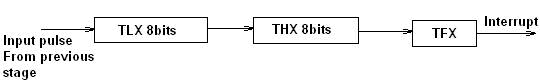
\includegraphics{/home/milav/Codes/MPMC/assets/imgs/181001_MCU_Question_Bank_Solved_html_d97c58ff97348292.png}
\caption{}
\end{figure}

\textbf{Example: Generating a 1-Second Delay with Timer 0 in Mode 1}

Let's assume a 12 MHz crystal oscillator (1 machine cycle = 1
microsecond):

\begin{enumerate}
\def\labelenumi{\arabic{enumi}.}
\item
  \textbf{Mode Setup:}

\begin{Shaded}
\begin{Highlighting}[]
\NormalTok{MOV TMOD, \#01H ; Set Timer 0 in Mode 1 (16{-}bit timer)}
\end{Highlighting}
\end{Shaded}
\item
  \textbf{Calculating the Reload Value:}

  \begin{itemize}
  \item
    We need a 1-second delay (1,000,000 microseconds).
  \item
    Since the timer increments on each machine cycle, we need 1,000,000
    counts.
  \item
    To create a delay, we subtract this from the max count and load the
    result: 65536 - 1000000 = -934464
  \item
    As the counter is unsigned, the 16-bit representation is FC18 (hex).
  \end{itemize}
\item
  \textbf{Loading Timer Registers:}

\begin{Shaded}
\begin{Highlighting}[]
\NormalTok{MOV TH0, \#0FCH ; Load the high byte of the reload value}
\NormalTok{MOV TL0, \#18H  ; Load the low byte of the reload value}
\end{Highlighting}
\end{Shaded}
\item
  \textbf{Starting the Timer:}

\begin{Shaded}
\begin{Highlighting}[]
\NormalTok{SETB TR0 ; Start Timer 0}
\end{Highlighting}
\end{Shaded}
\item
  \textbf{Waiting for Overflow:}

\begin{Shaded}
\begin{Highlighting}[]
\NormalTok{JNB TF0, $  ; Keep checking the Timer 0 Overflow flag (TF0 in TCON) and jump back to this line if not yet set}
\NormalTok{CLR TR0    ; Stop the timer}
\NormalTok{CLR TF0    ; Clear the overflow flag}
\end{Highlighting}
\end{Shaded}
\end{enumerate}

\textbf{Explanation}

\begin{itemize}
\item
  The timer starts counting from FC18. When it reaches FFFF, it
  overflows, setting the TF0 flag to '1'.
\item
  The \texttt{JNB\ TF0,\ \$} instruction creates a loop that checks the
  TF0 flag, effectively waiting for the overflow.
\item
  Once the overflow occurs, the timer is stopped, and the flag is
  cleared.
\end{itemize}

\textbf{Important Notes:}

\begin{itemize}
\item
  The C/T̄ bit in the TMOD register determines whether the timer counts
  internal machine cycles (timer mode) or external pulses (counter
  mode).
\item
  Mode 1 is the most common mode for timers in 8051 microcontrollers due
  to its flexibility and larger counting range.
\end{itemize}

\hypertarget{3633-timer-mode-2-8-bit-auto-reload-timer-mode}{%
\paragraph{3.6.3.3. Timer Mode 2 (8-bit Auto-Reload Timer
Mode)}\label{3633-timer-mode-2-8-bit-auto-reload-timer-mode}}

\begin{itemize}
\item
  \textbf{Key Feature:} In Mode 2, the TLx register acts as the timer
  itself, while the THx register holds a reload value.
\item
  \textbf{Auto-Reload Behavior:}

  \begin{itemize}
  \item
    TLx counts up.
  \item
    When TLx overflows from FFH to 00H, it's automatically reloaded with
    the value stored in THx.
  \item
    This cycle repeats, generating a continuous timer.
  \end{itemize}
\end{itemize}

\textbf{Advantages of Mode 2}

\begin{itemize}
\item
  \textbf{Fixed-Period Generation:} Mode 2 is ideal for generating
  fixed-period delays or timing events without requiring software
  intervention to reload the timer after each cycle.
\item
  \textbf{Baud Rate Generation:} Mode 2 is often used in serial
  communication to create a reliable clock for baud rate generation.
\end{itemize}

\begin{figure}
\centering
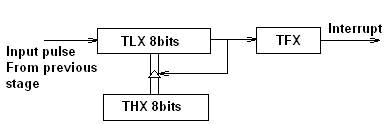
\includegraphics{/home/milav/Codes/MPMC/assets/imgs/181001_MCU_Question_Bank_Solved_html_a63407a2fb9d9df6.png}
\caption{}
\end{figure}

\textbf{Example: Creating a Square Wave with 50\% Duty Cycle on Timer 1}

Assumptions:

\begin{itemize}
\item
  12 MHz crystal oscillator.
\item
  Desired square wave frequency: 1 kHz (period = 1 millisecond).
\end{itemize}

\begin{enumerate}
\def\labelenumi{\arabic{enumi}.}
\item
  \textbf{Mode Setup:}

\begin{Shaded}
\begin{Highlighting}[]
\NormalTok{MOV TMOD, \#20H ; Set Timer 1 in Mode 2 (8{-}bit auto{-}reload)}
\end{Highlighting}
\end{Shaded}
\item
  \textbf{Calculating Reload Value:}

  \begin{itemize}
  \item
    A 1 kHz wave with a 50\% duty cycle requires a 0.5 millisecond
    on-time and a 0.5 millisecond off-time.
  \item
    0.5 ms corresponds to 6000 machine cycles (0.5 ms * 12,000
    cycles/ms).
  \item
    To make the timer count for 6000 cycles, we need to load the reload
    value with 256 - 6000 = -5744.
  \item
    The 8-bit representation of -5744 is DAH (hex).
  \end{itemize}
\item
  \textbf{Loading TH1:}

\begin{Shaded}
\begin{Highlighting}[]
\NormalTok{MOV TH1, \#0DAH ; Load the reload value}
\end{Highlighting}
\end{Shaded}
\item
  \textbf{Starting the Timer:}

\begin{Shaded}
\begin{Highlighting}[]
\NormalTok{SETB TR1 ; Start Timer 1}
\end{Highlighting}
\end{Shaded}
\item
  \textbf{Generating the Square Wave (Hardware handles most of this):}

  \begin{itemize}
  \item
    Connect an output pin of your microcontroller to the T1 pin (P3.4)
    for the 8051.
  \end{itemize}
\end{enumerate}

\textbf{Explanation}

\begin{itemize}
\item
  Timer 1 will begin counting up from 00H. When it reaches FFH, it
  overflows, automatically reloads with DAH from TH1, and the process
  repeats.
\item
  The hardware of the 8051 will automatically toggle the T1 pin on each
  overflow, creating the square wave output.
\end{itemize}

\textbf{Important Notes}

\begin{itemize}
\item
  Mode 2 is exclusively a timer mode -- it always counts internal
  machine cycles.
\item
  You can adjust the duty cycle of the square wave in the example by
  changing the reload value loaded into TH1.
\end{itemize}

\hypertarget{3634-timer-mode-3-split-timer-mode}{%
\paragraph{3.6.3.4. Timer Mode 3 (Split Timer
Mode)}\label{3634-timer-mode-3-split-timer-mode}}

Mode 3 is a unique mode for Timer 0 and Timer 1 with specific behaviors:

\textbf{Timer 0 in Mode 3}

\begin{itemize}
\item
  \textbf{TL0 (8-bit Timer/Counter):} Behaves as a standard 8-bit timer
  or counter, controlled by the C/T̄ bit in TMOD and the TR0 bit in TCON.
\item
  \textbf{TH0 (8-bit Timer):} Acts as an independent timer, usually
  controlled by the system clock (machine cycles). It is not affected by
  TR0 in this mode.
\end{itemize}

\textbf{Timer 1 in Mode 3}

\begin{itemize}
\item
  \textbf{Stopped:} Timer 1 is essentially halted in Mode 3.
\item
  \textbf{Control Bits:} Timer 1's control bits (TR1 and TF1) are used
  instead by Timer 0. This allows Timer 0 to be gated (controlled by an
  external signal).
\end{itemize}

\textbf{Why is Mode 3 Useful?}

\begin{enumerate}
\def\labelenumi{\arabic{enumi}.}
\item
  \textbf{Extra Timer:} Mode 3 gives you an additional 8-bit timer (TH0)
  if you need more than the standard two timers that the 8051 provides.
\item
  \textbf{Gating Timer 0:} It allows you to control the Start/Stop of
  Timer 0 with an external signal on the INT0 pin, providing more
  flexible control for timing operations.
\end{enumerate}

\begin{figure}
\centering
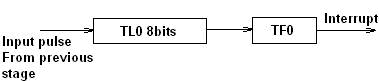
\includegraphics{/home/milav/Codes/MPMC/assets/imgs/181001_MCU_Question_Bank_Solved_html_9d69089b6ba947bf.png}
\caption{}
\end{figure}

\textbf{Example: Using Timer 0 in Mode 3 as a Gated Timer}

Let's assume you want Timer 0 to count external events on pin INT0 and
TH0 to generate a time base.

\begin{enumerate}
\def\labelenumi{\arabic{enumi}.}
\item
  \textbf{Mode Setup:}

\begin{Shaded}
\begin{Highlighting}[]
\NormalTok{MOV TMOD, \#09H ; Set Timer 0 in Mode 3, Timer 1 is not important in this case}
\end{Highlighting}
\end{Shaded}
\item
  \textbf{Gating Setup:}

\begin{Shaded}
\begin{Highlighting}[]
\NormalTok{SETB GATE  ; Enable gating for Timer 0 in TCON. This means TR0 alone won\textquotesingle{}t start the timer}
\end{Highlighting}
\end{Shaded}
\item
  \textbf{Using the Functionality}

  \begin{itemize}
  \item
    \textbf{TL0:} Will now count pulses received on the INT0 pin.
  \item
    \textbf{TH0:} Will count machine cycles and can be used for
    independent timing operations.
  \item
    \textbf{To start Timer 0:} Ensure TR0 is set to '1' AND a
    high-to-low transition occurs on the INT0 pin.
  \end{itemize}
\end{enumerate}

\textbf{Key Points}

\begin{itemize}
\item
  Mode 3 for Timer 1 is rarely used directly; its primary purpose is to
  give Timer 0 the extra control features.
\item
  Timer 0 needs both TR0 = '1' and the external gating signal for it to
  function when in Mode 3.
\end{itemize}

\hypertarget{37-serial-communication}{%
\subsection{3.7. Serial Communication}\label{37-serial-communication}}

\textbf{What is Serial Communication?}

\begin{itemize}
\item
  Serial communication is a method of transmitting data between devices
  where the bits of data are sent sequentially over a single
  communication line or channel. This contrasts with parallel
  communication where multiple bits are sent at the same time over
  multiple lines.
\end{itemize}

\textbf{Key Modes of Serial Communication}

\begin{enumerate}
\def\labelenumi{\arabic{enumi}.}
\item
  \textbf{Simplex Mode}

  \begin{itemize}
  \item
    \textbf{Unidirectional transmission:} Data flows in only one
    direction, from the transmitter to the receiver.
  \item
    \textbf{Example:} A TV broadcasting station transmits signals to
    countless television sets (receivers). TVs can't transmit back to
    the station.
  \end{itemize}
\item
  \textbf{Half-Duplex Mode}

  \begin{itemize}
  \item
    \textbf{Bidirectional, but not simultaneous:} Both devices can
    transmit and receive, but not at the same time. They must take
    turns.
  \item
    \textbf{Example:} Walkie-talkies. A user presses a button to talk
    (transmit) and releases the button to listen (receive). Both users
    cannot talk at the same time.
  \end{itemize}
\item
  \textbf{Full-Duplex Mode}

  \begin{itemize}
  \item
    \textbf{Simultaneous bidirectional transmission:} Both devices can
    transmit and receive data at the same time.
  \item
    \textbf{Example:} Modern phone calls. Both parties can talk and
    listen simultaneously.
  \end{itemize}
\end{enumerate}

\textbf{Asynchronous vs. Synchronous Communication}

Within serial communication, there's an important distinction between
asynchronous and synchronous modes:

\begin{itemize}
\item
  \textbf{Asynchronous:}

  \begin{itemize}
  \item
    No shared clock signal between devices.
  \item
    Data is framed using start and stop bits to signal the beginning and
    end of a data packet.
  \item
    Good for irregular data transmission with potential gaps between
    bytes.
  \end{itemize}
\item
  \textbf{Synchronous:}

  \begin{itemize}
  \item
    Devices share a clock signal that synchronizes the timing of data
    transmission.
  \item
    Data bytes flow in a continuous stream without the need for start
    and stop bits.
  \item
    Ideal for high-speed, continuous data transmission.
  \end{itemize}
\end{itemize}

\textbf{Example: UART Communication (Typically Asynchronous)}

\begin{itemize}
\item
  \textbf{Hardware:} A Universal Asynchronous Receiver/Transmitter
  (UART) is a common hardware component for serial communication.
\item
  \textbf{Protocol:} Data is framed with a start bit, 5-9 data bits, an
  optional parity bit (for error checking), and one or more stop bits.
\item
  \textbf{Transmission:}

  \begin{itemize}
  \item
    The transmitter sends out the start bit (logic low)
  \item
    Data bits are sent one by one (least significant bit first)
  \item
    Parity bit (if used) is sent
  \item
    Stop bit (logic high) signals packet's end
  \end{itemize}
\item
  \textbf{Example Use Case:} Computer sending commands to a
  microcontroller over a serial connection.
\end{itemize}

\textbf{Note:} Other serial protocols exist, such as SPI (Serial
Peripheral Interface) and I2C (Inter-Integrated Circuit), each with
specific features and applications.

\hypertarget{371-scon-register}{%
\subsubsection{3.7.1. SCON Register}\label{371-scon-register}}

\textbf{What is the SCON Register?}

\begin{itemize}
\item
  The SCON (Serial Control) register is an 8-bit, bit-addressable
  Special Function Register (SFR) responsible for managing serial
  communication in 8051 microcontrollers.
\item
  It holds settings and status flags that control how the
  microcontroller sends and receives data serially.
\end{itemize}

\textbf{SCON Register Structure (Address: 098H, Bit addressable):}

\begin{longtable}[]{@{}llllllll@{}}
\toprule
SCON.7 & SCON.6 & SCON.5 & SCON.4 & SCON.3 & SCON.2 & SCON.1 & SCON.0 \\
\midrule
\endhead
SM0 & SM1 & SM2 & REN & TB8 & RB8 & TI & RI \\
\bottomrule
\end{longtable}

Here's how the SCON register's bits function:

\begin{itemize}
\item
  \textbf{SM0, SM1 (Serial Mode Selection Bits):} These bits define the
  serial communication mode for the 8051. There are four primary modes:

  \begin{itemize}
  \item
    \textbf{Mode 0:} 8-bit shift register for serial port output, clock
    for serial port input is generated internally.
  \item
    \textbf{Mode 1:} 10-bit UART mode (8 data bits, 1 start bit, 1 stop
    bit).
  \item
    \textbf{Mode 2:} 11-bit UART mode (8 data bits, 1 start bit, 1
    programmable stop bit, 1 additional bit for addressing or other
    purposes)
  \item
    \textbf{Mode 3:} Similar to mode 2, but with 9 data bits.
  \end{itemize}

  \begin{longtable}[]{@{}lllll@{}}
  \toprule
  SMO & SM1 & Mode & Baud Rate & Description \\
  \midrule
  \endhead
  0 & 0 & Mode 0 & Fixed Baud Rate (fosc/12) & 8-Bit Synchronous Shift
  Register Mode \\
  0 & 1 & Mode 1 & Variable Baud Rate (Can be set by Timer 1) & 8-bit
  Standard UART mode \\
  1 & 0 & Mode 2 & Fixed Baud Rate (fosc/64) or (fosc/32) & 9-bit
  Multiprocessor Comm. mode \\
  1 & 1 & Mode 3 & Variable Baud Rate (Can be set by Timer 1) & 9-bit
  Multiprocessor Comm. mode \\
  \bottomrule
  \end{longtable}
\item
  \textbf{SM2 (Enable Multiprocessor Communication):} Specifically
  designed for multiprocessor systems to distinguish between data from
  other processors and address information.
\item
  \textbf{REN (Receive Enable):}

  \begin{itemize}
  \item
    '1' = Enables serial reception
  \item
    '0' = Disables serial reception.
  \end{itemize}
\item
  \textbf{TB8 (Transmit Bit 8):} In Modes 2 and 3, this is the 9th data
  bit that is transmitted.
\item
  \textbf{RB8 (Receive Bit 8):} There are two interpretations:

  \begin{itemize}
  \item
    Modes 1, 2, and 3: This is the 9th data bit received.
  \item
    Mode 0: RB8 becomes the stop bit when received.
  \end{itemize}
\item
  \textbf{TI (Transmit Interrupt Flag):}

  \begin{itemize}
  \item
    '1' = Signals that the transmit buffer is empty, ready for new data
    (set by hardware).
  \item
    '0' = Transmission is in progress (cleared by software).
  \end{itemize}
\item
  \textbf{RI (Receive Interrupt Flag):}

  \begin{itemize}
  \item
    '1' = Signals that the receive buffer is full (set by hardware).
  \item
    '0' = No data in the buffer to be read (cleared by software).
  \end{itemize}
\end{itemize}

\begin{longtable}[]{@{}ll@{}}
\toprule
Bit & Function \\
\midrule
\endhead
SM0 & These 2 bits determine the framing of data by specifying number of
bits per \\
SM1 & character and start and stop bits. they take following
combo.SM0 \\
SM2 & This enables multiprocessing capabilities of 8051. Usually set to
0 \\
REN & Also referred to as SCON.4 as SCON is a bit addressable register.
This is receive enable. When high or 1 it allows 8051 to receive data
from RxD pin. Used or access as SET SCON.4 and CLR SCON.4. very useful
in blocking external serial reception. \\
TB8 & Transfer bit 8. Used for serial mode 2 and 3 not generally used so
set it always to 0 \\
RB8 & Receive bit 8. Again used for serial mode 2 and 3 not used so set
it to 0 \\
TI & Transmit interrupt. Important flag bit in SCON register. When 8051
finishes transfer of 8 bit character, it raises the T1 flag to indicate
that it is ready to transfer another byte. Is used at beginning of stop
bit. \\
RI & Receive interrupt. Another important flag bit in SCON register.
When 8051 finishes receiving data i.e when data is successfully stored
in SBUF it raises R1 flag to indicate byte is received and to be picked
before it gets lost. \\
\bottomrule
\end{longtable}

\textbf{Example: Setting up Serial Communication in Mode 1 (10-bit
UART)}

\begin{enumerate}
\def\labelenumi{\arabic{enumi}.}
\item
  \textbf{Mode Selection:} Set the SM0 and SM1 bits in the SCON
  register:

\begin{Shaded}
\begin{Highlighting}[]
\NormalTok{SCON = 0x50; // Mode 1: 10{-}bit UART, Receiver Enabled}
\end{Highlighting}
\end{Shaded}
\item
  \textbf{Baud Rate Calculation:} Determine the desired baud rate and
  calculate the appropriate reload value for the TH1 register (which
  acts as the baud rate generator). Consult your 8051 microcontroller
  datasheet for the calculation formula.
\item
  \textbf{Enabling Reception (if needed):} Set the REN bit in SCON to
  '1' to enable incoming serial data reception.
\item
  \textbf{Transmitting Data:}

  \begin{itemize}
  \item
    Wait for the TI flag in SCON to become '1' (meaning the transmit
    buffer is empty).
  \item
    Load the data byte to be transmitted into the SBUF register. The
    hardware handles the rest for you.
  \end{itemize}
\end{enumerate}

\textbf{Note:} To receive data, you'll usually create an interrupt
service routine (ISR) that triggers when the RI flag in SCON is set.

\hypertarget{372-modes}{%
\subsubsection{3.7.2. Modes}\label{372-modes}}

\textbf{The SCON Register's Role}

The SCON (Serial Control) register holds bits that determine the
operating mode, baud rate, and other serial communication settings for
the 8051's integrated UART. The pertinent bits are:

\begin{itemize}
\item
  \textbf{SM0, SM1:} Serial Mode selection bits.
\item
  \textbf{REN:} Receive enable bit.
\end{itemize}

\textbf{Serial Modes in 8051}

The 8051 supports four primary serial communication modes, as outlined
below:

\textbf{1. Mode 0 (Shift Register Mode)}

\begin{itemize}
\item
  \textbf{Synchronous:} Data is transmitted and received with clock
  pulses generated on the TxD pin (transmit data pin) of the 8051. RxD
  (receive data pin) is used for receiving data.
\item
  \textbf{Framing:} Data transmission occurs in bytes (8-bit frames)
  without the overhead of start and stop bits.
\item
  \textbf{Baud Rate:} Fixed at 1/12th of the microcontroller's
  oscillator frequency.
\end{itemize}

\textbf{2. Mode 1 (10-bit UART)}

\begin{itemize}
\item
  \textbf{Asynchronous:} No shared clock signal between devices. Start
  and stop bits frame each byte for synchronization.
\item
  \textbf{Framing:} 1 start bit, 8 data bits, and 1 stop bit.
\item
  \textbf{Baud Rate:} Variable, usually determined by using Timer 1 to
  generate the baud-rate ticks.
\item
  \textbf{Common Use:} General-purpose serial communication with
  external devices.
\end{itemize}

\textbf{3. Mode 2 (11-bit UART)}

\begin{itemize}
\item
  \textbf{Asynchronous:} Same principle as Mode 1.
\item
  \textbf{Framing:} 1 start bit, 8 data bits, a programmable 9th bit,
  and 1 stop bit.
\item
  \textbf{9th Bit:} Can be used as an extra data bit, a parity bit (for
  error checking), or for multiprocessor communication.
\item
  \textbf{Baud Rate:} Variable, often calculated using Timer 1.
\end{itemize}

\textbf{4. Mode 3 (9-bit UART)}

\begin{itemize}
\item
  \textbf{Similar to Mode 2:} Asynchronous with a programmable 9th bit.
\item
  \textbf{Framing:} 1 start bit, 8 data bits, and 1 stop bit.
\item
  \textbf{Key Difference:} The 9th bit is always transmitted as '1'.
\item
  \textbf{Baud Rate:} Variable, based on calculations with Timer 1.
\end{itemize}

\textbf{Mode Selection \& Configuration Example}

Let's configure the 8051 for serial communication in Mode 1, a classic
UART setup:

\begin{enumerate}
\def\labelenumi{\arabic{enumi}.}
\item
  \textbf{Mode Setting:}

\begin{Shaded}
\begin{Highlighting}[]
\NormalTok{SCON }\OperatorTok{=} \BaseNTok{0x50}\OperatorTok{;} \CommentTok{// SM0 = 0, SM1 = 1 (Mode 1), REN = 1 (enable reception)}
\end{Highlighting}
\end{Shaded}
\item
  \textbf{Baud Rate Calculation:} Determine the desired baud rate and
  calculate the appropriate reload value to load into the TH1 register
  used as the baud rate generator. (Consult your microcontroller
  datasheet for the calculation formula).
\end{enumerate}

\textbf{Remember:}

\begin{itemize}
\item
  To transmit data, load the byte to be sent into the SBUF (Serial
  Buffer) register. Hardware handles the rest.
\item
  Reception often involves setting up interrupts to detect when the RI
  flag in SCON is set, indicating received data.
\end{itemize}

\hypertarget{3721-mode-0-serial-communication-synchronous-shift-register-mode}{%
\paragraph{3.7.2.1. Mode 0 Serial Communication (Synchronous Shift
Register
Mode)}\label{3721-mode-0-serial-communication-synchronous-shift-register-mode}}

\begin{itemize}
\item
  \textbf{Clocking:} In Mode 0, the 8051 generates clock pulses on its
  TxD (transmit data) pin. These clock pulses synchronize data
  transmission and reception. The RxD (receive data) pin is used to
  receive incoming data.
\item
  \textbf{No Start/Stop Bits:} Data is transmitted as a continuous
  stream of bytes (8 bits) without framing overhead like start and stop
  bits.
\item
  \textbf{Half-Duplex:} Data can flow in either direction, but not
  simultaneously. Devices need to take turns transmitting and receiving.
\item
  \textbf{Fixed Baud Rate:} The baud rate is fixed at 1/12th of the
  microcontroller's oscillator frequency.
\end{itemize}

\textbf{Example: Transmitting Data to a Shift Register}

A common use case for Mode 0 is communicating with external shift
registers to control displays or expand I/O (input/output) capability.
Let's assume:

\begin{itemize}
\item
  12 MHz crystal oscillator (1 machine cycle = 1 microsecond)
\item
  Sending a byte of data to a shift register
\end{itemize}

\begin{enumerate}
\def\labelenumi{\arabic{enumi}.}
\item
  \textbf{Mode Setup:}

\begin{Shaded}
\begin{Highlighting}[]
\NormalTok{MOV SCON, \#00H ; Set Mode 0 (SM0 = 0, SM1 =0), don\textquotesingle{}t enable reception yet}
\end{Highlighting}
\end{Shaded}
\item
  \textbf{Load Data to Send:}

\begin{Shaded}
\begin{Highlighting}[]
\NormalTok{MOV SBUF, \#55H ; Load the byte value (example) into the Serial Buffer register}
\end{Highlighting}
\end{Shaded}
\item
  \textbf{Transmit Byte (Hardware Handles the Bit Shifting):}

  \begin{itemize}
  \item
    The hardware will automatically shift out the 8 bits of data on the
    TxD pin, synchronized with clock pulses. The shift register will
    receive one bit on each clock pulse.
  \end{itemize}
\item
  \textbf{Enable Reception (If Needed):}

\begin{Shaded}
\begin{Highlighting}[]
\NormalTok{SETB REN ; Enable reception in SCON if you need to receive data back from the shift register}
\end{Highlighting}
\end{Shaded}
\end{enumerate}

\textbf{Key Points}

\begin{itemize}
\item
  \textbf{Synchronization:} The external device must be designed to
  shift data in sync with the clock signal provided by the 8051.
\item
  \textbf{Baud Rate Limitation:} The fixed baud rate (oscillator
  frequency / 12) may be a constraint for applications requiring
  high-speed communication.
\end{itemize}

\textbf{Additional Considerations}

\begin{itemize}
\item
  For bidirectional communication, you'll need to manage transitions
  between transmitting and receiving data.
\item
  Mode 0 is less common in modern applications where UART-based
  asynchronous communication (Modes 1, 2, and 3) is often preferred for
  its flexibility.
\end{itemize}

\hypertarget{3722-mode-1-serial-communication-10-bit-uart-mode}{%
\paragraph{3.7.2.2. Mode 1 Serial Communication (10-bit UART
Mode)}\label{3722-mode-1-serial-communication-10-bit-uart-mode}}

\begin{itemize}
\item
  \textbf{Asynchronous:} No shared clock signal between devices. Start
  and stop bits frame each byte for synchronization.
\item
  \textbf{Framing:}

  \begin{itemize}
  \item
    1 start bit (always '0')
  \item
    8 data bits (least significant bit sent first)
  \item
    1 stop bit (always '1')
  \end{itemize}
\item
  \textbf{Variable Baud Rate:} The baud rate is often calculated using
  Timer 1.
\item
  \textbf{Common Use:} General-purpose serial communication with
  external devices (sensors, Bluetooth modules, GPS modules, other
  microcontrollers, etc.).
\end{itemize}

\textbf{Example: Transmitting and Receiving Data to/from a Computer}

Let's imagine you want to send the character 'A' to your computer and
then receive a character back.

Assumptions:

\begin{itemize}
\item
  11.0592 MHz oscillator
\item
  Desired baud rate: 9600
\end{itemize}

\begin{enumerate}
\def\labelenumi{\arabic{enumi}.}
\item
  \textbf{Mode Setup:}

\begin{Shaded}
\begin{Highlighting}[]
\NormalTok{MOV SCON, \#50H ; Set serial mode 1 (SM0 = 0, SM1 = 1) and enable reception (REN = 1)}
\end{Highlighting}
\end{Shaded}
\item
  \textbf{Baud Rate Setup (Using Timer 1):}

  \begin{itemize}
  \item
    Use your microcontroller datasheet's calculations to determine the
    reload value for the TH1 register to achieve a 9600 baud rate.
  \item
    Let's say the calculated reload value is FD (hex). Load TH1 with
    this value.
  \item
    Set the appropriate bits in TMOD to run Timer 1 as the baud rate
    generator.
  \item
    Start Timer 1 by setting TR1 = 1 in the TCON register.
  \end{itemize}
\item
  \textbf{Transmitting the Character 'A' (ASCII 41H):}

\begin{Shaded}
\begin{Highlighting}[]
\NormalTok{MOV SBUF, \#41H   ; Load \textquotesingle{}A\textquotesingle{} into the Serial Buffer register}
\NormalTok{JNB TI, $        ; Wait for the Transmit Interrupt flag (TI in SCON) to be set, indicating transmission is complete}
\NormalTok{CLR TI           ; Clear the flag for the next transmission}
\end{Highlighting}
\end{Shaded}
\item
  \textbf{Receiving a Character:}

\begin{Shaded}
\begin{Highlighting}[]
\NormalTok{JNB RI, $        ; Wait for the Receive Interrupt flag (RI in SCON) to be set, indicating data is received}
\NormalTok{MOV A, SBUF      ; Move the received data from SBUF into the accumulator}
\NormalTok{CLR RI           ; Clear the flag}
\end{Highlighting}
\end{Shaded}
\end{enumerate}

\textbf{Explanation}

\begin{itemize}
\item
  \textbf{Sending:} The 8051 UART hardware frames the 'A' with
  start/stop bits and handles the bit shifting. The TI flag is set when
  the byte is completely sent.
\item
  \textbf{Receiving:} The hardware detects the start bit of an incoming
  byte, assembles it, and puts it in the SBUF register. The RI flag is
  set. Your code then reads the byte from SBUF.
\end{itemize}

\textbf{Important Points}

\begin{itemize}
\item
  Mode 1 is the most common UART mode used in 8051 systems due to its
  flexibility and asynchronous nature.
\item
  You'll often handle serial communication using interrupts (signaled by
  TI and RI) to make your code more responsive.
\end{itemize}

\hypertarget{3723-mode-2-serial-communication-11-bit-uart-mode}{%
\paragraph{3.7.2.3. Mode 2 Serial Communication (11-bit UART
Mode)}\label{3723-mode-2-serial-communication-11-bit-uart-mode}}

\begin{itemize}
\item
  \textbf{Asynchronous:} Similar to Mode 1, there's no shared clock
  signal between devices, and start and stop bits frame each data
  transmission.
\item
  \textbf{Framing:}

  \begin{itemize}
  \item
    1 start bit (always '0')
  \item
    8 data bits (least significant bit sent first)
  \item
    A programmable 9th bit (set by the TB8 bit in the SCON register)
  \item
    1 stop bit (always '1')
  \end{itemize}
\item
  \textbf{Variable Baud Rate:} Typically calculated using Timer 1.
\end{itemize}

\textbf{Key Uses of Mode 2}

\begin{enumerate}
\def\labelenumi{\arabic{enumi}.}
\item
  \textbf{Extra Data or Parity Bit:} The 9th bit can be:

  \begin{itemize}
  \item
    An extra data bit for sending 9-bit values.
  \item
    A configurable parity bit for error checking.
  \end{itemize}
\item
  \textbf{Multiprocessor Communication:} In multiprocessor systems, the
  9th bit is used by the SM2 bit in SCON to distinguish between data
  from other processors and address information.
\end{enumerate}

\textbf{Example: Transmitting Data with a Parity Bit}

Let's assume you want to send the byte 'B' (ASCII 42H) with even parity.

Assumptions:

\begin{itemize}
\item
  11.0592 MHz oscillator
\item
  Desired baud rate: 9600
\end{itemize}

\begin{enumerate}
\def\labelenumi{\arabic{enumi}.}
\item
  \textbf{Mode Setup}

\begin{Shaded}
\begin{Highlighting}[]
\NormalTok{MOV SCON, \#90H ; Set serial mode 2 (SM0 = 1, SM1 = 0), enable reception (REN = 1)}
\end{Highlighting}
\end{Shaded}
\item
  \textbf{Baud Rate Setup (Similar to Mode 1):}

  \begin{itemize}
  \item
    Calculate the reload value for TH1 to achieve a 9600 baud rate
    (consult your datasheet).
  \item
    Load TH1 with the calculated value.
  \item
    Set up Timer 1 as the baud rate generator in TMOD.
  \item
    Start Timer 1 (TR1 = 1 in TCON).
  \end{itemize}
\item
  \textbf{Calculate Even Parity and Set TB8:}

\begin{Shaded}
\begin{Highlighting}[]
\NormalTok{MOV A, \#42H  ; Load the character \textquotesingle{}B\textquotesingle{}}
\NormalTok{; ... (Code to calculate even parity and store the value in a bit, let\textquotesingle{}s say \textquotesingle{}parity\_bit\textquotesingle{})}
\NormalTok{MOV TB8, parity\_bit ; Set the 9th bit}
\end{Highlighting}
\end{Shaded}
\item
  \textbf{Transmitting}

\begin{Shaded}
\begin{Highlighting}[]
\NormalTok{MOV SBUF, A  ; Load the byte into the Serial Buffer register}
\NormalTok{JNB TI, $    ; Wait for the Transmit Interrupt flag (TI)}
\NormalTok{CLR TI       ; Clear the flag}
\end{Highlighting}
\end{Shaded}
\end{enumerate}

\textbf{Explanation}

\begin{itemize}
\item
  \textbf{Parity:} Your code would calculate the even parity bit before
  transmission and set the TB8 bit accordingly.
\item
  \textbf{Hardware:} The hardware handles framing the byte with start,
  stop, and parity bits.
\end{itemize}

\textbf{Important Notes}

\begin{itemize}
\item
  Mode 2 offers flexibility for either parity checking or transmitting
  9-bit data.
\item
  The multiprocessor communication feature is specialized and may not be
  relevant to most applications.
\end{itemize}

\hypertarget{3724-mode-3-serial-communication-9-bit-uart-mode}{%
\paragraph{3.7.2.4. Mode 3 Serial Communication (9-bit UART
Mode)}\label{3724-mode-3-serial-communication-9-bit-uart-mode}}

\begin{itemize}
\item
  \textbf{Asynchronous:} Similar to Modes 1 and 2: no shared clock
  signal, start and stop bits for framing.
\item
  \textbf{Framing:}

  \begin{itemize}
  \item
    1 start bit (always '0')
  \item
    8 data bits (least significant bit sent first)
  \item
    A programmable 9th bit (set by the TB8 bit in the SCON register) --
    \textbf{however, this 9th bit is always transmitted as '1' in Mode
    3.}
  \end{itemize}
\item
  \textbf{Variable Baud Rate:} Often calculated using Timer 1.
\end{itemize}

\textbf{Primary Use of Mode 3}

Mode 3 is very similar to Mode 2, with one key difference: the
transmitted 9th bit is always a '1'. The primary purposes of this mode
include:

\begin{itemize}
\item
  \textbf{Compatibility:} Sometimes used for compatibility with older
  devices that may specifically expect a '1' as the 9th bit.
\item
  \textbf{Potential for Addressing:} In multiprocessor systems, the 9th
  bit can sometimes be used (alongside SM2 in SCON) for basic
  addressing, although this method is less common in modern
  applications.
\end{itemize}

\textbf{Example: Transmitting Data Similar to Mode 2}

The transmission process in Mode 3 is very similar to that in Mode 2.
Let's modify the previous example slightly to use Mode 3, assuming you
still want to send the byte 'B' (ASCII 42H) with even parity.

\begin{enumerate}
\def\labelenumi{\arabic{enumi}.}
\item
  \textbf{Mode Setup}

\begin{Shaded}
\begin{Highlighting}[]
\NormalTok{MOV SCON, \#D0H ; Set serial mode 3 (SM0 = 1, SM1 = 1), enable reception (REN = 1)}
\end{Highlighting}
\end{Shaded}
\item
  \textbf{Baud Rate Setup (Same as Mode 1 and Mode 2)}
\item
  \textbf{Calculate Even Parity (Same as Mode 2)}
\item
  \textbf{Transmitting (Slight Modification)}

\begin{Shaded}
\begin{Highlighting}[]
\NormalTok{MOV A, \#42H  ; Load the character \textquotesingle{}B\textquotesingle{}}
\NormalTok{; ... (Code to calculate even parity and store the value in a bit, let\textquotesingle{}s say \textquotesingle{}parity\_bit\textquotesingle{})}
\NormalTok{CLR TB8      ; Ensure TB8 is cleared in Mode 3 to force the 9th bit to \textquotesingle{}1\textquotesingle{}}
\NormalTok{MOV SBUF, A  ; Load the byte into the Serial Buffer register}
\NormalTok{JNB TI, $    ; Wait for the Transmit Interrupt flag (TI)}
\NormalTok{CLR TI       ; Clear the flag}
\end{Highlighting}
\end{Shaded}
\end{enumerate}

\textbf{Key Points}

\begin{itemize}
\item
  The primary difference from Mode 2 is ensuring TB8 is cleared; the
  hardware will automatically force the transmitted 9th bit to '1'.
\item
  Mode 3 is less commonly used in modern applications compared to the
  more flexible Mode 1 and Mode 2.
\end{itemize}

\hypertarget{373-pcon-register}{%
\subsubsection{3.7.3. PCON Register}\label{373-pcon-register}}

\textbf{What is the PCON Register?}

\begin{itemize}
\item
  The PCON (Power Control) register is an 8-bit Special Function
  Register (SFR) primarily used to manage power-saving modes within the
  8051 microcontroller.
\item
  It also includes a few additional control bits for baud rate
  adjustment and general-purpose usage.
\end{itemize}

\textbf{PCON Register Structure (Address: 087H, Byte addressable)}

\begin{longtable}[]{@{}llllllll@{}}
\toprule
PCON.7 & PCON.6 & PCON.5 & PCON.4 & PCON.3 & PCON.2 & PCON.1 & PCON.0 \\
\midrule
\endhead
SMOD & - & - & - & GF1 & GF0 & PD & IDL \\
\bottomrule
\end{longtable}

Here's a breakdown of the bits within the PCON register:

\begin{itemize}
\item
  \textbf{SMOD (Serial Mode Doubler):}

  \begin{itemize}
  \item
    '1' = Doubles the baud rate for serial communication (UART) when
    Timer 1 is used for baud rate generation. Useful for increasing
    communication speeds.
  \item
    '0' = Normal baud rate.
  \end{itemize}
\item
  \textbf{GF1 (General Purpose Flag 1), GF0 (General Purpose Flag 0):}

  \begin{itemize}
  \item
    These bits can be set and cleared by software for various purposes
    chosen by the programmer. They have no predefined function assigned
    to them.
  \end{itemize}
\item
  \textbf{PD (Power-Down Mode):}

  \begin{itemize}
  \item
    '1' = Enables Power-Down Mode. In this state, the oscillator is
    stopped to reduce power consumption dramatically.
  \item
    '0' = Disables Power-Down Mode, the microcontroller runs normally.
  \end{itemize}
\item
  \textbf{IDL (Idle Mode):}

  \begin{itemize}
  \item
    '1' = Enables Idle Mode. The CPU stops functioning, but peripherals
    like timers, serial ports, and interrupts remain active. This mode
    reduces power consumption while maintaining some functionality.
  \item
    '0' = Disables Idle Mode.
  \end{itemize}
\end{itemize}

\begin{longtable}[]{@{}ll@{}}
\toprule
Bit & Function \\
\midrule
\endhead
SMOD & Serial baud rate MODify bit -- If SMOD = 1, the Baud rate is
doubled when the serial port is used in mode 1,2 and 3 \\
GF1 & General Purpose Flag Bit 1 \\
GF0 & General Purpose Flag Bit 0 \\
PD & Power Down Mode. If set, the oscillator is stopped. A reset or an
interrupt can cancel this mode. \\
IDL & Idle Mode. If set, the CPU is stopped. A reset or an interrupt can
cancel this mode. \\
\bottomrule
\end{longtable}

\textbf{Key Points about Power Modes}

\begin{itemize}
\item
  \textbf{Exiting Power-Down Mode:} The microcontroller can only exit
  Power-Down mode with a hardware reset.
\item
  \textbf{Exiting Idle Mode:} The microcontroller exits Idle mode upon
  an interrupt or a hardware reset.
\end{itemize}

\textbf{Examples}

\begin{enumerate}
\def\labelenumi{\arabic{enumi}.}
\item
  \textbf{Enabling Power-Down Mode}

\begin{Shaded}
\begin{Highlighting}[]
\NormalTok{PCON |= 0x01; // Set the PD bit (bit 0) of PCON to \textquotesingle{}1\textquotesingle{}}
\end{Highlighting}
\end{Shaded}
\item
  \textbf{Enabling Idle Mode}

\begin{Shaded}
\begin{Highlighting}[]
\NormalTok{PCON |= 0x02; // Set the IDL bit (bit 1) of PCON to \textquotesingle{}1\textquotesingle{}}
\end{Highlighting}
\end{Shaded}
\item
  \textbf{Doubling Serial Communication Baud Rate}

\begin{Shaded}
\begin{Highlighting}[]
\NormalTok{PCON |= 0x80; // Set the SMOD bit (bit 7) of PCON to \textquotesingle{}1\textquotesingle{} (assuming you want to double the baud rate)}
\end{Highlighting}
\end{Shaded}
\end{enumerate}

\textbf{Important Note:} It is crucial to check your specific
microcontroller datasheet, as certain manufacturers might have slightly
different or additional assignments for the remaining unused bits in the
PCON register.

\hypertarget{38-interrupts}{%
\subsection{3.8. Interrupts}\label{38-interrupts}}

\textbf{What is an Interrupt?}

\begin{itemize}
\item
  An interrupt is an event that temporarily suspends the normal
  execution of a program and forces the 8051 to execute a special
  routine called an Interrupt Service Routine (ISR).
\item
  Interrupts allow the microcontroller to respond quickly to important
  events (e.g., button presses, timer overflow, data received) without
  needing to constantly poll for them in the main code.
\end{itemize}

\textbf{Example}

Imagine an 8051 system monitoring a sensor. A timer interrupt might
trigger periodically to read the sensor value, while an external
interrupt could signal a critical threshold being exceeded, requiring
immediate action.

\textbf{Interrupts in Microcontrollers}

\begin{itemize}
\item
  \textbf{Unplanned Events:} Interrupts are signals that temporarily
  disrupt the normal execution of a microcontroller, allowing it to
  respond to important events, often occurring at unpredictable times.
\item
  \textbf{Prioritization:} Different interrupts have assigned
  priorities. When multiple interrupts occur, the microcontroller
  attends to the highest-priority one first.
\item
  \textbf{Interrupt Service Routines (ISRs):} These are specialized code
  sections that the microcontroller executes in response to specific
  interrupts.
\end{itemize}

\textbf{Types of Interrupts in the 8051}

\begin{enumerate}
\def\labelenumi{\arabic{enumi}.}
\item
  \textbf{Reset (Highest Priority):} Forces the microcontroller to
  restart execution from address 0000H.
\item
  \textbf{External Interrupts:}

  \begin{itemize}
  \item
    \textbf{INT0 (Pin P3.2):} Triggered by a low-to-high transition on
    the INT0 pin.
  \item
    \textbf{INT1 (Pin P3.3):} Triggered by a low-to-high transition on
    the INT1 pin.
  \end{itemize}
\item
  \textbf{Timer Interrupts:}

  \begin{itemize}
  \item
    \textbf{TF0 (Timer 0 Overflow):} Triggered when Timer 0 overflows.
  \item
    \textbf{TF1 (Timer 1 Overflow):} Triggered when Timer 1 overflows.
  \end{itemize}
\item
  \textbf{Serial Interrupt:}

  \begin{itemize}
  \item
    \textbf{RI/TI (Receive Interrupt/Transmit Interrupt):} Triggered
    when the serial port finishes receiving a byte (RI) or transmitting
    a byte (TI).
  \end{itemize}
\end{enumerate}

\textbf{External Interrupts (INT0 \& INT1)}

\begin{itemize}
\item
  \textbf{Triggering Modes:}

  \begin{itemize}
  \item
    \textbf{Edge-Triggered (IT0/IT1 = 1):} Interrupt occurs on a falling
    edge (high-to-low transition) of the input signal.
  \item
    \textbf{Level-Triggered (IT0/IT1 = 0):} Interrupt occurs and
    persists as long as the input signal is held low.
  \end{itemize}
\end{itemize}

\begin{figure}
\centering
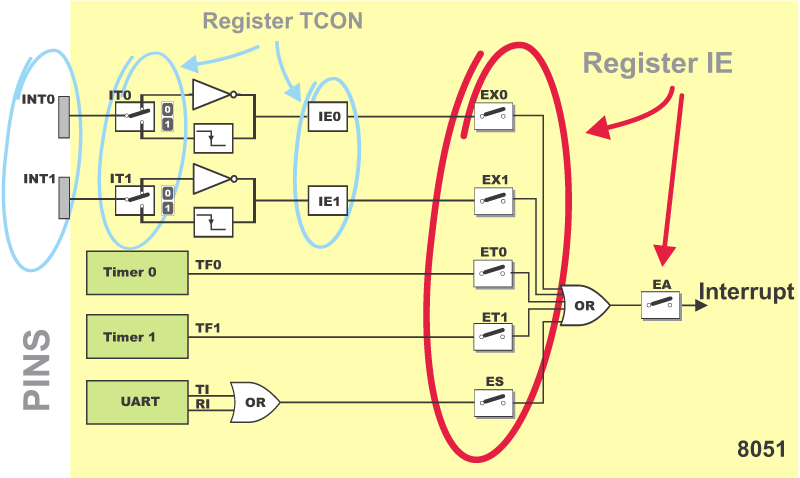
\includegraphics{/home/milav/Codes/MPMC/assets/imgs/181001_MCU_Question_Bank_Solved_html_969012cb171d85ed.png}
\caption{}
\end{figure}

\textbf{Interrupt Process}

\begin{enumerate}
\def\labelenumi{\arabic{enumi}.}
\item
  \textbf{Trigger:} An interrupt source (external pin, timer overflow,
  etc.) is triggered.
\item
  \textbf{Completion of Current Instruction:} The 8051 completes
  executing its current instruction.
\item
  \textbf{Saving State:} The microcontroller automatically pushes the
  current Program Counter (PC) onto the stack.
\item
  \textbf{Jump to ISR:} The 8051 jumps to the pre-determined memory
  address of the corresponding Interrupt Service Routine (ISR).
\item
  \textbf{ISR Execution:} The ISR code executes, handling the event that
  triggered the interrupt.
\item
  \textbf{Returning:} After the ISR completes, a 'RETI' instruction pops
  the PC value from the stack, resuming the original program flow.
\end{enumerate}

\textbf{Interrupt Control Registers}

\begin{itemize}
\item
  \textbf{IE (Interrupt Enable):} Enables or disables specific
  interrupts globally and individually within the system.
\item
  \textbf{IP (Interrupt Priority):} Assigns priority levels to each
  interrupt source. If multiple interrupts occur simultaneously, the one
  with higher priority is serviced first.
\end{itemize}

\textbf{Interrupt Vector Table}

\begin{longtable}[]{@{}lll@{}}
\toprule
Interrupt & Flag & Interrupt Vector Address \\
\midrule
\endhead
Reset & - & 0000H \\
INT0 & IE0 & 0003H \\
Timer 0 & TF0 & 000BH \\
INT1 & IE1 & 0013H \\
Timer 1 & TF1 & 001BH \\
Serial & TI/RI & 0023H \\
\bottomrule
\end{longtable}

\textbf{Key Points}

\begin{itemize}
\item
  \textbf{Priority:} The 8051 has a fixed interrupt priority structure
  (e.g., INT0 has the highest priority).
\item
  \textbf{Masking:} Interrupts can be turned on or off selectively using
  the IE register.
\item
  \textbf{Nesting:} Interrupts can potentially interrupt other
  interrupts, depending on their priority.
\item
  \textbf{Enabling Interrupts:} Interrupts must be enabled individually
  (e.g., IE0, ET0) and globally (EA = 1 in the IE register).
\end{itemize}

\begin{itemize}
\item
  \textbf{Interrupt Service Routines (ISRs):} ISRs contain the code to
  handle specific interrupt events. The microcontroller automatically
  jumps to the corresponding ISR's address in the vector table when an
  enabled interrupt occurs.
\end{itemize}

\hypertarget{381-ie-register}{%
\subsubsection{3.8.1. IE Register}\label{381-ie-register}}

\textbf{What is the IE Register?}

\begin{itemize}
\item
  The IE (Interrupt Enable) register is an 8-bit, bit-addressable
  Special Function Register (SFR) within 8051 microcontrollers.
\item
  Each bit in this register controls the enabling or disabling of
  specific interrupts within the system.
\end{itemize}

\textbf{IE Register Structure (Address: 0A8H, Byte addressable):}

\begin{longtable}[]{@{}llllllll@{}}
\toprule
IE.7 & IE.6 & IE.5 & IE.4 & IE.3 & IE.2 & IE.1 & IE.0 \\
\midrule
\endhead
EA & - & - & ES & ET1 & EX1 & ET0 & EX0 \\
\bottomrule
\end{longtable}

Here's the breakdown of the IE Register's bit functionality:

\begin{itemize}
\item
  \textbf{EA (Enable All):}

  \begin{itemize}
  \item
    '1' = Enables all interrupt sources (if their individual bits are
    also set to '1').
  \item
    '0' = Disables all interrupts, regardless of other bit settings.
  \end{itemize}
\item
  \textbf{Unused (3 bits):} These bits are typically reserved and have
  no assigned functionality.
\item
  \textbf{ES (Enable Serial Interrupt):}

  \begin{itemize}
  \item
    '1' = Enables serial port interrupt.
  \item
    '0' = Disables serial port interrupt.
  \end{itemize}
\item
  \textbf{ET1 (Enable Timer 1 Interrupt):}

  \begin{itemize}
  \item
    '1' = Enables the interrupt generated by Timer 1 overflow.
  \item
    '0' = Disables the Timer 1 interrupt.
  \end{itemize}
\item
  \textbf{EX1 (Enable External Interrupt 1):}

  \begin{itemize}
  \item
    '1' = Enables the external interrupt 1.
  \item
    '0' = Disables the external interrupt 1.
  \end{itemize}
\item
  \textbf{ET0 (Enable Timer 0 Interrupt):}

  \begin{itemize}
  \item
    '1' = Enables the interrupt generated by Timer 0 overflow.
  \item
    '0' = Disables the Timer 0 interrupt.
  \end{itemize}
\item
  \textbf{EX0 (Enable External Interrupt 0):}

  \begin{itemize}
  \item
    '1' = Enables the external interrupt 0.
  \item
    '0' = Disables the external interrupt 0.
  \end{itemize}
\end{itemize}

\begin{longtable}[]{@{}ll@{}}
\toprule
Bit & Function \\
\midrule
\endhead
EA & Global interrupt enable/disable Bit \\
ES & Enable Serial Interrupt Bit \\
ET1 & Enable Timer1 Interrupt Bit \\
EX1 & Enable External Interrupt 1 Bit \\
ET0 & Enable Timer0 Interrupt Bit \\
EX0 & Enable External Interrupt 1 Bit \\
\bottomrule
\end{longtable}

\textbf{How Interrupts Work with IE}

\begin{enumerate}
\def\labelenumi{\arabic{enumi}.}
\item
  \textbf{Global Enable:} The EA bit in the IE register must be set to
  '1' for any interrupt to function.
\item
  \textbf{Individual Enable:} Even if EA is set to '1', a specific
  interrupt request will be recognized only if the corresponding bit in
  the IE register is also set to '1'.
\end{enumerate}

\textbf{Examples}

\begin{enumerate}
\def\labelenumi{\arabic{enumi}.}
\item
  \textbf{Enabling All Interrupts}

\begin{Shaded}
\begin{Highlighting}[]
\NormalTok{IE = 0xFF;  // Set all bits in IE to \textquotesingle{}1\textquotesingle{}}
\end{Highlighting}
\end{Shaded}
\item
  \textbf{Enabling Only Timer 0 and External Interrupt 1}

\begin{Shaded}
\begin{Highlighting}[]
\NormalTok{IE = 0x89;  // Sets the ET0 and EX1 bits, the rest are \textquotesingle{}0\textquotesingle{}}
\end{Highlighting}
\end{Shaded}
\end{enumerate}

\textbf{Important Note:}

\begin{itemize}
\item
  Interrupts must also be configured in other registers for them to be
  active. For example:

  \begin{itemize}
  \item
    Timer interrupts require the timers to be started (TRx = '1' in
    TCON).
  \item
    External interrupts may need edge or level triggering configured
    (ITx bits in TCON).
  \end{itemize}
\item
  The 8051 has a priority system for multiple simultaneous interrupts.
  You can control the priority using the IP (Interrupt Priority)
  register.
\end{itemize}

\hypertarget{382-ip-register}{%
\subsubsection{3.8.2. IP Register}\label{382-ip-register}}

\textbf{What is the IP Register?}

\begin{itemize}
\item
  The IP (Interrupt Priority) register is an 8-bit, bit-addressable
  Special Function Register (SFR) used to manage the priority of
  interrupt sources in 8051 microcontrollers.
\item
  When multiple interrupts occur simultaneously, the IP register helps
  the system determine which interrupt to handle first.
\end{itemize}

\textbf{IP Register Structure (Address: 0B8H, Byte addressable)}

\begin{longtable}[]{@{}llllllll@{}}
\toprule
IP.7 & IP.6 & IP.5 & IP.4 & IP.3 & IP.2 & IP.1 & IP.0 \\
\midrule
\endhead
- & - & - & PS & PT1 & PX1 & PT0 & PX0 \\
\bottomrule
\end{longtable}

Each bit in the IP register is assigned a specific interrupt source,
providing two levels of priority (high or low):

\begin{itemize}
\item
  \textbf{Unused (3 bits):} These bits are typically reserved and have
  no assigned functionality.
\item
  \textbf{PS (Serial Interrupt Priority):}

  \begin{itemize}
  \item
    '1' = High priority.
  \item
    '0' = Low priority.
  \end{itemize}
\item
  \textbf{PT1 (Timer 1 Interrupt Priority):}

  \begin{itemize}
  \item
    '1' = High priority.
  \item
    '0' = Low priority.
  \end{itemize}
\item
  \textbf{PX1 (External Interrupt 1 Priority):}

  \begin{itemize}
  \item
    '1' = High priority.
  \item
    '0' = Low priority.
  \end{itemize}
\item
  \textbf{PT0 (Timer 0 Interrupt Priority):}

  \begin{itemize}
  \item
    '1' = High priority.
  \item
    '0' = Low priority.
  \end{itemize}
\item
  \textbf{PX0 (External Interrupt 0 Priority):}

  \begin{itemize}
  \item
    '1' = High priority.
  \item
    '0' = Low priority.
  \end{itemize}
\end{itemize}

\begin{longtable}[]{@{}ll@{}}
\toprule
Bit & Function \\
\midrule
\endhead
PS & Serial Interrupt Priority Bit \\
PT1 & Timer1 Interrupt Priority Bit \\
PX1 & External Interrupt 1 Priority Bit \\
PT0 & Timer0 Interrupt Priority Bit \\
PX0 & External Interrupt 0 Priority Bit \\
\bottomrule
\end{longtable}

\textbf{Default Interrupt Priority}

\begin{longtable}[]{@{}lll@{}}
\toprule
\textbf{Priority} & \textbf{Interrupt source} & \textbf{Intr. bit /
flag} \\
\midrule
\endhead
1 & External Interrupt 0 & INT0 \\
2 & Timer Interrupt 0 & TF0 \\
3 & External Interrupt 1 & INT1 \\
4 & Timer Interrupt 1 & TF1 \\
5 & Serial interrupt & (TI/RI) \\
\bottomrule
\end{longtable}

\textbf{How Interrupt Priorities Work with IP}

\begin{enumerate}
\def\labelenumi{\arabic{enumi}.}
\item
  \textbf{Interrupt Occurrence:} When one or more interrupts occur, the
  8051 checks the corresponding bits in the IP register.
\item
  \textbf{Priority Handling}

  \begin{itemize}
  \item
    Higher priority interrupts always take precedence over lower
    priority interrupts.
  \item
    If multiple interrupts of the same priority level occur, then the
    8051 uses a predefined internal polling sequence to determine the
    order for servicing the interrupts.
  \end{itemize}
\end{enumerate}

\textbf{Examples}

\begin{enumerate}
\def\labelenumi{\arabic{enumi}.}
\item
  \textbf{Configuring Timer 0 as Highest Priority, External Interrupt 1
  as Lowest}

\begin{Shaded}
\begin{Highlighting}[]
\NormalTok{IP = 0x12; // Sets PT0 to \textquotesingle{}1\textquotesingle{} (high), PX1 to \textquotesingle{}0\textquotesingle{} (low), others remain \textquotesingle{}0\textquotesingle{}}
\end{Highlighting}
\end{Shaded}
\item
  \textbf{Setting All Interrupts to Low Priority}

\begin{Shaded}
\begin{Highlighting}[]
\NormalTok{IP = 0x00; // All bits set to \textquotesingle{}0\textquotesingle{} for low priority}
\end{Highlighting}
\end{Shaded}
\end{enumerate}

\textbf{Important Notes:}

\begin{itemize}
\item
  The IP register only determines the priority among simultaneously
  occurring interrupts. The interrupt itself still needs to be enabled
  globally (EA bit in the IE register) and individually (Ex and ETx bits
  in the IE register).
\item
  The priority structure and internal polling sequence for the 8051
  microcontroller can be found in your specific microcontroller's
  datasheet.
\end{itemize}

\textbf{Default Interrupt Priority}

\begin{longtable}[]{@{}lll@{}}
\toprule
\textbf{Priority} & \textbf{Interrupt source} & \textbf{Intr. bit /
flag} \\
\midrule
\endhead
1 & External Interrupt 0 & INT0 \\
2 & Timer Interrupt 0 & TF0 \\
3 & External Interrupt 1 & INT1 \\
4 & Timer Interrupt 1 & TF1 \\
5 & Serial interrupt & (TI/RI) \\
\bottomrule
\end{longtable}

\hypertarget{4-unit-iv-8051-programming}{%
\section{4. Unit IV: 8051
Programming}\label{4-unit-iv-8051-programming}}

\hypertarget{41-addressing-modes}{%
\subsection{4.1. Addressing Modes}\label{41-addressing-modes}}

\textbf{What is an Addressing Mode?}

An Addressing Mode is a way to locate a target Data, which is also
called as Operand. The 8051 Family of Microcontrollers allows five types
of Addressing Modes for addressing the Operands. They are:

\begin{itemize}
\item
  Register Addressing
\item
  Direct Addressing
\item
  Indirect Addressing
\item
  Immediate Addressing
\item
  Indexed(Base Relative Addressing with DPTR) Addressing
\item
  Relative Addressing
\item
  Bit Addressing
\end{itemize}

\textbf{Key Addressing Modes in the 8051}

\begin{enumerate}
\def\labelenumi{\arabic{enumi}.}
\item
  \textbf{Register Addressing}

  \begin{itemize}
  \item
    \textbf{How it Works:} The operand of the instruction directly
    specifies one of the 8051's registers (A, B, R0-R7).
  \item
    \textbf{Example:} \texttt{MOV\ A,\ R2} (Copy the contents of R2 into
    the accumulator)
  \item
    \textbf{Fast and Efficient:} No additional memory accesses are
    needed.
  \end{itemize}
\item
  \textbf{Direct Addressing}

  \begin{itemize}
  \item
    \textbf{How it Works:} The instruction contains an 8-bit address
    that directly points to a location in the internal RAM or Special
    Function Registers (SFRs).
  \item
    \textbf{Example:} \texttt{MOV\ 45H,\ A} (Store the value in the
    accumulator into internal RAM location 45H)
  \item
    \textbf{Accesses only first 256 bytes:} Limited to accessing the
    lower portion of internal RAM and SFRs.
  \end{itemize}
\item
  \textbf{Indirect Addressing}

  \begin{itemize}
  \item
    \textbf{How it Works:} The instruction specifies a register (R0 or
    R1) that holds the memory address of where the data actually
    resides.
  \item
    \textbf{Example:} \texttt{MOV\ A,\ @R0} (Copy the byte pointed to by
    the address in R0 into the accumulator).
  \item
    \textbf{Flexibility:} Allows dynamic calculation of data locations.
  \end{itemize}
\item
  \textbf{Immediate Addressing}

  \begin{itemize}
  \item
    \textbf{How it Works:} The data to be used is embedded directly
    within the instruction itself. Preceded by the '\#' symbol.
  \item
    \textbf{Example:} \texttt{MOV\ A,\ \#60H} (Load the value 60H into
    the accumulator).
  \item
    \textbf{Convenient for constants:} Useful for loading fixed values.
  \end{itemize}
\item
  \textbf{Indexed(Base Relative Addressing with DPTR)}

  \begin{itemize}
  \item
    \textbf{How it Works}: Used for accessing external RAM. The Data
    Pointer (DPTR) provides a 16-bit base address, and an 8-bit offset
    within the instruction specifies a location relative to that base.
  \item
    \textbf{Example}: \texttt{MOVX\ A,\ @DPTR} (Copy byte from external
    RAM pointed to by DPTR into the accumulator)
  \item
    \textbf{Expanded Memory:} Access up to 64KB of external memory
  \end{itemize}
\item
  \textbf{Relative Addressing}

  \begin{itemize}
  \item
    \textbf{How it Works:} The instruction provides an offset that's
    relative to the Program Counter (PC). This offset (usually a signed
    8-bit value) is added to the address of the \emph{next} instruction
    to determine the target address for a jump or branch.
  \item
    \textbf{Example:} JRNE 20H (Jump if Zero flag is not set, relative
    to an address 20H bytes away from the next instruction).
  \item
    \textbf{Advantages:}

    \begin{itemize}
    \item
      \textbf{Position-independent code:} Allows relocatable code blocks
      as the jump target is calculated relative to the current position.
    \item
      \textbf{Compact encoding:} Typically uses a smaller offset within
      the instruction, saving program memory space.
    \end{itemize}
  \end{itemize}
\item
  \textbf{Bit Addressing}

  \begin{itemize}
  \item
    \textbf{How it Works:} Instructions directly address individual bits
    within three areas:

    \begin{enumerate}
    \def\labelenumii{\arabic{enumii}.}
    \item
      \textbf{Internal RAM (bit-addressable area):} Certain bytes of
      internal RAM have bits that can be addressed individually.
    \item
      \textbf{Special Function Registers (SFRs):} Many control and
      status bits within SFRs can be directly manipulated.
    \item
      \textbf{I/O Ports (sometimes):} Certain I/O devices have bit-level
      control.
    \end{enumerate}
  \item
    \textbf{Example:} SETB 20H (Set the bit at location 20H within the
    bit-addressable area of internal RAM).
  \item
    \textbf{Advantages:}

    \begin{itemize}
    \item
      \textbf{Fine-grained control:} Allows modification or checking of
      single bits within registers or memory locations.
    \item
      \textbf{Efficient for flags and control bits:} Avoids the need to
      manipulate entire bytes when dealing with single-bit flags.
    \end{itemize}
  \end{itemize}
\end{enumerate}

\hypertarget{411-immediate-addressing-mode}{%
\subsubsection{4.1.1. Immediate addressing
mode}\label{411-immediate-addressing-mode}}

\textbf{Immediate Addressing Mode: What is it?}

\begin{itemize}
\item
  In immediate addressing mode, the data (or value) to be operated on is
  directly included within the instruction itself.
\item
  The symbol "\#" usually indicates that the value following it is
  immediate data.
\end{itemize}

\textbf{Key Advantages}

\begin{itemize}
\item
  \textbf{Speed:} Immediate addressing is fast because the data is
  immediately available to the processor; no additional memory fetching
  is needed.
\item
  \textbf{Simplicity:} This is a simple addressing mode, great for using
  fixed constants within your code.
\end{itemize}

\textbf{Examples}

Here are some examples of 8051 instructions using immediate addressing
mode:

\begin{enumerate}
\def\labelenumi{\arabic{enumi}.}
\item
  \textbf{Loading a value into the accumulator:}

\begin{Shaded}
\begin{Highlighting}[]
\NormalTok{MOV A, \#50H  ; Load the value 50 (hexadecimal) into the accumulator (register A)}
\end{Highlighting}
\end{Shaded}
\item
  \textbf{Adding an immediate value to a register:}

\begin{Shaded}
\begin{Highlighting}[]
\NormalTok{ADD R2, \#10  ; Add the value 10 to register R2}
\end{Highlighting}
\end{Shaded}
\item
  \textbf{Moving data using the Data Pointer (DPTR):}

\begin{Shaded}
\begin{Highlighting}[]
\NormalTok{MOV DPTR, \#2500H ; Load the immediate value 2500H into the Data Pointer,}
\NormalTok{                  ; pointing to an external memory location}
\end{Highlighting}
\end{Shaded}
\end{enumerate}

\textbf{Important Note:} In the 8051, immediate data is generally
limited to 8-bits (0-255 or 00H to FFH).

\textbf{When to Use Immediate Addressing Mode}

Immediate addressing is ideal in the following situations:

\begin{itemize}
\item
  \textbf{Working with constants:} When you know the exact value at the
  time of writing the code.
\item
  \textbf{Initializing variables:} Setting initial values for variables
  at the start of your program.
\item
  \textbf{Performing simple calculations:} When you need to add or
  subtract small, fixed values.
\end{itemize}

\hypertarget{412-register-addressing-mode}{%
\subsubsection{4.1.2. Register addressing
mode}\label{412-register-addressing-mode}}

\textbf{Register Addressing Mode: The Basics}

\begin{itemize}
\item
  In this mode, the operands (the data the instruction works with) are
  stored within the 8051's internal registers.
\item
  The 8051 has a set of general-purpose registers named R0 through R7,
  along with the accumulator (A).
\end{itemize}

\textbf{Why Use It}

\begin{itemize}
\item
  \textbf{Speed:} Register addressing is the fastest addressing mode
  since data is accessed directly from the CPU's internal registers. No
  time is spent fetching data from external memory.
\item
  \textbf{Efficiency:} It uses fewer instruction bytes, making your code
  more compact.
\end{itemize}

\textbf{Example Instructions}

Let's see register addressing in action:

\begin{enumerate}
\def\labelenumi{\arabic{enumi}.}
\item
  \textbf{Moving data between registers:}

\begin{Shaded}
\begin{Highlighting}[]
\NormalTok{MOV R5, R1  ; Move the contents of register R1 into register R5}
\end{Highlighting}
\end{Shaded}
\item
  \textbf{Adding the contents of two registers:}

\begin{Shaded}
\begin{Highlighting}[]
\NormalTok{ADD A, R6   ; Add the contents of register R6 to the accumulator (A) and store the result in the accumulator}
\end{Highlighting}
\end{Shaded}
\item
  \textbf{Clearing a register:}

\begin{Shaded}
\begin{Highlighting}[]
\NormalTok{CLR R0      ; Clear register R0 (set its value to 0)}
\end{Highlighting}
\end{Shaded}
\end{enumerate}

\textbf{Key Points}

\begin{itemize}
\item
  Register addressing mode is heavily used in 8051 programs because of
  its speed and efficiency.
\item
  You can't directly move data between two registers that aren't the
  Accumulator (A). You'll often see instructions temporarily using the
  accumulator to facilitate data transfers between registers.
\end{itemize}

\hypertarget{413-direct-addressing-mode}{%
\subsubsection{4.1.3. Direct addressing
mode}\label{413-direct-addressing-mode}}

\textbf{Direct Addressing Mode: Core Concept}

\begin{itemize}
\item
  In direct addressing mode, the instruction contains the direct 8-bit
  address of the data within the 8051's internal RAM or Special Function
  Registers (SFRs).
\end{itemize}

\textbf{Restrictions}

\begin{itemize}
\item
  \textbf{Address Space:} Direct addressing can only access the
  following:

  \begin{itemize}
  \item
    Internal RAM locations from 00H to 7FH.
  \item
    Special Function Registers (SFRs) from 80H to FFH.
  \end{itemize}
\end{itemize}

\textbf{Advantages}

\begin{itemize}
\item
  \textbf{Reasonable speed:} It's slower than register addressing, but
  still relatively fast since you're accessing the internal memory.
\item
  \textbf{Variable data:} Useful when working with variables whose
  location in memory might change.
\end{itemize}

\textbf{Examples}

\begin{enumerate}
\def\labelenumi{\arabic{enumi}.}
\item
  \textbf{Loading data from Internal RAM:}

\begin{Shaded}
\begin{Highlighting}[]
\NormalTok{MOV A, 35H  ; Load the contents of internal RAM location 35H into the accumulator (A)}
\end{Highlighting}
\end{Shaded}
\item
  \textbf{Storing data in Internal RAM:}

\begin{Shaded}
\begin{Highlighting}[]
\NormalTok{MOV 50H, A  ; Store the contents of the accumulator (A) into internal RAM location 50H}
\end{Highlighting}
\end{Shaded}
\item
  \textbf{Controlling an output port:}

\begin{Shaded}
\begin{Highlighting}[]
\NormalTok{MOV P1, \#90H ; Send the value 90H (hexadecimal) to port 1 (SFR address 90H)}
\end{Highlighting}
\end{Shaded}
\end{enumerate}

\textbf{Important Notes}

\begin{itemize}
\item
  Direct addressing mode does \textbf{not} use the "\#" symbol to
  differentiate between immediate data and addresses.
\item
  SFRs (Special Function Registers) control the 8051's hardware
  peripherals and are accessed using direct addressing.
\end{itemize}

\hypertarget{414-indirect-addressing-mode}{%
\subsubsection{4.1.4. Indirect addressing
mode}\label{414-indirect-addressing-mode}}

\textbf{Indirect Addressing Mode: The Basics}

\begin{itemize}
\item
  In indirect addressing mode, the instruction doesn't contain the
  actual data address. Instead, it holds the address of a register that
  points to where the data is located in memory.
\item
  The "@" symbol precedes the register name to indicate indirect
  addressing.
\item
  Indirect addressing supports two register pairs in the 8051:

  \begin{itemize}
  \item
    \textbf{R0 and R1:} For accessing internal RAM
  \item
    \textbf{DPTR (Data Pointer):} For accessing internal RAM and
    external RAM (if present)
  \end{itemize}
\end{itemize}

\textbf{Why Use It}

\begin{itemize}
\item
  \textbf{Flexibility:} This is the key advantage. It allows you to
  calculate or dynamically change the memory location to be accessed
  during program execution.
\item
  \textbf{Data Structures:} Perfect for arrays, tables, and other data
  structures where you need to access data elements sequentially.
\end{itemize}

\textbf{Examples}

\begin{enumerate}
\def\labelenumi{\arabic{enumi}.}
\item
  \textbf{Accessing internal RAM using R0:}

\begin{Shaded}
\begin{Highlighting}[]
\NormalTok{MOV R0, \#40H  ; Load the value 40H into register R0}
\NormalTok{MOV A, @R0    ; Load the contents of the internal RAM location pointed to by R0 (which is 40H) into the accumulator}
\end{Highlighting}
\end{Shaded}
\item
  \textbf{Accessing external RAM using DPTR:}

\begin{Shaded}
\begin{Highlighting}[]
\NormalTok{MOV DPTR, \#3000H  ; Load the value 3000H into the Data Pointer}
\NormalTok{MOVX A, @DPTR     ; Load the contents of external RAM location 3000H into the accumulator}
\NormalTok{                      ; (note the use of MOVX for external memory)}
\end{Highlighting}
\end{Shaded}
\item
  \textbf{Table Lookup:}

\begin{Shaded}
\begin{Highlighting}[]
\NormalTok{MOV R0, \#TABLE\_START  ; Load the starting address of a table into R0}
\NormalTok{MOV A, @R0            ; Load the first element of the table into the accumulator}
\NormalTok{INC R0                ; Increment R0 to point to the next element}
\NormalTok{; ... repeat as needed}
\end{Highlighting}
\end{Shaded}
\end{enumerate}

\textbf{Key Points}

\begin{itemize}
\item
  Indirect addressing gives you much more flexibility for accessing data
  in different memory locations.
\item
  Using 'MOVX' is necessary for accessing external memory with indirect
  addressing.
\end{itemize}

\hypertarget{415-indexed-addressing-mode}{%
\subsubsection{4.1.5. Indexed addressing
mode}\label{415-indexed-addressing-mode}}

\textbf{Indexed Addressing Mode: Combining Base + Offset}

\begin{itemize}
\item
  Indexed addressing mode provides a way to access data in the Program
  Memory (code memory) of the 8051.
\item
  It combines the contents of a base register (either the Data Pointer -
  DPTR -- or the Program Counter - PC) with the contents of the
  Accumulator (A) to form the effective address of the data you want to
  access.
\end{itemize}

\textbf{Why use it?}

\begin{itemize}
\item
  \textbf{Accessing data tables in program memory:} Ideal for working
  with tables or arrays of data stored in the code space of the 8051.
\end{itemize}

\textbf{Key Points}

\begin{itemize}
\item
  The instruction "MOVC" is used for indexed addressing in the 8051. The
  'C' indicates that the instruction is accessing Code memory.
\end{itemize}

\textbf{Examples}

\begin{enumerate}
\def\labelenumi{\arabic{enumi}.}
\item
  \textbf{Using the Data Pointer (DPTR):}

\begin{Shaded}
\begin{Highlighting}[]
\NormalTok{MOV DPTR, \#MY\_TABLE   ; Load the starting address of \textquotesingle{}MY\_TABLE\textquotesingle{} into DPTR}
\NormalTok{MOV A, \#03H           ; Load index \textquotesingle{}3\textquotesingle{} into accumulator}
\NormalTok{MOVC A, @A+DPTR       ; Fetch the data at the address (DPTR value + 3)}
\NormalTok{                          ; from program memory and load it into the accumulator}
\end{Highlighting}
\end{Shaded}
\item
  \textbf{Using the Program Counter (PC):}

\begin{Shaded}
\begin{Highlighting}[]
\NormalTok{MOV A, \#05H           ; Load index \textquotesingle{}5\textquotesingle{} into accumulator}
\NormalTok{MOVC A, @A+PC         ; Fetch the data at the address (PC value + 5)}
\NormalTok{                          ; from program memory and load it into the accumulator}
\end{Highlighting}
\end{Shaded}
\end{enumerate}

\textbf{Explanation of Example 1}

\begin{itemize}
\item
  Let's say 'MY\_TABLE' starts at program memory address 2000H.
\item
  With the index (offset) of 3 in the accumulator, the instruction
  \texttt{MOVC\ A,\ @A+DPTR} will access the data stored at address
  2003H in program memory.
\end{itemize}

\textbf{Important Notes}

\begin{itemize}
\item
  Indexed addressing is limited to accessing data within the program
  memory of the 8051 microcontroller.
\item
  It cannot be used to modify the program memory itself (ROM is
  read-only).
\end{itemize}

\hypertarget{416-relative-addressing-mode}{%
\subsubsection{4.1.6. Relative addressing
mode}\label{416-relative-addressing-mode}}

\textbf{Relative Addressing Mode: Jumping by Offset}

\begin{itemize}
\item
  In relative addressing mode, the instruction contains an 8-bit signed
  offset (a value that can be positive or negative). This offset is
  added to the Program Counter (PC) to determine the address of the next
  instruction to be executed.
\item
  Primarily used for conditional jumps and branching within your code.
\end{itemize}

\textbf{Why Use It?}

\begin{itemize}
\item
  \textbf{Code Relocatability:} Code using relative addressing becomes
  position-independent. This means you can move the code block to a
  different memory location without modifying branch instructions.
\item
  \textbf{Conditional Branching:} Ideal for instructions like
  \texttt{SJMP} (Short Jump), \texttt{JZ} (Jump if Zero), etc.
\end{itemize}

\textbf{Example}

\begin{Shaded}
\begin{Highlighting}[]
\NormalTok{HERE:   MOV A, R0   ; Some instructions...}
\NormalTok{        JZ  TARGET  ; Jump to \textquotesingle{}TARGET\textquotesingle{} if the accumulator is zero}
\NormalTok{        ...         ; More instructions...}
\NormalTok{TARGET: INC R5      ; Target location if the jump was taken}
\end{Highlighting}
\end{Shaded}

\textbf{Explanation}

\begin{itemize}
\item
  Let's say the instruction \texttt{JZ\ TARGET} is at memory location
  1000H.
\item
  The assembler figures out the offset needed to reach \texttt{TARGET}
  from the current location and includes it as a second byte in the
  instruction.
\item
  If \texttt{TARGET} is 10 bytes ahead, the offset will be +10. If
  \texttt{TARGET} is 5 bytes behind, the offset will be -5.
\item
  The range of a relative jump is limited to -128 to +127 bytes from the
  current instruction.
\end{itemize}

\textbf{Key Points}

\begin{itemize}
\item
  Relative addressing makes your code more compact, as you don't need
  full target addresses within the jump instructions.
\item
  Watch out for jump range limits! It can only jump a limited distance
  forward or backward.
\end{itemize}

\hypertarget{417-bit-addressing-mode}{%
\subsubsection{4.1.7. Bit addressing
mode}\label{417-bit-addressing-mode}}

\textbf{Bit Addressing Mode: Manipulating Individual Bits}

\begin{itemize}
\item
  Bit addressing mode provides fine-grained control by allowing you to
  directly address and manipulate individual bits within:

  \begin{itemize}
  \item
    \textbf{Internal RAM (bit-addressable area):} Locations 20H to 2FH
  \item
    \textbf{Special Function Registers (SFRs): } Many SFRs have
    individual bits that control specific hardware functions.
  \end{itemize}
\end{itemize}

\textbf{Key Points}

\begin{itemize}
\item
  Bit addresses range from 00H to 7FH.
\item
  Bit addressing uses a direct addressing approach, where the
  instruction includes the full bit address.
\end{itemize}

\textbf{Instructions for Bit Addressing}

\begin{itemize}
\item
  \textbf{SETB:} Sets a specified bit to 1.
\item
  \textbf{CLR:} Clears a specified bit to 0.
\item
  \textbf{CPL:} Complements a specified bit (changes 0 to 1, or 1 to 0).
\end{itemize}

\textbf{Examples}

\begin{enumerate}
\def\labelenumi{\arabic{enumi}.}
\item
  \textbf{Controlling a bit in the P1 SFR (Port 1):}

\begin{Shaded}
\begin{Highlighting}[]
\NormalTok{SETB P1.0  ; Set bit 0 of Port 1 (making output pin P1.0 go high)}
\NormalTok{CLR P1.5   ; Clear bit 5 of Port 1 (making output pin P1.5 go low)}
\end{Highlighting}
\end{Shaded}
\item
  \textbf{Checking the status of a flag bit in the TCON SFR:}

\begin{Shaded}
\begin{Highlighting}[]
\NormalTok{JB TF0, OVERFLOW\_ROUTINE  ; Jump to \textquotesingle{}OVERFLOW\_ROUTINE\textquotesingle{} if the Timer 0 overflow flag (TF0) in the TCON register is set.}
\end{Highlighting}
\end{Shaded}
\end{enumerate}

\textbf{Why Use Bit Addressing}

\begin{itemize}
\item
  \textbf{Direct Hardware Control:} Modifying specific bits in SFRs
  allows you to configure and control various hardware peripherals of
  the 8051 microcontroller.
\item
  \textbf{Efficient use of RAM:} You can pack multiple flags or status
  indicators into a single byte of internal RAM.
\end{itemize}

\textbf{Important Notes}

\begin{itemize}
\item
  Not all SFRs are bit-addressable. You'll need to consult the 8051
  datasheet for details.
\item
  Remember, bit addresses are different from regular byte addresses.
\end{itemize}

\hypertarget{42-8051-instruction-set}{%
\subsection{4.2. 8051 Instruction Set}\label{42-8051-instruction-set}}

\begin{itemize}
\item
  The 8051 has a variable-length instruction set. Instructions range
  from 1 to 3 bytes long.
\item
  There are 111 core instructions in the 8051.
\item
  These instructions are broadly classified into the following groups:
\end{itemize}

\textbf{1. Data Transfer Instructions}

\begin{itemize}
\item
  \textbf{Moving data between registers:} MOV, XCH, XCHD
\item
  \textbf{Moving data between internal RAM and registers:} MOV
\item
  \textbf{Moving data to/from external RAM (if present):} MOVX
\item
  \textbf{Stack operations:} PUSH, POP
\item
  \textbf{Loading immediate values:} MOV
\item
  \textbf{Absolute and relative jumps:} LJMP, SJMP
\item
  \textbf{Conditional jumps:} JZ, JNZ, JC, JBC, etc.
\item
  \textbf{Subroutine calls and returns:} ACALL, LCALL, RET, RETI
\end{itemize}

\textbf{2. Arithmetic Instructions}

\begin{itemize}
\item
  \textbf{Addition:} ADD, ADDC (add with carry)
\item
  \textbf{Subtraction:} SUBB (subtract with borrow)
\item
  \textbf{Increment/Decrement:} INC, DEC
\item
  \textbf{Multiplication:} MUL
\item
  \textbf{Division:} DIV
\item
  \textbf{Comparison:} CJNE
\end{itemize}

\textbf{3. Logical Instructions}

\begin{itemize}
\item
  \textbf{AND:} ANL
\item
  \textbf{OR:} ORL
\item
  \textbf{XOR:} XRL
\end{itemize}

\textbf{4. Program Branching Instructions}

\begin{itemize}
\item
  \textbf{Unconditional jumps:} LJMP, SJMP
\item
  \textbf{Conditional jumps based on flags and accumulator status:} JZ
  (Jump if Zero), JNZ (Jump if Not Zero), JC (Jump if Carry), etc.
\item
  \textbf{Conditional jumps based on single bits:} JB (Jump if Bit set),
  JNB (Jump if Bit Not set), JBC (Jump if Bit and Clear)
\item
  \textbf{Subroutine calls:} ACALL, LCALL
\item
  \textbf{Subroutine returns:} RET, RETI
\end{itemize}

\textbf{5. Boolean or Bit Manipulation Instructions}

\begin{itemize}
\item
  \textbf{Setting bits:} SETB
\item
  \textbf{Clearing bits:} CLR
\item
  \textbf{Complementing (inverting) bits:} CPL
\item
  \textbf{Logical operations on bits:} ANL, ORL, XRL,
\item
  \textbf{Conditional jumps based on individual bit states:} JB, JNB,
  JBC
\end{itemize}

The following nomenclatures for register, data, address and variables
are used while write instructions.

\begin{itemize}
\item
  A: Accumulator
\item
  B: "B" register
\item
  C: Carry bit
\item
  Rn: Register R0 - R7 of the currently selected register bank
\item
  Direct: 8-bit internal direct address for data. The data could be in
  lower 128bytes of RAM (00 - 7FH) or it could be in the special
  function register (80 - FFH).
\item
  @Ri: 8-bit external or internal RAM address available in register R0
  or R1. This is used for indirect addressing mode.
\item
  \#data8: Immediate 8-bit data available in the instruction.
\item
  \#data16: Immediate 16-bit data available in the instruction.
\item
  Addr11: 11-bit destination address for short absolute jump. Used by
  instructions AJMP \& ACALL. Jump range is 2 kbyte (one page).
\item
  Addr16: 16-bit destination address for long call or long jump.
\item
  Rel: 2's complement 8-bit offset (one - byte) used for short jump
  (SJMP) and all conditional jumps.
\item
  bit: Directly addressed bit in internal RAM or SFR
\end{itemize}

\hypertarget{421-data-transfer-instructions}{%
\subsubsection{4.2.1. Data Transfer
Instructions}\label{421-data-transfer-instructions}}

Data transfer instructions move the content of one register to another.
The register the content of which is moved remains unchanged. If they
have the suffix ``X'' (MOVX), the data is exchanged with external
memory.

These instructions move data between various registers, internal RAM,
external RAM, and I/O ports of the 8051. Here's a breakdown of the key
types:

\textbf{1. Register-to-Register Transfers}

\begin{itemize}
\item
  \textbf{MOV instruction:} The most versatile data transfer
  instruction.
\item
  \textbf{Examples:}

  \begin{itemize}
  \item
    \texttt{MOV\ A,\ R5} - Copies the contents of register R5 into the
    accumulator.
  \item
    \texttt{MOV\ R2,\ \#45H} - Loads the immediate value 45H into
    register R2.
  \item
    \texttt{MOV\ P1,\ A} - Copies the accumulator's contents to port P1
    (output).
  \end{itemize}
\end{itemize}

\textbf{2. Direct Addressing}

\begin{itemize}
\item
  \textbf{MOV instruction with 'direct' addressing mode:} Accesses
  internal RAM or Special Function Registers (SFRs).
\item
  \textbf{Examples:}

  \begin{itemize}
  \item
    \texttt{MOV\ 50H,\ A} - Stores the value in the accumulator to
    internal RAM location 50H.
  \item
    \texttt{MOV\ ACC,\ 55H} - Loads the byte from internal RAM location
    55H into the accumulator.
  \item
    \texttt{MOV\ TMOD,\ \#01H} - Sets Timer 0 into mode 1.
  \end{itemize}
\end{itemize}

\textbf{3. Indirect Addressing}

\begin{itemize}
\item
  \textbf{MOV instruction using registers as pointers:} The register
  holds the address of the data.
\item
  \textbf{Examples:}

  \begin{itemize}
  \item
    \texttt{MOV\ A,\ @R0} - Copies the byte pointed to by register R0
    into the accumulator.
  \item
    \texttt{MOV\ @R1,\ 33H} - Stores the value 33H at the address
    pointed to by R1.
  \end{itemize}
\end{itemize}

\textbf{4. External Memory Transfers}

\begin{itemize}
\item
  \textbf{MOVX instruction:} Used to access external RAM.
\item
  \textbf{Examples:}

  \begin{itemize}
  \item
    \texttt{MOVX\ A,\ @DPTR} -- Copies a byte from external RAM (address
    in DPTR) into the accumulator.
  \item
    \texttt{MOVX\ @DPTR,\ A} -- Copies the contents of the accumulator
    into external RAM (address in DPTR).
  \end{itemize}
\end{itemize}

\textbf{5. Special Data Transfers}

\begin{itemize}
\item
  \textbf{PUSH instruction:} Pushes data onto the stack (internal RAM).
\item
  \textbf{POP instruction:} Pops data off the stack.
\end{itemize}

\textbf{Example: Data Sorting Routine}

Consider a simple routine to sort three numbers stored at internal RAM
locations 40H, 41H, and 42H:

\begin{Shaded}
\begin{Highlighting}[]
\NormalTok{COMPARE: MOV A, 40H    ; Load the first number}
\NormalTok{         MOVC A, @A+DPTR ; Load the second number (assuming DPTR points to RAM)}
\NormalTok{         JC  SWAP        ; Jump to SWAP if the first is greater than the second}

\NormalTok{         MOV A, 41H     ; Load the second number}
\NormalTok{         MOVC A, @A+DPTR ; Load the third number}
\NormalTok{         JC  SWAP        ; Jump to SWAP if the second is greater than the third}
\NormalTok{         ; ... (rest of your code)}

\NormalTok{SWAP:    ; ... (Code to swap values)}
\end{Highlighting}
\end{Shaded}

\begin{longtable}[]{@{}llll@{}}
\toprule
\textbf{Mnemonic} & \textbf{Description} & \textbf{Byte} &
\textbf{Cycle} \\
\midrule
\endhead
MOV A,Rn & Moves the register to the accumulator & 1 & 1 \\
MOV A,direct & Moves the direct byte to the accumulator & 2 & 2 \\
MOV A,@Ri & Moves the indirect RAM to the accumulator & 1 & 2 \\
MOV A,\#data & Moves the immediate data to the accumulator & 2 & 2 \\
MOV Rn,A & Moves the accumulator to the register & 1 & 2 \\
MOV Rn,direct & Moves the direct byte to the register & 2 & 4 \\
MOV Rn,\#data & Moves the immediate data to the register & 2 & 2 \\
MOV direct,A & Moves the accumulator to the direct byte & 2 & 3 \\
MOV direct,Rn & Moves the register to the direct byte & 2 & 3 \\
MOV direct,direct & Moves the direct byte to the direct byte & 3 & 4 \\
MOV direct,@Ri & Moves the indirect RAM to the direct byte & 2 & 4 \\
MOV direct,\#data & Moves the immediate data to the direct byte & 3 &
3 \\
MOV @Ri,A & Moves the accumulator to the indirect RAM & 1 & 3 \\
MOV @Ri,direct & Moves the direct byte to the indirect RAM & 2 & 5 \\
MOV @Ri,\#data & Moves the immediate data to the indirect RAM & 2 & 3 \\
MOV DPTR,\#data & Moves a 16-bit data to the data pointer & 3 & 3 \\
MOVC A,@A+DPTR & Moves the code byte relative to the DPTR to the
accumulator (address=A+DPTR) & 1 & 3 \\
MOVC A,@A+PC & Moves the code byte relative to the PC to the accumulator
(address=A+PC) & 1 & 3 \\
MOVX A,@Ri & Moves the external RAM (8-bit address) to the accumulator &
1 & 3-10 \\
MOVX A,@DPTR & Moves the external RAM (16-bit address) to the
accumulator & 1 & 3-10 \\
MOVX @Ri,A & Moves the accumulator to the external RAM (8-bit address) &
1 & 4-11 \\
MOVX @DPTR,A & Moves the accumulator to the external RAM (16-bit
address) & 1 & 4-11 \\
PUSH direct & Pushes the direct byte onto the stack & 2 & 4 \\
POP direct & Pops the direct byte from the stack/td\textgreater{} & 2 &
3 \\
XCH A,Rn & Exchanges the register with the accumulator & 1 & 2 \\
XCH A,direct & Exchanges the direct byte with the accumulator & 2 & 3 \\
XCH A,@Ri & Exchanges the indirect RAM with the accumulator & 1 & 3 \\
XCHD A,@Ri & Exchanges the low-order nibble indirect RAM with the
accumulator & 1 & 3 \\
\bottomrule
\end{longtable}

\hypertarget{422-arithmetic-instructions}{%
\subsubsection{4.2.2. Arithmetic
Instructions}\label{422-arithmetic-instructions}}

Arithmetic instructions perform several basic operations such as
addition, subtraction, division, multiplication etc. After execution,
the result is stored in the first operand. For example: ADD A,R1 - The
result of addition (A+R1) will be stored in the accumulator.

\textbf{Core Arithmetic Instructions}

\begin{itemize}
\item
  \textbf{ADD (Addition):} Adds the value of a source operand to the
  accumulator (A).

  \begin{itemize}
  \item
    Example: \texttt{ADD\ A,\ R2} (Adds contents of register R2 to the
    accumulator)
  \end{itemize}
\item
  \textbf{ADDC (Addition with Carry):} Adds a source operand plus the
  previous carry flag (CF) to the accumulator (A)

  \begin{itemize}
  \item
    Example: \texttt{ADDC\ A,\ \#30H} (Adds 30H and the carry flag to
    the accumulator)
  \end{itemize}
\item
  \textbf{SUBB (Subtraction with Borrow):} Subtracts the value of a
  source operand and the carry flag (CF) from the accumulator (A).

  \begin{itemize}
  \item
    Example: \texttt{SUBB\ A,\ @R0} (Subtracts the value pointed to by
    R0 and the carry flag from the accumulator)
  \end{itemize}
\item
  \textbf{INC (Increment):} Increments the value of a register or direct
  memory location by 1.

  \begin{itemize}
  \item
    Example: \texttt{INC\ R5} (Increments the value of register R5)
  \end{itemize}
\item
  \textbf{DEC (Decrement):} Decrements the value of a register or direct
  memory location by 1.

  \begin{itemize}
  \item
    Example: \texttt{DEC\ 50H} (Decrements the value at internal RAM
    location 50H)
  \end{itemize}
\item
  \textbf{MUL (Multiplication):} Multiplies the accumulator (A) with
  register B. Result stored in both the accumulator and register B.

  \begin{itemize}
  \item
    Example: \texttt{MUL\ AB}
  \end{itemize}
\item
  \textbf{DIV (Division):} Divides the accumulator (A) by register B.
  Quotient is stored in the accumulator and the remainder in register B.

  \begin{itemize}
  \item
    Example: \texttt{DIV\ AB}
  \end{itemize}
\end{itemize}

\textbf{Important Notes}

\begin{itemize}
\item
  Arithmetic operations affect the following flags:

  \begin{itemize}
  \item
    C (Carry Flag)
  \item
    AC (Auxiliary Carry Flag)
  \item
    OV (Overflow Flag)
  \end{itemize}
\item
  \textbf{DAA (Decimal Adjust Accumulator):} A special instruction used
  after addition to adjust the result if you're working with BCD (Binary
  Coded Decimal) numbers.
\end{itemize}

\textbf{Example: A Simple Calculation}

\begin{Shaded}
\begin{Highlighting}[]
\NormalTok{MOV A, \#25H   ; Load 25 into the accumulator}
\NormalTok{ADD A, \#10H   ; Add 10 to the accumulator (result 35 in Accumulator)}
\NormalTok{INC A         ; Increment the accumulator (result 36 in Accumulator)}
\NormalTok{DEC R0        ; Decrement register R0}
\end{Highlighting}
\end{Shaded}

\begin{longtable}[]{@{}llll@{}}
\toprule
\textbf{Mnemonic} & \textbf{Description} & \textbf{Byte} &
\textbf{Cycle} \\
\midrule
\endhead
ADD A,Rn & Adds the register to the accumulator & 1 & 1 \\
ADD A,direct & Adds the direct byte to the accumulator & 2 & 2 \\
ADD A,@Ri & Adds the indirect RAM to the accumulator & 1 & 2 \\
ADD A,\#data & Adds the immediate data to the accumulator & 2 & 2 \\
ADDC A,Rn & Adds the register to the accumulator with a carry flag & 1 &
1 \\
ADDC A,direct & Adds the direct byte to the accumulator with a carry
flag & 2 & 2 \\
ADDC A,@Ri & Adds the indirect RAM to the accumulator with a carry flag
& 1 & 2 \\
ADDC A,\#data & Adds the immediate data to the accumulator with a carry
flag & 2 & 2 \\
SUBB A,Rn & Subtracts the register from the accumulator with a borrow &
1 & 1 \\
SUBB A,direct & Subtracts the direct byte from the accumulator with a
borrow & 2 & 2 \\
SUBB A,@Ri & Subtracts the indirect RAM from the accumulator with a
borrow & 1 & 2 \\
SUBB A,\#data & Subtracts the immediate data from the accumulator with a
borrow & 2 & 2 \\
INC A & Increments the accumulator by 1 & 1 & 1 \\
INC Rn & Increments the register by 1 & 1 & 2 \\
INC Rx & Increments the direct byte by 1 & 2 & 3 \\
INC @Ri & Increments the indirect RAM by 1 & 1 & 3 \\
DEC A & Decrements the accumulator by 1 & 1 & 1 \\
DEC Rn & Decrements the register by 1 & 1 & 1 \\
DEC Rx & Decrements the direct byte by 1 & 1 & 2 \\
DEC @Ri & Decrements the indirect RAM by 1 & 2 & 3 \\
INC DPTR & Increments the Data Pointer by 1 & 1 & 3 \\
MUL AB & Multiplies A and B & 1 & 5 \\
DIV AB & Divides A by B & 1 & 5 \\
DA A & Decimal adjustment of the accumulator according to BCD code & 1 &
1 \\
\bottomrule
\end{longtable}

\hypertarget{423-logical-instructions}{%
\subsubsection{4.2.3. Logical
Instructions}\label{423-logical-instructions}}

\textbf{What are Logical Instructions?}

Logical instructions perform logic operations on individual bits within
registers or between a register and an immediate value. These include:

\begin{itemize}
\item
  \textbf{AND:} Bitwise logical AND operation.
\item
  \textbf{OR:} Bitwise logical OR operation.
\item
  \textbf{XOR:} Bitwise logical XOR (Exclusive OR) operation.
\item
  \textbf{NOT:} Bitwise inversion (Complement)
\item
  \textbf{Rotate/Shift:} Move bits within a register or memory location
\end{itemize}

\textbf{How they work}

Each bit of the first operand is compared to the corresponding bit of
the second operand according to the following truth tables:

\begin{longtable}[]{@{}lllll@{}}
\toprule
Input A & Input B & AND & OR & XOR \\
\midrule
\endhead
0 & 0 & 0 & 0 & 0 \\
0 & 1 & 0 & 1 & 1 \\
1 & 0 & 0 & 1 & 1 \\
1 & 1 & 1 & 1 & 0 \\
\bottomrule
\end{longtable}

\textbf{Key Takeaways:}

\begin{itemize}
\item
  \textbf{AND:} Outputs 1 only when both inputs are 1.
\item
  \textbf{OR:} Outputs 1 when at least one input is 1.
\item
  \textbf{XOR:} Outputs 1 when the inputs are different.
\end{itemize}

\textbf{Examples}

\begin{enumerate}
\def\labelenumi{\arabic{enumi}.}
\item
  \textbf{Masking Bits (AND)}

\begin{Shaded}
\begin{Highlighting}[]
\NormalTok{MOV A, \#53H  ; A = 0101 0011}
\NormalTok{ANL A, \#0FH  ; AND with 0000 1111 (mask to keep only the lower 4 bits)}
\NormalTok{; A now holds 0000 0011}
\end{Highlighting}
\end{Shaded}
\item
  \textbf{Setting Bits (OR)}

\begin{Shaded}
\begin{Highlighting}[]
\NormalTok{MOV A, \#7BH  ; A = 0111 1011}
\NormalTok{ORL A, \#80H  ; OR with 1000 0000 (set the most significant bit)}
\NormalTok{; A now holds 1111 1011}
\end{Highlighting}
\end{Shaded}
\item
  \textbf{Toggling Bits (XOR)}

\begin{Shaded}
\begin{Highlighting}[]
\NormalTok{MOV A, \#96H  ; A = 1001 0110}
\NormalTok{XOR A, \#05H  ; XOR with 0000 0101 (toggle specific bits)}
\NormalTok{; A now holds 1001 0011}
\end{Highlighting}
\end{Shaded}
\item
  \textbf{Rotating Bits}

\begin{Shaded}
\begin{Highlighting}[]
\NormalTok{MOV A, \#0AH  ; A = 0000 1010}
\NormalTok{RL A         ; Rotate left through carry (assume Carry flag is 0)}
\NormalTok{; A now holds 0001 0100}
\end{Highlighting}
\end{Shaded}
\end{enumerate}

\textbf{Common Uses}

\begin{itemize}
\item
  \textbf{Testing if specific bits are set or clear.}
\item
  \textbf{Manipulating flags (e.g., setting the Carry flag).}
\item
  \textbf{Isolating sections of data within a byte.}
\item
  \textbf{Implementing simple cryptographic functions.}
\end{itemize}

\begin{longtable}[]{@{}llll@{}}
\toprule
\textbf{Mnemonic} & \textbf{Description} & \textbf{Byte} &
\textbf{Cycle} \\
\midrule
\endhead
ANL A,Rn & AND register to accumulator & 1 & 1 \\
ANL A,direct & AND direct byte to accumulator & 2 & 2 \\
ANL A,@Ri & AND indirect RAM to accumulator & 1 & 2 \\
ANL A,\#data & AND immediate data to accumulator & 2 & 2 \\
ANL direct,A & AND accumulator to direct byte & 2 & 3 \\
ANL direct,\#data & AND immediae data to direct register & 3 & 4 \\
ORL A,Rn & OR register to accumulator & 1 & 1 \\
ORL A,direct & OR direct byte to accumulator & 2 & 2 \\
ORL A,@Ri & OR indirect RAM to accumulator & 1 & 2 \\
ORL direct,A & OR accumulator to direct byte & 2 & 3 \\
ORL direct,\#data & OR immediate data to direct byte & 3 & 4 \\
XRL A,Rn & Exclusive OR register to accumulator & 1 & 1 \\
XRL A,direct & Exclusive OR direct byte to accumulator & 2 & 2 \\
XRL A,@Ri & Exclusive OR indirect RAM to accumulator & 1 & 2 \\
XRL A,\#data & Exclusive OR immediate data to accumulator & 2 & 2 \\
XRL direct,A & Exclusive OR accumulator to direct byte & 2 & 3 \\
XORL direct,\#data & Exclusive OR immediate data to direct byte & 3 &
4 \\
CLR A & Clears the accumulator & 1 & 1 \\
CPL A & Complements the accumulator (1=0, 0=1) & 1 & 1 \\
SWAP A & Swaps nibbles within the accumulator & 1 & 1 \\
RL A & Rotates bits in the accumulator left & 1 & 1 \\
RLC A & Rotates bits in the accumulator left through carry & 1 & 1 \\
RR A & Rotates bits in the accumulator right & 1 & 1 \\
RRC A & Rotates bits in the accumulator right through carry & 1 & 1 \\
\bottomrule
\end{longtable}

\hypertarget{424-program-branching-instructions}{%
\subsubsection{4.2.4. Program Branching
Instructions}\label{424-program-branching-instructions}}

Program Branching instructions, often also called jump instructions,
allow you to alter the normal sequential flow of program execution. They
cause the Program Counter (PC) to jump to a different memory location,
breaking the usual 'execute the next instruction' pattern.

\textbf{Types of Program Branching Instructions}

\begin{enumerate}
\def\labelenumi{\arabic{enumi}.}
\item
  \textbf{Unconditional Branching:} upon their execution a jump to a new
  location from where the program continues execution is executed.

  \begin{itemize}
  \item
    \textbf{LJMP (Long Jump):} Jumps to the specified 16-bit address.

    \begin{itemize}
    \item
      \emph{Example:} \texttt{LJMP\ 2050H} (jumps to memory location
      2050H)
    \end{itemize}
  \end{itemize}
\item
  \textbf{Conditional Branching:} a jump to a new program location is
  executed only if a specified condition is met. Otherwise, the program
  normally proceeds with the next instruction.

  \begin{itemize}
  \item
    \textbf{These depend on the status of flags (Carry, Parity,
    Overflow, etc.) set by previous operations}
  \item
    \textbf{Examples:}

    \begin{itemize}
    \item
      \texttt{JC\ LABEL} (Jump if Carry flag is set)
    \item
      \texttt{JNC\ LABEL} (Jump if Carry flag is not set)
    \item
      \texttt{JZ\ LABEL} (Jump if Zero flag is set)
    \item
      \texttt{JNZ\ LABEL} (Jump if Zero flag is not set)
    \end{itemize}
  \end{itemize}
\item
  \textbf{Short Jump (Relative Jump)}

  \begin{itemize}
  \item
    \textbf{SJMP:} Jumps to an address within a limited range relative
    (+127 or -128 bytes) to the current instruction.
  \item
    \emph{Example:} \texttt{SJMP\ LOOP\_START} (jumps to a label
    relatively nearby)
  \end{itemize}
\end{enumerate}

\textbf{Example: Conditional Loop}

\begin{Shaded}
\begin{Highlighting}[]
\NormalTok{MOV R0, \#10    ; Initialize a counter}
\NormalTok{LOOP:}
\NormalTok{   ; ... some code here ...}
\NormalTok{   DJNZ R0, LOOP  ; Decrement and jump if not zero}
\end{Highlighting}
\end{Shaded}

\textbf{Explanation}

\begin{enumerate}
\def\labelenumi{\arabic{enumi}.}
\item
  The counter register R0 is loaded with 10.
\item
  The code in the \texttt{LOOP} section executes.
\item
  \texttt{DJNZ\ R0,\ LOOP}

  \begin{itemize}
  \item
    Decrements R0 by one.
  \item
    If the Zero flag is NOT set (R0 is not zero), jumps back to the
    \texttt{LOOP} label.
  \end{itemize}
\end{enumerate}

\textbf{Key Points}

\begin{itemize}
\item
  Branching instructions are core to creating loops, decision structures
  (if-else), and subroutines within programs.
\item
  The destination of a jump can be an explicit address (e.g.,
  \texttt{LJMP\ 2050H}) or often a label that the assembler translates
  to the correct address.
\end{itemize}

\begin{longtable}[]{@{}llll@{}}
\toprule
\textbf{Mnemonic} & \textbf{Description} & \textbf{Byte} &
\textbf{Cycle} \\
\midrule
\endhead
ACALL addr11 & Absolute subroutine call & 2 & 6 \\
LCALL addr16 & Long subroutine call & 3 & 6 \\
RET & Returns from subroutine & 1 & 4 \\
RETI & Returns from interrupt subroutine & 1 & 4 \\
AJMP addr11 & Absolute jump & 2 & 3 \\
LJMP addr16 & Long jump & 3 & 4 \\
SJMP rel & Short jump (from --128 to +127 locations relative to the
following instruction) & 2 & 3 \\
JC rel & Jump if carry flag is set. Short jump. & 2 & 3 \\
JNC rel & Jump if carry flag is not set. Short jump. & 2 & 3 \\
JB bit,rel & Jump if direct bit is set. Short jump. & 3 & 4 \\
JBC bit,rel & Jump if direct bit is set and clears bit. Short jump. & 3
& 4 \\
JMP @A+DPTR & Jump indirect relative to the DPTR & 1 & 2 \\
JZ rel & Jump if the accumulator is zero. Short jump. & 2 & 3 \\
JNZ rel & Jump if the accumulator is not zero. Short jump. & 2 & 3 \\
CJNE A,direct,rel & Compares direct byte to the accumulator and jumps if
not equal. Short jump. & 3 & 4 \\
CJNE A,\#data,rel & Compares immediate data to the accumulator and jumps
if not equal. Short jump. & 3 & 4 \\
CJNE Rn,\#data,rel & Compares immediate data to the register and jumps
if not equal. Short jump. & 3 & 4 \\
CJNE @Ri,\#data,rel & Compares immediate data to indirect register and
jumps if not equal. Short jump. & 3 & 4 \\
DJNZ Rn,rel & Decrements register and jumps if not 0. Short jump. & 2 &
3 \\
DJNZ Rx,rel & Decrements direct byte and jump if not 0. Short jump. & 3
& 4 \\
NOP & No operation & 1 & 1 \\
\bottomrule
\end{longtable}

\hypertarget{425-boolean-or-bit-manipulation-instructions}{%
\subsubsection{4.2.5. Boolean or Bit-manipulation
Instructions}\label{425-boolean-or-bit-manipulation-instructions}}

Similar to logic instructions, bit-oriented instructions perform logic
operations. The difference is that these are performed upon single bits.

\textbf{Core Boolean/Bit Instructions}

\begin{itemize}
\item
  \textbf{ANL (Logical AND):} Performs a bitwise AND operation between a
  source operand and the accumulator.

  \begin{itemize}
  \item
    Example: \texttt{ANL\ A,\ 52H} (ANDs the accumulator with the value
    52H)
  \item
    Example: \texttt{ANL\ P1.2,\ C} (ANDs port bit P1.2 with the Carry
    flag)
  \end{itemize}
\item
  \textbf{ORL (Logical OR):} Performs a bitwise OR operation between a
  source operand and the accumulator.

  \begin{itemize}
  \item
    Example: \texttt{ORL\ A,\ \#03H} (ORs the accumulator with the value
    03H)
  \item
    Example: \texttt{ORL\ 25H,\ C} (ORs the memory location 25H with the
    Carry flag)
  \end{itemize}
\item
  \textbf{XRL (Logical XOR):} Performs a bitwise XOR operation between a
  source operand and the accumulator.

  \begin{itemize}
  \item
    Example: \texttt{XRL\ A,\ R3} (XORs the accumulator with register
    R3)
  \end{itemize}
\item
  \textbf{CLR (Clear):} Sets a specified register or bit to 0.

  \begin{itemize}
  \item
    Example: \texttt{CLR\ A} (Clears the accumulator)
  \item
    Example: \texttt{CLR\ P2.0} (Sets the bit P2.0 to zero)
  \end{itemize}
\item
  \textbf{SETB (Set):} Sets a specified bit to 1.

  \begin{itemize}
  \item
    Example: \texttt{SETB\ 30H} (Sets a bit in the bit-addressable area
    of RAM)
  \item
    Example: \texttt{SETB\ P3.7} (Sets the bit P3.7 to one)
  \end{itemize}
\item
  \textbf{CPL (Complement):} Inverts the value of a particular bit
  (changes 0 to 1 and 1 to 0).

  \begin{itemize}
  \item
    Example: \texttt{CPL\ A} (Inverts all bits in the accumulator)
  \item
    Example: \texttt{CPL\ P1.5} (Inverts the bit P1.5)
  \end{itemize}
\end{itemize}

\textbf{Bit-Based Conditional Jumps}

\begin{itemize}
\item
  \textbf{JB (Jump if Bit set):} Jumps if the specified bit is '1'.

  \begin{itemize}
  \item
    Example: \texttt{JB\ P2.3,\ LABEL}
  \end{itemize}
\item
  \textbf{JNB (Jump if Bit not set):} Jumps if the specified bit is '0'.
\item
  \textbf{JBC (Jump if Bit set and Clear):} Jumps if the specified bit
  is '1', then clears the bit.
\end{itemize}

\textbf{Example: Controlling an Output Pin}

\begin{Shaded}
\begin{Highlighting}[]
\NormalTok{MOV P1, \#00H    ; Initialize Port 1 output as 0}

\NormalTok{; ... some other code ...}

\NormalTok{SETB P1.5       ; Turn ON the output connected to P1.5}

\NormalTok{; ... more code ...}

\NormalTok{CLR P1.5       ; Turn OFF the output connected to P1.5}
\end{Highlighting}
\end{Shaded}

\textbf{Important Notes}

\begin{itemize}
\item
  Bit manipulation instructions work with the bit-addressable areas of
  internal RAM (20H-2FH) and specific bits within SFRs.
\item
  Bit operations often control hardware functionality, flags, and status
  bits.
\end{itemize}

\begin{longtable}[]{@{}llll@{}}
\toprule
\textbf{Mnemonic} & \textbf{Description} & \textbf{Byte} &
\textbf{Cycle} \\
\midrule
\endhead
CLR C & Clears the carry flag & 1 & 1 \\
CLR bit & Clears the direct bit & 2 & 3 \\
SETB C & Sets the carry flag & 1 & 1 \\
SETB bit & Sets the direct bit & 2 & 3 \\
CPL C & Complements the carry flag & 1 & 1 \\
CPL bit & Complements the direct bit & 2 & 3 \\
ANL C,bit & AND direct bit to the carry flag & 2 & 2 \\
ANL C,/bit & AND complements of direct bit to the carry flag & 2 & 2 \\
ORL C,bit & OR direct bit to the carry flag & 2 & 2 \\
ORL C,/bit & OR complements of direct bit to the carry flag & 2 & 2 \\
MOV C,bit & Moves the direct bit to the carry flag & 2 & 2 \\
MOV bit,C & Moves the carry flag to the direct bit & 2 & 3 \\
\bottomrule
\end{longtable}

\hypertarget{426-machine-control}{%
\subsubsection{4.2.6. Machine Control}\label{426-machine-control}}

These instructions don't primarily target data manipulation, but
instead, they control the processor's behavior.

\textbf{Key Machine Control Instructions}

\begin{itemize}
\item
  \textbf{NOP (No Operation):} Does nothing for one machine cycle
  (consumes some time). Uses:

  \begin{itemize}
  \item
    Introducing small delays
  \item
    Aligning instructions in memory
  \end{itemize}
\item
  \textbf{AJMP (Absolute Jump):} Similar to LJMP, but only allows a
  2-byte address, limiting jump range. It's designed for jumping within
  code segments.
\item
  \textbf{ACALL (Absolute Call):} Similar to LCALL, but uses a 2-byte
  address for calling subroutines within code segments.
\item
  \textbf{RET (Return):} Returns from a subroutine called using ACALL or
  LCALL.
\item
  \textbf{RETI (Return from Interrupt):} Returns from an interrupt
  service routine.
\item
  \textbf{SJMP (Short Jump):} Allows relative jumps within a range of
  -128 to +127 bytes from the current instruction. Used for shorter
  jumps within code.
\item
  \textbf{EI (Enable Interrupt):} Globally enables interrupts.
\item
  \textbf{DI (Disable Interrupt):} Globally disables interrupts.
\item
  \textbf{SIM (Set Interrupt Mask):} Used for finer-grained control of
  specific interrupt sources (setting the interrupt mask) and sending
  serial data out.
\item
  \textbf{RIM (Read Interrupt Mask):} Used to read the status of the
  interrupt mask and read serial data in.
\item
  \textbf{HLT (Halt):} Places the microcontroller in a low-power halt
  state. An interrupt or reset is needed to resume execution.
\end{itemize}

\textbf{Note:} SIM and RIM provide more specialized functionality than
simple enable and disable.

\textbf{Examples}

\begin{enumerate}
\def\labelenumi{\arabic{enumi}.}
\item
  \textbf{Generating a small delay:}

\begin{Shaded}
\begin{Highlighting}[]
\NormalTok{MOV R0, \#50   ; Load counter value}
\NormalTok{DELAY: NOP    ; One machine cycle delay}
\NormalTok{       DJNZ R0, DELAY ; Decrement and jump if not zero}
\end{Highlighting}
\end{Shaded}
\item
  \textbf{Enabling interrupts:}

\begin{Shaded}
\begin{Highlighting}[]
\NormalTok{EI   ; Enable interrupts globally}
\end{Highlighting}
\end{Shaded}
\item
  \textbf{Handling an interrupt routine:}

\begin{Shaded}
\begin{Highlighting}[]
\NormalTok{ORG 0013H  ; Interrupt vector for timer 1}
\NormalTok{; Timer 1 Interrupt Service Routine (ISR)}
\NormalTok{; ... Code to handle the timer interrupt}
\NormalTok{RETI       ; Return from interrupt}
\end{Highlighting}
\end{Shaded}
\end{enumerate}

\textbf{Important Considerations}

\begin{itemize}
\item
  Incorrect use of machine control instructions can lead to unexpected
  behavior of your microcontroller.
\item
  Interrupts require careful planning to avoid conflicts and ensure
  proper program execution.
\end{itemize}

\begin{longtable}[]{@{}llll@{}}
\toprule
Mnemonic & Description & Bytes & Cycles \\
\midrule
\endhead
NOP & No Operation & 1 & 1 \\
EJMP addr16 & Extended Jump (not frequently used) & 3 & 2 \\
AJMP addr11 & Absolute Jump (within code segment) & 2 & 2 \\
ACALL addr11 & Absolute Call (within code segment) & 2 & 2 \\
RET & Return from subroutine & 1 & 2 \\
RETI & Return from interrupt & 1 & 2 \\
SJMP rel8 & Short Relative Jump (-128 to +127 range) & 2 & 2 \\
EI & Enable Interrupts (globally) & 1 & 1 \\
DI & Disable Interrupts (globally) & 1 & 1 \\
SIM & Set Interrupt Mask (specific interrupt control) & 1 & 1 \\
RIM & Read Interrupt Mask (specific interrupt status) & 1 & 1 \\
HLT & Halt (low-power mode) & 1 & 1 \\
\bottomrule
\end{longtable}

\hypertarget{43-assembly-language-programming-examples}{%
\subsection{4.3. Assembly Language Programming
Examples}\label{43-assembly-language-programming-examples}}

\hypertarget{431-refer-dedicated-notes-for-programming-examples}{%
\subsubsection{4.3.1. Refer Dedicated Notes for Programming
Examples}\label{431-refer-dedicated-notes-for-programming-examples}}

\hypertarget{5-unit-v-interfacing--applications-of-microcontroller}{%
\section{5. Unit V: Interfacing \& Applications of
Microcontroller}\label{5-unit-v-interfacing--applications-of-microcontroller}}

\hypertarget{51-interfacing-input-devices-or-sensors}{%
\subsection{5.1. Interfacing Input Devices or
Sensors}\label{51-interfacing-input-devices-or-sensors}}

\hypertarget{511-push-button-switches}{%
\subsubsection{5.1.1. Push Button
Switches}\label{511-push-button-switches}}

\textbf{Hardware Setup}

\begin{figure}
\centering
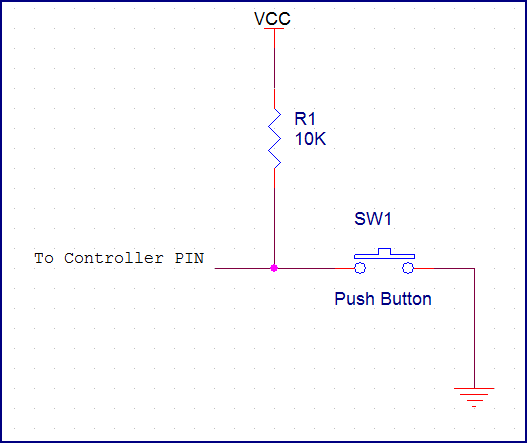
\includegraphics{/home/milav/Codes/MPMC/assets/imgs/181001_MCU_Question_Bank_Solved_html_de2ea01722e2ce88.png}
\caption{}
\end{figure}

\begin{enumerate}
\def\labelenumi{\arabic{enumi}.}
\item
  \textbf{Connect the Pushbutton:} One pin of the pushbutton is
  connected to an input port pin on the 8051 (let's say P1.0). The other
  pin is connected to ground (GND).
\item
  \textbf{Pull-up Resistor:} Connect a pull-up resistor (10K ohms is
  typical) between the pushbutton's input pin and VCC (power supply).
  This ensures the input pin reads a definite HIGH when the button is
  not pressed.
\end{enumerate}

\textbf{Logic}

\begin{itemize}
\item
  \textbf{Pressed:} When pressed, the button connects the input pin to
  GND, reading a logic LOW (0).
\item
  \textbf{Released:} When released, the pull-up resistor pulls the input
  pin HIGH (1).
\end{itemize}

\textbf{Assembly Code}

\begin{Shaded}
\begin{Highlighting}[]
\NormalTok{;Assuming pushbutton is connected to P1.0}

\NormalTok{MAIN\_LOOP:}
\NormalTok{    JB P1.0, BUTTON\_PRESSED   ; Jump if button is pressed (low)}
\NormalTok{    ; ... (Code to execute when the button is NOT pressed)}
\NormalTok{    JMP MAIN\_LOOP}

\NormalTok{BUTTON\_PRESSED:}
\NormalTok{    ; ... (Code to execute when the button IS pressed)}
\NormalTok{    JMP MAIN\_LOOP}
\end{Highlighting}
\end{Shaded}

\textbf{Explanation (Assembly):}

\begin{itemize}
\item
  \textbf{JB:} "Jump if Bit" checks the specified bit (P1.0).
\item
  \textbf{MAIN\_LOOP:} Continuously polls the button state.
\item
  \textbf{BUTTON\_PRESSED:} This section executes if the button is
  pressed.
\end{itemize}

\textbf{C Code}

\begin{Shaded}
\begin{Highlighting}[]
\PreprocessorTok{\#include }\ImportTok{\textless{}reg51.h\textgreater{}}\PreprocessorTok{  }\CommentTok{// Assuming 8051 header file}

\NormalTok{sbit BUTTON }\OperatorTok{=}\NormalTok{ P1}\OperatorTok{\^{}}\DecValTok{0}\OperatorTok{;} \CommentTok{// Assuming button connected to P1.0}

\DataTypeTok{void}\NormalTok{ main}\OperatorTok{()} \OperatorTok{\{}
    \ControlFlowTok{while}\OperatorTok{(}\DecValTok{1}\OperatorTok{)} \OperatorTok{\{}
        \ControlFlowTok{if}\OperatorTok{(}\NormalTok{BUTTON }\OperatorTok{==} \DecValTok{0}\OperatorTok{)} \OperatorTok{\{} \CommentTok{// Button pressed}
            \CommentTok{// ... (Code to execute when button is pressed)}
        \OperatorTok{\}} \ControlFlowTok{else} \OperatorTok{\{}
            \CommentTok{// ... (Code to execute when button is not pressed)}
        \OperatorTok{\}}
    \OperatorTok{\}}
\OperatorTok{\}}
\end{Highlighting}
\end{Shaded}

\textbf{Explanation (C):}

\begin{itemize}
\item
  \textbf{sbit:} Defines a single bit variable for easy access.
\item
  \textbf{while(1):} Creates an infinite loop.
\item
  \textbf{if/else:} Checks the button state and executes appropriate
  code blocks.
\end{itemize}

\textbf{Remember:}

\begin{itemize}
\item
  \textbf{Replace placeholders:} Change '...' in the code blocks with
  the actual actions you want to perform when the button is pressed or
  not pressed (like turning an LED on/off, etc.).
\item
  \textbf{Debouncing:} In real-world scenarios, you'll likely need to
  add debouncing code (software or a small delay circuit) to prevent
  false readings due to mechanical bouncing of the button contacts.
\end{itemize}

\hypertarget{512-dip-switch}{%
\subsubsection{5.1.2. DIP Switch}\label{512-dip-switch}}

\textbf{Hardware Setup}

\begin{figure}
\centering
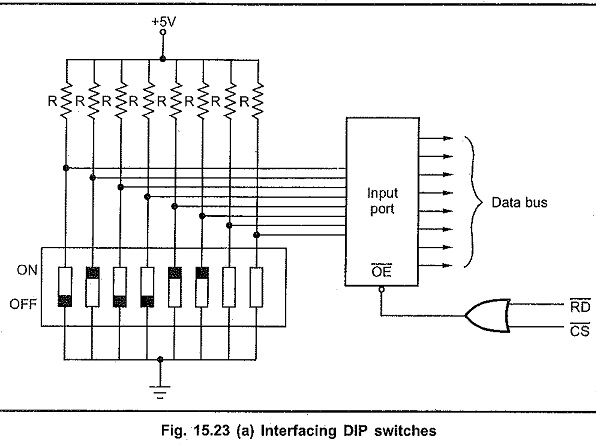
\includegraphics{/home/milav/Codes/MPMC/assets/imgs/181001_MCU_Question_Bank_Solved_html_e23e4e6ed8c25d45.png}
\caption{}
\end{figure}

\begin{enumerate}
\def\labelenumi{\arabic{enumi}.}
\item
  \textbf{Connect the DIP Switch:} Connect one side of each switch in
  the DIP package to separate input pins on the 8051 microcontroller
  (for example, P1.0 through P1.7 for 8 switches).
\item
  \textbf{Pull-up/Pull-down Resistors:} Depending on your DIP switch
  configuration, you'll need one of the following:

  \begin{itemize}
  \item
    \textbf{Pull-up resistors:} If your DIP switches connect to ground
    when ON, connect pull-up resistors (around 10K ohms) between each
    switch pin and VCC.
  \item
    \textbf{Pull-down resistors:} If your DIP switches connect to VCC
    when ON, connect pull-down resistors between each switch pin and
    ground.
  \end{itemize}
\end{enumerate}

\textbf{Logic}

\begin{itemize}
\item
  \textbf{Switch ON:} Provides a definite HIGH (1) or a definite LOW (0)
  to the input pin, depending on your resistor configuration.
\item
  \textbf{Switch OFF:} The resistor pulls the input pin to the opposite
  state.
\end{itemize}

\textbf{Assembly Code}

\begin{Shaded}
\begin{Highlighting}[]
\NormalTok{;Assuming DIP switch connected to Port 1 (P1)}

\NormalTok{MOV A, P1       ; Read the entire port at once}
\NormalTok{; ... Process the input based on individual bits in register A}
\NormalTok{JMP MAIN\_LOOP   ; Continue execution}
\end{Highlighting}
\end{Shaded}

\textbf{Explanation (Assembly):}

\begin{itemize}
\item
  \textbf{MOV A, P1:} Reads the state of all DIP switch pins connected
  to Port 1.
\item
  Individual bits in the Accumulator (A) now represent the switch
  positions. You'll need logic to isolate and handle these bits
  according to your desired functionality.
\end{itemize}

\textbf{C Code}

\begin{Shaded}
\begin{Highlighting}[]
\PreprocessorTok{\#include }\ImportTok{\textless{}reg51.h\textgreater{}}\PreprocessorTok{ }\CommentTok{// Assuming 8051 header file}

\DataTypeTok{unsigned} \DataTypeTok{char}\NormalTok{ DIP\_value}\OperatorTok{;} \CommentTok{// Variable to store DIP switch state}

\DataTypeTok{void}\NormalTok{ main}\OperatorTok{()} \OperatorTok{\{}
    \ControlFlowTok{while}\OperatorTok{(}\DecValTok{1}\OperatorTok{)} \OperatorTok{\{}
\NormalTok{        DIP\_value }\OperatorTok{=}\NormalTok{ P1}\OperatorTok{;} \CommentTok{// Read the value of Port 1}
        \CommentTok{// ... (Process DIP\_value based on bit positions)}
    \OperatorTok{\}}
\OperatorTok{\}}
\end{Highlighting}
\end{Shaded}

\textbf{Explanation (C):}

\begin{itemize}
\item
  \textbf{DIP\_value:} This variable holds the current state of the DIP
  switches.
\item
  \textbf{P1:} Reading the port directly gives you the switch states.
\item
  Individual bits of \texttt{DIP\_value} represent switches. Write logic
  to handle them according to your needs.
\end{itemize}

\textbf{Important Points}

\begin{itemize}
\item
  \textbf{Adapting the Code:} Modify the bit handling logic in the code
  examples to match the desired functionality based on your DIP switch
  arrangement.
\item
  \textbf{Masking (Assembly):} Use bitwise operations (AND, OR) to
  isolate specific bits if needed.
\item
  \textbf{Bit-shifting (C):} Use bit shifts
  (\texttt{\textgreater{}\textgreater{}} or
  \texttt{\textless{}\textless{}}) to check or manipulate individual
  switch states.
\end{itemize}

\textbf{Example: Turn on LED connected to P2.0 if DIP switch 1 is ON}

\textbf{Assembly:}

\begin{Shaded}
\begin{Highlighting}[]
\NormalTok{ANL A, \#01H   ; Mask all bits except bit 0 (representing DIP switch 1)}
\NormalTok{JZ LED\_OFF    ; Jump to LED\_OFF if switch is OFF}
\NormalTok{SETB P2.0     ; Turn LED ON}
\NormalTok{LED\_OFF:}
\NormalTok{   ;....}
\end{Highlighting}
\end{Shaded}

\textbf{C:}

\begin{Shaded}
\begin{Highlighting}[]
\ControlFlowTok{if} \OperatorTok{(}\NormalTok{DIP\_value }\OperatorTok{\&} \BaseNTok{0x01}\OperatorTok{)} \OperatorTok{\{} \CommentTok{// Check if bit 0 is set}
\NormalTok{    P2}\OperatorTok{\^{}}\DecValTok{0} \OperatorTok{=} \DecValTok{1}\OperatorTok{;}  \CommentTok{// Turn LED ON}
\OperatorTok{\}} \ControlFlowTok{else} \OperatorTok{\{}
\NormalTok{    P2}\OperatorTok{\^{}}\DecValTok{0} \OperatorTok{=} \DecValTok{0}\OperatorTok{;}  \CommentTok{// Turn LED OFF}
\OperatorTok{\}}
\end{Highlighting}
\end{Shaded}

\hypertarget{513-keypad-interfacing}{%
\subsubsection{5.1.3. Keypad Interfacing}\label{513-keypad-interfacing}}

\textbf{Hardware Setup}

\begin{figure}
\centering
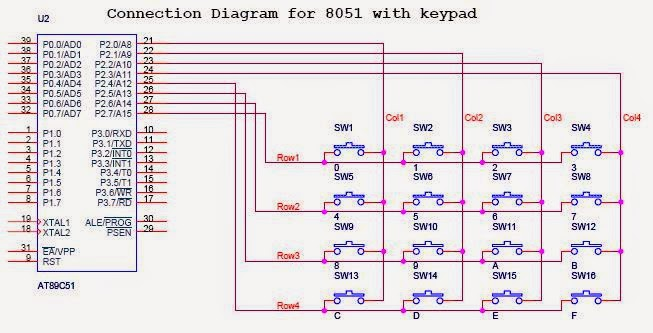
\includegraphics{/home/milav/Codes/MPMC/assets/imgs/181001_MCU_Question_Bank_Solved_html_328066646485eb64.png}
\caption{}
\end{figure}

\begin{itemize}
\item
  \textbf{Keypad Connections:}

  \begin{itemize}
  \item
    Columns: Connect the four column wires of the keypad to pins P2.0 -
    P2.3.
  \item
    Rows: Connect the four row wires of the keypad to pins P2.4 - P2.7.
  \end{itemize}
\item
  \textbf{Pull-up Resistors:} Add pull-up resistors (around 10K ohms)
  between each column pin (P2.0-P2.3) and VCC. These ensure definite
  HIGH signals on the columns when no key is pressed.
\end{itemize}

\textbf{Key Scanning Logic}

\begin{enumerate}
\def\labelenumi{\arabic{enumi}.}
\item
  \textbf{Initialize:} Configure the column pins (P2.0-P2.3) as outputs
  and the row pins (P2.4-P2.7) as inputs.
\item
  \textbf{Column Drive:} Sequentially drive one column LOW at a time,
  keeping the others HIGH.
\item
  \textbf{Row Read:} Read the state of the row pins. If any row pin is
  LOW, it indicates a keypress at the intersection of the active column
  and the detected row.
\item
  \textbf{Debouncing:} Implement a short delay or debouncing algorithm
  to avoid false readings due to keypress bounce.
\end{enumerate}

\textbf{Assembly Code}

\begin{Shaded}
\begin{Highlighting}[]
\NormalTok{MOV P2, \#0FH     ; Initialize columns as output, rows as input}

\NormalTok{KEY\_SCAN:}
\NormalTok{    FOR EACH COLUMN:  ; Iterate through columns 0{-}3}
\NormalTok{        MOV A, COLUMN\_PATTERN ; Load pattern to drive one column low}
\NormalTok{        MOV P2, A             ; Apply pattern to columns}
\NormalTok{        MOV A, P2             ; Read row inputs}
\NormalTok{        ; ... (Check rows for LOW, determine pressed key, debounce)}
\end{Highlighting}
\end{Shaded}

Replace \texttt{COLUMN\_PATTERN} with values like 0x0E, 0x0D, 0x0B, 0x07
to activate one column at a time.

\textbf{C Code}

\begin{Shaded}
\begin{Highlighting}[]
\PreprocessorTok{\#include }\ImportTok{\textless{}reg51.h\textgreater{}}

\DataTypeTok{const} \DataTypeTok{unsigned} \DataTypeTok{char}\NormalTok{ col\_pattern}\OperatorTok{[}\DecValTok{4}\OperatorTok{]} \OperatorTok{=} \OperatorTok{\{}\BaseNTok{0x0E}\OperatorTok{,} \BaseNTok{0x0D}\OperatorTok{,} \BaseNTok{0x0B}\OperatorTok{,} \BaseNTok{0x07}\OperatorTok{\};}

\DataTypeTok{void}\NormalTok{ main}\OperatorTok{()} \OperatorTok{\{}
\NormalTok{    P2 }\OperatorTok{=} \BaseNTok{0x0F}\OperatorTok{;}  \CommentTok{// Initialize columns as output, rows as input}

    \ControlFlowTok{while}\OperatorTok{(}\DecValTok{1}\OperatorTok{)} \OperatorTok{\{}
        \ControlFlowTok{for} \OperatorTok{(}\DataTypeTok{int}\NormalTok{ i}\OperatorTok{=}\DecValTok{0}\OperatorTok{;}\NormalTok{ i}\OperatorTok{\textless{}}\DecValTok{4}\OperatorTok{;}\NormalTok{ i}\OperatorTok{++)} \OperatorTok{\{}
\NormalTok{            P2 }\OperatorTok{=}\NormalTok{ col\_pattern}\OperatorTok{[}\NormalTok{i}\OperatorTok{];}
            \ControlFlowTok{if} \OperatorTok{(}\NormalTok{P2 }\OperatorTok{\&} \BaseNTok{0xF0} \OperatorTok{!=} \BaseNTok{0xF0}\OperatorTok{)} \OperatorTok{\{} \CommentTok{// Check if any row is low}
                \CommentTok{// ... (Determine pressed key, debounce)}
            \OperatorTok{\}}
        \OperatorTok{\}}
    \OperatorTok{\}}
\OperatorTok{\}}
\end{Highlighting}
\end{Shaded}

\textbf{Important Notes}

\begin{itemize}
\item
  \textbf{Key Mapping:} Create a lookup table to map row/column
  combinations to their corresponding key values.
\item
  \textbf{Debouncing:} Implement a delay-based or interrupt-based
  debouncing mechanism.
\item
  \textbf{Code Completion:} The provided snippets demonstrate scanning.
  You'll need to add logic to determine the pressed key based on the
  detected row/column and implement debouncing.
\end{itemize}

\hypertarget{514-potentiometer-interfacing}{%
\subsubsection{5.1.4. Potentiometer
Interfacing}\label{514-potentiometer-interfacing}}

\textbf{Hardware Setup}

\begin{enumerate}
\def\labelenumi{\arabic{enumi}.}
\item
  \textbf{Connecting the Potentiometer:}

  \begin{itemize}
  \item
    \textbf{Middle Pin:} Connect the center (wiper) pin of the
    potentiometer to one of the 8051's analog input channels
    (ADC0804/0808).
  \item
    \textbf{Outer Pins:} Connect one outer pin to VCC (+5V) and the
    other to ground (GND).
  \end{itemize}
\item
  \textbf{Connect ADC (ADC0804/0808):}

  \begin{itemize}
  \item
    \textbf{ADC Pins:} Connect its analog input to the potentiometer's
    wiper pin.
  \item
    \textbf{Digital Pins:} Interface it with the 8051 for data transfer,
    clocking, and control signals.
  \end{itemize}
\end{enumerate}

\textbf{How it Works}

\begin{itemize}
\item
  \textbf{Variable Voltage Divider:} The potentiometer acts as a
  variable voltage divider. As you rotate its knob, the output voltage
  on the center pin changes between 0V and 5V.
\item
  \textbf{ADC Conversion:} The ADC (Analog to Digital Converter)
  converts this analog voltage into a digital value that the 8051 can
  understand.
\end{itemize}

\textbf{Assembly Code (ADC0804/0808)}

\begin{Shaded}
\begin{Highlighting}[]
\NormalTok{;Assuming ADC connected to P1, potentiometer to ADC channel 0}

\NormalTok{ADC\_INIT:}
\NormalTok{    ; ... (Initialize ADC settings)}

\NormalTok{READ\_POT\_VALUE:}
\NormalTok{    SETB ADC\_START  ; Signal start of conversion}
\NormalTok{    ; ... (Wait for conversion to complete)}
\NormalTok{    MOV A, P1       ; Read ADC result}
\NormalTok{    ; ... (Utilize the digital value)}
\end{Highlighting}
\end{Shaded}

\textbf{C Code (ADC0804/0808)}

\begin{Shaded}
\begin{Highlighting}[]
\PreprocessorTok{\#include }\ImportTok{\textless{}reg51.h\textgreater{}}

\DataTypeTok{void}\NormalTok{ adc\_init}\OperatorTok{()} \OperatorTok{\{}
   \CommentTok{// ... (Initialize ADC settings)}
\OperatorTok{\}}

\DataTypeTok{unsigned} \DataTypeTok{int}\NormalTok{ read\_adc}\OperatorTok{()} \OperatorTok{\{}
\NormalTok{    ADC\_START }\OperatorTok{=} \DecValTok{1}\OperatorTok{;}  \CommentTok{// Start conversion}
    \CommentTok{// ... (Wait for conversion to complete)}
    \ControlFlowTok{return}\NormalTok{ P1}\OperatorTok{;}      \CommentTok{// Read ADC result}
\OperatorTok{\}}

\DataTypeTok{void}\NormalTok{ main}\OperatorTok{()} \OperatorTok{\{}
    \DataTypeTok{unsigned} \DataTypeTok{int}\NormalTok{ pot\_value}\OperatorTok{;}

\NormalTok{    adc\_init}\OperatorTok{();}

    \ControlFlowTok{while} \OperatorTok{(}\DecValTok{1}\OperatorTok{)} \OperatorTok{\{}
\NormalTok{        pot\_value }\OperatorTok{=}\NormalTok{ read\_adc}\OperatorTok{();}
        \CommentTok{// ... (Utilize pot\_value)}
    \OperatorTok{\}}
\OperatorTok{\}}
\end{Highlighting}
\end{Shaded}

\textbf{Important Considerations}

\begin{itemize}
\item
  \textbf{ADC Resolution:} The digital value from the ADC (0-1023 for
  10-bit resolution) represents the position of the potentiometer's
  wiper. You might need to scale or map this value to a meaningful range
  within your application.
\item
  \textbf{ADC Control:} Refer to your ADC0804/0808 datasheet for
  specific instructions and registers to set up the ADC correctly.
\end{itemize}

\textbf{Examples of Usage}

\begin{itemize}
\item
  \textbf{Brightness control:} Adjust the brightness of an LED.
\item
  \textbf{Speed Control:} Control the speed of a motor.
\item
  \textbf{Menu Navigation:} Use it as an analog input for menu
  selection.
\end{itemize}

\hypertarget{515-lm35-temperature-sensor}{%
\subsubsection{5.1.5. LM35 Temperature
Sensor}\label{515-lm35-temperature-sensor}}

\textbf{LM35 Basics}

\begin{itemize}
\item
  Analog temperature sensor
\item
  Output voltage is directly proportional to temperature in degrees
  Celsius (10mV/°C)
\item
  Example: 250mV output = 25°C
\end{itemize}

\textbf{Hardware Setup}

\begin{figure}
\centering
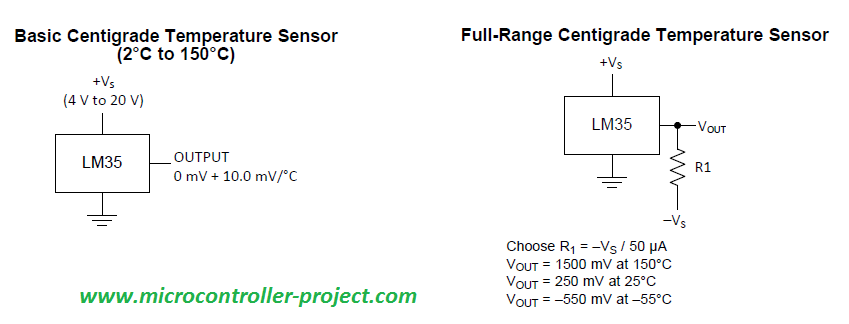
\includegraphics{/home/milav/Codes/MPMC/assets/imgs/181001_MCU_Question_Bank_Solved_html_8b3244abea729276.png}
\caption{}
\end{figure}

\begin{enumerate}
\def\labelenumi{\arabic{enumi}.}
\item
  \textbf{Connect the LM35:}

  \begin{itemize}
  \item
    VCC: Connect to the 8051's power supply (+5V)
  \item
    Output: Connect the LM35's output pin to an analog input channel on
    the ADC0804/0808 ADC chip.
  \item
    GND: Connect to a common ground.
  \end{itemize}
\item
  \textbf{Connect the ADC0804/0808:}

  \begin{itemize}
  \item
    ADC Pins: Connect its analog input to the LM35 output.
  \item
    Digital Pins: Interface the ADC's data, clock, and control pins with
    the 8051 microcontroller.
  \end{itemize}
\end{enumerate}

\textbf{ADC Logic}

\begin{enumerate}
\def\labelenumi{\arabic{enumi}.}
\item
  \textbf{Initialization:} Configure the ADC (resolution, conversion
  mode, etc.).
\item
  \textbf{Start Conversion:} Send a command to the ADC to initiate a
  conversion of the LM35's analog voltage.
\item
  \textbf{Read Digital Result:} Once the conversion is complete, read
  the digital output from the ADC. This digital value represents the
  temperature.
\item
  \textbf{Conversion to Degrees Celsius:} Scale the digital value based
  on the ADC's resolution and the LM35's output characteristics
  (10mV/°C).
\end{enumerate}

\textbf{Assembly Code (ADC0804/0808)}

\begin{Shaded}
\begin{Highlighting}[]
\NormalTok{;Assuming ADC connected to P1, LM35 connected to ADC channel 0}

\NormalTok{ADC\_INIT:}
\NormalTok{    ; ... (Initialize ADC settings)}

\NormalTok{START\_CONV:}
\NormalTok{    SETB ADC\_START  ; Signal start of conversion}
\NormalTok{    ; ... (Wait for conversion to complete)}

\NormalTok{READ\_RESULT:}
\NormalTok{    MOV A, P1      ; Read ADC result}
\NormalTok{    ; ... (Calculate temperature in Celsius)}
\end{Highlighting}
\end{Shaded}

\textbf{C Code (ADC0804/0808)}

\begin{Shaded}
\begin{Highlighting}[]
\PreprocessorTok{\#include }\ImportTok{\textless{}reg51.h\textgreater{}}

\DataTypeTok{void}\NormalTok{ adc\_init}\OperatorTok{()} \OperatorTok{\{}
   \CommentTok{// ... (Initialize ADC settings)}
\OperatorTok{\}}

\DataTypeTok{unsigned} \DataTypeTok{int}\NormalTok{ read\_adc}\OperatorTok{()} \OperatorTok{\{}
\NormalTok{    ADC\_START }\OperatorTok{=} \DecValTok{1}\OperatorTok{;}  \CommentTok{// Start conversion}
    \CommentTok{// ... (Wait for conversion to complete)}
    \ControlFlowTok{return}\NormalTok{ P1}\OperatorTok{;}      \CommentTok{// Read ADC result}
\OperatorTok{\}}

\DataTypeTok{void}\NormalTok{ main}\OperatorTok{()} \OperatorTok{\{}
    \DataTypeTok{unsigned} \DataTypeTok{int}\NormalTok{ adc\_value}\OperatorTok{;}
    \DataTypeTok{float}\NormalTok{ temperature}\OperatorTok{;}

\NormalTok{    adc\_init}\OperatorTok{();}

    \ControlFlowTok{while} \OperatorTok{(}\DecValTok{1}\OperatorTok{)} \OperatorTok{\{}
\NormalTok{        adc\_value }\OperatorTok{=}\NormalTok{ read\_adc}\OperatorTok{();}
\NormalTok{        temperature }\OperatorTok{=}\NormalTok{ adc\_value }\OperatorTok{*} \OperatorTok{(}\FloatTok{5.0} \OperatorTok{/} \DecValTok{1024}\OperatorTok{)} \OperatorTok{*} \DecValTok{100}\OperatorTok{;} \CommentTok{// Calculate temperature}
        \CommentTok{// ... (Display or utilize temperature value)}
    \OperatorTok{\}}
\OperatorTok{\}}
\end{Highlighting}
\end{Shaded}

\textbf{Notes:}

\begin{itemize}
\item
  \textbf{ADC Driver:} You'll likely need specific instructions on
  controlling the ADC0804/0808, which will depend on how it's interfaced
  with the 8051.
\item
  \textbf{Calculation:} In the C code, the calculation assumes a 10-bit
  ADC and a 5V reference voltage.
\item
  \textbf{Code is Simplified:} This omits error handling and some setup
  details.
\end{itemize}

\hypertarget{52-interfacing-output-devices-or-actuators}{%
\subsection{5.2. Interfacing Output Devices or
Actuators}\label{52-interfacing-output-devices-or-actuators}}

\hypertarget{521-leds}{%
\subsubsection{5.2.1. LEDs}\label{521-leds}}

\textbf{Hardware Setup}

\begin{figure}
\centering
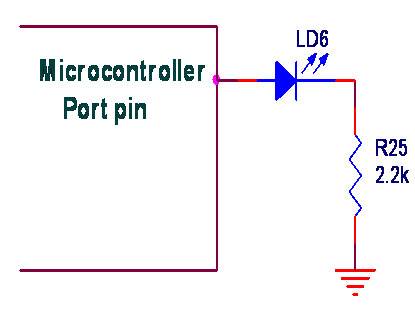
\includegraphics{/home/milav/Codes/MPMC/assets/imgs/181001_MCU_Question_Bank_Solved_html_49368ac6f54d1722.png}
\caption{}
\end{figure}

\begin{enumerate}
\def\labelenumi{\arabic{enumi}.}
\item
  \textbf{Connect LED:} Connect the longer leg (anode) of the LED to an
  I/O pin of the 8051 (let's say P1.0) through a current-limiting
  resistor (around 220 ohms). Connect the shorter leg (cathode) to
  ground (GND).
\end{enumerate}

\textbf{Logic}

\begin{itemize}
\item
  \textbf{ON:} Drive the I/O pin HIGH (1) to turn the LED on.
\item
  \textbf{OFF:} Drive the I/O pin LOW (0) to turn the LED off.
\end{itemize}

\textbf{Assembly Code (Blinking LED)}

\begin{Shaded}
\begin{Highlighting}[]
\NormalTok{;Assuming LED connected to P1.0}

\NormalTok{MOV P1, \#00H    ; Initialize port P1 as output}

\NormalTok{BLINK\_LOOP:}
\NormalTok{    SETB P1.0   ; Turn LED ON}
\NormalTok{    CALL DELAY  ; Call a delay subroutine}
\NormalTok{    CLR P1.0    ; Turn LED OFF}
\NormalTok{    CALL DELAY  ; Another delay}
\NormalTok{    JMP BLINK\_LOOP}

\NormalTok{DELAY:          ; Simple delay subroutine}
\NormalTok{    MOV R5, \#50 ; Adjust these values for}
\NormalTok{    MOV R6, \#200; ...desired delay length}
\NormalTok{DLY\_LOOP:}
\NormalTok{    DJNZ R6, DLY\_LOOP}
\NormalTok{    DJNZ R5, DLY\_LOOP}
\NormalTok{    RET}
\end{Highlighting}
\end{Shaded}

\textbf{Explanation (Assembly)}

\begin{itemize}
\item
  \textbf{MOV P1, \#00H:} Initializes port P1 as output.
\item
  \textbf{SETB/CLR:} Controls the LED (ON/OFF)
\item
  \textbf{CALL DELAY:} Creates a delay between LED state changes.
\item
  \textbf{DELAY subroutine:} Provides a simple adjustable delay.
\end{itemize}

\textbf{C Code (Blinking LED)}

\begin{Shaded}
\begin{Highlighting}[]
\PreprocessorTok{\#include }\ImportTok{\textless{}reg51.h\textgreater{}}

\NormalTok{sbit LED }\OperatorTok{=}\NormalTok{ P1}\OperatorTok{\^{}}\DecValTok{0}\OperatorTok{;}    \CommentTok{// Assuming LED connected to P1.0}

\DataTypeTok{void}\NormalTok{ delay}\OperatorTok{(}\DataTypeTok{unsigned} \DataTypeTok{int}\NormalTok{ ms}\OperatorTok{)} \OperatorTok{\{}
    \DataTypeTok{unsigned} \DataTypeTok{int}\NormalTok{ i}\OperatorTok{,}\NormalTok{ j}\OperatorTok{;}
    \ControlFlowTok{for} \OperatorTok{(}\NormalTok{i }\OperatorTok{=} \DecValTok{0}\OperatorTok{;}\NormalTok{ i }\OperatorTok{\textless{}}\NormalTok{ ms}\OperatorTok{;}\NormalTok{ i}\OperatorTok{++)} \OperatorTok{\{}
        \ControlFlowTok{for} \OperatorTok{(}\NormalTok{j }\OperatorTok{=} \DecValTok{0}\OperatorTok{;}\NormalTok{ j }\OperatorTok{\textless{}} \DecValTok{1275}\OperatorTok{;}\NormalTok{ j}\OperatorTok{++);}
    \OperatorTok{\}}
\OperatorTok{\}}

\DataTypeTok{void}\NormalTok{ main}\OperatorTok{()} \OperatorTok{\{}
    \ControlFlowTok{while} \OperatorTok{(}\DecValTok{1}\OperatorTok{)} \OperatorTok{\{}
\NormalTok{        LED }\OperatorTok{=} \DecValTok{1}\OperatorTok{;}  \CommentTok{// LED ON}
\NormalTok{        delay}\OperatorTok{(}\DecValTok{500}\OperatorTok{);} \CommentTok{// Delay 500ms}
\NormalTok{        LED }\OperatorTok{=} \DecValTok{0}\OperatorTok{;}  \CommentTok{// LED OFF}
\NormalTok{        delay}\OperatorTok{(}\DecValTok{500}\OperatorTok{);} \CommentTok{// Delay 500ms}
    \OperatorTok{\}}
\OperatorTok{\}}
\end{Highlighting}
\end{Shaded}

\textbf{Explanation (C)}

\begin{itemize}
\item
  \textbf{sbit LED:} Conveniently defines an alias for the LED pin.
\item
  \textbf{delay function:} Creates a software delay.
\item
  \textbf{LED = 1/0:} Turns the LED on and off.
\end{itemize}

\textbf{Key Points:}

\begin{itemize}
\item
  \textbf{Resistor:} Always use a current-limiting resistor with LEDs to
  prevent damage.
\item
  \textbf{Delay:} Adjust delay values to control blink speed.
\item
  \textbf{I/O Configuration:} Ensure the pin connected to the LED is
  configured as output.
\end{itemize}

\hypertarget{5211-blink-8-leds}{%
\paragraph{5.2.1.1. Blink 8 LEDs}\label{5211-blink-8-leds}}

\textbf{Hardware Setup}

\begin{figure}
\centering
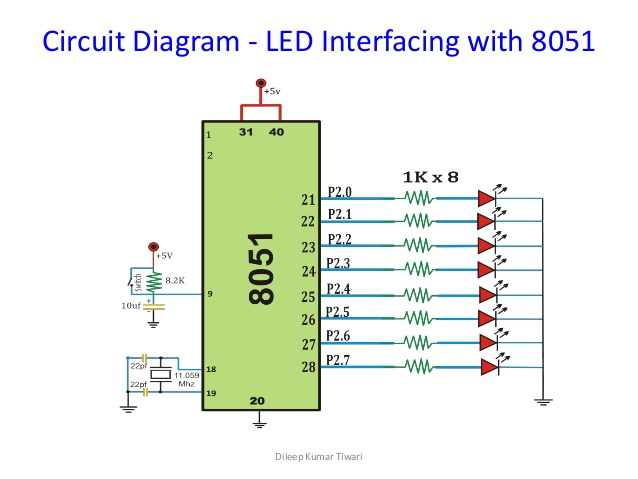
\includegraphics{/home/milav/Codes/MPMC/assets/imgs/181001_MCU_Question_Bank_Solved_html_e163929df693a819.png}
\caption{}
\end{figure}

\begin{enumerate}
\def\labelenumi{\arabic{enumi}.}
\item
  \textbf{8 LEDs:} Choose standard LEDs considering the current
  requirements of the 8051's I/O ports.
\item
  \textbf{Current-Limiting Resistors:} Calculate the appropriate
  resistor values for your specific LEDs to prevent damage (search for
  an online "LED resistor calculator" if needed).
\item
  \textbf{8051 Microcontroller:} We'll assume you have an 8051
  development board with an I/O port (e.g., Port 1).
\item
  \textbf{Connections:}

  \begin{itemize}
  \item
    Connect one leg of each LED to a separate pin on Port 1 of the 8051
    (P1.0 to P1.7).
  \item
    Connect the other leg of each LED through a current-limiting
    resistor to ground.
  \end{itemize}
\end{enumerate}

\textbf{Programming (Assembly)}

Here's a simple 8051 assembly program to repeatedly turn the LEDs on and
then off with a delay:

\begin{Shaded}
\begin{Highlighting}[]
\NormalTok{ORG 0000H  ; Program starts at address 0000H}

\NormalTok{MAIN\_LOOP:}
\NormalTok{    MOV A, \#FFH   ; Set all port pins high (LEDs on)}
\NormalTok{    MOV P1, A     ; Send data to Port 1}
\NormalTok{    CALL DELAY    ; Call a delay subroutine}

\NormalTok{    MOV A, \#00H   ; Set all port pins low (LEDs off)}
\NormalTok{    MOV P1, A}
\NormalTok{    CALL DELAY}

\NormalTok{    SJMP MAIN\_LOOP  ; Jump back to the beginning}

\NormalTok{DELAY:  ; Simple delay subroutine {-} adjust for desired time}
\NormalTok{    MOV R0, \#200   ; Adjust these values for timing}
\NormalTok{    MOV R1, \#150}
\NormalTok{DLY\_LOOP: DJNZ R1, DLY\_LOOP}
\NormalTok{          DJNZ R0, DLY\_LOOP}
\NormalTok{          RET  ; Return from subroutine}

\NormalTok{END}
\end{Highlighting}
\end{Shaded}

\textbf{Explanation}

\begin{enumerate}
\def\labelenumi{\arabic{enumi}.}
\item
  \textbf{MAIN\_LOOP:}

  \begin{itemize}
  \item
    \texttt{MOV\ A,\ \#FFH}: Loads the accumulator with FFH (all bits
    1), which will turn all LEDs on.
  \item
    \texttt{MOV\ P1,\ A}: Sends this value to Port 1.
  \item
    \texttt{CALL\ DELAY}: Calls a subroutine to create a delay.
  \item
    \texttt{MOV\ A,\ \#00H}: Loads the accumulator with 00H (all bits
    0), which will turn all LEDs off.
  \item
    \texttt{SJMP\ MAIN\_LOOP}: Creates an infinite loop.
  \end{itemize}
\item
  \textbf{DELAY Subroutine:}

  \begin{itemize}
  \item
    Provides a simple software delay using nested loops. You might want
    a more precise timer-based delay in a real application.
  \end{itemize}
\end{enumerate}

\textbf{Key Points:}

\begin{itemize}
\item
  \textbf{Port Choice:} I used Port 1(P1); adapt the code if you connect
  the LEDs to a different port.
\item
  \textbf{LED Polarity:} If your LEDs light up in the opposite manner,
  reverse the logic (use 00H to turn them on and FFH to turn them off)
\item
  \textbf{Delay Adjustment:} Modify the values in the DELAY subroutine
  to change the on and off duration.
\end{itemize}

\hypertarget{5212-led-fading-using-pwm}{%
\paragraph{5.2.1.2. LED Fading using
PWM}\label{5212-led-fading-using-pwm}}

\textbf{Understanding PWM}

\begin{itemize}
\item
  PWM stands for Pulse Width Modulation.
\item
  It involves rapidly turning a digital pin ON and OFF at varying
  ratios.
\item
  The longer the ON time relative to the OFF time (the duty cycle), the
  brighter the LED appears.
\item
  Our eyes perceive the rapid blinking as different levels of
  brightness.
\end{itemize}

\textbf{Methods for PWM on the 8051}

\begin{enumerate}
\def\labelenumi{\arabic{enumi}.}
\item
  \textbf{Software PWM:}

  \begin{itemize}
  \item
    Control PWM entirely in your code using delays and pin manipulation.
  \item
    Pros: Flexible, doesn't require specific hardware.
  \item
    Cons: Can consume CPU cycles, limiting the complexity of other code
    running simultaneously.
  \end{itemize}
\item
  \textbf{Hardware PWM (Timer Generated):}

  \begin{itemize}
  \item
    Many 8051 variants have built-in timers that can generate PWM
    signals.
  \item
    Pros: Efficient, frees up your CPU for other tasks.
  \item
    Cons: Less flexible, depends on the available timers and their
    features.
  \end{itemize}
\end{enumerate}

\textbf{Implementing Software PWM}

\textbf{Assembly Code}

\begin{Shaded}
\begin{Highlighting}[]
\NormalTok{;Assuming LED is connected to P1.0}

\NormalTok{FADE\_LOOP:}
\NormalTok{    MOV R0, \#0     ; Brightness counter (0{-}255)}
\NormalTok{    MOV TH0, \#HIGH\_TIME ; Load timer with initial high time}
\NormalTok{    MOV TL0, \#LOW\_TIME  ; Load timer with initial low time}

\NormalTok{PWM\_LOOP:}
\NormalTok{    SETB P1.0       ; LED ON}
\NormalTok{    ACALL TIMER\_DELAY}
\NormalTok{    CLR P1.0        ; LED OFF}
\NormalTok{    ACALL TIMER\_DELAY}

\NormalTok{    INC R0          ; Increase brightness}
\NormalTok{    CJNE R0, \#255, PWM\_LOOP ; Loop until max brightness}

\NormalTok{    ; Add code to fade back down if desired}
\NormalTok{    JMP FADE\_LOOP}

\NormalTok{TIMER\_DELAY:}
\NormalTok{    MOV TMOD, \#01   ; Timer0 in mode 1 (16{-}bit)}
\NormalTok{    SETB TR0        ; Start Timer0}
\NormalTok{    JNB TF0, $      ; Wait for overflow flag}
\NormalTok{    CLR TR0         ; Stop timer}
\NormalTok{    CLR TF0         ; Clear flag}
\NormalTok{    RET}
\end{Highlighting}
\end{Shaded}

\textbf{C Code}

\begin{Shaded}
\begin{Highlighting}[]
\PreprocessorTok{\#include }\ImportTok{\textless{}reg51.h\textgreater{}}

\NormalTok{sbit LED }\OperatorTok{=}\NormalTok{ P1}\OperatorTok{\^{}}\DecValTok{0}\OperatorTok{;}

\DataTypeTok{void}\NormalTok{ timer0\_delay}\OperatorTok{(}\DataTypeTok{unsigned} \DataTypeTok{int}\NormalTok{ us}\OperatorTok{)} \OperatorTok{\{}
\NormalTok{    TMOD }\OperatorTok{=} \BaseNTok{0x01}\OperatorTok{;}  \CommentTok{// Timer0 in mode 1}
    \ControlFlowTok{for} \OperatorTok{(;}\NormalTok{ us}\OperatorTok{\textgreater{}}\DecValTok{0}\OperatorTok{;}\NormalTok{ us}\OperatorTok{{-}{-})} \OperatorTok{\{}
\NormalTok{        TR0 }\OperatorTok{=} \DecValTok{1}\OperatorTok{;}      \CommentTok{// Start timer}
\NormalTok{        TH0 }\OperatorTok{=} \BaseNTok{0xF8}\OperatorTok{;}   \CommentTok{// These values should create}
\NormalTok{        TL0 }\OperatorTok{=} \BaseNTok{0x30}\OperatorTok{;}   \CommentTok{// ... a delay of approximately 1us}
        \ControlFlowTok{while}\OperatorTok{(!}\NormalTok{TF0}\OperatorTok{);}  \CommentTok{// Wait for overflow}
\NormalTok{        TR0 }\OperatorTok{=} \DecValTok{0}\OperatorTok{;}      \CommentTok{// Stop timer}
\NormalTok{        TF0 }\OperatorTok{=} \DecValTok{0}\OperatorTok{;}      \CommentTok{// Clear flag}
    \OperatorTok{\}}
\OperatorTok{\}}

\DataTypeTok{void}\NormalTok{ main}\OperatorTok{()} \OperatorTok{\{}
    \DataTypeTok{unsigned} \DataTypeTok{char}\NormalTok{ brightness }\OperatorTok{=} \DecValTok{0}\OperatorTok{;}
    \DataTypeTok{int}\NormalTok{ direction }\OperatorTok{=} \DecValTok{1}\OperatorTok{;} \CommentTok{// 1 for increasing, {-}1 for decreasing}

    \ControlFlowTok{while}\OperatorTok{(}\DecValTok{1}\OperatorTok{)} \OperatorTok{\{}
\NormalTok{        LED }\OperatorTok{=} \DecValTok{1}\OperatorTok{;}
\NormalTok{        timer0\_delay}\OperatorTok{(}\NormalTok{brightness}\OperatorTok{);}
\NormalTok{        LED }\OperatorTok{=} \DecValTok{0}\OperatorTok{;}
\NormalTok{        timer0\_delay}\OperatorTok{(}\DecValTok{255} \OperatorTok{{-}}\NormalTok{ brightness}\OperatorTok{);}

\NormalTok{        brightness }\OperatorTok{+=}\NormalTok{ direction}\OperatorTok{;}
        \ControlFlowTok{if} \OperatorTok{(}\NormalTok{brightness }\OperatorTok{==} \DecValTok{255} \OperatorTok{||}\NormalTok{ brightness }\OperatorTok{==} \DecValTok{0}\OperatorTok{)} \OperatorTok{\{}
\NormalTok{            direction }\OperatorTok{*=} \OperatorTok{{-}}\DecValTok{1}\OperatorTok{;}  \CommentTok{// Reverse direction}
        \OperatorTok{\}}
    \OperatorTok{\}}
\OperatorTok{\}}
\end{Highlighting}
\end{Shaded}

\hypertarget{522-7-segment-displays}{%
\subsubsection{5.2.2. 7-Segment Displays}\label{522-7-segment-displays}}

\textbf{Assumptions}

\begin{figure}
\centering
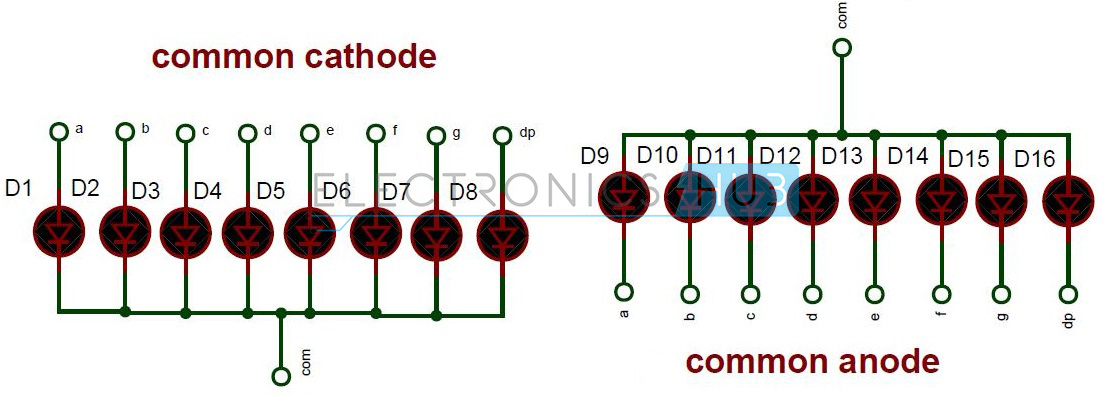
\includegraphics{/home/milav/Codes/MPMC/assets/imgs/181001_MCU_Question_Bank_Solved_html_10b11f2bcaf55e61.png}
\caption{}
\end{figure}

\begin{itemize}
\item
  \textbf{Common Anode Display:} The segments have a common positive
  connection. We'll control them by sinking current (connecting to
  ground) through the 8051's pins.

  \begin{itemize}
  \item
    Adapt the segment patterns if you have a Common Cathode display.
  \end{itemize}
\item
  \textbf{Single Digit:} We'll interface a single digit display. This
  can be extended for multiple digits using multiplexing techniques.
\item
  \textbf{Connections:} We'll assume you'll connect the 7-segment pins
  (a through g) to a port of the 8051 (e.g., Port 1).
\end{itemize}

\textbf{Hardware Setup}

\begin{figure}
\centering
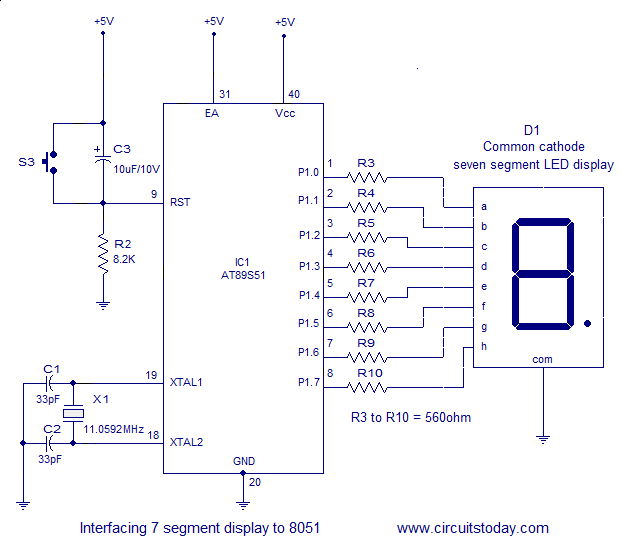
\includegraphics{/home/milav/Codes/MPMC/assets/imgs/181001_MCU_Question_Bank_Solved_html_32bf665d29e7e447.png}
\caption{}
\end{figure}

\begin{enumerate}
\def\labelenumi{\arabic{enumi}.}
\item
  \textbf{7-Segment Display:} Choose a common anode 7-segment LED
  display.
\item
  \textbf{Current-Limiting Resistors:} Calculate and use resistors in
  series with each segment LED to prevent damage. Search for a "LED
  resistor calculator" to find the right values.
\item
  \textbf{Connections:}

  \begin{itemize}
  \item
    Connect the anodes of all segments (a through g) to the
    corresponding pins of Port 1 (P1.0 through P1.6) of the 8051.
  \item
    Connect the common anode pin to the power supply (+5V).
  \item
    Connect each segment's cathode through the resistor to ground.
  \end{itemize}
\end{enumerate}

\textbf{Lookup Table}

Create a lookup table in your program memory that maps the digit you
want to display (0-9) to the corresponding segment patterns:

\begin{Shaded}
\begin{Highlighting}[]
\NormalTok{SEGMENT\_PATTERNS:}
\NormalTok{    DB 0C0H ; Pattern for 0 (abcdefg)}
\NormalTok{    DB 0F9H ; Pattern for 1}
\NormalTok{    DB 0A4H ; Pattern for 2}
\NormalTok{     ; ... Add patterns for 3{-}9}
\end{Highlighting}
\end{Shaded}

Note: For a common anode display, '1' means the segment should be ON, so
it's connected to ground.

\textbf{Assembly Code Example}

\begin{Shaded}
\begin{Highlighting}[]
\NormalTok{ORG 0000H}

\NormalTok{; Assume display is connected to Port 1}
\NormalTok{DISPLAY\_PORT EQU P1}

\NormalTok{; ... (Segment patterns lookup table from above)}

\NormalTok{MAIN\_LOOP:}
\NormalTok{    MOV R0, \#2   ; Example: Load the digit 2 to display}
\NormalTok{    MOV A, @R0   ; Point to the segment pattern in the table}
\NormalTok{    ADD A, SEGMENT\_PATTERNS  ; Calculate the address}
\NormalTok{    MOVC A, @A+DPTR          ; Fetch the segment pattern}
\NormalTok{    MOV DISPLAY\_PORT, A      ;  Send the pattern to the display port}

\NormalTok{    ; ... (Add display refreshing if you want to multiplex multiple digits)}
\NormalTok{END}
\end{Highlighting}
\end{Shaded}

\textbf{Explanation}

\begin{itemize}
\item
  \textbf{Table Usage:} The code loads the digit to be displayed into
  R0, uses indirect addressing to get the corresponding pattern from the
  lookup table, and sends it to the display port.
\item
  \textbf{Multiplexing:} If you have multiple 7-segment displays, you
  need to switch between them rapidly and update the display port
  accordingly to create the illusion they are all on simultaneously.
\end{itemize}

\textbf{Important:}

\begin{itemize}
\item
  \textbf{Port Output:} Ensure the port you use is configured as output.
\item
  \textbf{Resistors:} Don't forget the current-limiting resistors!
\end{itemize}

\hypertarget{523-lcd-interfacing}{%
\subsubsection{5.2.3. LCD Interfacing}\label{523-lcd-interfacing}}

\textbf{Hardware Setup}

\begin{figure}
\centering
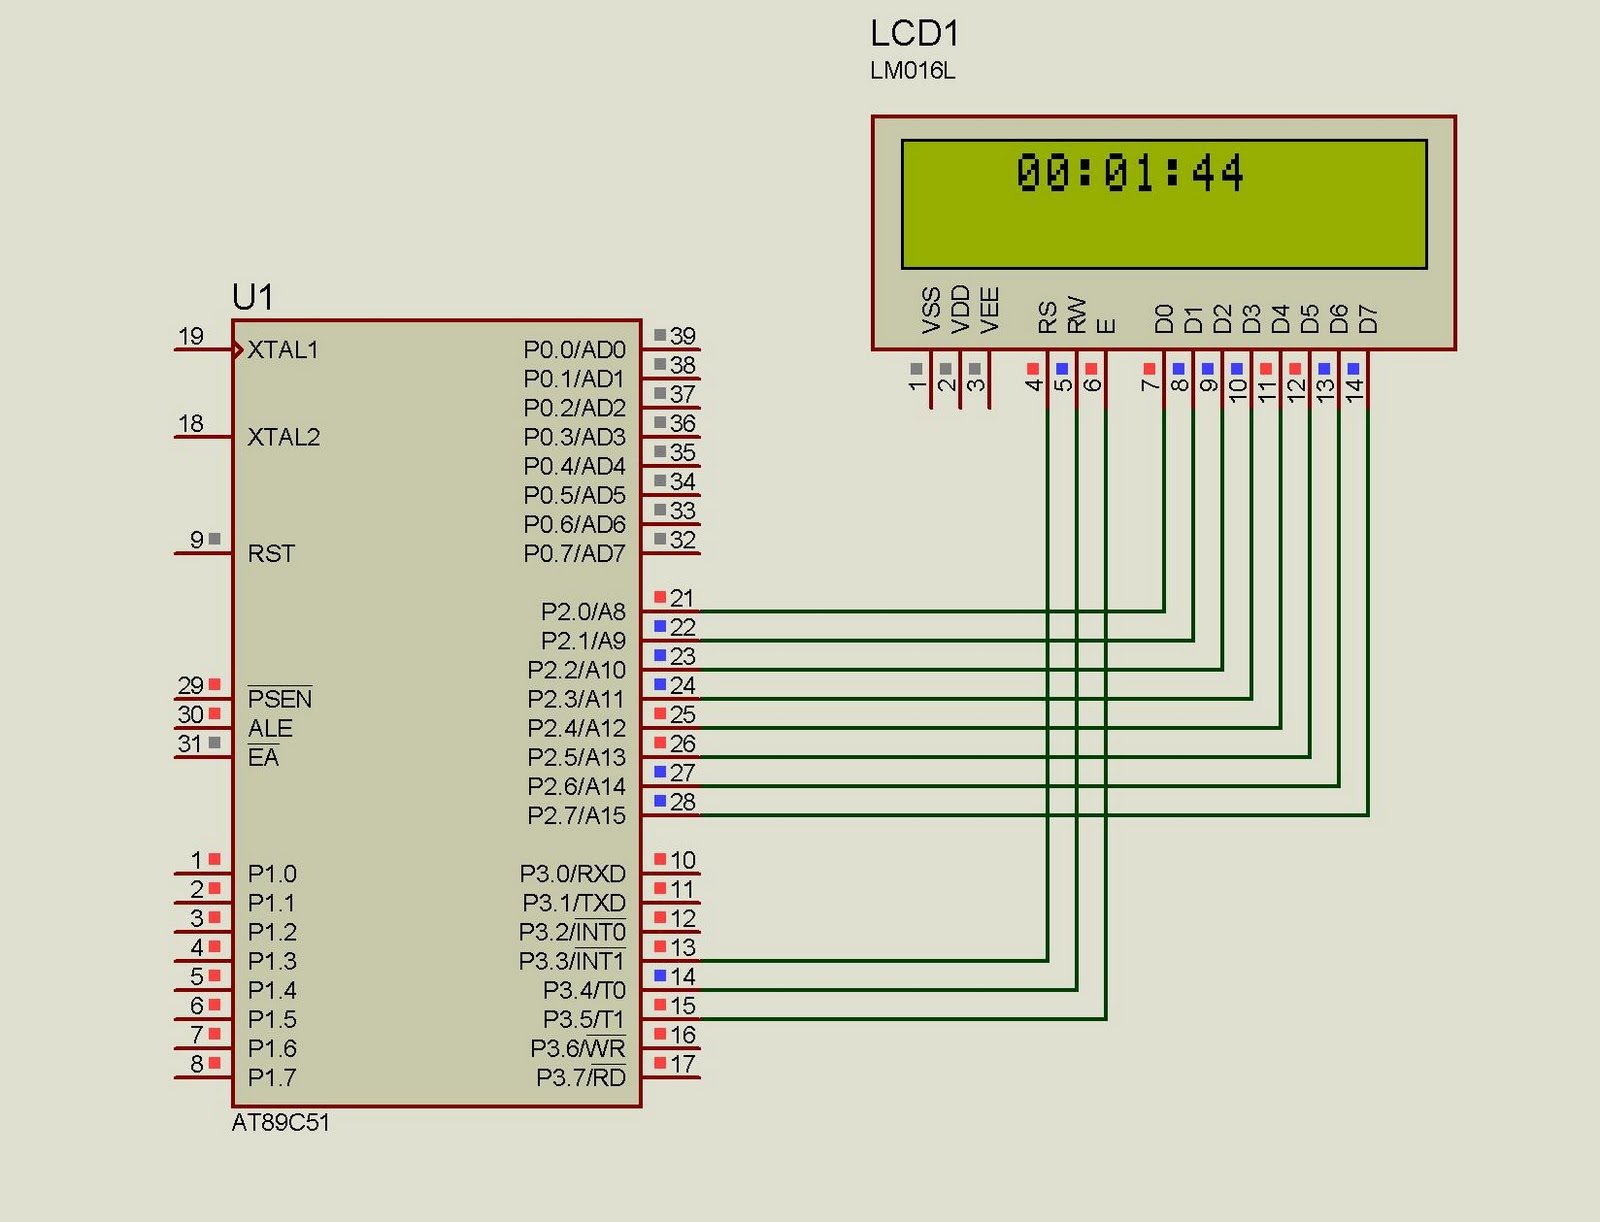
\includegraphics{/home/milav/Codes/MPMC/assets/imgs/181001_MCU_Question_Bank_Solved_html_cb8b02fcff93f213.png}
\caption{}
\end{figure}

\begin{itemize}
\item
  \textbf{LCD:} We'll assume a standard 16x2 character LCD module with a
  common HD44780 compatible controller.
\item
  \textbf{Connections:}

  \begin{itemize}
  \item
    \textbf{Data Pins (D0-D7):} Connect to an 8051 I/O Port (e.g., Port
    2)
  \item
    \textbf{Control Pins:}

    \begin{itemize}
    \item
      RS (Register Select): Connect to an 8051 pin (e.g., P1.0)
    \item
      RW (Read/Write): Connect to an 8051 pin (e.g., P1.1)
    \item
      E (Enable): Connect to an 8051 pin (e.g., P1.2)
    \end{itemize}
  \item
    \textbf{Contrast Adjustment (Vo):} Connect to a potentiometer for
    controlling display contrast.
  \item
    \textbf{Backlight (if present):} Power according to its
    requirements.
  \end{itemize}
\end{itemize}

\textbf{Assembly Programming}

Here's an 8051 assembly program to initialize the LCD and display
"Welcome":

\begin{Shaded}
\begin{Highlighting}[]
\NormalTok{ORG 0000H}

\NormalTok{; Constants}
\NormalTok{LCD\_PORT EQU P2}
\NormalTok{RS\_PIN   EQU P1.0}
\NormalTok{RW\_PIN   EQU P1.1}
\NormalTok{E\_PIN    EQU P1.2}

\NormalTok{; {-}{-}{-} LCD Initialization {-}{-}{-}}
\NormalTok{LCD\_INIT:}
\NormalTok{    MOV A, \#38H  ; Function set: 8{-}bit, 2 lines, 5x7 font}
\NormalTok{    CALL LCD\_CMD}
\NormalTok{    MOV A, \#0CH  ; Display on, cursor off, no blinking}
\NormalTok{    CALL LCD\_CMD}
\NormalTok{    MOV A, \#01H  ; Clear display}
\NormalTok{    CALL LCD\_CMD}
\NormalTok{    MOV A, \#06H  ; Entry mode: Increment cursor}
\NormalTok{    CALL LCD\_CMD}
\NormalTok{    RET}

\NormalTok{; {-}{-}{-} Send Command to LCD  {-}{-}{-}}
\NormalTok{LCD\_CMD:}
\NormalTok{    CLR RS\_PIN}
\NormalTok{    CLR RW\_PIN}
\NormalTok{    MOV LCD\_PORT, A}
\NormalTok{    SETB E\_PIN     ; Pulse Enable}
\NormalTok{    CLR E\_PIN}
\NormalTok{    CALL DELAY     ; Small delay (important for LCD)}
\NormalTok{    RET}

\NormalTok{; {-}{-}{-} Send Data (Character) to LCD {-}{-}{-}}
\NormalTok{LCD\_DATA:}
\NormalTok{    SETB RS\_PIN}
\NormalTok{    CLR RW\_PIN}
\NormalTok{    MOV LCD\_PORT, A}
\NormalTok{    SETB E\_PIN      ; Pulse Enable}
\NormalTok{    CLR E\_PIN}
\NormalTok{    CALL DELAY      ; Small delay}
\NormalTok{    RET}

\NormalTok{; {-}{-}{-} Simple Delay Subroutine {-}{-}{-}}
\NormalTok{DELAY:}
\NormalTok{    MOV R5, \#50    ; Adjust these for approximate delay}
\NormalTok{    DLOOP: MOV R6, \#200}
\NormalTok{           DJNZ R6, DLOOP}
\NormalTok{           DJNZ R5, DLOOP}
\NormalTok{           RET}

\NormalTok{; {-}{-} Main Program {-}{-}}
\NormalTok{MAIN:}
\NormalTok{    CALL LCD\_INIT}

\NormalTok{    MOV A, \#80H     ; Set cursor to first line, first position}
\NormalTok{    CALL LCD\_CMD}

\NormalTok{    MOV A, \#\textquotesingle{}W\textquotesingle{}    ; Load characters to send}
\NormalTok{    CALL LCD\_DATA}
\NormalTok{    MOV A, \#\textquotesingle{}e\textquotesingle{}}
\NormalTok{    CALL LCD\_DATA}
\NormalTok{    MOV A, \#\textquotesingle{}l\textquotesingle{}}
\NormalTok{    CALL LCD\_DATA}
\NormalTok{    ; ... (Send rest of "come")}

\NormalTok{END ; Add an infinite loop if needed for display to stay}
\end{Highlighting}
\end{Shaded}

\textbf{Explanation}

\begin{itemize}
\item
  \textbf{Constants:} \texttt{LCD\_PORT} is defined to make the code
  adaptable if your connections change.
\item
  \textbf{Subroutines:} These encapsulate the interaction details with
  the LCD (sending commands, sending data), making the main program
  cleaner. You'll need to fill in the details of these subroutines
  according to your LCD's datasheet.
\item
  \textbf{Main Program:}

  \begin{itemize}
  \item
    Calls \texttt{LCD\_INIT} to configure the LCD.
  \item
    Sends commands to select the desired display mode (2 lines, 5x7
    font) and clear the display.
  \item
    Sends each character of the message "Welcome" to the LCD using
    \texttt{LCD\_DATA}.
  \end{itemize}
\end{itemize}

\textbf{Key Points}

\begin{itemize}
\item
  \textbf{LCD Datasheet:} You MUST adapt the initialization and command
  sequences based on your specific LCD module.
\item
  \textbf{8051 Timing:} You might need short delays within the
  subroutines to ensure the LCD processes commands correctly.
\item
  \textbf{Subroutine Implementation:} The core logic of sending
  commands/data to the LCD involves setting the RS/RW lines, placing
  data on the data port, and pulsing the Enable pin.
\end{itemize}

\hypertarget{524-relays}{%
\subsubsection{5.2.4. Relays}\label{524-relays}}

\textbf{Relays Explained}

\begin{itemize}
\item
  \textbf{Electromagnetic Switches:} Relays are electromechanical
  switches that use an electromagnet to control the opening and closing
  of contacts.
\item
  \textbf{Coil and Contacts:} They consist of a coil, an armature
  (lever), and a set of contacts.
\item
  \textbf{Activation:} When current flows through the coil, it generates
  a magnetic field that attracts the armature, causing the contacts to
  switch states (open or closed).
\end{itemize}

\begin{figure}
\centering
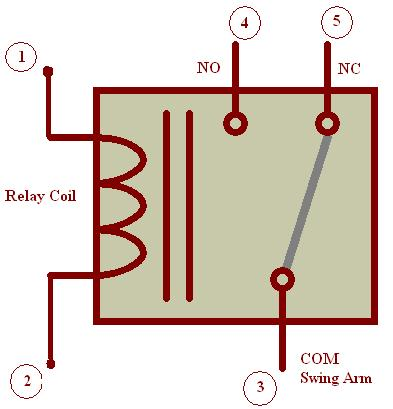
\includegraphics{/home/milav/Codes/MPMC/assets/imgs/181001_MCU_Question_Bank_Solved_html_71f03f4ccf0de505.png}
\caption{}
\end{figure}

\textbf{Interfacing with 8051}

\begin{enumerate}
\def\labelenumi{\arabic{enumi}.}
\item
  \textbf{Driver Circuit:} The 8051 microcontroller cannot directly
  provide the high current needed to operate the relay coil. Therefore,
  a driver circuit is necessary.

  \begin{itemize}
  \item
    \textbf{Transistor:} A common approach is to use a transistor as a
    switch, controlled by the 8051 output pin.
  \item
    \textbf{Driver ICs:} Dedicated driver ICs like the ULN2003 are also
    commonly used for easier interfacing with multiple relays.
  \end{itemize}
\item
  \textbf{Connections:}

  \begin{itemize}
  \item
    Connect the control pin of the transistor (or driver IC) to an
    output pin of the 8051.
  \item
    Connect the relay coil to the collector and emitter of the
    transistor (or the corresponding pins on the driver IC).
  \item
    Connect the relay's common contact to your desired circuit, and the
    normally open (NO) or normally closed (NC) contact based on your
    switching needs.
  \end{itemize}
\end{enumerate}

\begin{figure}
\centering
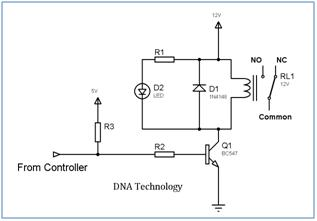
\includegraphics{/home/milav/Codes/MPMC/assets/imgs/181001_MCU_Question_Bank_Solved_html_62d8cd123ac4b469.png}
\caption{}
\end{figure}

\textbf{Assembly Code Example}

\begin{Shaded}
\begin{Highlighting}[]
\NormalTok{ORG 0000H}

\NormalTok{; Define relay control state (low for on)}
\NormalTok{MOV R0, \#00H  ; Relay off initially}

\NormalTok{MAIN\_LOOP:}
\NormalTok{    ; Turn on relay (set P1.0 low)}
\NormalTok{    MOV P1, R0}

\NormalTok{    ; Delay (adjust for desired activation time)}
\NormalTok{    MOV R2, \#100  ; Set delay loop counter}
\NormalTok{    DELAY\_LOOP:}
\NormalTok{        DJNZ R2, DELAY\_LOOP}

\NormalTok{    ; Turn off relay (set P1.0 high)}
\NormalTok{    SETB P1.0   ; Set P1.0 high using SETB instruction}

\NormalTok{    ; Delay (adjust for desired deactivation time)}
\NormalTok{    MOV R2, \#100  ; Set delay loop counter}
\NormalTok{    DELAY\_LOOP:}
\NormalTok{        DJNZ R2, DELAY\_LOOP}

\NormalTok{    JMP MAIN\_LOOP  ; Repeat continuously}
\end{Highlighting}
\end{Shaded}

\textbf{C Code Example}

\begin{Shaded}
\begin{Highlighting}[]
\PreprocessorTok{\#include }\ImportTok{\textless{}reg51.h\textgreater{}}

\NormalTok{sbit RELAY\_CTRL }\OperatorTok{=}\NormalTok{ P1}\OperatorTok{\^{}}\DecValTok{0}\OperatorTok{;}  \CommentTok{// Connect relay control pin to P1.0}

\DataTypeTok{void}\NormalTok{ delay}\OperatorTok{(}\DataTypeTok{unsigned} \DataTypeTok{int}\NormalTok{ ms}\OperatorTok{)} \OperatorTok{\{} \CommentTok{// Simple delay routine}
    \DataTypeTok{unsigned} \DataTypeTok{int}\NormalTok{ i}\OperatorTok{,}\NormalTok{ j}\OperatorTok{;}
    \ControlFlowTok{for} \OperatorTok{(}\NormalTok{i }\OperatorTok{=} \DecValTok{0}\OperatorTok{;}\NormalTok{ i }\OperatorTok{\textless{}}\NormalTok{ ms}\OperatorTok{;}\NormalTok{ i}\OperatorTok{++)} \OperatorTok{\{}
        \ControlFlowTok{for} \OperatorTok{(}\NormalTok{j }\OperatorTok{=} \DecValTok{0}\OperatorTok{;}\NormalTok{ j }\OperatorTok{\textless{}} \DecValTok{1275}\OperatorTok{;}\NormalTok{ j}\OperatorTok{++);}
    \OperatorTok{\}}
\OperatorTok{\}}

\DataTypeTok{void}\NormalTok{ main}\OperatorTok{()} \OperatorTok{\{}
    \ControlFlowTok{while} \OperatorTok{(}\DecValTok{1}\OperatorTok{)} \OperatorTok{\{}
\NormalTok{        RELAY\_CTRL }\OperatorTok{=} \DecValTok{0}\OperatorTok{;}  \CommentTok{// Turn on relay (active low)}
\NormalTok{        delay}\OperatorTok{(}\DecValTok{100}\OperatorTok{);}      \CommentTok{// Adjust delay for desired activation time}

\NormalTok{        RELAY\_CTRL }\OperatorTok{=} \DecValTok{1}\OperatorTok{;}  \CommentTok{// Turn off relay}
\NormalTok{        delay}\OperatorTok{(}\DecValTok{100}\OperatorTok{);}      \CommentTok{// Adjust delay for desired deactivation time}
    \OperatorTok{\}}
\OperatorTok{\}}
\end{Highlighting}
\end{Shaded}

\textbf{Explanation of the Code:}

\begin{itemize}
\item
  \textbf{Relay Control State:} We define a variable (\texttt{R0} in
  assembly, \texttt{RELAY\_CTRL} in C) to represent the relay state
  (on/off).
\item
  \textbf{Main Loop:} The code continuously loops, turning the relay on
  and off with adjustable delays using a simple delay routine.
\item
  \textbf{Assembly:} The \texttt{SETB} instruction is used to directly
  set the P1.0 pin high.
\item
  \textbf{C:} The \texttt{sbit} directive is used to define a bit-level
  controllable variable for the relay control pin.
\end{itemize}

\hypertarget{525-dc-motors}{%
\subsubsection{5.2.5. DC Motors}\label{525-dc-motors}}

\hypertarget{5251-l293d-ic}{%
\paragraph{5.2.5.1. L293D IC}\label{5251-l293d-ic}}

It is a versatile integrated circuit that can be used to drive various
types of DC motors and steppers motors.

\textbf{Key Features:}

\begin{itemize}
\item
  \textbf{Dual H-bridge driver:} It can control two DC motors or one
  bipolar stepper motor simultaneously in both directions (forward and
  reverse) by reversing the polarity of the voltage applied to the
  motor.
\item
  \textbf{Wide operating voltage:} It can operate with a voltage range
  of 4.5V to 36V, making it suitable for various applications.
\item
  \textbf{High current capability:} Each channel can deliver a
  continuous current of up to 600mA, making it suitable for driving
  small to medium-sized DC motors.
\item
  \textbf{Logic level inputs:} The control inputs are compatible with
  digital logic levels (0V to 5V), allowing for easy control with
  microcontrollers like the 8051.
\end{itemize}

\textbf{Pin Configuration:}

\begin{figure}
\centering
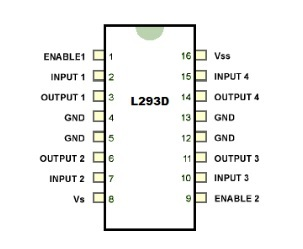
\includegraphics{/home/milav/Codes/MPMC/assets/imgs/181001_MCU_Question_Bank_Solved_html_975eda0bdb235063.png}
\caption{}
\end{figure}

\begin{itemize}
\item
  \textbf{Inputs (2 per channel):}

  \begin{itemize}
  \item
    IN1 and IN2: Control the direction of the connected motor
    (forward/reverse).
  \end{itemize}
\item
  \textbf{Outputs (2 per channel):}

  \begin{itemize}
  \item
    OUT1 and OUT2: Connect to the motor terminals.
  \end{itemize}
\item
  \textbf{Power supply:}

  \begin{itemize}
  \item
    Vcc: Positive power supply (4.5V to 36V).
  \item
    GND: Ground.
  \end{itemize}
\item
  \textbf{Enable pins (optional):}

  \begin{itemize}
  \item
    Enable1 and Enable2: Enable or disable the respective motor driver
    channel.
  \end{itemize}
\end{itemize}

\textbf{Applications:}

\begin{itemize}
\item
  Robot locomotion (driving wheels)
\item
  Controlling conveyor belts
\item
  Operating solenoid valves
\item
  Remote-controlled toys and cars
\end{itemize}

\textbf{How it Works:}

By applying specific high or low logic signals to the IN1 and IN2 pins,
you can control the direction and rotation of the connected DC motor.
The L293D internally manages the power flow to the motor terminals (OUT1
and OUT2) based on the input signals.

\hypertarget{5252-dc-motor-interfacing-with-8051}{%
\paragraph{5.2.5.2. DC Motor Interfacing with
8051}\label{5252-dc-motor-interfacing-with-8051}}

\textbf{Hardware Connections:}

\begin{figure}
\centering
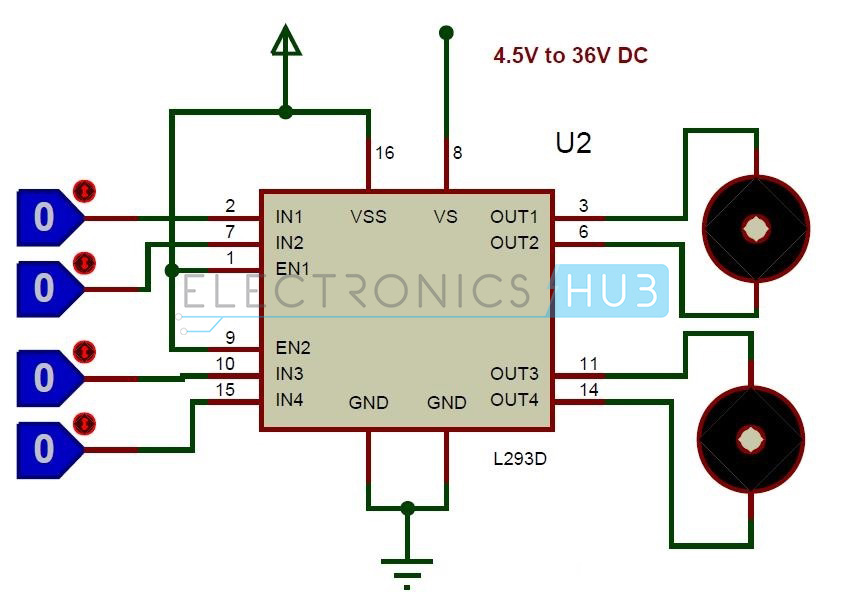
\includegraphics{/home/milav/Codes/MPMC/assets/imgs/181001_MCU_Question_Bank_Solved_html_caf5d6f29475a454.png}
\caption{}
\end{figure}

\begin{enumerate}
\def\labelenumi{\arabic{enumi}.}
\item
  \textbf{Connect the L293D motor driver:}

  \begin{itemize}
  \item
    Vcc of the L293D to +5V power supply.
  \item
    GND to ground.
  \item
    Connect IN1, IN2, IN3, and IN4 of the L293D to four control pins
    (e.g., P1.0 to P1.3) of the 8051.
  \item
    Connect the motor to the OUT1 and OUT2 pins of the L293D's first
    channel (Channel 1).
  \end{itemize}
\item
  \textbf{Connect the motor supply:}

  \begin{itemize}
  \item
    Connect the positive terminal of the motor to a separate power
    supply (voltage appropriate for your motor, typically 6V to 12V).
  \item
    Connect the negative terminal of the motor to the ground.
  \end{itemize}
\end{enumerate}

\textbf{Assembly Code:}

\begin{Shaded}
\begin{Highlighting}[]
\NormalTok{ORG 0000H}

\NormalTok{; Define motor control states}
\NormalTok{MOV R0, \#01H ; Forward (IN1 = 1, IN2 = 0)}
\NormalTok{MOV R1, \#10H ; Reverse (IN1 = 0, IN2 = 1)}

\NormalTok{MAIN\_LOOP:}
\NormalTok{    MOV P1, R0     ; Set motor direction (forward initially)}

\NormalTok{    ; Delay (adjust for desired speed)}
\NormalTok{    MOV R2, \#100  ; Set delay loop counter}
\NormalTok{    DELAY\_LOOP:}
\NormalTok{        DJNZ R2, DELAY\_LOOP}

\NormalTok{    ; Reverse direction}
\NormalTok{    MOV P1, R1}

\NormalTok{    ; Delay (adjust for desired speed)}
\NormalTok{    MOV R2, \#100  ; Set delay loop counter}
\NormalTok{    DELAY\_LOOP:}
\NormalTok{        DJNZ R2, DELAY\_LOOP}

\NormalTok{    JMP MAIN\_LOOP  ; Repeat continuously}
\end{Highlighting}
\end{Shaded}

\textbf{C Code:}

\begin{Shaded}
\begin{Highlighting}[]
\PreprocessorTok{\#include }\ImportTok{\textless{}reg51.h\textgreater{}}

\NormalTok{sbit IN1 }\OperatorTok{=}\NormalTok{ P1}\OperatorTok{\^{}}\DecValTok{0}\OperatorTok{;}  \CommentTok{// Connect IN1 to P1.0}
\NormalTok{sbit IN2 }\OperatorTok{=}\NormalTok{ P1}\OperatorTok{\^{}}\DecValTok{1}\OperatorTok{;}  \CommentTok{// Connect IN2 to P1.1}

\DataTypeTok{void}\NormalTok{ delay}\OperatorTok{(}\DataTypeTok{unsigned} \DataTypeTok{int}\NormalTok{ ms}\OperatorTok{)} \OperatorTok{\{} \CommentTok{// Simple delay routine}
    \DataTypeTok{unsigned} \DataTypeTok{int}\NormalTok{ i}\OperatorTok{,}\NormalTok{ j}\OperatorTok{;}
    \ControlFlowTok{for} \OperatorTok{(}\NormalTok{i }\OperatorTok{=} \DecValTok{0}\OperatorTok{;}\NormalTok{ i }\OperatorTok{\textless{}}\NormalTok{ ms}\OperatorTok{;}\NormalTok{ i}\OperatorTok{++)} \OperatorTok{\{}
        \ControlFlowTok{for} \OperatorTok{(}\NormalTok{j }\OperatorTok{=} \DecValTok{0}\OperatorTok{;}\NormalTok{ j }\OperatorTok{\textless{}} \DecValTok{1275}\OperatorTok{;}\NormalTok{ j}\OperatorTok{++);}
    \OperatorTok{\}}
\OperatorTok{\}}

\DataTypeTok{void}\NormalTok{ main}\OperatorTok{()} \OperatorTok{\{}
    \ControlFlowTok{while} \OperatorTok{(}\DecValTok{1}\OperatorTok{)} \OperatorTok{\{}
\NormalTok{        IN1 }\OperatorTok{=} \DecValTok{1}\OperatorTok{;}  \CommentTok{// Forward (IN1 = 1, IN2 = 0)}
\NormalTok{        delay}\OperatorTok{(}\DecValTok{100}\OperatorTok{);} \CommentTok{// Adjust delay for desired speed}

\NormalTok{        IN1 }\OperatorTok{=} \DecValTok{0}\OperatorTok{;}  \CommentTok{// Reverse (IN1 = 0, IN2 = 1)}
\NormalTok{        delay}\OperatorTok{(}\DecValTok{100}\OperatorTok{);} \CommentTok{// Adjust delay for desired speed}
    \OperatorTok{\}}
\OperatorTok{\}}
\end{Highlighting}
\end{Shaded}

\textbf{Explanation:}

\begin{enumerate}
\def\labelenumi{\arabic{enumi}.}
\item
  \textbf{Motor Control States:}

  \begin{itemize}
  \item
    We define two variables (\texttt{R0} and \texttt{R1}) in assembly or
    \texttt{sbit} definitions in C to represent the forward and reverse
    motor control states.
  \end{itemize}
\item
  \textbf{Main Loop:}

  \begin{itemize}
  \item
    The code continuously runs in a loop, setting the motor direction
    pin values (P1.0 and P1.1) based on the defined states (\texttt{R0}
    or \texttt{R1}).
  \end{itemize}
\item
  \textbf{Delay:}

  \begin{itemize}
  \item
    A simple delay loop is included to control the duration of each
    direction (forward and reverse).
  \item
    Adjust the delay value (\texttt{\#100} in assembly, \texttt{100} in
    C) to change the motor speed.
  \end{itemize}
\end{enumerate}

\hypertarget{526-stepper-motors}{%
\subsubsection{5.2.6. Stepper Motors}\label{526-stepper-motors}}

\hypertarget{5261-basics-of-stepper-motors}{%
\paragraph{5.2.6.1. Basics of Stepper
Motors}\label{5261-basics-of-stepper-motors}}

\begin{itemize}
\item
  \textbf{Type of Motor:} Stepper motors are brushless DC motors that
  convert electrical pulses into precise, discrete rotational movements.
\item
  \textbf{Steps:} Their unique feature is that the shafts rotate in
  fixed angular increments (steps) rather than continuously. This allows
  for highly accurate positioning without feedback sensors (open-loop
  control).
\item
  \textbf{Stator and Rotor:}

  \begin{itemize}
  \item
    Stator: Stationary part holding multiple electromagnetic coils.
  \item
    Rotor: Typically a permanent magnet that rotates in response to
    energized stator coils.
  \end{itemize}
\end{itemize}

\textbf{Types of Stepper Motors}

\begin{itemize}
\item
  \textbf{Unipolar Stepper Motors}

  \begin{itemize}
  \item
    Most Common
  \item
    Each coil has a center tap.
  \item
    5, 6, or 8 wire configurations possible.
  \end{itemize}
\item
  \textbf{Bipolar Stepper Motors}

  \begin{itemize}
  \item
    No center taps on coils.
  \item
    Require reversing coil currents to change direction.
  \end{itemize}
\end{itemize}

\begin{figure}
\centering
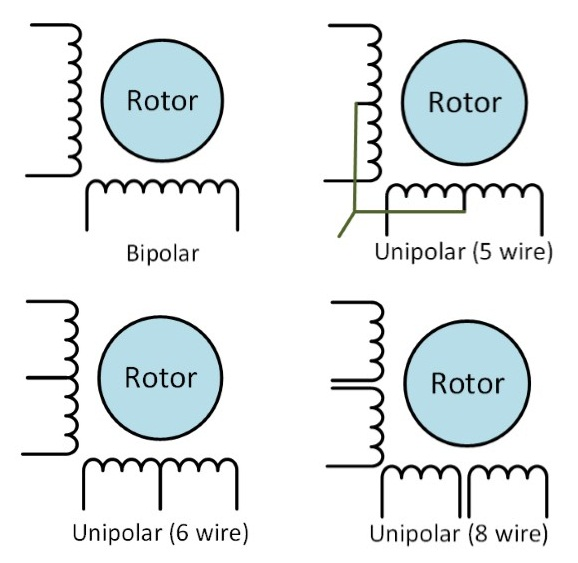
\includegraphics{/home/milav/Codes/MPMC/assets/imgs/181001_MCU_Question_Bank_Solved_html_3e590d621acc08fa.png}
\caption{}
\end{figure}

\textbf{Wiring Arrangements}

\begin{itemize}
\item
  \textbf{Unipolar (5-wire):} Only half of each coil is used at a time.
\item
  \textbf{Unipolar (6-wire):} Full coil use is possible for increased
  torque.
\item
  \textbf{Unipolar (8-wire):} Provides the greatest wiring flexibility
  (unipolar or bipolar operation).
\item
  \textbf{Bipolar (4-wire):} The coil current direction needs to be
  reversed for rotation direction control. This requires an H-bridge
  driver circuit.
\end{itemize}

\textbf{Stepper Motor Drive Modes}

\begin{enumerate}
\def\labelenumi{\arabic{enumi}.}
\item
  \textbf{Wave Drive (One-Phase On)}

  \begin{itemize}
  \item
    Simpliest to control.
  \item
    Only one coil is energized at a time.
  \item
    Lower torque and holding strength.
  \end{itemize}
\end{enumerate}

\begin{longtable}[]{@{}llll@{}}
\toprule
A & B & C & D \\
\midrule
\endhead
1 & 0 & 0 & 0 \\
0 & 1 & 0 & 0 \\
0 & 1 & 0 & 0 \\
0 & 0 & 0 & 1 \\
\bottomrule
\end{longtable}

\begin{enumerate}
\def\labelenumi{\arabic{enumi}.}
\item
  \textbf{Full-Step Drive (Two-Phase On)}

  \begin{itemize}
  \item
    Two coils are energized simultaneously.
  \item
    Provides increased torque compared to wave drive.
  \end{itemize}
\end{enumerate}

\begin{longtable}[]{@{}llll@{}}
\toprule
A & B & C & D \\
\midrule
\endhead
1 & 1 & 0 & 0 \\
0 & 1 & 1 & 0 \\
0 & 0 & 1 & 1 \\
1 & 0 & 0 & 1 \\
\bottomrule
\end{longtable}

\begin{figure}
\centering
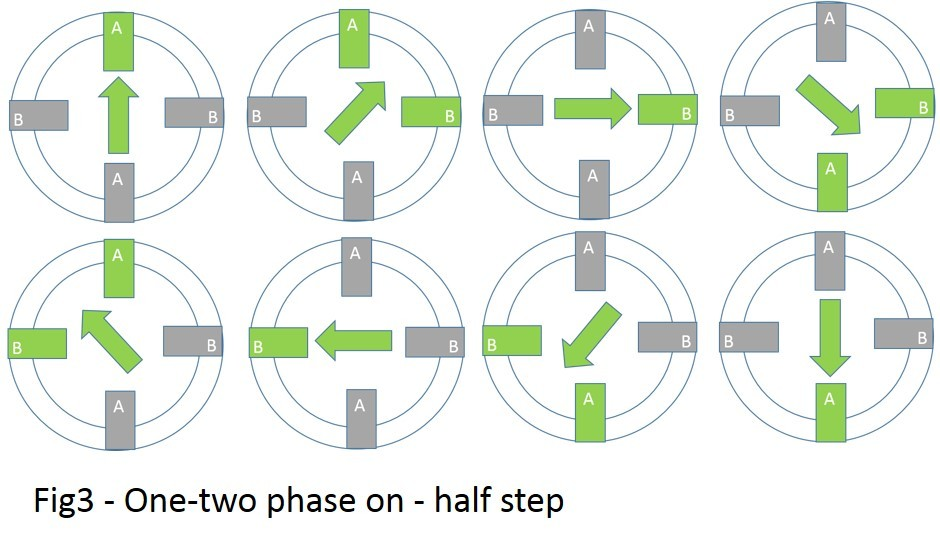
\includegraphics{/home/milav/Codes/MPMC/assets/imgs/181001_MCU_Question_Bank_Solved_html_ebfadda19e8e1674.png}
\caption{}
\end{figure}

\begin{enumerate}
\def\labelenumi{\arabic{enumi}.}
\item
  \textbf{Half-Step Drive}

  \begin{itemize}
  \item
    Alternates between wave drive and full-step drive.
  \item
    Doubles the effective resolution of the motor (smaller step angles).
  \item
    Maintains good torque levels.
  \end{itemize}
\end{enumerate}

\begin{longtable}[]{@{}llll@{}}
\toprule
A & B & C & D \\
\midrule
\endhead
1 & 0 & 0 & 0 \\
1 & 1 & 0 & 0 \\
0 & 1 & 0 & 0 \\
0 & 1 & 1 & 0 \\
0 & 0 & 1 & 0 \\
0 & 0 & 1 & 1 \\
0 & 0 & 0 & 1 \\
1 & 0 & 0 & 1 \\
\bottomrule
\end{longtable}

\begin{figure}
\centering
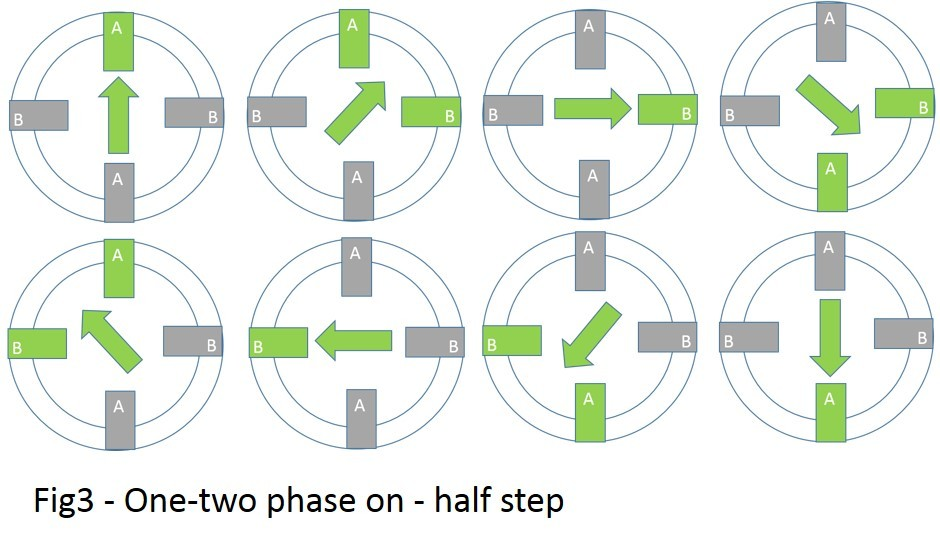
\includegraphics{/home/milav/Codes/MPMC/assets/imgs/181001_MCU_Question_Bank_Solved_html_ebfadda19e8e1674.png}
\caption{}
\end{figure}

\textbf{Interfacing with the 8051}

\begin{enumerate}
\def\labelenumi{\arabic{enumi}.}
\item
  \textbf{GPIO Pins:} Connect output pins from the 8051 to a compatible
  stepper motor driver.
\item
  \textbf{Stepper Motor Driver:}

  \begin{itemize}
  \item
    \textbf{ULN2003:} Simple and suitable for unipolar stepper motors.
  \item
    \textbf{H-bridge Drivers (e.g., L293D, A4988, etc.):} For bipolar
    motors, as they can reverse current flow.
  \end{itemize}
\item
  \textbf{Step Sequencing:} The 8051 generates the correct pulse
  sequence (wave, full, or half-step) to control the stepping pattern
  and direction of the motor.
\end{enumerate}

\hypertarget{5262-stepper-motor-interfacing-with-8051}{%
\paragraph{5.2.6.2. Stepper Motor Interfacing with
8051}\label{5262-stepper-motor-interfacing-with-8051}}

\textbf{Hardware Connections:}

\begin{figure}
\centering
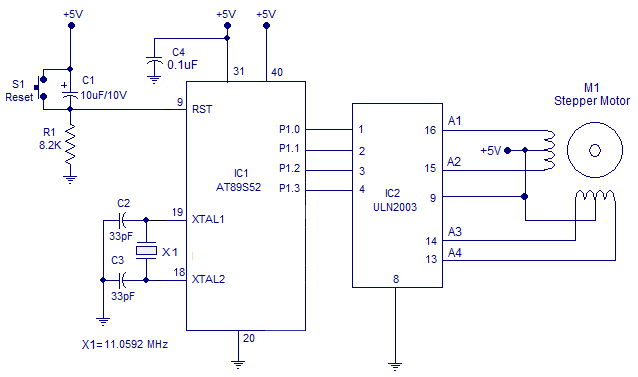
\includegraphics{/home/milav/Codes/MPMC/assets/imgs/181001_MCU_Question_Bank_Solved_html_2ba010187338c44e.png}
\caption{}
\end{figure}

Here's a breakdown of the connections:

\begin{itemize}
\item
  \textbf{Microcontroller (8051):}

  \begin{itemize}
  \item
    Port 1 (P1) is connected to the input pins of the ULN2003 (A1, A2,
    A3, and A4).
  \end{itemize}
\item
  \textbf{ULN2003 Driver:}

  \begin{itemize}
  \item
    Input pins (A1-A4) are connected to the microcontroller (P1.0-P1.3).
  \item
    Output pins (B1-B4) are connected to the stepper motor coils in the
    correct sequence according to the motor's wiring diagram.
  \end{itemize}
\item
  \textbf{Stepper Motor:}

  \begin{itemize}
  \item
    The four coils of the stepper motor are connected to the
    corresponding output pins (B1-B4) of the ULN2003 driver.
  \end{itemize}
\item
  \textbf{Power Supply:}

  \begin{itemize}
  \item
    The microcontroller and ULN2003 share a common 5V power supply.
  \end{itemize}
\end{itemize}

\textbf{ULN2003 (Function of ULN2003)}

The ULN2003 is a Darlington transistor array, which essentially acts as
an amplifier. It allows the low-current outputs of the microcontroller
to drive the higher current required by the stepper motor coils.

\textbf{Stepper Motor Driving Principle}

By applying specific pulse sequences to the stepper motor coils in a
particular order, the motor shaft rotates in steps. Different pulse
sequences can be used to achieve different rotation directions and
stepping patterns.

\textbf{Assembly Code Example}

\begin{Shaded}
\begin{Highlighting}[]
\NormalTok{; Define stepper motor step sequence (full step)}
\NormalTok{MOV R0, \#0001h  ; Initial step pattern (replace for different patterns)}

\NormalTok{; Loop to continuously drive the motor}
\NormalTok{MAIN\_LOOP:}
\NormalTok{    MOV P1, R0     ; Send step pattern to ULN2003}

\NormalTok{    ; Add delay for desired step speed (adjust delay value as needed)}
\NormalTok{    MOV R1, \#100  ; Set delay loop counter}
\NormalTok{    DELAY\_LOOP:}
\NormalTok{        DJNZ R1, DELAY\_LOOP}

\NormalTok{    ; Rotate step pattern for next step (modify for different patterns)}
\NormalTok{    RLC R0        ; Rotate left to shift bits for next step}
\NormalTok{    CJNE R0, \#0010h, MAIN\_LOOP  ; Check if completed a full rotation}
\NormalTok{    MOV R0, \#0001h              ; Reset step pattern if completed}

\NormalTok{JMP MAIN\_LOOP}
\end{Highlighting}
\end{Shaded}

\textbf{C Code Example}

\begin{Shaded}
\begin{Highlighting}[]
\PreprocessorTok{\#include }\ImportTok{\textless{}reg51.h\textgreater{}}

\DataTypeTok{void}\NormalTok{ delay}\OperatorTok{(}\DataTypeTok{unsigned} \DataTypeTok{int}\NormalTok{ ms}\OperatorTok{)} \OperatorTok{\{} \CommentTok{// Simple delay routine}
    \DataTypeTok{unsigned} \DataTypeTok{int}\NormalTok{ i}\OperatorTok{,}\NormalTok{ j}\OperatorTok{;}
    \ControlFlowTok{for} \OperatorTok{(}\NormalTok{i }\OperatorTok{=} \DecValTok{0}\OperatorTok{;}\NormalTok{ i }\OperatorTok{\textless{}}\NormalTok{ ms}\OperatorTok{;}\NormalTok{ i}\OperatorTok{++)} \OperatorTok{\{}
        \ControlFlowTok{for} \OperatorTok{(}\NormalTok{j }\OperatorTok{=} \DecValTok{0}\OperatorTok{;}\NormalTok{ j }\OperatorTok{\textless{}} \DecValTok{1275}\OperatorTok{;}\NormalTok{ j}\OperatorTok{++);}
    \OperatorTok{\}}
\OperatorTok{\}}

\DataTypeTok{unsigned} \DataTypeTok{char}\NormalTok{ step\_pattern}\OperatorTok{[]} \OperatorTok{=} \OperatorTok{\{}\BaseNTok{0x01}\OperatorTok{,} \BaseNTok{0x02}\OperatorTok{,} \BaseNTok{0x04}\OperatorTok{,} \BaseNTok{0x08}\OperatorTok{\};} \CommentTok{// Full step sequence (replace for different patterns)}
\DataTypeTok{int}\NormalTok{ step\_index }\OperatorTok{=} \DecValTok{0}\OperatorTok{;}

\DataTypeTok{void}\NormalTok{ main}\OperatorTok{()} \OperatorTok{\{}
    \ControlFlowTok{while} \OperatorTok{(}\DecValTok{1}\OperatorTok{)} \OperatorTok{\{}
\NormalTok{        P1 }\OperatorTok{=}\NormalTok{ step\_pattern}\OperatorTok{[}\NormalTok{step\_index}\OperatorTok{];} \CommentTok{// Send step pattern to ULN2003}

\NormalTok{        delay}\OperatorTok{(}\DecValTok{5}\OperatorTok{);} \CommentTok{// Adjust delay for desired step speed}

\NormalTok{        step\_index}\OperatorTok{++;} \CommentTok{// Move to the next step in the sequence}
        \ControlFlowTok{if} \OperatorTok{(}\NormalTok{step\_index }\OperatorTok{\textgreater{}=} \KeywordTok{sizeof}\OperatorTok{(}\NormalTok{step\_pattern}\OperatorTok{)} \OperatorTok{/} \KeywordTok{sizeof}\OperatorTok{(}\NormalTok{step\_pattern}\OperatorTok{[}\DecValTok{0}\OperatorTok{]))} \OperatorTok{\{}
\NormalTok{            step\_index }\OperatorTok{=} \DecValTok{0}\OperatorTok{;} \CommentTok{// Reset step index if completed a full rotation}
        \OperatorTok{\}}
    \OperatorTok{\}}
\OperatorTok{\}}
\end{Highlighting}
\end{Shaded}

\textbf{Explanation of the Code:}

\begin{itemize}
\item
  The code defines a step pattern which is a sequence of values
  representing the energized coils at each step.
\item
  A loop continuously outputs the step pattern to the ULN2003, causing
  the motor to rotate one step at a time.
\item
  The delay loop controls the speed of the motor's steps.
\item
  The assembly code uses bit manipulation (\texttt{RLC}) to rotate the
  step pattern for the next step.
\item
  The C code uses an array to store the step pattern and an index to
  keep track of the current step.
\end{itemize}

\hypertarget{53-adc-analog-to-digital-converter}{%
\subsection{5.3. ADC (Analog-to-Digital
Converter)}\label{53-adc-analog-to-digital-converter}}

\begin{itemize}
\item
  \textbf{Purpose:} ADCs are electronic circuits that convert continuous
  analog voltage signals into discrete digital representations. This is
  essential for microcontrollers, which primarily work with digital
  data.
\item
  \textbf{Process:}

  \begin{enumerate}
  \def\labelenumi{\arabic{enumi}.}
  \item
    \textbf{Sampling:} The ADC takes "snapshots" of the analog input
    signal at regular intervals.
  \item
    \textbf{Quantization:} Each sample's voltage level is compared to a
    reference voltage and mapped to a discrete digital value.
  \item
    \textbf{Output:} The result is a binary code representing the
    closest digital approximation of the analog input.
  \end{enumerate}
\item
  \textbf{Key Characteristics}

  \begin{itemize}
  \item
    \textbf{Resolution:} Number of bits in the output code (e.g., 8-bit,
    10-bit). Higher resolution means finer digital representations of
    the analog signal.
  \item
    \textbf{Sampling rate:} How frequently the ADC samples the analog
    input (measured in samples per second).
  \item
    \textbf{Accuracy:} How closely the digital output reflects the true
    analog input.
  \end{itemize}
\end{itemize}

\textbf{ADC0804 Overview}

\begin{itemize}
\item
  \textbf{Type:} Successive approximation ADC (SAR ADC).
\item
  \textbf{Features:}

  \begin{itemize}
  \item
    8-bit resolution (256 discrete output levels)
  \item
    Single analog input channel
  \item
    Requires an external clock signal to control conversion time
  \item
    TTL compatible for easy interfacing with microcontrollers
  \item
    Low power consumption
  \item
    Relatively simple and inexpensive
  \end{itemize}
\end{itemize}

\textbf{Pinout (20-pin DIP package)}

\begin{figure}
\centering
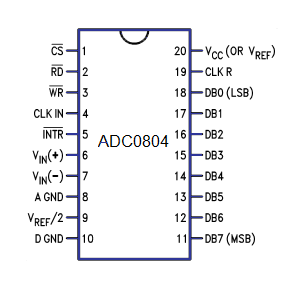
\includegraphics{/home/milav/Codes/MPMC/assets/imgs/181001_MCU_Question_Bank_Solved_html_3d8dc52f5e66fee0.png}
\caption{}
\end{figure}

\begin{itemize}
\item
  \textbf{Analog Input:}

  \begin{itemize}
  \item
    VIN(+) : Positive analog input
  \item
    VIN(-): Negative analog input (often connected to ground for
    single-ended operation)
  \end{itemize}
\item
  \textbf{Reference Voltage:}

  \begin{itemize}
  \item
    Vref/2: Reference voltage input (sets the range for conversion)
  \end{itemize}
\item
  \textbf{Control Signals:}

  \begin{itemize}
  \item
    CS: Chip Select (active low)
  \item
    RD: Read (active low)
  \item
    WR: Write (active low)
  \item
    INTR: Interrupt (active low, signals end of conversion)
  \item
    CLK IN: External clock input
  \end{itemize}
\item
  \textbf{Digital Outputs:}

  \begin{itemize}
  \item
    D0 - D7: 8-bit digital output
  \end{itemize}
\end{itemize}

\textbf{Typical Usage Scenario}

\begin{enumerate}
\def\labelenumi{\arabic{enumi}.}
\item
  \textbf{Connect Signals} Interface the ADC0804 with a microcontroller,
  providing necessary control signals and reading the digital output.
\item
  \textbf{Apply Reference Voltage:} Set the reference voltage (Vref/2)
  to determine the input voltage range you want to measure.
\item
  \textbf{Initiate Conversion:} Use the control signals (CS, RD, WR) to
  start an analog to digital conversion.
\item
  \textbf{Clocking:} Provide an external clock signal (if no internal
  clock is used) to drive the conversion process.
\item
  \textbf{Read Result:} When the conversion completes, signaled by the
  INTR pin or by polling, read the 8-bit digital output.
\end{enumerate}

\hypertarget{531-adc0804-interfacing}{%
\subsubsection{5.3.1. ADC0804
Interfacing}\label{531-adc0804-interfacing}}

\textbf{Assumptions}

\begin{itemize}
\item
  \textbf{ADC0804 Connections:}

  \begin{itemize}
  \item
    Analog Input (VIN+) to the signal you want to measure.
  \item
    VIN- to ground.
  \item
    Control Pins (CS, RD, WR, INTR) to 8051 I/O pins.
  \item
    Data Pins (D0-D7) to an 8051 port.
  \end{itemize}
\item
  \textbf{8051 Hardware:} We'll use Port 1 (P1) for the ADC data and
  sample control signals on the 8051.
\end{itemize}

\textbf{Hardware Setup}

\begin{figure}
\centering
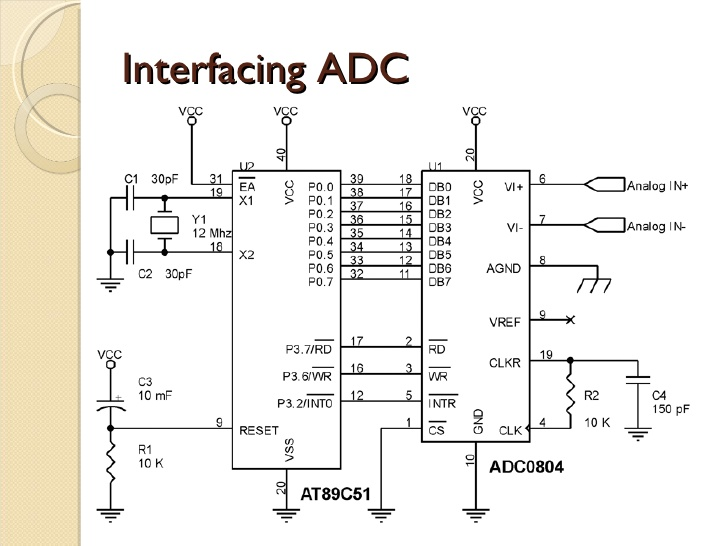
\includegraphics{/home/milav/Codes/MPMC/assets/imgs/181001_MCU_Question_Bank_Solved_html_b1e4e731f7178dfd.png}
\caption{}
\end{figure}

\begin{enumerate}
\def\labelenumi{\arabic{enumi}.}
\item
  \textbf{Connect ADC0804 and 8051:} Interface the ADC pins to your 8051
  microcontroller as described above.
\item
  \textbf{Reference Voltage:} Apply an appropriate reference voltage to
  the ADC's Vref/2 pin. This determines the full-scale input range.
\item
  \textbf{Clock Source:} If your ADC0804 doesn't have an internal clock,
  connect an external clock signal to the CLK IN pin.
\end{enumerate}

\textbf{Assembly Code}

\begin{Shaded}
\begin{Highlighting}[]
\NormalTok{;Assuming P1 is used for ADC0804, analog input to ADC channel 0}

\NormalTok{ORG 0000H ; Start code execution at address 0000H}

\NormalTok{ADC\_INIT:}
\NormalTok{    ; ... (Initialize any other necessary peripherals)}

\NormalTok{READ\_ADC:}
\NormalTok{    CLR P1.0  ; CS = 0 (Select ADC0804)}
\NormalTok{    CLR P1.1  ; WR = 0 (Start conversion)}
\NormalTok{    SETB P1.1 ; WR = 1}
\NormalTok{    ; Optionally, poll the INTR pin for conversion completion}

\NormalTok{    SETB P1.0 ; CS = 1}
\NormalTok{    CLR P1.2  ; RD = 0 (Read data)}
\NormalTok{    MOV A, P1 ; Read ADC value}
\NormalTok{    SETB P1.2 ; RD = 1}

\NormalTok{    ; ... (Utilize the ADC value stored in the Accumulator (A))}

\NormalTok{AJMP READ\_ADC ; Jump back to read ADC continuously}
\end{Highlighting}
\end{Shaded}

\textbf{C Code}

\begin{Shaded}
\begin{Highlighting}[]
\PreprocessorTok{\#include }\ImportTok{\textless{}reg51.h\textgreater{}}

\NormalTok{sbit CS   }\OperatorTok{=}\NormalTok{ P1}\OperatorTok{\^{}}\DecValTok{0}\OperatorTok{;}
\NormalTok{sbit WR   }\OperatorTok{=}\NormalTok{ P1}\OperatorTok{\^{}}\DecValTok{1}\OperatorTok{;}
\NormalTok{sbit RD   }\OperatorTok{=}\NormalTok{ P1}\OperatorTok{\^{}}\DecValTok{2}\OperatorTok{;}
\NormalTok{sbit INTR }\OperatorTok{=}\NormalTok{ P1}\OperatorTok{\^{}}\DecValTok{3}\OperatorTok{;} \CommentTok{// Check if your ADC setup uses the INTR pin}

\DataTypeTok{void}\NormalTok{ adc\_init}\OperatorTok{()} \OperatorTok{\{}
    \CommentTok{// ... (Initialize any other necessary peripherals)}
\OperatorTok{\}}

\DataTypeTok{unsigned} \DataTypeTok{char}\NormalTok{ read\_adc}\OperatorTok{()} \OperatorTok{\{}
    \DataTypeTok{unsigned} \DataTypeTok{char}\NormalTok{ adc\_value}\OperatorTok{;}

\NormalTok{    CS }\OperatorTok{=} \DecValTok{0}\OperatorTok{;}      \CommentTok{// Select the ADC0804}
\NormalTok{    WR }\OperatorTok{=} \DecValTok{0}\OperatorTok{;}      \CommentTok{// Start conversion}
\NormalTok{    WR }\OperatorTok{=} \DecValTok{1}\OperatorTok{;}
    \CommentTok{// Optionally, wait for INTR to go low for conversion completion}

\NormalTok{    CS }\OperatorTok{=} \DecValTok{1}\OperatorTok{;}
\NormalTok{    RD }\OperatorTok{=} \DecValTok{0}\OperatorTok{;}      \CommentTok{// Read data}
\NormalTok{    adc\_value }\OperatorTok{=}\NormalTok{ P1}\OperatorTok{;}
\NormalTok{    RD }\OperatorTok{=} \DecValTok{1}\OperatorTok{;}

    \ControlFlowTok{return}\NormalTok{ adc\_value}\OperatorTok{;}
\OperatorTok{\}}

\DataTypeTok{void}\NormalTok{ main}\OperatorTok{()} \OperatorTok{\{}
    \DataTypeTok{unsigned} \DataTypeTok{char}\NormalTok{ adc\_data}\OperatorTok{;}

\NormalTok{    adc\_init}\OperatorTok{();}

    \ControlFlowTok{while} \OperatorTok{(}\DecValTok{1}\OperatorTok{)} \OperatorTok{\{}
\NormalTok{        adc\_data }\OperatorTok{=}\NormalTok{ read\_adc}\OperatorTok{();}
        \CommentTok{// ... (Utilize the ADC value)}
    \OperatorTok{\}}
\OperatorTok{\}}
\end{Highlighting}
\end{Shaded}

\textbf{Important Notes}

\begin{itemize}
\item
  \textbf{Control Pins:} Adjust the pin assignments in the code if
  you're using different 8051 pins.
\item
  \textbf{Error Handling:} Implement error checks in production code.
\item
  \textbf{Timing:} Consider the ADC0804's conversion time and adjust
  delays or polling accordingly.
\item
  \textbf{Calculation:} Scale the raw ADC value to a meaningful voltage
  based on your reference voltage.
\end{itemize}

\hypertarget{54-dac-digital-to-analog-converter}{%
\subsection{5.4. DAC (Digital-to-Analog
Converter)}\label{54-dac-digital-to-analog-converter}}

\begin{itemize}
\item
  \textbf{Purpose:} DACs are electronic circuits that do the opposite of
  ADCs -- they convert digital codes into corresponding analog voltage
  levels. This allows microcontrollers to generate smooth analog signals
  for various applications.
\item
  \textbf{Process:}

  \begin{enumerate}
  \def\labelenumi{\arabic{enumi}.}
  \item
    \textbf{Digital Input:} The DAC accepts a binary code as input.
  \item
    \textbf{Reference Voltage:} A stable reference voltage determines
    the full-scale output range of the DAC.
  \item
    \textbf{Conversion:} The DAC generates an analog voltage
    proportional to the digital input code and the reference voltage.
  \end{enumerate}
\item
  \textbf{Key Characteristics:}

  \begin{itemize}
  \item
    \textbf{Resolution:} The number of bits in the input code (e.g.,
    8-bit, 10-bit). Higher resolution means more fine-grained analog
    output levels.
  \item
    \textbf{Accuracy:} How closely the analog output represents the
    target value based on the digital input.
  \item
    \textbf{Settling Time:} How quickly the DAC's output stabilizes to a
    new voltage after a change in the digital input.
  \end{itemize}
\end{itemize}

\textbf{DAC0808 Overview}

\begin{itemize}
\item
  \textbf{Type:} A common R-2R ladder type DAC.
\item
  \textbf{Features:}

  \begin{itemize}
  \item
    8-bit resolution (256 discrete output levels)
  \item
    Single analog output
  \item
    Reference current input to set output range
  \item
    Can be used in multiplying mode for greater precision
  \item
    TTL compatible for easy interfacing with microcontrollers
  \item
    Fast settling time
  \end{itemize}
\end{itemize}

\textbf{Pinout (16-pin DIP package)}

\begin{itemize}
\item
  \textbf{Digital Inputs:}

  \begin{itemize}
  \item
    I0 - I7: Least significant bit (LSB) to most significant bit (MSB)
  \end{itemize}
\item
  \textbf{Reference Current}

  \begin{itemize}
  \item
    Iref: Determines the output current (and thus the output voltage
    range)
  \end{itemize}
\item
  \textbf{Analog Output}

  \begin{itemize}
  \item
    IOUT: The analog output current
  \end{itemize}
\item
  \textbf{Other}

  \begin{itemize}
  \item
    Vcc: +5V Power supply
  \item
    GND: Ground
  \end{itemize}
\end{itemize}

\textbf{Typical Usage Scenario}

\begin{enumerate}
\def\labelenumi{\arabic{enumi}.}
\item
  \textbf{Connect Signals:} Interface the DAC0808 with a microcontroller
  to send digital data.
\item
  \textbf{Set Reference Current:} Apply the required reference current
  to Iref. This will determine the maximum output voltage and the step
  size per digital input change.
\item
  \textbf{Send Digital Code:} Write the 8-bit digital code to the DAC's
  input pins.
\item
  \textbf{Output:} The DAC outputs a corresponding analog current at
  IOUT. Often, this current is converted to an analog voltage by using
  an external op-amp circuit.
\end{enumerate}

\hypertarget{541-dac0808-interfacing}{%
\subsubsection{5.4.1. DAC0808
Interfacing}\label{541-dac0808-interfacing}}

\textbf{Assumptions}

\begin{itemize}
\item
  \textbf{DAC0808 Connections:}

  \begin{itemize}
  \item
    Digital inputs (I0-I7) connected to an 8051 port.
  \item
    Iref connected to a suitable current source to set the output range.
  \item
    External op-amp circuit (if needed) to convert the DAC output
    current (IOUT) into a usable voltage.
  \end{itemize}
\item
  \textbf{8051 Hardware:} We'll use Port 1 (P1) for sending data to the
  DAC0808.
\end{itemize}

\textbf{Hardware Setup}

\begin{figure}
\centering
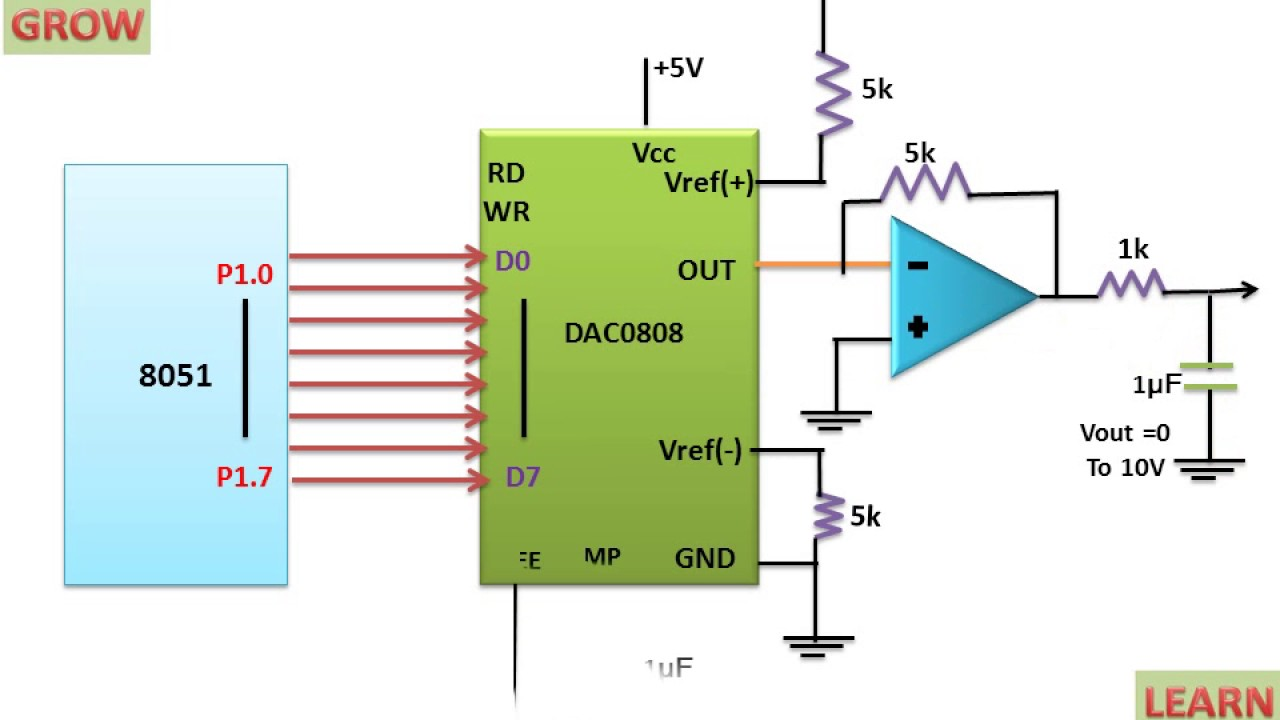
\includegraphics{/home/milav/Codes/MPMC/assets/imgs/181001_MCU_Question_Bank_Solved_html_145f316714bc984f.png}
\caption{}
\end{figure}

\begin{enumerate}
\def\labelenumi{\arabic{enumi}.}
\item
  \textbf{Connect DAC0808 and 8051:} Interface the pins to your 8051 as
  described above.
\item
  \textbf{Reference Current:} Apply a suitable current to Iref. This
  determines the output voltage range for your application.
\item
  \textbf{Op-amp Circuit (Optional):} If you want a voltage output from
  the DAC, design an op-amp circuit to convert the IOUT current into a
  voltage.
\end{enumerate}

\textbf{Assembly Code}

\begin{Shaded}
\begin{Highlighting}[]
\NormalTok{;Assuming P1 is used for the DAC0808 data}

\NormalTok{ORG 0000H ; Initialize program start at address 0000H}

\NormalTok{SET\_DAC\_VALUE:}
\NormalTok{    MOV A, \#\textless{}your\_digital\_value\textgreater{}  ; Load desired digital value (0{-}255)}
\NormalTok{    MOV P1, A                     ; Send data to DAC0808}

\NormalTok{    ; ... (Add delays if necessary based on DAC settling time)}

\NormalTok{    AJMP SET\_DAC\_VALUE            ; Jump back to update DAC value}
\end{Highlighting}
\end{Shaded}

\textbf{C Code}

\begin{Shaded}
\begin{Highlighting}[]
\PreprocessorTok{\#include }\ImportTok{\textless{}reg51.h\textgreater{}}

\DataTypeTok{void}\NormalTok{ set\_dac\_value}\OperatorTok{(}\DataTypeTok{unsigned} \DataTypeTok{char}\NormalTok{ value}\OperatorTok{)} \OperatorTok{\{}
\NormalTok{    P1 }\OperatorTok{=}\NormalTok{ value}\OperatorTok{;}  \CommentTok{// Send data to DAC0808}
    \CommentTok{// ... (Add delays if necessary based on DAC settling time)}
\OperatorTok{\}}

\DataTypeTok{void}\NormalTok{ main}\OperatorTok{()} \OperatorTok{\{}
    \DataTypeTok{unsigned} \DataTypeTok{char}\NormalTok{ dac\_value }\OperatorTok{=} \DecValTok{0}\OperatorTok{;}

    \ControlFlowTok{while} \OperatorTok{(}\DecValTok{1}\OperatorTok{)} \OperatorTok{\{}
\NormalTok{        set\_dac\_value}\OperatorTok{(}\NormalTok{dac\_value}\OperatorTok{);}
        \CommentTok{// ... (Code to change dac\_value over time to create output patterns)}
    \OperatorTok{\}}
\OperatorTok{\}}
\end{Highlighting}
\end{Shaded}

\textbf{Important Notes}

\begin{itemize}
\item
  \textbf{Digital Value:} In the code, replace
  \texttt{\textless{}your\_digital\_value\textgreater{}} with the
  desired output (0-255, representing 0 to your maximum output voltage).
\item
  \textbf{Iref:} Carefully choose the current at Iref to give you the
  desired full-scale output voltage range.
\item
  \textbf{Settling Time:} Your DAC0808 datasheet will specify the
  settling time. Consider adding delays if needed to ensure the analog
  output has stabilized before taking critical measurements.
\item
  \textbf{Op-amp:} If you require a voltage output, design a suitable
  op-amp circuit around the IOUT pin.
\end{itemize}

\hypertarget{542-generate-ramp-signal-using-dac}{%
\subsubsection{5.4.2. Generate Ramp Signal using
DAC}\label{542-generate-ramp-signal-using-dac}}

\textbf{Ramp Signal Basics}

\begin{itemize}
\item
  A ramp signal linearly increases or decreases in voltage over time.
\item
  We'll create an ascending ramp (increasing in value).
\end{itemize}

\textbf{Assembly Code}

\begin{Shaded}
\begin{Highlighting}[]
\NormalTok{ORG 0000H}

\NormalTok{MAIN\_LOOP:}
\NormalTok{    MOV R0, \#00H  ; Initialize counter variable}

\NormalTok{RAMP\_UP:}
\NormalTok{    MOV A, R0     ; Load value into the accumulator}
\NormalTok{    MOV P1, A     ; Send the value to DAC}
\NormalTok{    INC R0        ; Increment counter}
\NormalTok{    CJNE R0, \#FFh, RAMP\_UP  ; Repeat until max value (255)}

\NormalTok{    ; Option 1: Reset and repeat}
\NormalTok{    MOV R0, \#00H}
\NormalTok{    JMP RAMP\_UP}

\NormalTok{    ; Option 2: Ramp down (uncomment if needed)}
\NormalTok{    ;RAMP\_DOWN:}
\NormalTok{    ;    DJNZ R0, RAMP\_DOWN  ; Decrement and repeat until 0}
\NormalTok{    ;    JMP RAMP\_UP         ; Loop back to ramp up}

\NormalTok{    JMP MAIN\_LOOP  ; Loop back for continuous ramp generation}
\end{Highlighting}
\end{Shaded}

\textbf{C Code}

\begin{Shaded}
\begin{Highlighting}[]
\PreprocessorTok{\#include }\ImportTok{\textless{}reg51.h\textgreater{}}

\DataTypeTok{void}\NormalTok{ delay}\OperatorTok{(}\DataTypeTok{unsigned} \DataTypeTok{int}\NormalTok{ ms}\OperatorTok{)} \OperatorTok{\{} \CommentTok{// Simple delay routine}
    \DataTypeTok{unsigned} \DataTypeTok{int}\NormalTok{ i}\OperatorTok{,}\NormalTok{ j}\OperatorTok{;}
    \ControlFlowTok{for} \OperatorTok{(}\NormalTok{i }\OperatorTok{=} \DecValTok{0}\OperatorTok{;}\NormalTok{ i }\OperatorTok{\textless{}}\NormalTok{ ms}\OperatorTok{;}\NormalTok{ i}\OperatorTok{++)} \OperatorTok{\{}
        \ControlFlowTok{for} \OperatorTok{(}\NormalTok{j }\OperatorTok{=} \DecValTok{0}\OperatorTok{;}\NormalTok{ j }\OperatorTok{\textless{}} \DecValTok{1275}\OperatorTok{;}\NormalTok{ j}\OperatorTok{++);}
    \OperatorTok{\}}
\OperatorTok{\}}

\DataTypeTok{void}\NormalTok{ main}\OperatorTok{()} \OperatorTok{\{}
    \DataTypeTok{unsigned} \DataTypeTok{char}\NormalTok{ value }\OperatorTok{=} \DecValTok{0}\OperatorTok{;}

    \ControlFlowTok{while} \OperatorTok{(}\DecValTok{1}\OperatorTok{)} \OperatorTok{\{}
        \ControlFlowTok{for} \OperatorTok{(}\NormalTok{value }\OperatorTok{=} \DecValTok{0}\OperatorTok{;}\NormalTok{ value }\OperatorTok{\textless{}} \DecValTok{255}\OperatorTok{;}\NormalTok{ value}\OperatorTok{++)} \OperatorTok{\{}
\NormalTok{            P1 }\OperatorTok{=}\NormalTok{ value}\OperatorTok{;}   \CommentTok{// Send value to DAC}
\NormalTok{            delay}\OperatorTok{(}\DecValTok{5}\OperatorTok{);}     \CommentTok{// Adjust delay for ramp speed}
        \OperatorTok{\}}

        \CommentTok{// Option 1: Reset and repeat}
        \CommentTok{// value = 0;}

        \CommentTok{// Option 2: Ramp down (uncomment if needed)}
        \CommentTok{// for (value = 255; value \textgreater{} 0; value{-}{-}) \{}
        \CommentTok{//    P1 = value;}
        \CommentTok{//    delay(5);}
        \CommentTok{//\}}
    \OperatorTok{\}}
\OperatorTok{\}}
\end{Highlighting}
\end{Shaded}

\textbf{Explanation}

\begin{itemize}
\item
  \textbf{Counter:} We use a variable (R0 in assembly, \texttt{value} in
  C) to track the output value.
\item
  \textbf{Loop:} The code continuously increments the output value,
  sending it to the DAC.
\item
  \textbf{Delay:} Adjust the delay for controlling the ramp's speed.
\item
  \textbf{Options:} I've included options to reset the ramp or to create
  a "sawtooth" pattern by both ramping up and down.
\end{itemize}

\textbf{Important:}

\begin{itemize}
\item
  \textbf{DAC Settling Time:} If your DAC has a significant settling
  time, you might need more precise delays instead of the simple
  software delay shown here.
\end{itemize}

\hypertarget{543-generate-triangular-wave-using-dac}{%
\subsubsection{5.4.3. Generate Triangular wave using
DAC}\label{543-generate-triangular-wave-using-dac}}

\textbf{Understanding Triangular Waves}

\begin{itemize}
\item
  A triangular wave linearly rises to a peak and then linearly falls to
  a minimum value, forming a triangle-like shape.
\end{itemize}

\textbf{Code Example (Assembly)}

\begin{Shaded}
\begin{Highlighting}[]
\NormalTok{ORG 0000H}

\NormalTok{MAIN\_LOOP:}
\NormalTok{    MOV R0, \#00H  ; Initialize counter variable}
\NormalTok{    MOV R1, \#01H  ; Flag to track direction (1: up, 0: down)}

\NormalTok{TRIANGLE\_GEN:}
\NormalTok{    MOV A, R0     ; Load value into the accumulator}
\NormalTok{    MOV P1, A     ; Send the value to DAC}

\NormalTok{    JNB R1, ASCENDING ; Check flag}
\NormalTok{    DJNZ R0, TRIANGLE\_GEN  ; Decrement if in descending phase}
\NormalTok{    JMP NEXT}

\NormalTok{ASCENDING:}
\NormalTok{    INC R0        ; Increment if in ascending phase}
\NormalTok{    CJNE R0, \#FFh, TRIANGLE\_GEN  ; Check if reached max value}

\NormalTok{NEXT:}
\NormalTok{    CPL R1        ; Toggle the direction flag}
\NormalTok{    JMP TRIANGLE\_GEN}
\end{Highlighting}
\end{Shaded}

\textbf{Code Example (C)}

\begin{Shaded}
\begin{Highlighting}[]
\PreprocessorTok{\#include }\ImportTok{\textless{}reg51.h\textgreater{}}

\DataTypeTok{void}\NormalTok{ delay}\OperatorTok{(}\DataTypeTok{unsigned} \DataTypeTok{int}\NormalTok{ ms}\OperatorTok{)} \OperatorTok{\{} \CommentTok{// Simple delay routine}
    \DataTypeTok{unsigned} \DataTypeTok{int}\NormalTok{ i}\OperatorTok{,}\NormalTok{ j}\OperatorTok{;}
    \ControlFlowTok{for} \OperatorTok{(}\NormalTok{i }\OperatorTok{=} \DecValTok{0}\OperatorTok{;}\NormalTok{ i }\OperatorTok{\textless{}}\NormalTok{ ms}\OperatorTok{;}\NormalTok{ i}\OperatorTok{++)} \OperatorTok{\{}
        \ControlFlowTok{for} \OperatorTok{(}\NormalTok{j }\OperatorTok{=} \DecValTok{0}\OperatorTok{;}\NormalTok{ j }\OperatorTok{\textless{}} \DecValTok{1275}\OperatorTok{;}\NormalTok{ j}\OperatorTok{++);}
    \OperatorTok{\}}
\OperatorTok{\}}

\DataTypeTok{void}\NormalTok{ main}\OperatorTok{()} \OperatorTok{\{}
    \DataTypeTok{unsigned} \DataTypeTok{char}\NormalTok{ value }\OperatorTok{=} \DecValTok{0}\OperatorTok{;}
    \DataTypeTok{int}\NormalTok{ direction }\OperatorTok{=} \DecValTok{1}\OperatorTok{;}  \CommentTok{// 1: ascending, 0: descending}

    \ControlFlowTok{while} \OperatorTok{(}\DecValTok{1}\OperatorTok{)} \OperatorTok{\{}
\NormalTok{       P1 }\OperatorTok{=}\NormalTok{ value}\OperatorTok{;}
\NormalTok{       delay}\OperatorTok{(}\DecValTok{5}\OperatorTok{);}

       \ControlFlowTok{if} \OperatorTok{(}\NormalTok{direction}\OperatorTok{)} \OperatorTok{\{}
\NormalTok{           value}\OperatorTok{++;}
           \ControlFlowTok{if} \OperatorTok{(}\NormalTok{value }\OperatorTok{==} \DecValTok{255}\OperatorTok{)} \OperatorTok{\{}
\NormalTok{               direction }\OperatorTok{=} \DecValTok{0}\OperatorTok{;} \CommentTok{// Start descending}
           \OperatorTok{\}}
       \OperatorTok{\}} \ControlFlowTok{else} \OperatorTok{\{}
\NormalTok{           value}\OperatorTok{{-}{-};}
           \ControlFlowTok{if} \OperatorTok{(}\NormalTok{value }\OperatorTok{==} \DecValTok{0}\OperatorTok{)} \OperatorTok{\{}
\NormalTok{               direction }\OperatorTok{=} \DecValTok{1}\OperatorTok{;} \CommentTok{// Start ascending}
           \OperatorTok{\}}
       \OperatorTok{\}}
    \OperatorTok{\}}
\OperatorTok{\}}
\end{Highlighting}
\end{Shaded}

\textbf{Explanation}

\begin{itemize}
\item
  \textbf{Counter:} Tracks the current output value (\texttt{R0} in
  assembly, \texttt{value} in C).
\item
  \textbf{Direction Flag:} Indicates whether the wave is ascending or
  descending.
\item
  \textbf{Logic:} The code increments the output until it reaches a
  maximum, then decrements until it reaches a minimum, continuously
  toggling the direction.
\end{itemize}

\textbf{Important Notes}

\begin{itemize}
\item
  \textbf{DAC Setup:} Ensure your DAC0808 is connected and configured
  correctly.
\item
  \textbf{Delay:} Adjust the delay to change the frequency of the
  triangular wave.
\item
  \textbf{Oscilloscope:} It's best to visualize the output on an
  oscilloscope to verify the waveform shape.
\end{itemize}

\hypertarget{55-real-world-applications}{%
\subsection{5.5. Real-World
Applications}\label{55-real-world-applications}}

Microcontrollers are incredibly versatile and find an astounding range
of uses across industries.

Here's a breakdown of applications in various fields:

\textbf{1. Consumer Electronics}

\begin{itemize}
\item
  \textbf{Televisions and Remote Controls:} Controlling picture
  settings, channel selection, volume, and smart features.
\item
  \textbf{Home Appliances:} Managing functions in washing machines,
  refrigerators, microwave ovens, air conditioners, etc.
\item
  \textbf{Personal Computers:} Peripherals (keyboard, mouse, printer),
  disk drives, power supplies.
\item
  \textbf{Toys and Gadgets:} Drones, remote control cars, electronic
  games, smart gadgets.
\end{itemize}

\textbf{2. Automotive Industry}

\begin{itemize}
\item
  \textbf{Engine Control Modules (ECM):} Optimizing fuel injection,
  ignition timing, emissions control, and overall engine performance.
\item
  \textbf{Anti-lock Braking Systems (ABS):} Preventing wheel lockup
  during hard braking.
\item
  \textbf{Airbag Systems:} Deployment timing and force control.
\item
  \textbf{Climate Control:} Maintaining desired temperature and
  regulating airflow.
\item
  \textbf{Infotainment Systems:} Navigation, audio/video players,
  Bluetooth connectivity
\item
  \textbf{Dashboard Displays:} Speedometers, tachometers, fuel level,
  warning lights.
\end{itemize}

\textbf{3. Medical Devices}

\begin{itemize}
\item
  \textbf{Patient Monitoring Systems:} Heart rate monitors, blood
  pressure monitors, glucose monitors.
\item
  \textbf{Therapeutic Devices:} Insulin pumps, pacemakers, hearing aids.
\item
  \textbf{Diagnostic Equipment:} X-ray machines, MRI scanners, lab
  analysis.
\end{itemize}

\textbf{4. Industrial Automation}

\begin{itemize}
\item
  \textbf{Robotics:} Precision control of robotic arms and assembly line
  robots
\item
  \textbf{Process Control:} Regulating temperature, pressure, flow rates
  in manufacturing processes.
\item
  \textbf{Motor Control:} Driving conveyor belts, pumps, and other
  industrial machinery
\item
  \textbf{Programmable Logic Controllers (PLCs):} Automating complex
  industrial processes.
\end{itemize}

\textbf{5. Building Automation}

\begin{itemize}
\item
  \textbf{Lighting Control:} Smart lighting systems for energy
  efficiency and ambiance control.
\item
  \textbf{HVAC Systems:} Temperature regulation, ventilation, and air
  quality control.
\item
  \textbf{Security Systems:} Access control, intruder alarms,
  surveillance systems.
\end{itemize}

\textbf{6. Other Notable Fields}

\begin{itemize}
\item
  \textbf{Aerospace and Defense:} Flight control systems, missile
  guidance, radar systems
\item
  \textbf{Telecommunications:} Cellular base stations, network switches,
  routers.
\item
  \textbf{Agriculture:} Precision irrigation systems, automated crop
  monitoring, livestock tracking.
\item
  \textbf{Energy Management:} Smart power grids, solar inverters,
  battery management systems.
\end{itemize}

\textbf{Key Reasons for Microcontroller Dominance}

\begin{itemize}
\item
  \textbf{Compact Size:} Integration of processor, memory, and I/O on a
  single chip.
\item
  \textbf{Low Cost:} Mass production makes them highly affordable.
\item
  \textbf{Flexibility:} Programmable to perform a wide range of tasks.
\item
  \textbf{Reliability:} Robust components with long lifespans.
\item
  \textbf{Low Power Consumption:} Ideal for battery-powered
  applications.
\end{itemize}

\hypertarget{551-temperature-control-system-using-an-lm35-sensor}{%
\subsubsection{5.5.1. Temperature control system using an LM35
sensor}\label{551-temperature-control-system-using-an-lm35-sensor}}

\textbf{Core Components}

\begin{enumerate}
\def\labelenumi{\arabic{enumi}.}
\item
  \textbf{Temperature Sensor (LM35):}

  \begin{itemize}
  \item
    Converts ambient temperature into an analog voltage signal.
  \item
    Output voltage is directly proportional to temperature in degrees
    Celsius.
  \end{itemize}
\item
  \textbf{Analog-to-Digital Converter (ADC0804/0808):}

  \begin{itemize}
  \item
    Converts the analog voltage from the LM35 to a digital value.
  \item
    Communicates with the 8051 using digital control signals.
  \end{itemize}
\item
  \textbf{8051 Microcontroller:}

  \begin{itemize}
  \item
    Reads the digital temperature value from the ADC.
  \item
    Compares the temperature to a setpoint (desired temperature).
  \item
    Generates control signals to drive the output device.
  \end{itemize}
\item
  \textbf{Output Device (e.g., Relay Module, Fan, Heater):}

  \begin{itemize}
  \item
    Controlled by the 8051 to regulate temperature.
  \item
    Turns on/off or adjusts its output to maintain the desired
    temperature.
  \end{itemize}
\end{enumerate}

\textbf{Block Diagram}

\begin{figure}
\centering
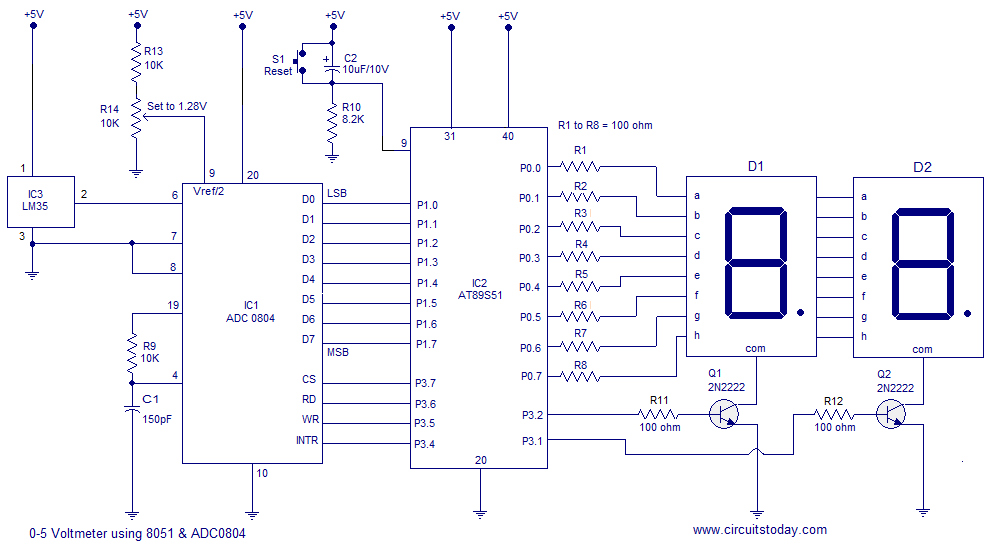
\includegraphics{/home/milav/Codes/MPMC/assets/imgs/181001_MCU_Question_Bank_Solved_html_75b4db4005f407f7.png}
\caption{}
\end{figure}

\begin{itemize}
\item
  \textbf{LM35 Temperature Sensor} -\textgreater{} \textbf{ADC0804/0808}
  -\textgreater{} \textbf{8051 Microcontroller} -\textgreater{}
  \textbf{Output Device (Relay, Fan, Heater)}
\end{itemize}

\textbf{Data Flow}

\begin{enumerate}
\def\labelenumi{\arabic{enumi}.}
\item
  The LM35 sensor produces an analog voltage corresponding to the
  current temperature.
\item
  The ADC0804/0808 converts this analog voltage into a digital value.
\item
  The 8051 microcontroller reads this digital value.
\item
  The 8051 compares the actual temperature with the setpoint (desired
  temperature).
\item
  The 8051 generates appropriate control signals based on the comparison
  result.
\item
  These control signals drive the output device to increase or decrease
  the temperature accordingly.
\end{enumerate}

\textbf{Additional Considerations}

\begin{itemize}
\item
  \textbf{Hysteresis:} Implement a small hysteresis band to prevent
  rapid on/off switching around the setpoint, reducing output device
  wear and tear.
\item
  \textbf{Display:} Incorporate an LCD or LED display to visualize the
  current temperature.
\item
  \textbf{User Input:} Add buttons or a potentiometer to adjust the
  desired setpoint.
\end{itemize}

\textbf{Example Scenario}

Let's say you want to maintain a room's temperature around 25 °C:

\begin{enumerate}
\def\labelenumi{\arabic{enumi}.}
\item
  The 8051 continuously reads the temperature value from the ADC.
\item
  If the temperature falls below 24 °C, the 8051 activates a heater.
\item
  If the temperature rises above 26 °C, the 8051 activates a fan.
\end{enumerate}

\hypertarget{552-gsm-based-security-system}{%
\subsubsection{5.5.2. GSM based Security
System}\label{552-gsm-based-security-system}}

\textbf{Components:}

\begin{enumerate}
\def\labelenumi{\arabic{enumi}.}
\item
  \textbf{Microcontroller (8051):}

  \begin{itemize}
  \item
    The central processing unit (CPU) of the system.
  \item
    Reads sensor data, controls the system's logic, and communicates
    with other components.
  \end{itemize}
\item
  \textbf{GSM Modem:}

  \begin{itemize}
  \item
    Enables communication with the GSM network (mobile cellular
    network).
  \item
    Used for sending SMS alerts or making emergency calls.
  \end{itemize}
\item
  \textbf{Sensors:}

  \begin{itemize}
  \item
    Detect security breaches or environmental changes (e.g., door/window
    contacts, PIR sensors, smoke detectors, gas sensors).
  \item
    Provide input signals to the microcontroller.
  \end{itemize}
\item
  \textbf{Relay Driver:}

  \begin{itemize}
  \item
    Drives relays that control external devices like alarms, lights, or
    door locks.
  \item
    The microcontroller sends control signals to the relay driver, which
    activates the relays accordingly.
  \end{itemize}
\item
  \textbf{Switches:}

  \begin{itemize}
  \item
    Allow manual user interaction with the system (e.g.,
    arming/disarming the alarm, controlling lights).
  \item
    Provide input signals to the microcontroller.
  \end{itemize}
\item
  \textbf{Power Supply:}

  \begin{itemize}
  \item
    Provides power to all the components of the system.
  \end{itemize}
\end{enumerate}

\begin{figure}
\centering
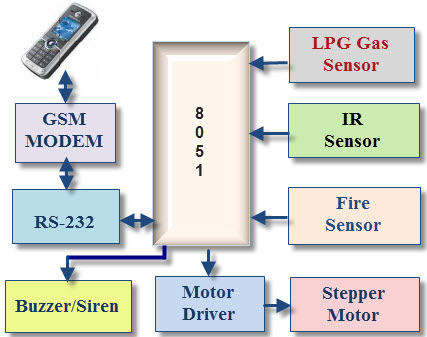
\includegraphics{/home/milav/Codes/MPMC/assets/imgs/181001_MCU_Question_Bank_Solved_html_eec44dfa48ebc913.png}
\caption{}
\end{figure}

\textbf{Data Flow:}

\begin{enumerate}
\def\labelenumi{\arabic{enumi}.}
\item
  \textbf{Sensors:} Continuously monitor the environment for security
  threats.
\item
  \textbf{Microcontroller:}

  \begin{itemize}
  \item
    Reads sensor data and processes it to detect security breaches.
  \item
    If a breach is detected, the microcontroller triggers an alarm and
    sends SMS alerts or makes emergency calls.
  \end{itemize}
\item
  \textbf{GSM Modem:}

  \begin{itemize}
  \item
    Communicates with the mobile network based on the microcontroller's
    instructions.
  \item
    Sends SMS alerts or initiates emergency calls to predefined numbers.
  \end{itemize}
\item
  \textbf{Relay Driver:}

  \begin{itemize}
  \item
    Receives control signals from the microcontroller.
  \item
    Activates or deactivates relays to control external devices like
    alarms, lights, or door locks.
  \end{itemize}
\item
  \textbf{Switches:}

  \begin{itemize}
  \item
    Provide user input to the microcontroller for actions like
    arming/disarming the system or controlling lights manually.
  \end{itemize}
\end{enumerate}

\hypertarget{553-rpm-meter}{%
\subsubsection{5.5.3. RPM meter}\label{553-rpm-meter}}

\textbf{Core Components}

\begin{enumerate}
\def\labelenumi{\arabic{enumi}.}
\item
  \textbf{Rotation Sensor:}

  \begin{itemize}
  \item
    Generates pulses proportional to the rotational speed of the shaft
    you wish to measure. Several types are common:

    \begin{itemize}
    \item
      \textbf{Inductive Pickup:} Detects passing gear teeth or keyways
      (good for robust applications).
    \item
      \textbf{Hall Effect Sensor:} Detects changes in the magnetic field
      created by magnets attached to the rotating shaft.
    \item
      \textbf{Optical Sensor:} Detects light/dark patterns on a disc
      attached to the shaft.
    \end{itemize}
  \end{itemize}
\item
  \textbf{Signal Conditioning Circuit:}

  \begin{itemize}
  \item
    \textbf{Amplification:} Boosts the sensor signal to a level the
    microcontroller can work with (often 0-5V).
  \item
    \textbf{Noise Filtering:} Removes unwanted noise that could corrupt
    the pulse detection.
  \end{itemize}
\item
  \textbf{8051 Microcontroller:}

  \begin{itemize}
  \item
    \textbf{Pulse Counting:} Counts the number of pulses from the sensor
    in a fixed time interval.
  \item
    \textbf{RPM Calculation:} Converts the pulse count over a known time
    interval into the revolutions per minute (RPM) value.
  \item
    \textbf{Optional Output:} Can drive a display or transmit RPM data
    over a communication bus.
  \end{itemize}
\item
  \textbf{Display (Optional)}

  \begin{itemize}
  \item
    Presents the calculated RPM to the user. Common options:

    \begin{itemize}
    \item
      \textbf{LCD:} Alphanumeric display for showing numerical RPM
      values.
    \item
      \textbf{LED Bar Graph:} A visual representation of increasing
      speed.
    \end{itemize}
  \end{itemize}
\end{enumerate}

\textbf{Block Diagram}

\begin{figure}
\centering
\includegraphics{/home/milav/Codes/MPMC/assets/imgs/181001_MCU_Question_Bank_Solved_html_b8fc2fb4587e8a0f.png}
\caption{}
\end{figure}

\textbf{Data Flow}

\begin{enumerate}
\def\labelenumi{\arabic{enumi}.}
\item
  \textbf{Sensor:} Generates electrical pulses corresponding to each
  rotation of the shaft.
\item
  \textbf{Signal Conditioning:} Cleans and amplifies the sensor signal
  for the microcontroller.
\item
  \textbf{8051:}

  \begin{itemize}
  \item
    Measures the time between pulses or counts pulses in a fixed time
    interval.
  \item
    Calculates the RPM based on the pulse measurement.
  \end{itemize}
\item
  \textbf{Output:} Sends the calculated RPM to a display or other
  communication channels.
\end{enumerate}

\textbf{Example Calculation}

If the sensor setup generates 1 pulse per rotation, and the 8051 counts
60 pulses in one second:

\begin{itemize}
\item
  RPM = 60 pulses per second * 60 seconds per minute = 3600 RPM
\end{itemize}

\textbf{Enhancements}

\begin{itemize}
\item
  \textbf{Multiple Sensors:} Use additional sensors for more accurate
  pulse counting to increase precision.
\item
  \textbf{Averaging:} Calculate RPM over several periods and average
  them for a smoother reading.
\item
  \textbf{User Interface:} Add buttons or a potentiometer to select
  different display modes or trigger calibration routines.
\end{itemize}

\end{document}
